\documentclass[twoside]{book}

% Packages required by doxygen
\usepackage{fixltx2e}
\usepackage{calc}
\usepackage{doxygen}
\usepackage[export]{adjustbox} % also loads graphicx
\usepackage{graphicx}
\usepackage[utf8]{inputenc}
\usepackage{makeidx}
\usepackage{multicol}
\usepackage{multirow}
\PassOptionsToPackage{warn}{textcomp}
\usepackage{textcomp}
\usepackage[nointegrals]{wasysym}
\usepackage[table]{xcolor}

% Font selection
\usepackage[T1]{fontenc}
\usepackage[scaled=.90]{helvet}
\usepackage{courier}
\usepackage{amssymb}
\usepackage{sectsty}
\renewcommand{\familydefault}{\sfdefault}
\allsectionsfont{%
  \fontseries{bc}\selectfont%
  \color{darkgray}%
}
\renewcommand{\DoxyLabelFont}{%
  \fontseries{bc}\selectfont%
  \color{darkgray}%
}
\newcommand{\+}{\discretionary{\mbox{\scriptsize$\hookleftarrow$}}{}{}}

% Page & text layout
\usepackage{geometry}
\geometry{%
  a4paper,%
  top=2.5cm,%
  bottom=2.5cm,%
  left=2.5cm,%
  right=2.5cm%
}
\tolerance=750
\hfuzz=15pt
\hbadness=750
\setlength{\emergencystretch}{15pt}
\setlength{\parindent}{0cm}
\setlength{\parskip}{3ex plus 2ex minus 2ex}
\makeatletter
\renewcommand{\paragraph}{%
  \@startsection{paragraph}{4}{0ex}{-1.0ex}{1.0ex}{%
    \normalfont\normalsize\bfseries\SS@parafont%
  }%
}
\renewcommand{\subparagraph}{%
  \@startsection{subparagraph}{5}{0ex}{-1.0ex}{1.0ex}{%
    \normalfont\normalsize\bfseries\SS@subparafont%
  }%
}
\makeatother

% Headers & footers
\usepackage{fancyhdr}
\pagestyle{fancyplain}
\fancyhead[LE]{\fancyplain{}{\bfseries\thepage}}
\fancyhead[CE]{\fancyplain{}{}}
\fancyhead[RE]{\fancyplain{}{\bfseries\leftmark}}
\fancyhead[LO]{\fancyplain{}{\bfseries\rightmark}}
\fancyhead[CO]{\fancyplain{}{}}
\fancyhead[RO]{\fancyplain{}{\bfseries\thepage}}
\fancyfoot[LE]{\fancyplain{}{}}
\fancyfoot[CE]{\fancyplain{}{}}
\fancyfoot[RE]{\fancyplain{}{\bfseries\scriptsize Generated by Doxygen }}
\fancyfoot[LO]{\fancyplain{}{\bfseries\scriptsize Generated by Doxygen }}
\fancyfoot[CO]{\fancyplain{}{}}
\fancyfoot[RO]{\fancyplain{}{}}
\renewcommand{\footrulewidth}{0.4pt}
\renewcommand{\chaptermark}[1]{%
  \markboth{#1}{}%
}
\renewcommand{\sectionmark}[1]{%
  \markright{\thesection\ #1}%
}

% Indices & bibliography
\usepackage{natbib}
\usepackage[titles]{tocloft}
\setcounter{tocdepth}{3}
\setcounter{secnumdepth}{5}
\makeindex

% Hyperlinks (required, but should be loaded last)
\usepackage{ifpdf}
\ifpdf
  \usepackage[pdftex,pagebackref=true]{hyperref}
\else
  \usepackage[ps2pdf,pagebackref=true]{hyperref}
\fi
\hypersetup{%
  colorlinks=true,%
  linkcolor=blue,%
  citecolor=blue,%
  unicode%
}

% Custom commands
\newcommand{\clearemptydoublepage}{%
  \newpage{\pagestyle{empty}\cleardoublepage}%
}

\usepackage{caption}
\captionsetup{labelsep=space,justification=centering,font={bf},singlelinecheck=off,skip=4pt,position=top}

%===== C O N T E N T S =====

\begin{document}

% Titlepage & ToC
\hypersetup{pageanchor=false,
             bookmarksnumbered=true,
             pdfencoding=unicode
            }
\pagenumbering{alph}
\begin{titlepage}
\vspace*{7cm}
\begin{center}%
{\Large S\+FA \\[1ex]\large 0.\+1.\+0 }\\
\vspace*{1cm}
{\large Generated by Doxygen 1.8.13}\\
\end{center}
\end{titlepage}
\clearemptydoublepage
\pagenumbering{roman}
\tableofcontents
\clearemptydoublepage
\pagenumbering{arabic}
\hypersetup{pageanchor=true}

%--- Begin generated contents ---
\chapter{Class Index}
\section{Class List}
Here are the classes, structs, unions and interfaces with brief descriptions\+:\begin{DoxyCompactList}
\item\contentsline{section}{\hyperlink{classBias}{Bias} \\*A vector of Mosfet }{\pageref{classBias}}{}
\item\contentsline{section}{\hyperlink{structNetlist_1_1InitDataObj}{Netlist\+::\+Init\+Data\+Obj} \\*Instantiate \hyperlink{classNetlist}{Netlist} class }{\pageref{structNetlist_1_1InitDataObj}}{}
\item\contentsline{section}{\hyperlink{structNetlist_1_1InitInst}{Netlist\+::\+Init\+Inst} \\*\hyperlink{classInst}{Inst} for instantiation }{\pageref{structNetlist_1_1InitInst}}{}
\item\contentsline{section}{\hyperlink{structNetlist_1_1InitNet}{Netlist\+::\+Init\+Net} \\*\hyperlink{classNet}{Net} for instantiation }{\pageref{structNetlist_1_1InitNet}}{}
\item\contentsline{section}{\hyperlink{classInitNetlist}{Init\+Netlist} \\*\hyperlink{classInitNetlist}{Init\+Netlist} class }{\pageref{classInitNetlist}}{}
\item\contentsline{section}{\hyperlink{classInst}{Inst} \\*\hyperlink{classInst}{Inst} class }{\pageref{classInst}}{}
\item\contentsline{section}{\hyperlink{classMosPair}{Mos\+Pair} \\*A pair of Mosfet with Mos\+Pattern }{\pageref{classMosPair}}{}
\item\contentsline{section}{\hyperlink{classNet}{Net} \\*\hyperlink{classNet}{Net} class }{\pageref{classNet}}{}
\item\contentsline{section}{\hyperlink{classNetlist}{Netlist} \\*\hyperlink{classNetlist}{Netlist} class }{\pageref{classNetlist}}{}
\item\contentsline{section}{\hyperlink{classNetPair}{Net\+Pair} \\*A pair of \hyperlink{classNet}{Net} that are symmetric }{\pageref{classNetPair}}{}
\item\contentsline{section}{\hyperlink{classPattern}{Pattern} \\*\hyperlink{classPattern}{Pattern} class }{\pageref{classPattern}}{}
\item\contentsline{section}{\hyperlink{classPin}{Pin} \\*\hyperlink{classPin}{Pin} class }{\pageref{classPin}}{}
\item\contentsline{section}{\hyperlink{classSymDetect}{Sym\+Detect} \\*\hyperlink{classSymDetect}{Sym\+Detect} class }{\pageref{classSymDetect}}{}
\end{DoxyCompactList}

\chapter{File Index}
\section{File List}
Here is a list of all files with brief descriptions\+:\begin{DoxyCompactList}
\item\contentsline{section}{src/db/\hyperlink{Bias_8cpp}{Bias.\+cpp} \\*\hyperlink{classBias}{Bias} implementation }{\pageref{Bias_8cpp}}{}
\item\contentsline{section}{src/db/\hyperlink{Bias_8h}{Bias.\+h} \\*A vector of Mosfet \hyperlink{classBias}{Bias} }{\pageref{Bias_8h}}{}
\item\contentsline{section}{src/db/\hyperlink{Inst_8h}{Inst.\+h} \\*Instance class }{\pageref{Inst_8h}}{}
\item\contentsline{section}{src/db/\hyperlink{MosPair_8cpp}{Mos\+Pair.\+cpp} \\*\hyperlink{classMosPair}{Mos\+Pair} implementation }{\pageref{MosPair_8cpp}}{}
\item\contentsline{section}{src/db/\hyperlink{MosPair_8h}{Mos\+Pair.\+h} \\*A pair of Mosfet with Mos\+Pattern }{\pageref{MosPair_8h}}{}
\item\contentsline{section}{src/db/\hyperlink{Net_8cpp}{Net.\+cpp} \\*\hyperlink{classNet}{Net} class implementation }{\pageref{Net_8cpp}}{}
\item\contentsline{section}{src/db/\hyperlink{Net_8h}{Net.\+h} \\*\hyperlink{classNet}{Net} class }{\pageref{Net_8h}}{}
\item\contentsline{section}{src/db/\hyperlink{Netlist_8cpp}{Netlist.\+cpp} \\*\hyperlink{classNetlist}{Netlist} class implementation }{\pageref{Netlist_8cpp}}{}
\item\contentsline{section}{src/db/\hyperlink{Netlist_8h}{Netlist.\+h} \\*\hyperlink{classNetlist}{Netlist} class }{\pageref{Netlist_8h}}{}
\item\contentsline{section}{src/db/\hyperlink{NetPair_8h}{Net\+Pair.\+h} \\*A pair of symmetry nets }{\pageref{NetPair_8h}}{}
\item\contentsline{section}{src/db/\hyperlink{Pin_8cpp}{Pin.\+cpp} \\*\hyperlink{classNet}{Net} class implementation }{\pageref{Pin_8cpp}}{}
\item\contentsline{section}{src/db/\hyperlink{Pin_8h}{Pin.\+h} \\*\hyperlink{classPin}{Pin} class }{\pageref{Pin_8h}}{}
\item\contentsline{section}{src/global/\hyperlink{global_8h}{global.\+h} \\*Global header file }{\pageref{global_8h}}{}
\item\contentsline{section}{src/global/\hyperlink{namespace_8h}{namespace.\+h} \\*Namespace header file }{\pageref{namespace_8h}}{}
\item\contentsline{section}{src/global/\hyperlink{type_8h}{type.\+h} \\*Type header file }{\pageref{type_8h}}{}
\item\contentsline{section}{src/main/\hyperlink{main_8cpp}{main.\+cpp} \\*Main.\+cpp }{\pageref{main_8cpp}}{}
\item\contentsline{section}{src/parser/\hyperlink{InitNetlist_8cpp}{Init\+Netlist.\+cpp} \\*Parser implementation }{\pageref{InitNetlist_8cpp}}{}
\item\contentsline{section}{src/parser/\hyperlink{InitNetlist_8h}{Init\+Netlist.\+h} \\*Parser to initialize netlist }{\pageref{InitNetlist_8h}}{}
\item\contentsline{section}{src/sym\+\_\+detect/\hyperlink{Pattern_8cpp}{Pattern.\+cpp} \\*\hyperlink{classPattern}{Pattern} definitions }{\pageref{Pattern_8cpp}}{}
\item\contentsline{section}{src/sym\+\_\+detect/\hyperlink{Pattern_8h}{Pattern.\+h} \\*Mosfet pair patterns }{\pageref{Pattern_8h}}{}
\item\contentsline{section}{src/sym\+\_\+detect/\hyperlink{SymDetect_8cpp}{Sym\+Detect.\+cpp} \\*Detect symmetric patterns }{\pageref{SymDetect_8cpp}}{}
\item\contentsline{section}{src/sym\+\_\+detect/\hyperlink{SymDetect_8h}{Sym\+Detect.\+h} \\*Detect symmetric patterns }{\pageref{SymDetect_8h}}{}
\end{DoxyCompactList}

\chapter{Class Documentation}
\hypertarget{classBias}{}\section{Bias Class Reference}
\label{classBias}\index{Bias@{Bias}}


A vector of Mosfet.  




{\ttfamily \#include $<$Bias.\+h$>$}



Collaboration diagram for Bias\+:\nopagebreak
\begin{figure}[H]
\begin{center}
\leavevmode
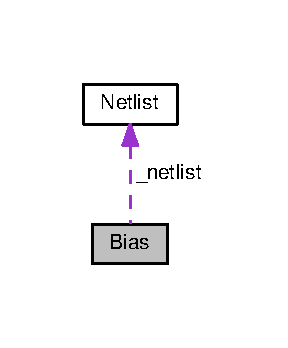
\includegraphics[width=138pt]{classBias__coll__graph}
\end{center}
\end{figure}
\subsection*{Public Member Functions}
\begin{DoxyCompactItemize}
\item 
\hyperlink{classBias_a5e0a80d4549e61f0e5d8c9d00659ad4d}{Bias} ()=default
\begin{DoxyCompactList}\small\item\em Default Constructor. \end{DoxyCompactList}\item 
\hyperlink{classBias_a1373ea9210307ff6e856d705ca24cd1d}{Bias} (\hyperlink{type_8h_a581e8093e28e7362f2b6937296190676}{Index\+Type} net\+Id, const \hyperlink{classNetlist}{Netlist} \&netlist)
\begin{DoxyCompactList}\small\item\em Constructor for \hyperlink{classBias}{Bias}. \end{DoxyCompactList}\item 
const std\+::vector$<$ \hyperlink{type_8h_a581e8093e28e7362f2b6937296190676}{Index\+Type} $>$ \& \hyperlink{classBias_ae8bea9924068867c86a28fa01fe015dc}{bias} () const
\begin{DoxyCompactList}\small\item\em Get entire bias group. \end{DoxyCompactList}\item 
const std\+::vector$<$ \hyperlink{type_8h_a581e8093e28e7362f2b6937296190676}{Index\+Type} $>$ \& \hyperlink{classBias_a1ce69bcc1c78a3a06ba13a3bcb363fb5}{driver} () const
\begin{DoxyCompactList}\small\item\em Get the driver group. \end{DoxyCompactList}\item 
bool \hyperlink{classBias_ae917e3b0f32f52639db370bc49766328}{valid} () const
\item 
void \hyperlink{classBias_ab2453141710ffdb4644d6427c3edd34d}{init} ()
\end{DoxyCompactItemize}
\subsection*{Private Attributes}
\begin{DoxyCompactItemize}
\item 
\hyperlink{type_8h_a581e8093e28e7362f2b6937296190676}{Index\+Type} \hyperlink{classBias_a9fac526ba276c7593241f7ba439c0f31}{\+\_\+net\+Id}
\item 
const \hyperlink{classNetlist}{Netlist} \& \hyperlink{classBias_a80d38b13e72f5586c72013a91f6914a6}{\+\_\+netlist}
\item 
std\+::vector$<$ \hyperlink{type_8h_a581e8093e28e7362f2b6937296190676}{Index\+Type} $>$ \hyperlink{classBias_a8b24bf7291399bf389c9c73d585a02f2}{\+\_\+bias}
\item 
std\+::vector$<$ \hyperlink{type_8h_a581e8093e28e7362f2b6937296190676}{Index\+Type} $>$ \hyperlink{classBias_a51db005f686c23b55031be0e6daf3fdd}{\+\_\+driver}
\end{DoxyCompactItemize}


\subsection{Detailed Description}
A vector of Mosfet. 

This class stores a group of Mosfet Id that are bias circuits. 

\subsection{Constructor \& Destructor Documentation}
\mbox{\Hypertarget{classBias_a5e0a80d4549e61f0e5d8c9d00659ad4d}\label{classBias_a5e0a80d4549e61f0e5d8c9d00659ad4d}} 
\index{Bias@{Bias}!Bias@{Bias}}
\index{Bias@{Bias}!Bias@{Bias}}
\subsubsection{\texorpdfstring{Bias()}{Bias()}\hspace{0.1cm}{\footnotesize\ttfamily [1/2]}}
{\footnotesize\ttfamily Bias\+::\+Bias (\begin{DoxyParamCaption}{ }\end{DoxyParamCaption})\hspace{0.3cm}{\ttfamily [explicit]}, {\ttfamily [default]}}



Default Constructor. 

\mbox{\Hypertarget{classBias_a1373ea9210307ff6e856d705ca24cd1d}\label{classBias_a1373ea9210307ff6e856d705ca24cd1d}} 
\index{Bias@{Bias}!Bias@{Bias}}
\index{Bias@{Bias}!Bias@{Bias}}
\subsubsection{\texorpdfstring{Bias()}{Bias()}\hspace{0.1cm}{\footnotesize\ttfamily [2/2]}}
{\footnotesize\ttfamily Bias\+::\+Bias (\begin{DoxyParamCaption}\item[{\hyperlink{type_8h_a581e8093e28e7362f2b6937296190676}{Index\+Type}}]{net\+Id,  }\item[{const \hyperlink{classNetlist}{Netlist} \&}]{netlist }\end{DoxyParamCaption})\hspace{0.3cm}{\ttfamily [inline]}, {\ttfamily [explicit]}}



Constructor for \hyperlink{classBias}{Bias}. 

Sequence of Ids does not matter. pattern is set according to input.


\begin{DoxyParams}{Parameters}
{\em net\+Id} & Gate net\+Id. \\
\hline
{\em netlist} & \hyperlink{classNetlist}{Netlist} class object. \\
\hline
\end{DoxyParams}


\subsection{Member Function Documentation}
\mbox{\Hypertarget{classBias_ae8bea9924068867c86a28fa01fe015dc}\label{classBias_ae8bea9924068867c86a28fa01fe015dc}} 
\index{Bias@{Bias}!bias@{bias}}
\index{bias@{bias}!Bias@{Bias}}
\subsubsection{\texorpdfstring{bias()}{bias()}}
{\footnotesize\ttfamily const std\+::vector$<$\hyperlink{type_8h_a581e8093e28e7362f2b6937296190676}{Index\+Type}$>$\& Bias\+::bias (\begin{DoxyParamCaption}{ }\end{DoxyParamCaption}) const\hspace{0.3cm}{\ttfamily [inline]}}



Get entire bias group. 

\mbox{\Hypertarget{classBias_a1ce69bcc1c78a3a06ba13a3bcb363fb5}\label{classBias_a1ce69bcc1c78a3a06ba13a3bcb363fb5}} 
\index{Bias@{Bias}!driver@{driver}}
\index{driver@{driver}!Bias@{Bias}}
\subsubsection{\texorpdfstring{driver()}{driver()}}
{\footnotesize\ttfamily const std\+::vector$<$\hyperlink{type_8h_a581e8093e28e7362f2b6937296190676}{Index\+Type}$>$\& Bias\+::driver (\begin{DoxyParamCaption}{ }\end{DoxyParamCaption}) const\hspace{0.3cm}{\ttfamily [inline]}}



Get the driver group. 

\mbox{\Hypertarget{classBias_ab2453141710ffdb4644d6427c3edd34d}\label{classBias_ab2453141710ffdb4644d6427c3edd34d}} 
\index{Bias@{Bias}!init@{init}}
\index{init@{init}!Bias@{Bias}}
\subsubsection{\texorpdfstring{init()}{init()}}
{\footnotesize\ttfamily \hyperlink{namespace_8h_ae48726a24dab2034454cf6d79e531eb8}{P\+R\+O\+J\+E\+C\+T\+\_\+\+N\+A\+M\+E\+S\+P\+A\+C\+E\+\_\+\+B\+E\+G\+IN} void Bias\+::init (\begin{DoxyParamCaption}{ }\end{DoxyParamCaption})}

\mbox{\Hypertarget{classBias_ae917e3b0f32f52639db370bc49766328}\label{classBias_ae917e3b0f32f52639db370bc49766328}} 
\index{Bias@{Bias}!valid@{valid}}
\index{valid@{valid}!Bias@{Bias}}
\subsubsection{\texorpdfstring{valid()}{valid()}}
{\footnotesize\ttfamily bool Bias\+::valid (\begin{DoxyParamCaption}{ }\end{DoxyParamCaption}) const\hspace{0.3cm}{\ttfamily [inline]}}



\subsection{Member Data Documentation}
\mbox{\Hypertarget{classBias_a8b24bf7291399bf389c9c73d585a02f2}\label{classBias_a8b24bf7291399bf389c9c73d585a02f2}} 
\index{Bias@{Bias}!\+\_\+bias@{\+\_\+bias}}
\index{\+\_\+bias@{\+\_\+bias}!Bias@{Bias}}
\subsubsection{\texorpdfstring{\+\_\+bias}{\_bias}}
{\footnotesize\ttfamily std\+::vector$<$\hyperlink{type_8h_a581e8093e28e7362f2b6937296190676}{Index\+Type}$>$ Bias\+::\+\_\+bias\hspace{0.3cm}{\ttfamily [private]}}

\mbox{\Hypertarget{classBias_a51db005f686c23b55031be0e6daf3fdd}\label{classBias_a51db005f686c23b55031be0e6daf3fdd}} 
\index{Bias@{Bias}!\+\_\+driver@{\+\_\+driver}}
\index{\+\_\+driver@{\+\_\+driver}!Bias@{Bias}}
\subsubsection{\texorpdfstring{\+\_\+driver}{\_driver}}
{\footnotesize\ttfamily std\+::vector$<$\hyperlink{type_8h_a581e8093e28e7362f2b6937296190676}{Index\+Type}$>$ Bias\+::\+\_\+driver\hspace{0.3cm}{\ttfamily [private]}}

\mbox{\Hypertarget{classBias_a9fac526ba276c7593241f7ba439c0f31}\label{classBias_a9fac526ba276c7593241f7ba439c0f31}} 
\index{Bias@{Bias}!\+\_\+net\+Id@{\+\_\+net\+Id}}
\index{\+\_\+net\+Id@{\+\_\+net\+Id}!Bias@{Bias}}
\subsubsection{\texorpdfstring{\+\_\+net\+Id}{\_netId}}
{\footnotesize\ttfamily \hyperlink{type_8h_a581e8093e28e7362f2b6937296190676}{Index\+Type} Bias\+::\+\_\+net\+Id\hspace{0.3cm}{\ttfamily [private]}}

\mbox{\Hypertarget{classBias_a80d38b13e72f5586c72013a91f6914a6}\label{classBias_a80d38b13e72f5586c72013a91f6914a6}} 
\index{Bias@{Bias}!\+\_\+netlist@{\+\_\+netlist}}
\index{\+\_\+netlist@{\+\_\+netlist}!Bias@{Bias}}
\subsubsection{\texorpdfstring{\+\_\+netlist}{\_netlist}}
{\footnotesize\ttfamily const \hyperlink{classNetlist}{Netlist}\& Bias\+::\+\_\+netlist\hspace{0.3cm}{\ttfamily [private]}}



The documentation for this class was generated from the following files\+:\begin{DoxyCompactItemize}
\item 
src/db/\hyperlink{Bias_8h}{Bias.\+h}\item 
src/db/\hyperlink{Bias_8cpp}{Bias.\+cpp}\end{DoxyCompactItemize}

\hypertarget{structNetlist_1_1InitDataObj}{}\section{Netlist\+:\+:Init\+Data\+Obj Struct Reference}
\label{structNetlist_1_1InitDataObj}\index{Netlist\+::\+Init\+Data\+Obj@{Netlist\+::\+Init\+Data\+Obj}}


Instantiate \hyperlink{classNetlist}{Netlist} class.  




{\ttfamily \#include $<$Netlist.\+h$>$}

\subsection*{Public Attributes}
\begin{DoxyCompactItemize}
\item 
std\+::vector$<$ \hyperlink{structNetlist_1_1InitNet}{Init\+Net} $>$ \hyperlink{structNetlist_1_1InitDataObj_a6da3cc62735730affa77954952d1f217}{net\+Array}
\item 
std\+::vector$<$ \hyperlink{structNetlist_1_1InitInst}{Init\+Inst} $>$ \hyperlink{structNetlist_1_1InitDataObj_af268c80f194c76f372f8e1dbaed071e0}{inst\+Array}
\end{DoxyCompactItemize}


\subsection{Detailed Description}
Instantiate \hyperlink{classNetlist}{Netlist} class. 

\begin{DoxySeeAlso}{See also}
\hyperlink{classNetlist_ab61cbc31bee838b90f29c52aaae1e52a}{init(\+Init\+Data\+Obj \&)}. 
\end{DoxySeeAlso}


\subsection{Member Data Documentation}
\mbox{\Hypertarget{structNetlist_1_1InitDataObj_af268c80f194c76f372f8e1dbaed071e0}\label{structNetlist_1_1InitDataObj_af268c80f194c76f372f8e1dbaed071e0}} 
\index{Netlist\+::\+Init\+Data\+Obj@{Netlist\+::\+Init\+Data\+Obj}!inst\+Array@{inst\+Array}}
\index{inst\+Array@{inst\+Array}!Netlist\+::\+Init\+Data\+Obj@{Netlist\+::\+Init\+Data\+Obj}}
\subsubsection{\texorpdfstring{inst\+Array}{instArray}}
{\footnotesize\ttfamily std\+::vector$<$\hyperlink{structNetlist_1_1InitInst}{Init\+Inst}$>$ Netlist\+::\+Init\+Data\+Obj\+::inst\+Array}

\mbox{\Hypertarget{structNetlist_1_1InitDataObj_a6da3cc62735730affa77954952d1f217}\label{structNetlist_1_1InitDataObj_a6da3cc62735730affa77954952d1f217}} 
\index{Netlist\+::\+Init\+Data\+Obj@{Netlist\+::\+Init\+Data\+Obj}!net\+Array@{net\+Array}}
\index{net\+Array@{net\+Array}!Netlist\+::\+Init\+Data\+Obj@{Netlist\+::\+Init\+Data\+Obj}}
\subsubsection{\texorpdfstring{net\+Array}{netArray}}
{\footnotesize\ttfamily std\+::vector$<$\hyperlink{structNetlist_1_1InitNet}{Init\+Net}$>$ Netlist\+::\+Init\+Data\+Obj\+::net\+Array}



The documentation for this struct was generated from the following file\+:\begin{DoxyCompactItemize}
\item 
src/db/\hyperlink{Netlist_8h}{Netlist.\+h}\end{DoxyCompactItemize}

\hypertarget{structNetlist_1_1InitInst}{}\section{Netlist\+:\+:Init\+Inst Struct Reference}
\label{structNetlist_1_1InitInst}\index{Netlist\+::\+Init\+Inst@{Netlist\+::\+Init\+Inst}}


\hyperlink{classInst}{Inst} for instantiation.  




{\ttfamily \#include $<$Netlist.\+h$>$}

\subsection*{Public Attributes}
\begin{DoxyCompactItemize}
\item 
\hyperlink{type_8h_a53644c687d6bc203d9d3d3ee70075f61}{Inst\+Type} \hyperlink{structNetlist_1_1InitInst_a19eaae603a2805874691d6942e0e3400}{type} = \hyperlink{type_8h_a53644c687d6bc203d9d3d3ee70075f61a03570470bad94692ce93e32700d2e1cb}{Inst\+Type\+::\+O\+T\+H\+ER}
\item 
std\+::vector$<$ \hyperlink{type_8h_a581e8093e28e7362f2b6937296190676}{Index\+Type} $>$ \hyperlink{structNetlist_1_1InitInst_a0c1130b16eee45cc956cbff8d989c581}{net\+Id\+Array}
\item 
std\+::string \hyperlink{structNetlist_1_1InitInst_ab15aa94aa397cb0affe046473bf592e6}{name}
\item 
\hyperlink{type_8h_a51898ad9e46b1265f3fab67f7d4b04a2}{Real\+Type} \hyperlink{structNetlist_1_1InitInst_ab330bc688ba619aae2f1e2b64599f6e8}{wid} = 0
\item 
\hyperlink{type_8h_a51898ad9e46b1265f3fab67f7d4b04a2}{Real\+Type} \hyperlink{structNetlist_1_1InitInst_a913df6563e26da7c753db4c0bf7834b4}{len} = 0
\end{DoxyCompactItemize}


\subsection{Detailed Description}
\hyperlink{classInst}{Inst} for instantiation. 

\subsection{Member Data Documentation}
\mbox{\Hypertarget{structNetlist_1_1InitInst_a913df6563e26da7c753db4c0bf7834b4}\label{structNetlist_1_1InitInst_a913df6563e26da7c753db4c0bf7834b4}} 
\index{Netlist\+::\+Init\+Inst@{Netlist\+::\+Init\+Inst}!len@{len}}
\index{len@{len}!Netlist\+::\+Init\+Inst@{Netlist\+::\+Init\+Inst}}
\subsubsection{\texorpdfstring{len}{len}}
{\footnotesize\ttfamily \hyperlink{type_8h_a51898ad9e46b1265f3fab67f7d4b04a2}{Real\+Type} Netlist\+::\+Init\+Inst\+::len = 0}

\mbox{\Hypertarget{structNetlist_1_1InitInst_ab15aa94aa397cb0affe046473bf592e6}\label{structNetlist_1_1InitInst_ab15aa94aa397cb0affe046473bf592e6}} 
\index{Netlist\+::\+Init\+Inst@{Netlist\+::\+Init\+Inst}!name@{name}}
\index{name@{name}!Netlist\+::\+Init\+Inst@{Netlist\+::\+Init\+Inst}}
\subsubsection{\texorpdfstring{name}{name}}
{\footnotesize\ttfamily std\+::string Netlist\+::\+Init\+Inst\+::name}

\mbox{\Hypertarget{structNetlist_1_1InitInst_a0c1130b16eee45cc956cbff8d989c581}\label{structNetlist_1_1InitInst_a0c1130b16eee45cc956cbff8d989c581}} 
\index{Netlist\+::\+Init\+Inst@{Netlist\+::\+Init\+Inst}!net\+Id\+Array@{net\+Id\+Array}}
\index{net\+Id\+Array@{net\+Id\+Array}!Netlist\+::\+Init\+Inst@{Netlist\+::\+Init\+Inst}}
\subsubsection{\texorpdfstring{net\+Id\+Array}{netIdArray}}
{\footnotesize\ttfamily std\+::vector$<$\hyperlink{type_8h_a581e8093e28e7362f2b6937296190676}{Index\+Type}$>$ Netlist\+::\+Init\+Inst\+::net\+Id\+Array}

\mbox{\Hypertarget{structNetlist_1_1InitInst_a19eaae603a2805874691d6942e0e3400}\label{structNetlist_1_1InitInst_a19eaae603a2805874691d6942e0e3400}} 
\index{Netlist\+::\+Init\+Inst@{Netlist\+::\+Init\+Inst}!type@{type}}
\index{type@{type}!Netlist\+::\+Init\+Inst@{Netlist\+::\+Init\+Inst}}
\subsubsection{\texorpdfstring{type}{type}}
{\footnotesize\ttfamily \hyperlink{type_8h_a53644c687d6bc203d9d3d3ee70075f61}{Inst\+Type} Netlist\+::\+Init\+Inst\+::type = \hyperlink{type_8h_a53644c687d6bc203d9d3d3ee70075f61a03570470bad94692ce93e32700d2e1cb}{Inst\+Type\+::\+O\+T\+H\+ER}}

\mbox{\Hypertarget{structNetlist_1_1InitInst_ab330bc688ba619aae2f1e2b64599f6e8}\label{structNetlist_1_1InitInst_ab330bc688ba619aae2f1e2b64599f6e8}} 
\index{Netlist\+::\+Init\+Inst@{Netlist\+::\+Init\+Inst}!wid@{wid}}
\index{wid@{wid}!Netlist\+::\+Init\+Inst@{Netlist\+::\+Init\+Inst}}
\subsubsection{\texorpdfstring{wid}{wid}}
{\footnotesize\ttfamily \hyperlink{type_8h_a51898ad9e46b1265f3fab67f7d4b04a2}{Real\+Type} Netlist\+::\+Init\+Inst\+::wid = 0}



The documentation for this struct was generated from the following file\+:\begin{DoxyCompactItemize}
\item 
src/db/\hyperlink{Netlist_8h}{Netlist.\+h}\end{DoxyCompactItemize}

\hypertarget{structNetlist_1_1InitNet}{}\section{Netlist\+:\+:Init\+Net Struct Reference}
\label{structNetlist_1_1InitNet}\index{Netlist\+::\+Init\+Net@{Netlist\+::\+Init\+Net}}


\hyperlink{classNet}{Net} for instantiation.  




{\ttfamily \#include $<$Netlist.\+h$>$}

\subsection*{Public Attributes}
\begin{DoxyCompactItemize}
\item 
std\+::string \hyperlink{structNetlist_1_1InitNet_acb4d378b948bc8e2cd1490f62683ed2d}{name}
\item 
\hyperlink{type_8h_a581e8093e28e7362f2b6937296190676}{Index\+Type} \hyperlink{structNetlist_1_1InitNet_a26ea0dea8ddabe80a0edbb60cd422dcc}{id} = \hyperlink{type_8h_a11591ec4ef05af2b0f48545966a61500}{I\+N\+D\+E\+X\+\_\+\+T\+Y\+P\+E\+\_\+\+M\+AX}
\end{DoxyCompactItemize}


\subsection{Detailed Description}
\hyperlink{classNet}{Net} for instantiation. 

\subsection{Member Data Documentation}
\mbox{\Hypertarget{structNetlist_1_1InitNet_a26ea0dea8ddabe80a0edbb60cd422dcc}\label{structNetlist_1_1InitNet_a26ea0dea8ddabe80a0edbb60cd422dcc}} 
\index{Netlist\+::\+Init\+Net@{Netlist\+::\+Init\+Net}!id@{id}}
\index{id@{id}!Netlist\+::\+Init\+Net@{Netlist\+::\+Init\+Net}}
\subsubsection{\texorpdfstring{id}{id}}
{\footnotesize\ttfamily \hyperlink{type_8h_a581e8093e28e7362f2b6937296190676}{Index\+Type} Netlist\+::\+Init\+Net\+::id = \hyperlink{type_8h_a11591ec4ef05af2b0f48545966a61500}{I\+N\+D\+E\+X\+\_\+\+T\+Y\+P\+E\+\_\+\+M\+AX}}

\mbox{\Hypertarget{structNetlist_1_1InitNet_acb4d378b948bc8e2cd1490f62683ed2d}\label{structNetlist_1_1InitNet_acb4d378b948bc8e2cd1490f62683ed2d}} 
\index{Netlist\+::\+Init\+Net@{Netlist\+::\+Init\+Net}!name@{name}}
\index{name@{name}!Netlist\+::\+Init\+Net@{Netlist\+::\+Init\+Net}}
\subsubsection{\texorpdfstring{name}{name}}
{\footnotesize\ttfamily std\+::string Netlist\+::\+Init\+Net\+::name}



The documentation for this struct was generated from the following file\+:\begin{DoxyCompactItemize}
\item 
src/db/\hyperlink{Netlist_8h}{Netlist.\+h}\end{DoxyCompactItemize}

\hypertarget{classInitNetlist}{}\section{Init\+Netlist Class Reference}
\label{classInitNetlist}\index{Init\+Netlist@{Init\+Netlist}}


\hyperlink{classInitNetlist}{Init\+Netlist} class.  




{\ttfamily \#include $<$Init\+Netlist.\+h$>$}



Collaboration diagram for Init\+Netlist\+:\nopagebreak
\begin{figure}[H]
\begin{center}
\leavevmode
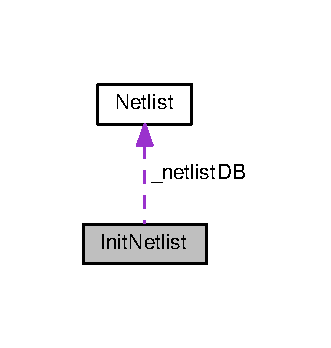
\includegraphics[width=159pt]{classInitNetlist__coll__graph}
\end{center}
\end{figure}
\subsection*{Public Member Functions}
\begin{DoxyCompactItemize}
\item 
\hyperlink{classInitNetlist_a9def85cc1861a8a74494d9fd494acdeb}{Init\+Netlist} ()=default
\begin{DoxyCompactList}\small\item\em Default Constructor. \end{DoxyCompactList}\item 
\hyperlink{classInitNetlist_a330ee469b31e43357171f5943dad6387}{Init\+Netlist} (\hyperlink{classNetlist}{Netlist} \&netlist)
\begin{DoxyCompactList}\small\item\em Constructor with initialization. \end{DoxyCompactList}\item 
bool \hyperlink{classInitNetlist_a4c173b7e51678aad9937969e2e54f867}{read} (const std\+::string \&filename)
\begin{DoxyCompactList}\small\item\em Parse file and build netlist. \end{DoxyCompactList}\end{DoxyCompactItemize}
\subsection*{Private Attributes}
\begin{DoxyCompactItemize}
\item 
\hyperlink{classNetlist}{Netlist} \& \hyperlink{classInitNetlist_af6a6b4238c1ecfeebfa3344426647743}{\+\_\+netlist\+DB}
\end{DoxyCompactItemize}


\subsection{Detailed Description}
\hyperlink{classInitNetlist}{Init\+Netlist} class. 

\subsection{Constructor \& Destructor Documentation}
\mbox{\Hypertarget{classInitNetlist_a9def85cc1861a8a74494d9fd494acdeb}\label{classInitNetlist_a9def85cc1861a8a74494d9fd494acdeb}} 
\index{Init\+Netlist@{Init\+Netlist}!Init\+Netlist@{Init\+Netlist}}
\index{Init\+Netlist@{Init\+Netlist}!Init\+Netlist@{Init\+Netlist}}
\subsubsection{\texorpdfstring{Init\+Netlist()}{InitNetlist()}\hspace{0.1cm}{\footnotesize\ttfamily [1/2]}}
{\footnotesize\ttfamily Init\+Netlist\+::\+Init\+Netlist (\begin{DoxyParamCaption}{ }\end{DoxyParamCaption})\hspace{0.3cm}{\ttfamily [explicit]}, {\ttfamily [default]}}



Default Constructor. 

\mbox{\Hypertarget{classInitNetlist_a330ee469b31e43357171f5943dad6387}\label{classInitNetlist_a330ee469b31e43357171f5943dad6387}} 
\index{Init\+Netlist@{Init\+Netlist}!Init\+Netlist@{Init\+Netlist}}
\index{Init\+Netlist@{Init\+Netlist}!Init\+Netlist@{Init\+Netlist}}
\subsubsection{\texorpdfstring{Init\+Netlist()}{InitNetlist()}\hspace{0.1cm}{\footnotesize\ttfamily [2/2]}}
{\footnotesize\ttfamily Init\+Netlist\+::\+Init\+Netlist (\begin{DoxyParamCaption}\item[{\hyperlink{classNetlist}{Netlist} \&}]{netlist }\end{DoxyParamCaption})\hspace{0.3cm}{\ttfamily [inline]}, {\ttfamily [explicit]}}



Constructor with initialization. 



\subsection{Member Function Documentation}
\mbox{\Hypertarget{classInitNetlist_a4c173b7e51678aad9937969e2e54f867}\label{classInitNetlist_a4c173b7e51678aad9937969e2e54f867}} 
\index{Init\+Netlist@{Init\+Netlist}!read@{read}}
\index{read@{read}!Init\+Netlist@{Init\+Netlist}}
\subsubsection{\texorpdfstring{read()}{read()}}
{\footnotesize\ttfamily \hyperlink{namespace_8h_ae48726a24dab2034454cf6d79e531eb8}{P\+R\+O\+J\+E\+C\+T\+\_\+\+N\+A\+M\+E\+S\+P\+A\+C\+E\+\_\+\+B\+E\+G\+IN} bool Init\+Netlist\+::read (\begin{DoxyParamCaption}\item[{const std\+::string \&}]{filename }\end{DoxyParamCaption})}



Parse file and build netlist. 

Input files should follow same format generated through scripts/create\+\_\+init\+\_\+obj.\+py. Sample input files for c++ are under benchmarks. The python scripts take standardized hspice/spectre netlist files as inputs.


\begin{DoxyParams}{Parameters}
{\em filename} & Input file to parse. \\
\hline
\end{DoxyParams}


\subsection{Member Data Documentation}
\mbox{\Hypertarget{classInitNetlist_af6a6b4238c1ecfeebfa3344426647743}\label{classInitNetlist_af6a6b4238c1ecfeebfa3344426647743}} 
\index{Init\+Netlist@{Init\+Netlist}!\+\_\+netlist\+DB@{\+\_\+netlist\+DB}}
\index{\+\_\+netlist\+DB@{\+\_\+netlist\+DB}!Init\+Netlist@{Init\+Netlist}}
\subsubsection{\texorpdfstring{\+\_\+netlist\+DB}{\_netlistDB}}
{\footnotesize\ttfamily \hyperlink{classNetlist}{Netlist}\& Init\+Netlist\+::\+\_\+netlist\+DB\hspace{0.3cm}{\ttfamily [private]}}



The documentation for this class was generated from the following files\+:\begin{DoxyCompactItemize}
\item 
src/parser/\hyperlink{InitNetlist_8h}{Init\+Netlist.\+h}\item 
src/parser/\hyperlink{InitNetlist_8cpp}{Init\+Netlist.\+cpp}\end{DoxyCompactItemize}

\hypertarget{classInst}{}\section{Inst Class Reference}
\label{classInst}\index{Inst@{Inst}}


\hyperlink{classInst}{Inst} class.  




{\ttfamily \#include $<$Inst.\+h$>$}

\subsection*{Public Member Functions}
\begin{DoxyCompactItemize}
\item 
\hyperlink{classInst_af6abd595ee04b976a8928325df4076c1}{Inst} ()=default
\begin{DoxyCompactList}\small\item\em Default constructor. \end{DoxyCompactList}\item 
\hyperlink{classInst_a30315ac6216ae022a383d701d42e6a86}{Inst} (const std\+::string \&\hyperlink{classInst_af2eca464fb81066a6f9878ae24a8292a}{name}, \hyperlink{type_8h_a53644c687d6bc203d9d3d3ee70075f61}{Inst\+Type} \hyperlink{classInst_a7d6e3dafcbb552bf31069d80b9b87607}{type}, \hyperlink{type_8h_a581e8093e28e7362f2b6937296190676}{Index\+Type} \hyperlink{classInst_a42b641ca923af69de223b8911cc2d45f}{id})
\begin{DoxyCompactList}\small\item\em Constructor for \hyperlink{classInst}{Inst}. \end{DoxyCompactList}\item 
\hyperlink{classInst_adb54d3441f94302e5d0c8e0d8c3ad429}{Inst} (const std\+::string \&\hyperlink{classInst_af2eca464fb81066a6f9878ae24a8292a}{name}, \hyperlink{type_8h_a53644c687d6bc203d9d3d3ee70075f61}{Inst\+Type} \hyperlink{classInst_a7d6e3dafcbb552bf31069d80b9b87607}{type}, \hyperlink{type_8h_a581e8093e28e7362f2b6937296190676}{Index\+Type} \hyperlink{classInst_a42b641ca923af69de223b8911cc2d45f}{id}, \hyperlink{type_8h_a51898ad9e46b1265f3fab67f7d4b04a2}{Real\+Type} \hyperlink{classInst_a18cd79f2cb3e30b1d8731381d311a919}{wid}, \hyperlink{type_8h_a51898ad9e46b1265f3fab67f7d4b04a2}{Real\+Type} \hyperlink{classInst_ab90470caf2f50b7127ee6946d93d449e}{len})
\begin{DoxyCompactList}\small\item\em Constructor for \hyperlink{classInst}{Inst}. \end{DoxyCompactList}\item 
const std\+::string \& \hyperlink{classInst_af2eca464fb81066a6f9878ae24a8292a}{name} () const
\item 
\hyperlink{type_8h_a53644c687d6bc203d9d3d3ee70075f61}{Inst\+Type} \hyperlink{classInst_a7d6e3dafcbb552bf31069d80b9b87607}{type} () const
\begin{DoxyCompactList}\small\item\em Return type of \hyperlink{classInst}{Inst}. \end{DoxyCompactList}\item 
\hyperlink{type_8h_a581e8093e28e7362f2b6937296190676}{Index\+Type} \hyperlink{classInst_a42b641ca923af69de223b8911cc2d45f}{id} () const
\begin{DoxyCompactList}\small\item\em Return Id of \hyperlink{classInst}{Inst}. \end{DoxyCompactList}\item 
const std\+::vector$<$ \hyperlink{type_8h_a581e8093e28e7362f2b6937296190676}{Index\+Type} $>$ \& \hyperlink{classInst_ab63305e9b98c220c6c09b8d69a8c8a71}{pin\+Id\+Array} () const
\begin{DoxyCompactList}\small\item\em Return the index array for pins of the \hyperlink{classInst}{Inst}. \end{DoxyCompactList}\item 
\hyperlink{type_8h_a51898ad9e46b1265f3fab67f7d4b04a2}{Real\+Type} \hyperlink{classInst_a18cd79f2cb3e30b1d8731381d311a919}{wid} () const
\begin{DoxyCompactList}\small\item\em Return width of \hyperlink{classInst}{Inst}. \end{DoxyCompactList}\item 
\hyperlink{type_8h_a51898ad9e46b1265f3fab67f7d4b04a2}{Real\+Type} \hyperlink{classInst_ab90470caf2f50b7127ee6946d93d449e}{len} () const
\begin{DoxyCompactList}\small\item\em Return length of \hyperlink{classInst}{Inst}. \end{DoxyCompactList}\item 
void \hyperlink{classInst_afee7f1349599a3514f0c6b0613ce9656}{add\+Pin\+Id} (\hyperlink{type_8h_a581e8093e28e7362f2b6937296190676}{Index\+Type} pin\+Id)
\begin{DoxyCompactList}\small\item\em Add pin index to \hyperlink{classInst}{Inst}. \end{DoxyCompactList}\item 
void \hyperlink{classInst_a0667cb5b7b7ef52c67ce0f2514b933b0}{set\+Wid} (\hyperlink{type_8h_a51898ad9e46b1265f3fab67f7d4b04a2}{Real\+Type} \hyperlink{classInst_a18cd79f2cb3e30b1d8731381d311a919}{wid})
\begin{DoxyCompactList}\small\item\em Assign width of \hyperlink{classInst}{Inst}. \end{DoxyCompactList}\item 
void \hyperlink{classInst_a63908bff80f6af5034e6d51e894a54e2}{set\+Len} (\hyperlink{type_8h_a51898ad9e46b1265f3fab67f7d4b04a2}{Real\+Type} \hyperlink{classInst_ab90470caf2f50b7127ee6946d93d449e}{len})
\begin{DoxyCompactList}\small\item\em Assign length of \hyperlink{classInst}{Inst}. \end{DoxyCompactList}\end{DoxyCompactItemize}
\subsection*{Private Attributes}
\begin{DoxyCompactItemize}
\item 
std\+::string \hyperlink{classInst_a2f11b1c4d2151470182e0d24f7bddbbb}{\+\_\+name}
\item 
\hyperlink{type_8h_a53644c687d6bc203d9d3d3ee70075f61}{Inst\+Type} \hyperlink{classInst_a71f59c0ab13351f33a67c57839aa5e3d}{\+\_\+type}
\item 
\hyperlink{type_8h_a581e8093e28e7362f2b6937296190676}{Index\+Type} \hyperlink{classInst_a11c7c07b99b2a60e9637a3a1a67911e5}{\+\_\+id}
\item 
std\+::vector$<$ \hyperlink{type_8h_a581e8093e28e7362f2b6937296190676}{Index\+Type} $>$ \hyperlink{classInst_aba5f13fac393f1f506630ef1259853b7}{\+\_\+pin\+Id\+Array}
\item 
\hyperlink{type_8h_a51898ad9e46b1265f3fab67f7d4b04a2}{Real\+Type} \hyperlink{classInst_ad9ded5bad369f4ab225372c839820ab9}{\+\_\+wid}
\item 
\hyperlink{type_8h_a51898ad9e46b1265f3fab67f7d4b04a2}{Real\+Type} \hyperlink{classInst_acb3bddc4216dba958466c34fb5698adc}{\+\_\+len}
\end{DoxyCompactItemize}


\subsection{Detailed Description}
\hyperlink{classInst}{Inst} class. 

\subsection{Constructor \& Destructor Documentation}
\mbox{\Hypertarget{classInst_af6abd595ee04b976a8928325df4076c1}\label{classInst_af6abd595ee04b976a8928325df4076c1}} 
\index{Inst@{Inst}!Inst@{Inst}}
\index{Inst@{Inst}!Inst@{Inst}}
\subsubsection{\texorpdfstring{Inst()}{Inst()}\hspace{0.1cm}{\footnotesize\ttfamily [1/3]}}
{\footnotesize\ttfamily Inst\+::\+Inst (\begin{DoxyParamCaption}{ }\end{DoxyParamCaption})\hspace{0.3cm}{\ttfamily [explicit]}, {\ttfamily [default]}}



Default constructor. 

\mbox{\Hypertarget{classInst_a30315ac6216ae022a383d701d42e6a86}\label{classInst_a30315ac6216ae022a383d701d42e6a86}} 
\index{Inst@{Inst}!Inst@{Inst}}
\index{Inst@{Inst}!Inst@{Inst}}
\subsubsection{\texorpdfstring{Inst()}{Inst()}\hspace{0.1cm}{\footnotesize\ttfamily [2/3]}}
{\footnotesize\ttfamily Inst\+::\+Inst (\begin{DoxyParamCaption}\item[{const std\+::string \&}]{name,  }\item[{\hyperlink{type_8h_a53644c687d6bc203d9d3d3ee70075f61}{Inst\+Type}}]{type,  }\item[{\hyperlink{type_8h_a581e8093e28e7362f2b6937296190676}{Index\+Type}}]{id }\end{DoxyParamCaption})\hspace{0.3cm}{\ttfamily [inline]}, {\ttfamily [explicit]}}



Constructor for \hyperlink{classInst}{Inst}. 

Constructor for netlist instances that does not have width and length attributes.


\begin{DoxyParams}{Parameters}
{\em name} & Name of \hyperlink{classInst}{Inst}. \\
\hline
{\em type} & Type of \hyperlink{classInst}{Inst}. Member of Inst\+Type. \\
\hline
\end{DoxyParams}
\begin{DoxySeeAlso}{See also}
\hyperlink{type_8h}{type.\+h} 
\end{DoxySeeAlso}

\begin{DoxyParams}{Parameters}
{\em id} & Id of \hyperlink{classInst}{Inst}. \\
\hline
\end{DoxyParams}
\mbox{\Hypertarget{classInst_adb54d3441f94302e5d0c8e0d8c3ad429}\label{classInst_adb54d3441f94302e5d0c8e0d8c3ad429}} 
\index{Inst@{Inst}!Inst@{Inst}}
\index{Inst@{Inst}!Inst@{Inst}}
\subsubsection{\texorpdfstring{Inst()}{Inst()}\hspace{0.1cm}{\footnotesize\ttfamily [3/3]}}
{\footnotesize\ttfamily Inst\+::\+Inst (\begin{DoxyParamCaption}\item[{const std\+::string \&}]{name,  }\item[{\hyperlink{type_8h_a53644c687d6bc203d9d3d3ee70075f61}{Inst\+Type}}]{type,  }\item[{\hyperlink{type_8h_a581e8093e28e7362f2b6937296190676}{Index\+Type}}]{id,  }\item[{\hyperlink{type_8h_a51898ad9e46b1265f3fab67f7d4b04a2}{Real\+Type}}]{wid,  }\item[{\hyperlink{type_8h_a51898ad9e46b1265f3fab67f7d4b04a2}{Real\+Type}}]{len }\end{DoxyParamCaption})\hspace{0.3cm}{\ttfamily [inline]}, {\ttfamily [explicit]}}



Constructor for \hyperlink{classInst}{Inst}. 

Constructor for netlist instances that have width and length attributes.


\begin{DoxyParams}{Parameters}
{\em name} & Name of \hyperlink{classInst}{Inst}. \\
\hline
{\em type} & Type of \hyperlink{classInst}{Inst}. Member of Inst\+Type. \\
\hline
{\em id} & Id of I\+Nst. \\
\hline
{\em wid} & Width of \hyperlink{classInst}{Inst}. \\
\hline
{\em len} & Length of \hyperlink{classInst}{Inst}. \\
\hline
\end{DoxyParams}


\subsection{Member Function Documentation}
\mbox{\Hypertarget{classInst_afee7f1349599a3514f0c6b0613ce9656}\label{classInst_afee7f1349599a3514f0c6b0613ce9656}} 
\index{Inst@{Inst}!add\+Pin\+Id@{add\+Pin\+Id}}
\index{add\+Pin\+Id@{add\+Pin\+Id}!Inst@{Inst}}
\subsubsection{\texorpdfstring{add\+Pin\+Id()}{addPinId()}}
{\footnotesize\ttfamily void Inst\+::add\+Pin\+Id (\begin{DoxyParamCaption}\item[{\hyperlink{type_8h_a581e8093e28e7362f2b6937296190676}{Index\+Type}}]{pin\+Id }\end{DoxyParamCaption})\hspace{0.3cm}{\ttfamily [inline]}}



Add pin index to \hyperlink{classInst}{Inst}. 


\begin{DoxyParams}{Parameters}
{\em pin\+Id} & Added pin Id. \\
\hline
\end{DoxyParams}
\mbox{\Hypertarget{classInst_a42b641ca923af69de223b8911cc2d45f}\label{classInst_a42b641ca923af69de223b8911cc2d45f}} 
\index{Inst@{Inst}!id@{id}}
\index{id@{id}!Inst@{Inst}}
\subsubsection{\texorpdfstring{id()}{id()}}
{\footnotesize\ttfamily \hyperlink{type_8h_a581e8093e28e7362f2b6937296190676}{Index\+Type} Inst\+::id (\begin{DoxyParamCaption}{ }\end{DoxyParamCaption}) const\hspace{0.3cm}{\ttfamily [inline]}}



Return Id of \hyperlink{classInst}{Inst}. 

\mbox{\Hypertarget{classInst_ab90470caf2f50b7127ee6946d93d449e}\label{classInst_ab90470caf2f50b7127ee6946d93d449e}} 
\index{Inst@{Inst}!len@{len}}
\index{len@{len}!Inst@{Inst}}
\subsubsection{\texorpdfstring{len()}{len()}}
{\footnotesize\ttfamily \hyperlink{type_8h_a51898ad9e46b1265f3fab67f7d4b04a2}{Real\+Type} Inst\+::len (\begin{DoxyParamCaption}{ }\end{DoxyParamCaption}) const\hspace{0.3cm}{\ttfamily [inline]}}



Return length of \hyperlink{classInst}{Inst}. 

\mbox{\Hypertarget{classInst_af2eca464fb81066a6f9878ae24a8292a}\label{classInst_af2eca464fb81066a6f9878ae24a8292a}} 
\index{Inst@{Inst}!name@{name}}
\index{name@{name}!Inst@{Inst}}
\subsubsection{\texorpdfstring{name()}{name()}}
{\footnotesize\ttfamily const std\+::string\& Inst\+::name (\begin{DoxyParamCaption}{ }\end{DoxyParamCaption}) const\hspace{0.3cm}{\ttfamily [inline]}}

Return name of \hyperlink{classInst}{Inst}. \mbox{\Hypertarget{classInst_ab63305e9b98c220c6c09b8d69a8c8a71}\label{classInst_ab63305e9b98c220c6c09b8d69a8c8a71}} 
\index{Inst@{Inst}!pin\+Id\+Array@{pin\+Id\+Array}}
\index{pin\+Id\+Array@{pin\+Id\+Array}!Inst@{Inst}}
\subsubsection{\texorpdfstring{pin\+Id\+Array()}{pinIdArray()}}
{\footnotesize\ttfamily const std\+::vector$<$\hyperlink{type_8h_a581e8093e28e7362f2b6937296190676}{Index\+Type}$>$\& Inst\+::pin\+Id\+Array (\begin{DoxyParamCaption}{ }\end{DoxyParamCaption}) const\hspace{0.3cm}{\ttfamily [inline]}}



Return the index array for pins of the \hyperlink{classInst}{Inst}. 

\mbox{\Hypertarget{classInst_a63908bff80f6af5034e6d51e894a54e2}\label{classInst_a63908bff80f6af5034e6d51e894a54e2}} 
\index{Inst@{Inst}!set\+Len@{set\+Len}}
\index{set\+Len@{set\+Len}!Inst@{Inst}}
\subsubsection{\texorpdfstring{set\+Len()}{setLen()}}
{\footnotesize\ttfamily void Inst\+::set\+Len (\begin{DoxyParamCaption}\item[{\hyperlink{type_8h_a51898ad9e46b1265f3fab67f7d4b04a2}{Real\+Type}}]{len }\end{DoxyParamCaption})\hspace{0.3cm}{\ttfamily [inline]}}



Assign length of \hyperlink{classInst}{Inst}. 

\mbox{\Hypertarget{classInst_a0667cb5b7b7ef52c67ce0f2514b933b0}\label{classInst_a0667cb5b7b7ef52c67ce0f2514b933b0}} 
\index{Inst@{Inst}!set\+Wid@{set\+Wid}}
\index{set\+Wid@{set\+Wid}!Inst@{Inst}}
\subsubsection{\texorpdfstring{set\+Wid()}{setWid()}}
{\footnotesize\ttfamily void Inst\+::set\+Wid (\begin{DoxyParamCaption}\item[{\hyperlink{type_8h_a51898ad9e46b1265f3fab67f7d4b04a2}{Real\+Type}}]{wid }\end{DoxyParamCaption})\hspace{0.3cm}{\ttfamily [inline]}}



Assign width of \hyperlink{classInst}{Inst}. 

\mbox{\Hypertarget{classInst_a7d6e3dafcbb552bf31069d80b9b87607}\label{classInst_a7d6e3dafcbb552bf31069d80b9b87607}} 
\index{Inst@{Inst}!type@{type}}
\index{type@{type}!Inst@{Inst}}
\subsubsection{\texorpdfstring{type()}{type()}}
{\footnotesize\ttfamily \hyperlink{type_8h_a53644c687d6bc203d9d3d3ee70075f61}{Inst\+Type} Inst\+::type (\begin{DoxyParamCaption}{ }\end{DoxyParamCaption}) const\hspace{0.3cm}{\ttfamily [inline]}}



Return type of \hyperlink{classInst}{Inst}. 

\begin{DoxySeeAlso}{See also}
\hyperlink{type_8h_a53644c687d6bc203d9d3d3ee70075f61}{Inst\+Type} 
\end{DoxySeeAlso}
\mbox{\Hypertarget{classInst_a18cd79f2cb3e30b1d8731381d311a919}\label{classInst_a18cd79f2cb3e30b1d8731381d311a919}} 
\index{Inst@{Inst}!wid@{wid}}
\index{wid@{wid}!Inst@{Inst}}
\subsubsection{\texorpdfstring{wid()}{wid()}}
{\footnotesize\ttfamily \hyperlink{type_8h_a51898ad9e46b1265f3fab67f7d4b04a2}{Real\+Type} Inst\+::wid (\begin{DoxyParamCaption}{ }\end{DoxyParamCaption}) const\hspace{0.3cm}{\ttfamily [inline]}}



Return width of \hyperlink{classInst}{Inst}. 



\subsection{Member Data Documentation}
\mbox{\Hypertarget{classInst_a11c7c07b99b2a60e9637a3a1a67911e5}\label{classInst_a11c7c07b99b2a60e9637a3a1a67911e5}} 
\index{Inst@{Inst}!\+\_\+id@{\+\_\+id}}
\index{\+\_\+id@{\+\_\+id}!Inst@{Inst}}
\subsubsection{\texorpdfstring{\+\_\+id}{\_id}}
{\footnotesize\ttfamily \hyperlink{type_8h_a581e8093e28e7362f2b6937296190676}{Index\+Type} Inst\+::\+\_\+id\hspace{0.3cm}{\ttfamily [private]}}

\mbox{\Hypertarget{classInst_acb3bddc4216dba958466c34fb5698adc}\label{classInst_acb3bddc4216dba958466c34fb5698adc}} 
\index{Inst@{Inst}!\+\_\+len@{\+\_\+len}}
\index{\+\_\+len@{\+\_\+len}!Inst@{Inst}}
\subsubsection{\texorpdfstring{\+\_\+len}{\_len}}
{\footnotesize\ttfamily \hyperlink{type_8h_a51898ad9e46b1265f3fab67f7d4b04a2}{Real\+Type} Inst\+::\+\_\+len\hspace{0.3cm}{\ttfamily [private]}}

\mbox{\Hypertarget{classInst_a2f11b1c4d2151470182e0d24f7bddbbb}\label{classInst_a2f11b1c4d2151470182e0d24f7bddbbb}} 
\index{Inst@{Inst}!\+\_\+name@{\+\_\+name}}
\index{\+\_\+name@{\+\_\+name}!Inst@{Inst}}
\subsubsection{\texorpdfstring{\+\_\+name}{\_name}}
{\footnotesize\ttfamily std\+::string Inst\+::\+\_\+name\hspace{0.3cm}{\ttfamily [private]}}

\mbox{\Hypertarget{classInst_aba5f13fac393f1f506630ef1259853b7}\label{classInst_aba5f13fac393f1f506630ef1259853b7}} 
\index{Inst@{Inst}!\+\_\+pin\+Id\+Array@{\+\_\+pin\+Id\+Array}}
\index{\+\_\+pin\+Id\+Array@{\+\_\+pin\+Id\+Array}!Inst@{Inst}}
\subsubsection{\texorpdfstring{\+\_\+pin\+Id\+Array}{\_pinIdArray}}
{\footnotesize\ttfamily std\+::vector$<$\hyperlink{type_8h_a581e8093e28e7362f2b6937296190676}{Index\+Type}$>$ Inst\+::\+\_\+pin\+Id\+Array\hspace{0.3cm}{\ttfamily [private]}}

\mbox{\Hypertarget{classInst_a71f59c0ab13351f33a67c57839aa5e3d}\label{classInst_a71f59c0ab13351f33a67c57839aa5e3d}} 
\index{Inst@{Inst}!\+\_\+type@{\+\_\+type}}
\index{\+\_\+type@{\+\_\+type}!Inst@{Inst}}
\subsubsection{\texorpdfstring{\+\_\+type}{\_type}}
{\footnotesize\ttfamily \hyperlink{type_8h_a53644c687d6bc203d9d3d3ee70075f61}{Inst\+Type} Inst\+::\+\_\+type\hspace{0.3cm}{\ttfamily [private]}}

\mbox{\Hypertarget{classInst_ad9ded5bad369f4ab225372c839820ab9}\label{classInst_ad9ded5bad369f4ab225372c839820ab9}} 
\index{Inst@{Inst}!\+\_\+wid@{\+\_\+wid}}
\index{\+\_\+wid@{\+\_\+wid}!Inst@{Inst}}
\subsubsection{\texorpdfstring{\+\_\+wid}{\_wid}}
{\footnotesize\ttfamily \hyperlink{type_8h_a51898ad9e46b1265f3fab67f7d4b04a2}{Real\+Type} Inst\+::\+\_\+wid\hspace{0.3cm}{\ttfamily [private]}}



The documentation for this class was generated from the following file\+:\begin{DoxyCompactItemize}
\item 
src/db/\hyperlink{Inst_8h}{Inst.\+h}\end{DoxyCompactItemize}

\hypertarget{classMosPair}{}\section{Mos\+Pair Class Reference}
\label{classMosPair}\index{Mos\+Pair@{Mos\+Pair}}


A pair of Mosfet with Mos\+Pattern.  




{\ttfamily \#include $<$Mos\+Pair.\+h$>$}

\subsection*{Public Member Functions}
\begin{DoxyCompactItemize}
\item 
\hyperlink{classMosPair_ad595508e33836b1645f98d85978375c1}{Mos\+Pair} ()=default
\begin{DoxyCompactList}\small\item\em Default Constructor. \end{DoxyCompactList}\item 
\hyperlink{classMosPair_a03e4f764099652cbb0a79f7e0392c315}{Mos\+Pair} (\hyperlink{type_8h_a581e8093e28e7362f2b6937296190676}{Index\+Type} \hyperlink{classMosPair_a324d89c99656159e6882e6f9701f0efe}{mos\+Id1}, \hyperlink{type_8h_a581e8093e28e7362f2b6937296190676}{Index\+Type} \hyperlink{classMosPair_a08f2d371ecad665d546bef76c45e2665}{mos\+Id2}, \hyperlink{type_8h_af19eddb079bfea723256710b029c38e8}{Mos\+Pattern} \hyperlink{classMosPair_a342efc591b339fc9d08ad468d7399dd9}{pattern})
\begin{DoxyCompactList}\small\item\em Constructor for \hyperlink{classMosPair}{Mos\+Pair}. \end{DoxyCompactList}\item 
\hyperlink{type_8h_a581e8093e28e7362f2b6937296190676}{Index\+Type} \hyperlink{classMosPair_a324d89c99656159e6882e6f9701f0efe}{mos\+Id1} () const
\begin{DoxyCompactList}\small\item\em Get mos\+Id1. \end{DoxyCompactList}\item 
\hyperlink{type_8h_a581e8093e28e7362f2b6937296190676}{Index\+Type} \hyperlink{classMosPair_a08f2d371ecad665d546bef76c45e2665}{mos\+Id2} () const
\begin{DoxyCompactList}\small\item\em Get mos\+Id2. \end{DoxyCompactList}\item 
bool \hyperlink{classMosPair_a16696e5a4fa38118f88549dfc782ac22}{valid} () const
\begin{DoxyCompactList}\small\item\em Return if valid search pair. \end{DoxyCompactList}\item 
\hyperlink{type_8h_af19eddb079bfea723256710b029c38e8}{Mos\+Pattern} \hyperlink{classMosPair_a342efc591b339fc9d08ad468d7399dd9}{pattern} () const
\begin{DoxyCompactList}\small\item\em Get pattern. \end{DoxyCompactList}\item 
\hyperlink{type_8h_afaab50027002ecbb6c8ac27e727d1bb4}{Pin\+Type} \hyperlink{classMosPair_a85a281d835a1046346b621ac6c3c6770}{srch\+Pin\+Type} () const
\begin{DoxyCompactList}\small\item\em Get Pin\+Type on how D\+FS reached the pair. \end{DoxyCompactList}\item 
void \hyperlink{classMosPair_a3064a984676f0bd8e6d380a050bd2152}{in\+Vld} ()
\begin{DoxyCompactList}\small\item\em Invalidate pair. \end{DoxyCompactList}\item 
void \hyperlink{classMosPair_a133614566bf03ab4b37aced8169aee87}{set\+Srch\+Pin\+Type} (\hyperlink{type_8h_afaab50027002ecbb6c8ac27e727d1bb4}{Pin\+Type} type)
\begin{DoxyCompactList}\small\item\em set reached Pin\+Type. \end{DoxyCompactList}\item 
\hyperlink{type_8h_afaab50027002ecbb6c8ac27e727d1bb4}{Pin\+Type} \hyperlink{classMosPair_a6c0bf6ad66a5076dc19a48a8d038d044}{next\+Pin\+Type} ()
\begin{DoxyCompactList}\small\item\em Return next Pin\+Type to search. \end{DoxyCompactList}\item 
bool \hyperlink{classMosPair_a4e4d694485bcc5c7c14981abef32774c}{is\+Equal} (const \hyperlink{classMosPair}{Mos\+Pair} \&right) const
\begin{DoxyCompactList}\small\item\em Equal operator. \end{DoxyCompactList}\end{DoxyCompactItemize}
\subsection*{Private Attributes}
\begin{DoxyCompactItemize}
\item 
\hyperlink{type_8h_a581e8093e28e7362f2b6937296190676}{Index\+Type} \hyperlink{classMosPair_a783f254c414a4b746eadbb9d2e49281b}{\+\_\+mos\+Id1}
\item 
\hyperlink{type_8h_a581e8093e28e7362f2b6937296190676}{Index\+Type} \hyperlink{classMosPair_a4d44569f1b7537fddae9f4c89d5c0f96}{\+\_\+mos\+Id2}
\item 
\hyperlink{type_8h_af19eddb079bfea723256710b029c38e8}{Mos\+Pattern} \hyperlink{classMosPair_a075dadc02f1a5b85d53bf7b2271f8825}{\+\_\+pattern}
\item 
bool \hyperlink{classMosPair_a7a0adcf1db1e0b59d09f1a4270bf8efb}{\+\_\+valid}
\item 
\hyperlink{type_8h_afaab50027002ecbb6c8ac27e727d1bb4}{Pin\+Type} \hyperlink{classMosPair_a81b74a234b444867a693e890126a37a1}{\+\_\+srch\+Pin\+Type}
\end{DoxyCompactItemize}


\subsection{Detailed Description}
A pair of Mosfet with Mos\+Pattern. 

This class stores a pair of Mosfet Id and also assists D\+FS in \hyperlink{SymDetect_8h}{Sym\+Detect.\+h}. This class has no reference to netlist, pattern needs to be set at construction. 

\subsection{Constructor \& Destructor Documentation}
\mbox{\Hypertarget{classMosPair_ad595508e33836b1645f98d85978375c1}\label{classMosPair_ad595508e33836b1645f98d85978375c1}} 
\index{Mos\+Pair@{Mos\+Pair}!Mos\+Pair@{Mos\+Pair}}
\index{Mos\+Pair@{Mos\+Pair}!Mos\+Pair@{Mos\+Pair}}
\subsubsection{\texorpdfstring{Mos\+Pair()}{MosPair()}\hspace{0.1cm}{\footnotesize\ttfamily [1/2]}}
{\footnotesize\ttfamily Mos\+Pair\+::\+Mos\+Pair (\begin{DoxyParamCaption}{ }\end{DoxyParamCaption})\hspace{0.3cm}{\ttfamily [explicit]}, {\ttfamily [default]}}



Default Constructor. 

\mbox{\Hypertarget{classMosPair_a03e4f764099652cbb0a79f7e0392c315}\label{classMosPair_a03e4f764099652cbb0a79f7e0392c315}} 
\index{Mos\+Pair@{Mos\+Pair}!Mos\+Pair@{Mos\+Pair}}
\index{Mos\+Pair@{Mos\+Pair}!Mos\+Pair@{Mos\+Pair}}
\subsubsection{\texorpdfstring{Mos\+Pair()}{MosPair()}\hspace{0.1cm}{\footnotesize\ttfamily [2/2]}}
{\footnotesize\ttfamily Mos\+Pair\+::\+Mos\+Pair (\begin{DoxyParamCaption}\item[{\hyperlink{type_8h_a581e8093e28e7362f2b6937296190676}{Index\+Type}}]{mos\+Id1,  }\item[{\hyperlink{type_8h_a581e8093e28e7362f2b6937296190676}{Index\+Type}}]{mos\+Id2,  }\item[{\hyperlink{type_8h_af19eddb079bfea723256710b029c38e8}{Mos\+Pattern}}]{pattern }\end{DoxyParamCaption})\hspace{0.3cm}{\ttfamily [inline]}, {\ttfamily [explicit]}}



Constructor for \hyperlink{classMosPair}{Mos\+Pair}. 

Sequence of Ids does not matter. pattern is set according to input.


\begin{DoxyParams}{Parameters}
{\em mos\+Id1} & Id for Mos1 \\
\hline
{\em mos\+Id2} & Id for Mos2 \\
\hline
\end{DoxyParams}
$<$ valid is set true as default.

$<$ reached \hyperlink{classPin}{Pin} set as S\+O\+U\+R\+CE default. 

\subsection{Member Function Documentation}
\mbox{\Hypertarget{classMosPair_a3064a984676f0bd8e6d380a050bd2152}\label{classMosPair_a3064a984676f0bd8e6d380a050bd2152}} 
\index{Mos\+Pair@{Mos\+Pair}!in\+Vld@{in\+Vld}}
\index{in\+Vld@{in\+Vld}!Mos\+Pair@{Mos\+Pair}}
\subsubsection{\texorpdfstring{in\+Vld()}{inVld()}}
{\footnotesize\ttfamily void Mos\+Pair\+::in\+Vld (\begin{DoxyParamCaption}{ }\end{DoxyParamCaption})\hspace{0.3cm}{\ttfamily [inline]}}



Invalidate pair. 

\mbox{\Hypertarget{classMosPair_a4e4d694485bcc5c7c14981abef32774c}\label{classMosPair_a4e4d694485bcc5c7c14981abef32774c}} 
\index{Mos\+Pair@{Mos\+Pair}!is\+Equal@{is\+Equal}}
\index{is\+Equal@{is\+Equal}!Mos\+Pair@{Mos\+Pair}}
\subsubsection{\texorpdfstring{is\+Equal()}{isEqual()}}
{\footnotesize\ttfamily \hyperlink{namespace_8h_ae48726a24dab2034454cf6d79e531eb8}{P\+R\+O\+J\+E\+C\+T\+\_\+\+N\+A\+M\+E\+S\+P\+A\+C\+E\+\_\+\+B\+E\+G\+IN} bool Mos\+Pair\+::is\+Equal (\begin{DoxyParamCaption}\item[{const \hyperlink{classMosPair}{Mos\+Pair} \&}]{right }\end{DoxyParamCaption}) const}



Equal operator. 

Two pairs are equal if Id are equal. Sequence of Id does not matter. \mbox{\Hypertarget{classMosPair_a324d89c99656159e6882e6f9701f0efe}\label{classMosPair_a324d89c99656159e6882e6f9701f0efe}} 
\index{Mos\+Pair@{Mos\+Pair}!mos\+Id1@{mos\+Id1}}
\index{mos\+Id1@{mos\+Id1}!Mos\+Pair@{Mos\+Pair}}
\subsubsection{\texorpdfstring{mos\+Id1()}{mosId1()}}
{\footnotesize\ttfamily \hyperlink{type_8h_a581e8093e28e7362f2b6937296190676}{Index\+Type} Mos\+Pair\+::mos\+Id1 (\begin{DoxyParamCaption}{ }\end{DoxyParamCaption}) const\hspace{0.3cm}{\ttfamily [inline]}}



Get mos\+Id1. 

\mbox{\Hypertarget{classMosPair_a08f2d371ecad665d546bef76c45e2665}\label{classMosPair_a08f2d371ecad665d546bef76c45e2665}} 
\index{Mos\+Pair@{Mos\+Pair}!mos\+Id2@{mos\+Id2}}
\index{mos\+Id2@{mos\+Id2}!Mos\+Pair@{Mos\+Pair}}
\subsubsection{\texorpdfstring{mos\+Id2()}{mosId2()}}
{\footnotesize\ttfamily \hyperlink{type_8h_a581e8093e28e7362f2b6937296190676}{Index\+Type} Mos\+Pair\+::mos\+Id2 (\begin{DoxyParamCaption}{ }\end{DoxyParamCaption}) const\hspace{0.3cm}{\ttfamily [inline]}}



Get mos\+Id2. 

\mbox{\Hypertarget{classMosPair_a6c0bf6ad66a5076dc19a48a8d038d044}\label{classMosPair_a6c0bf6ad66a5076dc19a48a8d038d044}} 
\index{Mos\+Pair@{Mos\+Pair}!next\+Pin\+Type@{next\+Pin\+Type}}
\index{next\+Pin\+Type@{next\+Pin\+Type}!Mos\+Pair@{Mos\+Pair}}
\subsubsection{\texorpdfstring{next\+Pin\+Type()}{nextPinType()}}
{\footnotesize\ttfamily \hyperlink{type_8h_afaab50027002ecbb6c8ac27e727d1bb4}{Pin\+Type} Mos\+Pair\+::next\+Pin\+Type (\begin{DoxyParamCaption}{ }\end{DoxyParamCaption})\hspace{0.3cm}{\ttfamily [inline]}}



Return next Pin\+Type to search. 

\mbox{\Hypertarget{classMosPair_a342efc591b339fc9d08ad468d7399dd9}\label{classMosPair_a342efc591b339fc9d08ad468d7399dd9}} 
\index{Mos\+Pair@{Mos\+Pair}!pattern@{pattern}}
\index{pattern@{pattern}!Mos\+Pair@{Mos\+Pair}}
\subsubsection{\texorpdfstring{pattern()}{pattern()}}
{\footnotesize\ttfamily \hyperlink{type_8h_af19eddb079bfea723256710b029c38e8}{Mos\+Pattern} Mos\+Pair\+::pattern (\begin{DoxyParamCaption}{ }\end{DoxyParamCaption}) const\hspace{0.3cm}{\ttfamily [inline]}}



Get pattern. 

\mbox{\Hypertarget{classMosPair_a133614566bf03ab4b37aced8169aee87}\label{classMosPair_a133614566bf03ab4b37aced8169aee87}} 
\index{Mos\+Pair@{Mos\+Pair}!set\+Srch\+Pin\+Type@{set\+Srch\+Pin\+Type}}
\index{set\+Srch\+Pin\+Type@{set\+Srch\+Pin\+Type}!Mos\+Pair@{Mos\+Pair}}
\subsubsection{\texorpdfstring{set\+Srch\+Pin\+Type()}{setSrchPinType()}}
{\footnotesize\ttfamily void Mos\+Pair\+::set\+Srch\+Pin\+Type (\begin{DoxyParamCaption}\item[{\hyperlink{type_8h_afaab50027002ecbb6c8ac27e727d1bb4}{Pin\+Type}}]{type }\end{DoxyParamCaption})\hspace{0.3cm}{\ttfamily [inline]}}



set reached Pin\+Type. 

This is how the pair is reached through D\+FS search. \mbox{\Hypertarget{classMosPair_a85a281d835a1046346b621ac6c3c6770}\label{classMosPair_a85a281d835a1046346b621ac6c3c6770}} 
\index{Mos\+Pair@{Mos\+Pair}!srch\+Pin\+Type@{srch\+Pin\+Type}}
\index{srch\+Pin\+Type@{srch\+Pin\+Type}!Mos\+Pair@{Mos\+Pair}}
\subsubsection{\texorpdfstring{srch\+Pin\+Type()}{srchPinType()}}
{\footnotesize\ttfamily \hyperlink{type_8h_afaab50027002ecbb6c8ac27e727d1bb4}{Pin\+Type} Mos\+Pair\+::srch\+Pin\+Type (\begin{DoxyParamCaption}{ }\end{DoxyParamCaption}) const\hspace{0.3cm}{\ttfamily [inline]}}



Get Pin\+Type on how D\+FS reached the pair. 

\mbox{\Hypertarget{classMosPair_a16696e5a4fa38118f88549dfc782ac22}\label{classMosPair_a16696e5a4fa38118f88549dfc782ac22}} 
\index{Mos\+Pair@{Mos\+Pair}!valid@{valid}}
\index{valid@{valid}!Mos\+Pair@{Mos\+Pair}}
\subsubsection{\texorpdfstring{valid()}{valid()}}
{\footnotesize\ttfamily bool Mos\+Pair\+::valid (\begin{DoxyParamCaption}{ }\end{DoxyParamCaption}) const\hspace{0.3cm}{\ttfamily [inline]}}



Return if valid search pair. 

\begin{DoxySeeAlso}{See also}
\hyperlink{classSymDetect_ae6a1ba27f6768f215cba0623b6e2ce08}{Sym\+Detect\+::in\+Vld\+Diff\+Pair\+Srch} 
\end{DoxySeeAlso}


\subsection{Member Data Documentation}
\mbox{\Hypertarget{classMosPair_a783f254c414a4b746eadbb9d2e49281b}\label{classMosPair_a783f254c414a4b746eadbb9d2e49281b}} 
\index{Mos\+Pair@{Mos\+Pair}!\+\_\+mos\+Id1@{\+\_\+mos\+Id1}}
\index{\+\_\+mos\+Id1@{\+\_\+mos\+Id1}!Mos\+Pair@{Mos\+Pair}}
\subsubsection{\texorpdfstring{\+\_\+mos\+Id1}{\_mosId1}}
{\footnotesize\ttfamily \hyperlink{type_8h_a581e8093e28e7362f2b6937296190676}{Index\+Type} Mos\+Pair\+::\+\_\+mos\+Id1\hspace{0.3cm}{\ttfamily [private]}}

\mbox{\Hypertarget{classMosPair_a4d44569f1b7537fddae9f4c89d5c0f96}\label{classMosPair_a4d44569f1b7537fddae9f4c89d5c0f96}} 
\index{Mos\+Pair@{Mos\+Pair}!\+\_\+mos\+Id2@{\+\_\+mos\+Id2}}
\index{\+\_\+mos\+Id2@{\+\_\+mos\+Id2}!Mos\+Pair@{Mos\+Pair}}
\subsubsection{\texorpdfstring{\+\_\+mos\+Id2}{\_mosId2}}
{\footnotesize\ttfamily \hyperlink{type_8h_a581e8093e28e7362f2b6937296190676}{Index\+Type} Mos\+Pair\+::\+\_\+mos\+Id2\hspace{0.3cm}{\ttfamily [private]}}

\mbox{\Hypertarget{classMosPair_a075dadc02f1a5b85d53bf7b2271f8825}\label{classMosPair_a075dadc02f1a5b85d53bf7b2271f8825}} 
\index{Mos\+Pair@{Mos\+Pair}!\+\_\+pattern@{\+\_\+pattern}}
\index{\+\_\+pattern@{\+\_\+pattern}!Mos\+Pair@{Mos\+Pair}}
\subsubsection{\texorpdfstring{\+\_\+pattern}{\_pattern}}
{\footnotesize\ttfamily \hyperlink{type_8h_af19eddb079bfea723256710b029c38e8}{Mos\+Pattern} Mos\+Pair\+::\+\_\+pattern\hspace{0.3cm}{\ttfamily [private]}}

\mbox{\Hypertarget{classMosPair_a81b74a234b444867a693e890126a37a1}\label{classMosPair_a81b74a234b444867a693e890126a37a1}} 
\index{Mos\+Pair@{Mos\+Pair}!\+\_\+srch\+Pin\+Type@{\+\_\+srch\+Pin\+Type}}
\index{\+\_\+srch\+Pin\+Type@{\+\_\+srch\+Pin\+Type}!Mos\+Pair@{Mos\+Pair}}
\subsubsection{\texorpdfstring{\+\_\+srch\+Pin\+Type}{\_srchPinType}}
{\footnotesize\ttfamily \hyperlink{type_8h_afaab50027002ecbb6c8ac27e727d1bb4}{Pin\+Type} Mos\+Pair\+::\+\_\+srch\+Pin\+Type\hspace{0.3cm}{\ttfamily [private]}}

\mbox{\Hypertarget{classMosPair_a7a0adcf1db1e0b59d09f1a4270bf8efb}\label{classMosPair_a7a0adcf1db1e0b59d09f1a4270bf8efb}} 
\index{Mos\+Pair@{Mos\+Pair}!\+\_\+valid@{\+\_\+valid}}
\index{\+\_\+valid@{\+\_\+valid}!Mos\+Pair@{Mos\+Pair}}
\subsubsection{\texorpdfstring{\+\_\+valid}{\_valid}}
{\footnotesize\ttfamily bool Mos\+Pair\+::\+\_\+valid\hspace{0.3cm}{\ttfamily [private]}}



The documentation for this class was generated from the following files\+:\begin{DoxyCompactItemize}
\item 
src/db/\hyperlink{MosPair_8h}{Mos\+Pair.\+h}\item 
src/db/\hyperlink{MosPair_8cpp}{Mos\+Pair.\+cpp}\end{DoxyCompactItemize}

\hypertarget{classNet}{}\section{Net Class Reference}
\label{classNet}\index{Net@{Net}}


\hyperlink{classNet}{Net} class.  




{\ttfamily \#include $<$Net.\+h$>$}

\subsection*{Public Member Functions}
\begin{DoxyCompactItemize}
\item 
\hyperlink{classNet_ad2d03f95c5cb74fb3ebcb79738e5a76c}{Net} ()=default
\item 
\hyperlink{classNet_ae7ae2cad153da40e1c70062ef2903358}{Net} (const std\+::string \&\hyperlink{classNet_a1782a27bedb6c07e8406d93182107d0f}{name}, \hyperlink{type_8h_a581e8093e28e7362f2b6937296190676}{Index\+Type} \hyperlink{classNet_a4a27de129427445971fcb3a274bad711}{id})
\begin{DoxyCompactList}\small\item\em Constructor of \hyperlink{classNet}{Net}. \end{DoxyCompactList}\item 
const std\+::string \& \hyperlink{classNet_a1782a27bedb6c07e8406d93182107d0f}{name} () const
\item 
\hyperlink{type_8h_a581e8093e28e7362f2b6937296190676}{Index\+Type} \hyperlink{classNet_a4a27de129427445971fcb3a274bad711}{id} () const
\item 
const std\+::vector$<$ \hyperlink{type_8h_a581e8093e28e7362f2b6937296190676}{Index\+Type} $>$ \& \hyperlink{classNet_a5d7f652001fbd6a99613408fcba08328}{pin\+Id\+Array} () const
\item 
void \hyperlink{classNet_abe94a5298df3441a8b45c68d3f3b16df}{add\+Pin\+Id} (\hyperlink{type_8h_a581e8093e28e7362f2b6937296190676}{Index\+Type} pin\+Id)
\item 
\hyperlink{type_8h_a24f31c8c9240242bd5fa9a415806eabf}{Net\+Type} \hyperlink{classNet_aa74b25d43e1b96f3596661325775f531}{net\+Type} () const
\begin{DoxyCompactList}\small\item\em Return net type. \end{DoxyCompactList}\end{DoxyCompactItemize}
\subsection*{Private Attributes}
\begin{DoxyCompactItemize}
\item 
std\+::string \hyperlink{classNet_a29e9f56c4c3827fdf1ee8625216afdd5}{\+\_\+name}
\item 
\hyperlink{type_8h_a581e8093e28e7362f2b6937296190676}{Index\+Type} \hyperlink{classNet_a510f27db002268fc15a1151cc9951c04}{\+\_\+id}
\item 
std\+::vector$<$ \hyperlink{type_8h_a581e8093e28e7362f2b6937296190676}{Index\+Type} $>$ \hyperlink{classNet_a0cf0ec3b779c2e24af461231d324c998}{\+\_\+pin\+Id\+Array}
\end{DoxyCompactItemize}


\subsection{Detailed Description}
\hyperlink{classNet}{Net} class. 

\subsection{Constructor \& Destructor Documentation}
\mbox{\Hypertarget{classNet_ad2d03f95c5cb74fb3ebcb79738e5a76c}\label{classNet_ad2d03f95c5cb74fb3ebcb79738e5a76c}} 
\index{Net@{Net}!Net@{Net}}
\index{Net@{Net}!Net@{Net}}
\subsubsection{\texorpdfstring{Net()}{Net()}\hspace{0.1cm}{\footnotesize\ttfamily [1/2]}}
{\footnotesize\ttfamily Net\+::\+Net (\begin{DoxyParamCaption}{ }\end{DoxyParamCaption})\hspace{0.3cm}{\ttfamily [explicit]}, {\ttfamily [default]}}

Default constructor. \mbox{\Hypertarget{classNet_ae7ae2cad153da40e1c70062ef2903358}\label{classNet_ae7ae2cad153da40e1c70062ef2903358}} 
\index{Net@{Net}!Net@{Net}}
\index{Net@{Net}!Net@{Net}}
\subsubsection{\texorpdfstring{Net()}{Net()}\hspace{0.1cm}{\footnotesize\ttfamily [2/2]}}
{\footnotesize\ttfamily Net\+::\+Net (\begin{DoxyParamCaption}\item[{const std\+::string \&}]{name,  }\item[{\hyperlink{type_8h_a581e8093e28e7362f2b6937296190676}{Index\+Type}}]{id }\end{DoxyParamCaption})\hspace{0.3cm}{\ttfamily [inline]}, {\ttfamily [explicit]}}



Constructor of \hyperlink{classNet}{Net}. 


\begin{DoxyParams}{Parameters}
{\em name} & Name of \hyperlink{classNet}{Net}. \\
\hline
{\em id} & Id of \hyperlink{classNet}{Net}. \\
\hline
\end{DoxyParams}


\subsection{Member Function Documentation}
\mbox{\Hypertarget{classNet_abe94a5298df3441a8b45c68d3f3b16df}\label{classNet_abe94a5298df3441a8b45c68d3f3b16df}} 
\index{Net@{Net}!add\+Pin\+Id@{add\+Pin\+Id}}
\index{add\+Pin\+Id@{add\+Pin\+Id}!Net@{Net}}
\subsubsection{\texorpdfstring{add\+Pin\+Id()}{addPinId()}}
{\footnotesize\ttfamily void Net\+::add\+Pin\+Id (\begin{DoxyParamCaption}\item[{\hyperlink{type_8h_a581e8093e28e7362f2b6937296190676}{Index\+Type}}]{pin\+Id }\end{DoxyParamCaption})\hspace{0.3cm}{\ttfamily [inline]}}

Connect a pin to the net. \mbox{\Hypertarget{classNet_a4a27de129427445971fcb3a274bad711}\label{classNet_a4a27de129427445971fcb3a274bad711}} 
\index{Net@{Net}!id@{id}}
\index{id@{id}!Net@{Net}}
\subsubsection{\texorpdfstring{id()}{id()}}
{\footnotesize\ttfamily \hyperlink{type_8h_a581e8093e28e7362f2b6937296190676}{Index\+Type} Net\+::id (\begin{DoxyParamCaption}{ }\end{DoxyParamCaption}) const\hspace{0.3cm}{\ttfamily [inline]}}

Return Id of \hyperlink{classNet}{Net}. \mbox{\Hypertarget{classNet_a1782a27bedb6c07e8406d93182107d0f}\label{classNet_a1782a27bedb6c07e8406d93182107d0f}} 
\index{Net@{Net}!name@{name}}
\index{name@{name}!Net@{Net}}
\subsubsection{\texorpdfstring{name()}{name()}}
{\footnotesize\ttfamily const std\+::string\& Net\+::name (\begin{DoxyParamCaption}{ }\end{DoxyParamCaption}) const\hspace{0.3cm}{\ttfamily [inline]}}

Return name of \hyperlink{classNet}{Net}. \mbox{\Hypertarget{classNet_aa74b25d43e1b96f3596661325775f531}\label{classNet_aa74b25d43e1b96f3596661325775f531}} 
\index{Net@{Net}!net\+Type@{net\+Type}}
\index{net\+Type@{net\+Type}!Net@{Net}}
\subsubsection{\texorpdfstring{net\+Type()}{netType()}}
{\footnotesize\ttfamily \hyperlink{type_8h_a24f31c8c9240242bd5fa9a415806eabf}{Net\+Type} Net\+::net\+Type (\begin{DoxyParamCaption}{ }\end{DoxyParamCaption}) const}



Return net type. 

\begin{DoxySeeAlso}{See also}
\hyperlink{type_8h_a24f31c8c9240242bd5fa9a415806eabf}{Net\+Type}.
\end{DoxySeeAlso}
Return net\+Type of net based on name. Currently supported Power/\+Ground names are limited to conventional V\+D\+D/\+V\+SS. Add unsupported names for Power/\+Ground filtering to P\+O\+W\+E\+R\+\_\+\+N\+E\+T\+\_\+\+N\+A\+M\+ES and G\+R\+O\+U\+N\+D\+\_\+\+N\+E\+T\+\_\+\+N\+A\+M\+ES to /db/\+Net.cpp. \mbox{\Hypertarget{classNet_a5d7f652001fbd6a99613408fcba08328}\label{classNet_a5d7f652001fbd6a99613408fcba08328}} 
\index{Net@{Net}!pin\+Id\+Array@{pin\+Id\+Array}}
\index{pin\+Id\+Array@{pin\+Id\+Array}!Net@{Net}}
\subsubsection{\texorpdfstring{pin\+Id\+Array()}{pinIdArray()}}
{\footnotesize\ttfamily const std\+::vector$<$\hyperlink{type_8h_a581e8093e28e7362f2b6937296190676}{Index\+Type}$>$\& Net\+::pin\+Id\+Array (\begin{DoxyParamCaption}{ }\end{DoxyParamCaption}) const\hspace{0.3cm}{\ttfamily [inline]}}

Return index array of connected pins. 

\subsection{Member Data Documentation}
\mbox{\Hypertarget{classNet_a510f27db002268fc15a1151cc9951c04}\label{classNet_a510f27db002268fc15a1151cc9951c04}} 
\index{Net@{Net}!\+\_\+id@{\+\_\+id}}
\index{\+\_\+id@{\+\_\+id}!Net@{Net}}
\subsubsection{\texorpdfstring{\+\_\+id}{\_id}}
{\footnotesize\ttfamily \hyperlink{type_8h_a581e8093e28e7362f2b6937296190676}{Index\+Type} Net\+::\+\_\+id\hspace{0.3cm}{\ttfamily [private]}}

\mbox{\Hypertarget{classNet_a29e9f56c4c3827fdf1ee8625216afdd5}\label{classNet_a29e9f56c4c3827fdf1ee8625216afdd5}} 
\index{Net@{Net}!\+\_\+name@{\+\_\+name}}
\index{\+\_\+name@{\+\_\+name}!Net@{Net}}
\subsubsection{\texorpdfstring{\+\_\+name}{\_name}}
{\footnotesize\ttfamily std\+::string Net\+::\+\_\+name\hspace{0.3cm}{\ttfamily [private]}}

\mbox{\Hypertarget{classNet_a0cf0ec3b779c2e24af461231d324c998}\label{classNet_a0cf0ec3b779c2e24af461231d324c998}} 
\index{Net@{Net}!\+\_\+pin\+Id\+Array@{\+\_\+pin\+Id\+Array}}
\index{\+\_\+pin\+Id\+Array@{\+\_\+pin\+Id\+Array}!Net@{Net}}
\subsubsection{\texorpdfstring{\+\_\+pin\+Id\+Array}{\_pinIdArray}}
{\footnotesize\ttfamily std\+::vector$<$\hyperlink{type_8h_a581e8093e28e7362f2b6937296190676}{Index\+Type}$>$ Net\+::\+\_\+pin\+Id\+Array\hspace{0.3cm}{\ttfamily [private]}}



The documentation for this class was generated from the following files\+:\begin{DoxyCompactItemize}
\item 
src/db/\hyperlink{Net_8h}{Net.\+h}\item 
src/db/\hyperlink{Net_8cpp}{Net.\+cpp}\end{DoxyCompactItemize}

\hypertarget{classNetlist}{}\section{Netlist Class Reference}
\label{classNetlist}\index{Netlist@{Netlist}}


\hyperlink{classNetlist}{Netlist} class.  




{\ttfamily \#include $<$Netlist.\+h$>$}

\subsection*{Classes}
\begin{DoxyCompactItemize}
\item 
struct \hyperlink{structNetlist_1_1InitDataObj}{Init\+Data\+Obj}
\begin{DoxyCompactList}\small\item\em Instantiate \hyperlink{classNetlist}{Netlist} class. \end{DoxyCompactList}\item 
struct \hyperlink{structNetlist_1_1InitInst}{Init\+Inst}
\begin{DoxyCompactList}\small\item\em \hyperlink{classInst}{Inst} for instantiation. \end{DoxyCompactList}\item 
struct \hyperlink{structNetlist_1_1InitNet}{Init\+Net}
\begin{DoxyCompactList}\small\item\em \hyperlink{classNet}{Net} for instantiation. \end{DoxyCompactList}\end{DoxyCompactItemize}
\subsection*{Public Member Functions}
\begin{DoxyCompactItemize}
\item 
\hyperlink{classNetlist_a946b08b1adb8999f1cff352f5e9b588b}{Netlist} ()=default
\begin{DoxyCompactList}\small\item\em Default Constructor. \end{DoxyCompactList}\item 
void \hyperlink{classNetlist_ab61cbc31bee838b90f29c52aaae1e52a}{init} (\hyperlink{structNetlist_1_1InitDataObj}{Init\+Data\+Obj} \&obj)
\begin{DoxyCompactList}\small\item\em Initialize \hyperlink{classNetlist}{Netlist} class. \end{DoxyCompactList}\item 
void \hyperlink{classNetlist_ab4c7abc54d4524f5827a8609d7abd713}{print\+\_\+all} () const
\item 
bool \hyperlink{classNetlist_a3ea34258d9e7f6793736dcac5b927eb6}{is\+Mos} (\hyperlink{type_8h_a53644c687d6bc203d9d3d3ee70075f61}{Inst\+Type} inst\+Type) const
\begin{DoxyCompactList}\small\item\em Return true if Inst\+Type is a Mosfet. N\+M\+OS and P\+M\+OS are Mosfets. \end{DoxyCompactList}\item 
bool \hyperlink{classNetlist_acb347983cc7dcfb9d40c2affe8442cb2}{is\+Pasv\+Dev} (\hyperlink{type_8h_a53644c687d6bc203d9d3d3ee70075f61}{Inst\+Type} inst\+Type) const
\begin{DoxyCompactList}\small\item\em Return true if Inst\+Type is passive device. R\+ES and C\+AP are passive devices. \end{DoxyCompactList}\item 
bool \hyperlink{classNetlist_ae518e05727e5cc449d728b43426e035d}{is\+Signal} (\hyperlink{type_8h_a581e8093e28e7362f2b6937296190676}{Index\+Type} net\+Id) const
\begin{DoxyCompactList}\small\item\em Return true if corresponding net Net\+Type\+::\+Signal. \end{DoxyCompactList}\item 
\hyperlink{type_8h_a34a6a66323cfecf83dfe00bc8fd96333}{Mos\+Type} \hyperlink{classNetlist_a3dba84b8588a528e42b066083744958f}{mos\+Type} (\hyperlink{type_8h_a581e8093e28e7362f2b6937296190676}{Index\+Type} mos\+Id) const
\begin{DoxyCompactList}\small\item\em Return Mos\+Type of corresponding instance id. \end{DoxyCompactList}\item 
\hyperlink{type_8h_a581e8093e28e7362f2b6937296190676}{Index\+Type} \hyperlink{classNetlist_af7ac6daa5f0f66a60c71b69a1d8fd670}{inst\+Net\+Id} (\hyperlink{type_8h_a581e8093e28e7362f2b6937296190676}{Index\+Type} inst\+Id, \hyperlink{type_8h_afaab50027002ecbb6c8ac27e727d1bb4}{Pin\+Type} pin\+Type) const
\begin{DoxyCompactList}\small\item\em Return Id of \hyperlink{classNet}{Net} connected to \hyperlink{classInst}{Inst} by certain Pin\+Type. \end{DoxyCompactList}\item 
\hyperlink{type_8h_a581e8093e28e7362f2b6937296190676}{Index\+Type} \hyperlink{classNetlist_a981030068cfb1eb1ce360ee6c943513a}{inst\+Pin\+Id} (\hyperlink{type_8h_a581e8093e28e7362f2b6937296190676}{Index\+Type} inst\+Id, \hyperlink{type_8h_afaab50027002ecbb6c8ac27e727d1bb4}{Pin\+Type} pin\+Type) const
\begin{DoxyCompactList}\small\item\em Return Id of \hyperlink{classPin}{Pin} with Pin\+Type connected to \hyperlink{classInst}{Inst}. \end{DoxyCompactList}\item 
\hyperlink{type_8h_a581e8093e28e7362f2b6937296190676}{Index\+Type} \hyperlink{classNetlist_a306b7d5127774b04081c9bf3b26aebd3}{src\+Net\+Id} (\hyperlink{type_8h_a581e8093e28e7362f2b6937296190676}{Index\+Type} mos\+Id) const
\begin{DoxyCompactList}\small\item\em Return Source \hyperlink{classNet}{Net} Id of \hyperlink{classInst}{Inst} mos\+Id. Equivalent as inst\+Net\+Id(mos\+Id, Pin\+Type\+::\+S\+O\+U\+R\+C\+E);. \end{DoxyCompactList}\item 
\hyperlink{type_8h_a581e8093e28e7362f2b6937296190676}{Index\+Type} \hyperlink{classNetlist_aa7a9014b2e827cec0bf76a584c551157}{drain\+Net\+Id} (\hyperlink{type_8h_a581e8093e28e7362f2b6937296190676}{Index\+Type} mos\+Id) const
\begin{DoxyCompactList}\small\item\em Return Drain \hyperlink{classNet}{Net} Id of \hyperlink{classInst}{Inst} mos\+Id. Equivalent as inst\+Net\+Id(mos\+Id, Pin\+Type\+::\+D\+R\+A\+I\+N);. \end{DoxyCompactList}\item 
\hyperlink{type_8h_a581e8093e28e7362f2b6937296190676}{Index\+Type} \hyperlink{classNetlist_a6c248fed42772e11d054d8dccb720005}{gate\+Net\+Id} (\hyperlink{type_8h_a581e8093e28e7362f2b6937296190676}{Index\+Type} mos\+Id) const
\begin{DoxyCompactList}\small\item\em Return Gate \hyperlink{classNet}{Net} Id of \hyperlink{classInst}{Inst} mos\+Id. Equivalent as inst\+Net\+Id(mos\+Id, Pin\+Type\+::\+G\+A\+T\+E);. \end{DoxyCompactList}\item 
\hyperlink{type_8h_afaab50027002ecbb6c8ac27e727d1bb4}{Pin\+Type} \hyperlink{classNetlist_a27d477f7bd6fffd915015dbd3b3a0649}{get\+Pin\+Type\+Inst\+Pin\+Conn} (\hyperlink{type_8h_a581e8093e28e7362f2b6937296190676}{Index\+Type} inst\+Id, \hyperlink{type_8h_a581e8093e28e7362f2b6937296190676}{Index\+Type} pin\+Id) const
\begin{DoxyCompactList}\small\item\em Get Pin\+Type of a pin such that \hyperlink{classInst}{Inst} and \hyperlink{classPin}{Pin} are connected through this pin. \end{DoxyCompactList}\item 
\hyperlink{type_8h_afaab50027002ecbb6c8ac27e727d1bb4}{Pin\+Type} \hyperlink{classNetlist_a6bc6f9666ed8c833b967c38f2e164a1e}{get\+Pin\+Type\+Inst\+Net\+Conn} (\hyperlink{type_8h_a581e8093e28e7362f2b6937296190676}{Index\+Type} inst\+Id, \hyperlink{type_8h_a581e8093e28e7362f2b6937296190676}{Index\+Type} net\+Id) const
\begin{DoxyCompactList}\small\item\em Get Pin\+Type of a pin such that \hyperlink{classInst}{Inst} and \hyperlink{classNet}{Net} are connected through this pin. \end{DoxyCompactList}\item 
void \hyperlink{classNetlist_a3d210cdd4e0db6c7d4c0cdb5c7da5e4d}{get\+Inst\+Net\+Conn} (std\+::vector$<$ \hyperlink{type_8h_a581e8093e28e7362f2b6937296190676}{Index\+Type} $>$ \&inst\+Array, \hyperlink{type_8h_a581e8093e28e7362f2b6937296190676}{Index\+Type} net\+Id) const
\begin{DoxyCompactList}\small\item\em Get all \hyperlink{classInst}{Inst} that are connected to net\+Id. \end{DoxyCompactList}\item 
void \hyperlink{classNetlist_a422fb4c4465ac40da6d103e941621119}{get\+Inst\+Pin\+Conn} (std\+::vector$<$ \hyperlink{type_8h_a581e8093e28e7362f2b6937296190676}{Index\+Type} $>$ \&inst\+Array, \hyperlink{type_8h_a581e8093e28e7362f2b6937296190676}{Index\+Type} pin\+Id) const
\begin{DoxyCompactList}\small\item\em Get all \hyperlink{classInst}{Inst} that are connected to pin\+Id(through some net). \end{DoxyCompactList}\item 
void \hyperlink{classNetlist_abba19cc3b269dda137f801a555899ca6}{rmv\+Inst\+Has\+Pin} (std\+::vector$<$ \hyperlink{type_8h_a581e8093e28e7362f2b6937296190676}{Index\+Type} $>$ \&inst\+Array, \hyperlink{type_8h_a581e8093e28e7362f2b6937296190676}{Index\+Type} pin\+Id) const
\begin{DoxyCompactList}\small\item\em Remove from array, \hyperlink{classInst}{Inst} that has pin\+Id. \end{DoxyCompactList}\item 
void \hyperlink{classNetlist_a1df5b1bb963671f65331c287d4d56b2d}{fltr\+Inst\+Pin\+Conn\+Pin\+Type} (std\+::vector$<$ \hyperlink{type_8h_a581e8093e28e7362f2b6937296190676}{Index\+Type} $>$ \&inst\+Array, \hyperlink{type_8h_a581e8093e28e7362f2b6937296190676}{Index\+Type} pin\+Id, \hyperlink{type_8h_afaab50027002ecbb6c8ac27e727d1bb4}{Pin\+Type} conn\+Pin\+Type) const
\begin{DoxyCompactList}\small\item\em Filter inst\+Array. Remove \hyperlink{classInst}{Inst} that are connected to pin\+Id through conn\+Pin\+Type. \end{DoxyCompactList}\item 
void \hyperlink{classNetlist_a525b81a4d2bba3c381c9d76be91acba8}{fltr\+Inst\+Net\+Conn\+Pin\+Type} (std\+::vector$<$ \hyperlink{type_8h_a581e8093e28e7362f2b6937296190676}{Index\+Type} $>$ \&inst\+Array, \hyperlink{type_8h_a581e8093e28e7362f2b6937296190676}{Index\+Type} net\+Id, \hyperlink{type_8h_afaab50027002ecbb6c8ac27e727d1bb4}{Pin\+Type} conn\+Pin\+Type) const
\begin{DoxyCompactList}\small\item\em Filter inst\+Array. Remove \hyperlink{classInst}{Inst} that are connected to net\+Id through conn\+Pin\+Type. \end{DoxyCompactList}\item 
void \hyperlink{classNetlist_a5efc5375bb3c58e71e068278eadb4764}{fltr\+Inst\+Mos\+Type} (std\+::vector$<$ \hyperlink{type_8h_a581e8093e28e7362f2b6937296190676}{Index\+Type} $>$ \&inst\+Array, \hyperlink{type_8h_a34a6a66323cfecf83dfe00bc8fd96333}{Mos\+Type} \hyperlink{classNetlist_a3dba84b8588a528e42b066083744958f}{mos\+Type}) const
\begin{DoxyCompactList}\small\item\em Filter inst\+Array. Remove \hyperlink{classInst}{Inst} whose type are mos\+Type. \end{DoxyCompactList}\item 
const \hyperlink{classPin}{Pin} \& \hyperlink{classNetlist_a0aac5b79ca1a820f0adc7b79f1b0520d}{pin} (\hyperlink{type_8h_a581e8093e28e7362f2b6937296190676}{Index\+Type} id) const
\begin{DoxyCompactList}\small\item\em Return \hyperlink{classPin}{Pin} of Id. \end{DoxyCompactList}\item 
const \hyperlink{classNet}{Net} \& \hyperlink{classNetlist_a066ebef33fd139a25a50af1a144a8361}{net} (\hyperlink{type_8h_a581e8093e28e7362f2b6937296190676}{Index\+Type} id) const
\begin{DoxyCompactList}\small\item\em Return \hyperlink{classNet}{Net} of Id. \end{DoxyCompactList}\item 
const \hyperlink{classInst}{Inst} \& \hyperlink{classNetlist_a0670a50d2a63b33b1fb72c7b0d352c11}{inst} (\hyperlink{type_8h_a581e8093e28e7362f2b6937296190676}{Index\+Type} id) const
\begin{DoxyCompactList}\small\item\em Return \hyperlink{classInst}{Inst} of Id. \end{DoxyCompactList}\item 
\hyperlink{type_8h_a581e8093e28e7362f2b6937296190676}{Index\+Type} \hyperlink{classNetlist_a90a41d0d2a05b8036589136916f2a27b}{num\+Pin} () const
\begin{DoxyCompactList}\small\item\em Return number of \hyperlink{classPin}{Pin}. \end{DoxyCompactList}\item 
\hyperlink{type_8h_a581e8093e28e7362f2b6937296190676}{Index\+Type} \hyperlink{classNetlist_aead543556d8cea4364a852d1bb2e3b68}{num\+Net} () const
\begin{DoxyCompactList}\small\item\em Return number of \hyperlink{classNet}{Net}. \end{DoxyCompactList}\item 
\hyperlink{type_8h_a581e8093e28e7362f2b6937296190676}{Index\+Type} \hyperlink{classNetlist_aa9b8924df39d788ba5f70f11ea083fea}{num\+Inst} () const
\begin{DoxyCompactList}\small\item\em Return number of \hyperlink{classInst}{Inst}. \end{DoxyCompactList}\item 
void \hyperlink{classNetlist_af0e34bf0cae6f4dd74e4e553c9e7ca1c}{add\+Pin} (\hyperlink{classPin}{Pin} \&\hyperlink{classNetlist_a0aac5b79ca1a820f0adc7b79f1b0520d}{pin})
\begin{DoxyCompactList}\small\item\em Add \hyperlink{classPin}{Pin} to \hyperlink{classNetlist}{Netlist}. \end{DoxyCompactList}\item 
void \hyperlink{classNetlist_ab26277ae8a5f0ef605709c27e63c5492}{add\+Net} (\hyperlink{classNet}{Net} \&\hyperlink{classNetlist_a066ebef33fd139a25a50af1a144a8361}{net})
\begin{DoxyCompactList}\small\item\em Add \hyperlink{classNet}{Net} to \hyperlink{classNetlist}{Netlist}. \end{DoxyCompactList}\item 
void \hyperlink{classNetlist_a9214addbaff42dc7041509529d0ccb3c}{add\+Inst} (\hyperlink{classInst}{Inst} \&\hyperlink{classNetlist_a0670a50d2a63b33b1fb72c7b0d352c11}{inst})
\begin{DoxyCompactList}\small\item\em Add \hyperlink{classInst}{Inst} to \hyperlink{classNetlist}{Netlist}. \end{DoxyCompactList}\end{DoxyCompactItemize}
\subsection*{Private Attributes}
\begin{DoxyCompactItemize}
\item 
std\+::vector$<$ \hyperlink{classNet}{Net} $>$ \hyperlink{classNetlist_a88ad89f8acc15d2971b0689adaad8704}{\+\_\+net\+Array}
\item 
std\+::vector$<$ \hyperlink{classPin}{Pin} $>$ \hyperlink{classNetlist_a918185a2ba92067c416408dfc9d8fab2}{\+\_\+pin\+Array}
\item 
std\+::vector$<$ \hyperlink{classInst}{Inst} $>$ \hyperlink{classNetlist_a301a0c44a335af1bc3af743f645eae9e}{\+\_\+inst\+Array}
\end{DoxyCompactItemize}


\subsection{Detailed Description}
\hyperlink{classNetlist}{Netlist} class. 

\subsection{Constructor \& Destructor Documentation}
\mbox{\Hypertarget{classNetlist_a946b08b1adb8999f1cff352f5e9b588b}\label{classNetlist_a946b08b1adb8999f1cff352f5e9b588b}} 
\index{Netlist@{Netlist}!Netlist@{Netlist}}
\index{Netlist@{Netlist}!Netlist@{Netlist}}
\subsubsection{\texorpdfstring{Netlist()}{Netlist()}}
{\footnotesize\ttfamily Netlist\+::\+Netlist (\begin{DoxyParamCaption}{ }\end{DoxyParamCaption})\hspace{0.3cm}{\ttfamily [explicit]}, {\ttfamily [default]}}



Default Constructor. 



\subsection{Member Function Documentation}
\mbox{\Hypertarget{classNetlist_a9214addbaff42dc7041509529d0ccb3c}\label{classNetlist_a9214addbaff42dc7041509529d0ccb3c}} 
\index{Netlist@{Netlist}!add\+Inst@{add\+Inst}}
\index{add\+Inst@{add\+Inst}!Netlist@{Netlist}}
\subsubsection{\texorpdfstring{add\+Inst()}{addInst()}}
{\footnotesize\ttfamily void Netlist\+::add\+Inst (\begin{DoxyParamCaption}\item[{\hyperlink{classInst}{Inst} \&}]{inst }\end{DoxyParamCaption})\hspace{0.3cm}{\ttfamily [inline]}}



Add \hyperlink{classInst}{Inst} to \hyperlink{classNetlist}{Netlist}. 

\mbox{\Hypertarget{classNetlist_ab26277ae8a5f0ef605709c27e63c5492}\label{classNetlist_ab26277ae8a5f0ef605709c27e63c5492}} 
\index{Netlist@{Netlist}!add\+Net@{add\+Net}}
\index{add\+Net@{add\+Net}!Netlist@{Netlist}}
\subsubsection{\texorpdfstring{add\+Net()}{addNet()}}
{\footnotesize\ttfamily void Netlist\+::add\+Net (\begin{DoxyParamCaption}\item[{\hyperlink{classNet}{Net} \&}]{net }\end{DoxyParamCaption})\hspace{0.3cm}{\ttfamily [inline]}}



Add \hyperlink{classNet}{Net} to \hyperlink{classNetlist}{Netlist}. 

\mbox{\Hypertarget{classNetlist_af0e34bf0cae6f4dd74e4e553c9e7ca1c}\label{classNetlist_af0e34bf0cae6f4dd74e4e553c9e7ca1c}} 
\index{Netlist@{Netlist}!add\+Pin@{add\+Pin}}
\index{add\+Pin@{add\+Pin}!Netlist@{Netlist}}
\subsubsection{\texorpdfstring{add\+Pin()}{addPin()}}
{\footnotesize\ttfamily void Netlist\+::add\+Pin (\begin{DoxyParamCaption}\item[{\hyperlink{classPin}{Pin} \&}]{pin }\end{DoxyParamCaption})\hspace{0.3cm}{\ttfamily [inline]}}



Add \hyperlink{classPin}{Pin} to \hyperlink{classNetlist}{Netlist}. 

\mbox{\Hypertarget{classNetlist_aa7a9014b2e827cec0bf76a584c551157}\label{classNetlist_aa7a9014b2e827cec0bf76a584c551157}} 
\index{Netlist@{Netlist}!drain\+Net\+Id@{drain\+Net\+Id}}
\index{drain\+Net\+Id@{drain\+Net\+Id}!Netlist@{Netlist}}
\subsubsection{\texorpdfstring{drain\+Net\+Id()}{drainNetId()}}
{\footnotesize\ttfamily \hyperlink{type_8h_a581e8093e28e7362f2b6937296190676}{Index\+Type} Netlist\+::drain\+Net\+Id (\begin{DoxyParamCaption}\item[{\hyperlink{type_8h_a581e8093e28e7362f2b6937296190676}{Index\+Type}}]{mos\+Id }\end{DoxyParamCaption}) const\hspace{0.3cm}{\ttfamily [inline]}}



Return Drain \hyperlink{classNet}{Net} Id of \hyperlink{classInst}{Inst} mos\+Id. Equivalent as inst\+Net\+Id(mos\+Id, Pin\+Type\+::\+D\+R\+A\+I\+N);. 

\begin{DoxySeeAlso}{See also}
\hyperlink{classNetlist_af7ac6daa5f0f66a60c71b69a1d8fd670}{inst\+Net\+Id} 
\end{DoxySeeAlso}
\mbox{\Hypertarget{classNetlist_a5efc5375bb3c58e71e068278eadb4764}\label{classNetlist_a5efc5375bb3c58e71e068278eadb4764}} 
\index{Netlist@{Netlist}!fltr\+Inst\+Mos\+Type@{fltr\+Inst\+Mos\+Type}}
\index{fltr\+Inst\+Mos\+Type@{fltr\+Inst\+Mos\+Type}!Netlist@{Netlist}}
\subsubsection{\texorpdfstring{fltr\+Inst\+Mos\+Type()}{fltrInstMosType()}}
{\footnotesize\ttfamily void Netlist\+::fltr\+Inst\+Mos\+Type (\begin{DoxyParamCaption}\item[{std\+::vector$<$ \hyperlink{type_8h_a581e8093e28e7362f2b6937296190676}{Index\+Type} $>$ \&}]{inst\+Array,  }\item[{\hyperlink{type_8h_a34a6a66323cfecf83dfe00bc8fd96333}{Mos\+Type}}]{mos\+Type }\end{DoxyParamCaption}) const}



Filter inst\+Array. Remove \hyperlink{classInst}{Inst} whose type are mos\+Type. 

Removed inst\+Id if mos\+Type(inst\+Id) == mos\+Type. Used std\+::vector.\+erase() for inplace removal. O(\+N$^\wedge$2) complexity. Need to optimize in future.

\begin{DoxySeeAlso}{See also}
\hyperlink{classNetlist_a6bc6f9666ed8c833b967c38f2e164a1e}{get\+Pin\+Type\+Inst\+Net\+Conn}. 
\end{DoxySeeAlso}
\mbox{\Hypertarget{classNetlist_a525b81a4d2bba3c381c9d76be91acba8}\label{classNetlist_a525b81a4d2bba3c381c9d76be91acba8}} 
\index{Netlist@{Netlist}!fltr\+Inst\+Net\+Conn\+Pin\+Type@{fltr\+Inst\+Net\+Conn\+Pin\+Type}}
\index{fltr\+Inst\+Net\+Conn\+Pin\+Type@{fltr\+Inst\+Net\+Conn\+Pin\+Type}!Netlist@{Netlist}}
\subsubsection{\texorpdfstring{fltr\+Inst\+Net\+Conn\+Pin\+Type()}{fltrInstNetConnPinType()}}
{\footnotesize\ttfamily void Netlist\+::fltr\+Inst\+Net\+Conn\+Pin\+Type (\begin{DoxyParamCaption}\item[{std\+::vector$<$ \hyperlink{type_8h_a581e8093e28e7362f2b6937296190676}{Index\+Type} $>$ \&}]{inst\+Array,  }\item[{\hyperlink{type_8h_a581e8093e28e7362f2b6937296190676}{Index\+Type}}]{net\+Id,  }\item[{\hyperlink{type_8h_afaab50027002ecbb6c8ac27e727d1bb4}{Pin\+Type}}]{conn\+Pin\+Type }\end{DoxyParamCaption}) const}



Filter inst\+Array. Remove \hyperlink{classInst}{Inst} that are connected to net\+Id through conn\+Pin\+Type. 

Removed inst\+Id if get\+Pin\+Type\+Inst\+Net\+Conn(inst\+Id, pin\+Id) == conn\+Pin\+Type. Used std\+::vector.\+erase() for inplace removal. O(\+N$^\wedge$2) complexity. Need to optimize in future.

\begin{DoxySeeAlso}{See also}
\hyperlink{classNetlist_a6bc6f9666ed8c833b967c38f2e164a1e}{get\+Pin\+Type\+Inst\+Net\+Conn}. 
\end{DoxySeeAlso}
\mbox{\Hypertarget{classNetlist_a1df5b1bb963671f65331c287d4d56b2d}\label{classNetlist_a1df5b1bb963671f65331c287d4d56b2d}} 
\index{Netlist@{Netlist}!fltr\+Inst\+Pin\+Conn\+Pin\+Type@{fltr\+Inst\+Pin\+Conn\+Pin\+Type}}
\index{fltr\+Inst\+Pin\+Conn\+Pin\+Type@{fltr\+Inst\+Pin\+Conn\+Pin\+Type}!Netlist@{Netlist}}
\subsubsection{\texorpdfstring{fltr\+Inst\+Pin\+Conn\+Pin\+Type()}{fltrInstPinConnPinType()}}
{\footnotesize\ttfamily void Netlist\+::fltr\+Inst\+Pin\+Conn\+Pin\+Type (\begin{DoxyParamCaption}\item[{std\+::vector$<$ \hyperlink{type_8h_a581e8093e28e7362f2b6937296190676}{Index\+Type} $>$ \&}]{inst\+Array,  }\item[{\hyperlink{type_8h_a581e8093e28e7362f2b6937296190676}{Index\+Type}}]{pin\+Id,  }\item[{\hyperlink{type_8h_afaab50027002ecbb6c8ac27e727d1bb4}{Pin\+Type}}]{conn\+Pin\+Type }\end{DoxyParamCaption}) const}



Filter inst\+Array. Remove \hyperlink{classInst}{Inst} that are connected to pin\+Id through conn\+Pin\+Type. 

Removed inst\+Id if get\+Pin\+Type\+Inst\+Pin\+Conn(inst\+Id, pin\+Id) == conn\+Pin\+Type. Used std\+::vector.\+erase() for inplace removal. O(\+N$^\wedge$2) complexity. Need to optimize in future.

\begin{DoxySeeAlso}{See also}
\hyperlink{classNetlist_a27d477f7bd6fffd915015dbd3b3a0649}{get\+Pin\+Type\+Inst\+Pin\+Conn}. 
\end{DoxySeeAlso}
\mbox{\Hypertarget{classNetlist_a6c248fed42772e11d054d8dccb720005}\label{classNetlist_a6c248fed42772e11d054d8dccb720005}} 
\index{Netlist@{Netlist}!gate\+Net\+Id@{gate\+Net\+Id}}
\index{gate\+Net\+Id@{gate\+Net\+Id}!Netlist@{Netlist}}
\subsubsection{\texorpdfstring{gate\+Net\+Id()}{gateNetId()}}
{\footnotesize\ttfamily \hyperlink{type_8h_a581e8093e28e7362f2b6937296190676}{Index\+Type} Netlist\+::gate\+Net\+Id (\begin{DoxyParamCaption}\item[{\hyperlink{type_8h_a581e8093e28e7362f2b6937296190676}{Index\+Type}}]{mos\+Id }\end{DoxyParamCaption}) const\hspace{0.3cm}{\ttfamily [inline]}}



Return Gate \hyperlink{classNet}{Net} Id of \hyperlink{classInst}{Inst} mos\+Id. Equivalent as inst\+Net\+Id(mos\+Id, Pin\+Type\+::\+G\+A\+T\+E);. 

\begin{DoxySeeAlso}{See also}
\hyperlink{classNetlist_af7ac6daa5f0f66a60c71b69a1d8fd670}{inst\+Net\+Id}. 
\end{DoxySeeAlso}
\mbox{\Hypertarget{classNetlist_a3d210cdd4e0db6c7d4c0cdb5c7da5e4d}\label{classNetlist_a3d210cdd4e0db6c7d4c0cdb5c7da5e4d}} 
\index{Netlist@{Netlist}!get\+Inst\+Net\+Conn@{get\+Inst\+Net\+Conn}}
\index{get\+Inst\+Net\+Conn@{get\+Inst\+Net\+Conn}!Netlist@{Netlist}}
\subsubsection{\texorpdfstring{get\+Inst\+Net\+Conn()}{getInstNetConn()}}
{\footnotesize\ttfamily void Netlist\+::get\+Inst\+Net\+Conn (\begin{DoxyParamCaption}\item[{std\+::vector$<$ \hyperlink{type_8h_a581e8093e28e7362f2b6937296190676}{Index\+Type} $>$ \&}]{inst\+Array,  }\item[{\hyperlink{type_8h_a581e8093e28e7362f2b6937296190676}{Index\+Type}}]{net\+Id }\end{DoxyParamCaption}) const}



Get all \hyperlink{classInst}{Inst} that are connected to net\+Id. 


\begin{DoxyParams}[1]{Parameters}
\mbox{\tt out}  & {\em inst\+Array} & Array of the returned \hyperlink{classInst}{Inst} Id. \\
\hline
\mbox{\tt in}  & {\em net\+Id} & Id of net. \\
\hline
\end{DoxyParams}
\mbox{\Hypertarget{classNetlist_a422fb4c4465ac40da6d103e941621119}\label{classNetlist_a422fb4c4465ac40da6d103e941621119}} 
\index{Netlist@{Netlist}!get\+Inst\+Pin\+Conn@{get\+Inst\+Pin\+Conn}}
\index{get\+Inst\+Pin\+Conn@{get\+Inst\+Pin\+Conn}!Netlist@{Netlist}}
\subsubsection{\texorpdfstring{get\+Inst\+Pin\+Conn()}{getInstPinConn()}}
{\footnotesize\ttfamily void Netlist\+::get\+Inst\+Pin\+Conn (\begin{DoxyParamCaption}\item[{std\+::vector$<$ \hyperlink{type_8h_a581e8093e28e7362f2b6937296190676}{Index\+Type} $>$ \&}]{inst\+Array,  }\item[{\hyperlink{type_8h_a581e8093e28e7362f2b6937296190676}{Index\+Type}}]{pin\+Id }\end{DoxyParamCaption}) const}



Get all \hyperlink{classInst}{Inst} that are connected to pin\+Id(through some net). 

The instance that pin\+Id itself belongs to is not returned.


\begin{DoxyParams}[1]{Parameters}
\mbox{\tt out}  & {\em inst\+Array} & Array of the returned \hyperlink{classInst}{Inst} Id. \\
\hline
\mbox{\tt in}  & {\em pin\+Id} & Id of pin. \\
\hline
\end{DoxyParams}
\mbox{\Hypertarget{classNetlist_a6bc6f9666ed8c833b967c38f2e164a1e}\label{classNetlist_a6bc6f9666ed8c833b967c38f2e164a1e}} 
\index{Netlist@{Netlist}!get\+Pin\+Type\+Inst\+Net\+Conn@{get\+Pin\+Type\+Inst\+Net\+Conn}}
\index{get\+Pin\+Type\+Inst\+Net\+Conn@{get\+Pin\+Type\+Inst\+Net\+Conn}!Netlist@{Netlist}}
\subsubsection{\texorpdfstring{get\+Pin\+Type\+Inst\+Net\+Conn()}{getPinTypeInstNetConn()}}
{\footnotesize\ttfamily \hyperlink{type_8h_afaab50027002ecbb6c8ac27e727d1bb4}{Pin\+Type} Netlist\+::get\+Pin\+Type\+Inst\+Net\+Conn (\begin{DoxyParamCaption}\item[{\hyperlink{type_8h_a581e8093e28e7362f2b6937296190676}{Index\+Type}}]{inst\+Id,  }\item[{\hyperlink{type_8h_a581e8093e28e7362f2b6937296190676}{Index\+Type}}]{net\+Id }\end{DoxyParamCaption}) const}



Get Pin\+Type of a pin such that \hyperlink{classInst}{Inst} and \hyperlink{classNet}{Net} are connected through this pin. 

Example\+: Suppose pin\mbox{[}0\mbox{]} of inst\mbox{[}1\mbox{]} is connected to net\mbox{[}2\mbox{]}. get\+Pin\+Type\+Inst\+Net\+Conn(1,2) would return Pin\+Type of pin\mbox{[}0\mbox{]}. This function allows us to querry for connection types and determine future search directions.

By definition this pin must belong to inst\+Id and be connected to net\+Id. If no such pin exists \hyperlink{type_8h_afaab50027002ecbb6c8ac27e727d1bb4a03570470bad94692ce93e32700d2e1cb}{Pin\+Type\+::\+O\+T\+H\+ER} is returned.


\begin{DoxyParams}{Parameters}
{\em inst\+Id} & Id of \hyperlink{classInst}{Inst} that returned pin is connected. \\
\hline
{\em net\+Id} & Id of \hyperlink{classNet}{Net} that returned pin is connected. \\
\hline
\end{DoxyParams}
\mbox{\Hypertarget{classNetlist_a27d477f7bd6fffd915015dbd3b3a0649}\label{classNetlist_a27d477f7bd6fffd915015dbd3b3a0649}} 
\index{Netlist@{Netlist}!get\+Pin\+Type\+Inst\+Pin\+Conn@{get\+Pin\+Type\+Inst\+Pin\+Conn}}
\index{get\+Pin\+Type\+Inst\+Pin\+Conn@{get\+Pin\+Type\+Inst\+Pin\+Conn}!Netlist@{Netlist}}
\subsubsection{\texorpdfstring{get\+Pin\+Type\+Inst\+Pin\+Conn()}{getPinTypeInstPinConn()}}
{\footnotesize\ttfamily \hyperlink{type_8h_afaab50027002ecbb6c8ac27e727d1bb4}{Pin\+Type} Netlist\+::get\+Pin\+Type\+Inst\+Pin\+Conn (\begin{DoxyParamCaption}\item[{\hyperlink{type_8h_a581e8093e28e7362f2b6937296190676}{Index\+Type}}]{inst\+Id,  }\item[{\hyperlink{type_8h_a581e8093e28e7362f2b6937296190676}{Index\+Type}}]{pin\+Id }\end{DoxyParamCaption}) const}



Get Pin\+Type of a pin such that \hyperlink{classInst}{Inst} and \hyperlink{classPin}{Pin} are connected through this pin. 

Example\+: Suppose pin\mbox{[}0\mbox{]} of inst\mbox{[}1\mbox{]} is connected to pin\mbox{[}2\mbox{]} (through some net). get\+Pin\+Type\+Inst\+Pin\+Conn(1,2) would return Pin\+Type of pin\mbox{[}0\mbox{]}. This function allows us to querry for connection types and determine future search directions.

By definition this pin must belong to inst\+Id and be connected to pin\+Id through some net. If no such pin exists \hyperlink{type_8h_afaab50027002ecbb6c8ac27e727d1bb4a03570470bad94692ce93e32700d2e1cb}{Pin\+Type\+::\+O\+T\+H\+ER} is returned.


\begin{DoxyParams}{Parameters}
{\em inst\+Id} & Id of \hyperlink{classInst}{Inst} that returned pin is connected. \\
\hline
{\em pin\+Id} & Id of \hyperlink{classPin}{Pin} that returned pin is connected. \\
\hline
\end{DoxyParams}
\mbox{\Hypertarget{classNetlist_ab61cbc31bee838b90f29c52aaae1e52a}\label{classNetlist_ab61cbc31bee838b90f29c52aaae1e52a}} 
\index{Netlist@{Netlist}!init@{init}}
\index{init@{init}!Netlist@{Netlist}}
\subsubsection{\texorpdfstring{init()}{init()}}
{\footnotesize\ttfamily void Netlist\+::init (\begin{DoxyParamCaption}\item[{\hyperlink{structNetlist_1_1InitDataObj}{Init\+Data\+Obj} \&}]{obj }\end{DoxyParamCaption})}



Initialize \hyperlink{classNetlist}{Netlist} class. 

\mbox{\Hypertarget{classNetlist_a0670a50d2a63b33b1fb72c7b0d352c11}\label{classNetlist_a0670a50d2a63b33b1fb72c7b0d352c11}} 
\index{Netlist@{Netlist}!inst@{inst}}
\index{inst@{inst}!Netlist@{Netlist}}
\subsubsection{\texorpdfstring{inst()}{inst()}}
{\footnotesize\ttfamily const \hyperlink{classInst}{Inst}\& Netlist\+::inst (\begin{DoxyParamCaption}\item[{\hyperlink{type_8h_a581e8093e28e7362f2b6937296190676}{Index\+Type}}]{id }\end{DoxyParamCaption}) const\hspace{0.3cm}{\ttfamily [inline]}}



Return \hyperlink{classInst}{Inst} of Id. 

\mbox{\Hypertarget{classNetlist_af7ac6daa5f0f66a60c71b69a1d8fd670}\label{classNetlist_af7ac6daa5f0f66a60c71b69a1d8fd670}} 
\index{Netlist@{Netlist}!inst\+Net\+Id@{inst\+Net\+Id}}
\index{inst\+Net\+Id@{inst\+Net\+Id}!Netlist@{Netlist}}
\subsubsection{\texorpdfstring{inst\+Net\+Id()}{instNetId()}}
{\footnotesize\ttfamily \hyperlink{type_8h_a581e8093e28e7362f2b6937296190676}{Index\+Type} Netlist\+::inst\+Net\+Id (\begin{DoxyParamCaption}\item[{\hyperlink{type_8h_a581e8093e28e7362f2b6937296190676}{Index\+Type}}]{inst\+Id,  }\item[{\hyperlink{type_8h_afaab50027002ecbb6c8ac27e727d1bb4}{Pin\+Type}}]{pin\+Type }\end{DoxyParamCaption}) const}



Return Id of \hyperlink{classNet}{Net} connected to \hyperlink{classInst}{Inst} by certain Pin\+Type. 

Example\+: inst\+Net\+Id(0, Pin\+Type\+::\+D\+R\+A\+I\+N) would return the net index connected to inst\mbox{[}0\mbox{]} through a pin which \hyperlink{type_8h_afaab50027002ecbb6c8ac27e727d1bb4ad22e8f7ce637479aeffe9dab9ee7337d}{Pin\+Type\+::\+D\+R\+A\+IN}. Or this returns inst\mbox{[}0\mbox{]} drain net. If the \hyperlink{classInst}{Inst} does not have a Pin\+Type connected, I\+N\+D\+E\+X\+\_\+\+T\+Y\+P\+E\+\_\+\+M\+AX would be returned. Use at risk and only if Inst\+Type is known.


\begin{DoxyParams}{Parameters}
{\em inst\+Id} & Id of \hyperlink{classInst}{Inst}. \\
\hline
{\em pin\+Type} & Returned \hyperlink{classNet}{Net} Id connected to this Pin\+Type. \\
\hline
\end{DoxyParams}
\mbox{\Hypertarget{classNetlist_a981030068cfb1eb1ce360ee6c943513a}\label{classNetlist_a981030068cfb1eb1ce360ee6c943513a}} 
\index{Netlist@{Netlist}!inst\+Pin\+Id@{inst\+Pin\+Id}}
\index{inst\+Pin\+Id@{inst\+Pin\+Id}!Netlist@{Netlist}}
\subsubsection{\texorpdfstring{inst\+Pin\+Id()}{instPinId()}}
{\footnotesize\ttfamily \hyperlink{type_8h_a581e8093e28e7362f2b6937296190676}{Index\+Type} Netlist\+::inst\+Pin\+Id (\begin{DoxyParamCaption}\item[{\hyperlink{type_8h_a581e8093e28e7362f2b6937296190676}{Index\+Type}}]{inst\+Id,  }\item[{\hyperlink{type_8h_afaab50027002ecbb6c8ac27e727d1bb4}{Pin\+Type}}]{pin\+Type }\end{DoxyParamCaption}) const}



Return Id of \hyperlink{classPin}{Pin} with Pin\+Type connected to \hyperlink{classInst}{Inst}. 

Example\+: inst\+Pin\+Id(0,\+Pin\+Type\+::\+D\+R\+A\+I\+N) would return the pin index connected to inst\mbox{[}0\mbox{]} which is \hyperlink{type_8h_afaab50027002ecbb6c8ac27e727d1bb4ad22e8f7ce637479aeffe9dab9ee7337d}{Pin\+Type\+::\+D\+R\+A\+IN}. Or this returns inst\mbox{[}0\mbox{]} drain pin index. If \hyperlink{classInst}{Inst} does not have a Pin\+Type connected, I\+N\+D\+E\+X\+\_\+\+T\+Y\+P\+E\+\_\+\+M\+AX would be returned. Use at risk and only if Inst\+Type is known.


\begin{DoxyParams}{Parameters}
{\em inst\+Id} & Id of \hyperlink{classInst}{Inst}. \\
\hline
{\em pin\+Type} & Returned \hyperlink{classPin}{Pin} Id should be this Pin\+Type. \\
\hline
\end{DoxyParams}
\mbox{\Hypertarget{classNetlist_a3ea34258d9e7f6793736dcac5b927eb6}\label{classNetlist_a3ea34258d9e7f6793736dcac5b927eb6}} 
\index{Netlist@{Netlist}!is\+Mos@{is\+Mos}}
\index{is\+Mos@{is\+Mos}!Netlist@{Netlist}}
\subsubsection{\texorpdfstring{is\+Mos()}{isMos()}}
{\footnotesize\ttfamily bool Netlist\+::is\+Mos (\begin{DoxyParamCaption}\item[{\hyperlink{type_8h_a53644c687d6bc203d9d3d3ee70075f61}{Inst\+Type}}]{inst\+Type }\end{DoxyParamCaption}) const}



Return true if Inst\+Type is a Mosfet. N\+M\+OS and P\+M\+OS are Mosfets. 

\mbox{\Hypertarget{classNetlist_acb347983cc7dcfb9d40c2affe8442cb2}\label{classNetlist_acb347983cc7dcfb9d40c2affe8442cb2}} 
\index{Netlist@{Netlist}!is\+Pasv\+Dev@{is\+Pasv\+Dev}}
\index{is\+Pasv\+Dev@{is\+Pasv\+Dev}!Netlist@{Netlist}}
\subsubsection{\texorpdfstring{is\+Pasv\+Dev()}{isPasvDev()}}
{\footnotesize\ttfamily bool Netlist\+::is\+Pasv\+Dev (\begin{DoxyParamCaption}\item[{\hyperlink{type_8h_a53644c687d6bc203d9d3d3ee70075f61}{Inst\+Type}}]{inst\+Type }\end{DoxyParamCaption}) const}



Return true if Inst\+Type is passive device. R\+ES and C\+AP are passive devices. 

\mbox{\Hypertarget{classNetlist_ae518e05727e5cc449d728b43426e035d}\label{classNetlist_ae518e05727e5cc449d728b43426e035d}} 
\index{Netlist@{Netlist}!is\+Signal@{is\+Signal}}
\index{is\+Signal@{is\+Signal}!Netlist@{Netlist}}
\subsubsection{\texorpdfstring{is\+Signal()}{isSignal()}}
{\footnotesize\ttfamily bool Netlist\+::is\+Signal (\begin{DoxyParamCaption}\item[{\hyperlink{type_8h_a581e8093e28e7362f2b6937296190676}{Index\+Type}}]{net\+Id }\end{DoxyParamCaption}) const\hspace{0.3cm}{\ttfamily [inline]}}



Return true if corresponding net Net\+Type\+::\+Signal. 

\mbox{\Hypertarget{classNetlist_a3dba84b8588a528e42b066083744958f}\label{classNetlist_a3dba84b8588a528e42b066083744958f}} 
\index{Netlist@{Netlist}!mos\+Type@{mos\+Type}}
\index{mos\+Type@{mos\+Type}!Netlist@{Netlist}}
\subsubsection{\texorpdfstring{mos\+Type()}{mosType()}}
{\footnotesize\ttfamily \hyperlink{type_8h_a34a6a66323cfecf83dfe00bc8fd96333}{Mos\+Type} Netlist\+::mos\+Type (\begin{DoxyParamCaption}\item[{\hyperlink{type_8h_a581e8093e28e7362f2b6937296190676}{Index\+Type}}]{mos\+Id }\end{DoxyParamCaption}) const}



Return Mos\+Type of corresponding instance id. 

\mbox{\Hypertarget{classNetlist_a066ebef33fd139a25a50af1a144a8361}\label{classNetlist_a066ebef33fd139a25a50af1a144a8361}} 
\index{Netlist@{Netlist}!net@{net}}
\index{net@{net}!Netlist@{Netlist}}
\subsubsection{\texorpdfstring{net()}{net()}}
{\footnotesize\ttfamily const \hyperlink{classNet}{Net}\& Netlist\+::net (\begin{DoxyParamCaption}\item[{\hyperlink{type_8h_a581e8093e28e7362f2b6937296190676}{Index\+Type}}]{id }\end{DoxyParamCaption}) const\hspace{0.3cm}{\ttfamily [inline]}}



Return \hyperlink{classNet}{Net} of Id. 

\mbox{\Hypertarget{classNetlist_aa9b8924df39d788ba5f70f11ea083fea}\label{classNetlist_aa9b8924df39d788ba5f70f11ea083fea}} 
\index{Netlist@{Netlist}!num\+Inst@{num\+Inst}}
\index{num\+Inst@{num\+Inst}!Netlist@{Netlist}}
\subsubsection{\texorpdfstring{num\+Inst()}{numInst()}}
{\footnotesize\ttfamily \hyperlink{type_8h_a581e8093e28e7362f2b6937296190676}{Index\+Type} Netlist\+::num\+Inst (\begin{DoxyParamCaption}{ }\end{DoxyParamCaption}) const\hspace{0.3cm}{\ttfamily [inline]}}



Return number of \hyperlink{classInst}{Inst}. 

\mbox{\Hypertarget{classNetlist_aead543556d8cea4364a852d1bb2e3b68}\label{classNetlist_aead543556d8cea4364a852d1bb2e3b68}} 
\index{Netlist@{Netlist}!num\+Net@{num\+Net}}
\index{num\+Net@{num\+Net}!Netlist@{Netlist}}
\subsubsection{\texorpdfstring{num\+Net()}{numNet()}}
{\footnotesize\ttfamily \hyperlink{type_8h_a581e8093e28e7362f2b6937296190676}{Index\+Type} Netlist\+::num\+Net (\begin{DoxyParamCaption}{ }\end{DoxyParamCaption}) const\hspace{0.3cm}{\ttfamily [inline]}}



Return number of \hyperlink{classNet}{Net}. 

\mbox{\Hypertarget{classNetlist_a90a41d0d2a05b8036589136916f2a27b}\label{classNetlist_a90a41d0d2a05b8036589136916f2a27b}} 
\index{Netlist@{Netlist}!num\+Pin@{num\+Pin}}
\index{num\+Pin@{num\+Pin}!Netlist@{Netlist}}
\subsubsection{\texorpdfstring{num\+Pin()}{numPin()}}
{\footnotesize\ttfamily \hyperlink{type_8h_a581e8093e28e7362f2b6937296190676}{Index\+Type} Netlist\+::num\+Pin (\begin{DoxyParamCaption}{ }\end{DoxyParamCaption}) const\hspace{0.3cm}{\ttfamily [inline]}}



Return number of \hyperlink{classPin}{Pin}. 

\mbox{\Hypertarget{classNetlist_a0aac5b79ca1a820f0adc7b79f1b0520d}\label{classNetlist_a0aac5b79ca1a820f0adc7b79f1b0520d}} 
\index{Netlist@{Netlist}!pin@{pin}}
\index{pin@{pin}!Netlist@{Netlist}}
\subsubsection{\texorpdfstring{pin()}{pin()}}
{\footnotesize\ttfamily const \hyperlink{classPin}{Pin}\& Netlist\+::pin (\begin{DoxyParamCaption}\item[{\hyperlink{type_8h_a581e8093e28e7362f2b6937296190676}{Index\+Type}}]{id }\end{DoxyParamCaption}) const\hspace{0.3cm}{\ttfamily [inline]}}



Return \hyperlink{classPin}{Pin} of Id. 

\mbox{\Hypertarget{classNetlist_ab4c7abc54d4524f5827a8609d7abd713}\label{classNetlist_ab4c7abc54d4524f5827a8609d7abd713}} 
\index{Netlist@{Netlist}!print\+\_\+all@{print\+\_\+all}}
\index{print\+\_\+all@{print\+\_\+all}!Netlist@{Netlist}}
\subsubsection{\texorpdfstring{print\+\_\+all()}{print\_all()}}
{\footnotesize\ttfamily void Netlist\+::print\+\_\+all (\begin{DoxyParamCaption}{ }\end{DoxyParamCaption}) const}

Print netlist. \mbox{\Hypertarget{classNetlist_abba19cc3b269dda137f801a555899ca6}\label{classNetlist_abba19cc3b269dda137f801a555899ca6}} 
\index{Netlist@{Netlist}!rmv\+Inst\+Has\+Pin@{rmv\+Inst\+Has\+Pin}}
\index{rmv\+Inst\+Has\+Pin@{rmv\+Inst\+Has\+Pin}!Netlist@{Netlist}}
\subsubsection{\texorpdfstring{rmv\+Inst\+Has\+Pin()}{rmvInstHasPin()}}
{\footnotesize\ttfamily void Netlist\+::rmv\+Inst\+Has\+Pin (\begin{DoxyParamCaption}\item[{std\+::vector$<$ \hyperlink{type_8h_a581e8093e28e7362f2b6937296190676}{Index\+Type} $>$ \&}]{inst\+Array,  }\item[{\hyperlink{type_8h_a581e8093e28e7362f2b6937296190676}{Index\+Type}}]{pin\+Id }\end{DoxyParamCaption}) const}



Remove from array, \hyperlink{classInst}{Inst} that has pin\+Id. 

Used std\+::vector.\+erase() for inplace removal. Need to optimize in future.


\begin{DoxyParams}{Parameters}
{\em inst\+Array} & Reference to instance Id array. \\
\hline
{\em pin\+Id} & Id of pin. \\
\hline
\end{DoxyParams}
\mbox{\Hypertarget{classNetlist_a306b7d5127774b04081c9bf3b26aebd3}\label{classNetlist_a306b7d5127774b04081c9bf3b26aebd3}} 
\index{Netlist@{Netlist}!src\+Net\+Id@{src\+Net\+Id}}
\index{src\+Net\+Id@{src\+Net\+Id}!Netlist@{Netlist}}
\subsubsection{\texorpdfstring{src\+Net\+Id()}{srcNetId()}}
{\footnotesize\ttfamily \hyperlink{type_8h_a581e8093e28e7362f2b6937296190676}{Index\+Type} Netlist\+::src\+Net\+Id (\begin{DoxyParamCaption}\item[{\hyperlink{type_8h_a581e8093e28e7362f2b6937296190676}{Index\+Type}}]{mos\+Id }\end{DoxyParamCaption}) const\hspace{0.3cm}{\ttfamily [inline]}}



Return Source \hyperlink{classNet}{Net} Id of \hyperlink{classInst}{Inst} mos\+Id. Equivalent as inst\+Net\+Id(mos\+Id, Pin\+Type\+::\+S\+O\+U\+R\+C\+E);. 

\begin{DoxySeeAlso}{See also}
\hyperlink{classNetlist_af7ac6daa5f0f66a60c71b69a1d8fd670}{inst\+Net\+Id}. 
\end{DoxySeeAlso}


\subsection{Member Data Documentation}
\mbox{\Hypertarget{classNetlist_a301a0c44a335af1bc3af743f645eae9e}\label{classNetlist_a301a0c44a335af1bc3af743f645eae9e}} 
\index{Netlist@{Netlist}!\+\_\+inst\+Array@{\+\_\+inst\+Array}}
\index{\+\_\+inst\+Array@{\+\_\+inst\+Array}!Netlist@{Netlist}}
\subsubsection{\texorpdfstring{\+\_\+inst\+Array}{\_instArray}}
{\footnotesize\ttfamily std\+::vector$<$\hyperlink{classInst}{Inst}$>$ Netlist\+::\+\_\+inst\+Array\hspace{0.3cm}{\ttfamily [private]}}

\mbox{\Hypertarget{classNetlist_a88ad89f8acc15d2971b0689adaad8704}\label{classNetlist_a88ad89f8acc15d2971b0689adaad8704}} 
\index{Netlist@{Netlist}!\+\_\+net\+Array@{\+\_\+net\+Array}}
\index{\+\_\+net\+Array@{\+\_\+net\+Array}!Netlist@{Netlist}}
\subsubsection{\texorpdfstring{\+\_\+net\+Array}{\_netArray}}
{\footnotesize\ttfamily std\+::vector$<$\hyperlink{classNet}{Net}$>$ Netlist\+::\+\_\+net\+Array\hspace{0.3cm}{\ttfamily [private]}}

\mbox{\Hypertarget{classNetlist_a918185a2ba92067c416408dfc9d8fab2}\label{classNetlist_a918185a2ba92067c416408dfc9d8fab2}} 
\index{Netlist@{Netlist}!\+\_\+pin\+Array@{\+\_\+pin\+Array}}
\index{\+\_\+pin\+Array@{\+\_\+pin\+Array}!Netlist@{Netlist}}
\subsubsection{\texorpdfstring{\+\_\+pin\+Array}{\_pinArray}}
{\footnotesize\ttfamily std\+::vector$<$\hyperlink{classPin}{Pin}$>$ Netlist\+::\+\_\+pin\+Array\hspace{0.3cm}{\ttfamily [private]}}



The documentation for this class was generated from the following files\+:\begin{DoxyCompactItemize}
\item 
src/db/\hyperlink{Netlist_8h}{Netlist.\+h}\item 
src/db/\hyperlink{Netlist_8cpp}{Netlist.\+cpp}\end{DoxyCompactItemize}

\hypertarget{classNetPair}{}\section{Net\+Pair Class Reference}
\label{classNetPair}\index{Net\+Pair@{Net\+Pair}}


A pair of \hyperlink{classNet}{Net} that are symmetric.  




{\ttfamily \#include $<$Net\+Pair.\+h$>$}

\subsection*{Public Member Functions}
\begin{DoxyCompactItemize}
\item 
\hyperlink{classNetPair_a49a3fe4ad4e8a235a6e63f556546fd4a}{Net\+Pair} ()=default
\begin{DoxyCompactList}\small\item\em Default Constructor. \end{DoxyCompactList}\item 
\hyperlink{classNetPair_a202b7e705b1958c76c7608a636968e70}{Net\+Pair} (\hyperlink{type_8h_a581e8093e28e7362f2b6937296190676}{Index\+Type} \hyperlink{classNetPair_af1c6bf90836ede9e23922283eb1f6ddb}{net\+Id1}, \hyperlink{type_8h_a581e8093e28e7362f2b6937296190676}{Index\+Type} \hyperlink{classNetPair_a17069b7125980ea5dee5d62741bd06f8}{net\+Id2})
\begin{DoxyCompactList}\small\item\em Constructor for \hyperlink{classNetPair}{Net\+Pair}. \end{DoxyCompactList}\item 
\hyperlink{type_8h_a581e8093e28e7362f2b6937296190676}{Index\+Type} \hyperlink{classNetPair_af1c6bf90836ede9e23922283eb1f6ddb}{net\+Id1} () const
\begin{DoxyCompactList}\small\item\em Get net\+Id1. \end{DoxyCompactList}\item 
\hyperlink{type_8h_a581e8093e28e7362f2b6937296190676}{Index\+Type} \hyperlink{classNetPair_a17069b7125980ea5dee5d62741bd06f8}{net\+Id2} () const
\begin{DoxyCompactList}\small\item\em Get net\+Id2. \end{DoxyCompactList}\end{DoxyCompactItemize}
\subsection*{Private Attributes}
\begin{DoxyCompactItemize}
\item 
\hyperlink{type_8h_a581e8093e28e7362f2b6937296190676}{Index\+Type} \hyperlink{classNetPair_a0fb84b09859d2fecc32a91b63f46a90b}{\+\_\+net\+Id1}
\item 
\hyperlink{type_8h_a581e8093e28e7362f2b6937296190676}{Index\+Type} \hyperlink{classNetPair_a3ef7abb0edf2445be086f4f1202437ba}{\+\_\+net\+Id2}
\end{DoxyCompactItemize}


\subsection{Detailed Description}
A pair of \hyperlink{classNet}{Net} that are symmetric. 

This class stores a pair of \hyperlink{classNet}{Net} Id. A pair of net are symmetric if all \hyperlink{classInst}{Inst} connected could be grouped to form \hyperlink{classMosPair}{Mos\+Pair}. This also contains self symmetry pairs that are connected to D\+I\+F\+F\+\_\+\+S\+O\+U\+R\+CE. 

\subsection{Constructor \& Destructor Documentation}
\mbox{\Hypertarget{classNetPair_a49a3fe4ad4e8a235a6e63f556546fd4a}\label{classNetPair_a49a3fe4ad4e8a235a6e63f556546fd4a}} 
\index{Net\+Pair@{Net\+Pair}!Net\+Pair@{Net\+Pair}}
\index{Net\+Pair@{Net\+Pair}!Net\+Pair@{Net\+Pair}}
\subsubsection{\texorpdfstring{Net\+Pair()}{NetPair()}\hspace{0.1cm}{\footnotesize\ttfamily [1/2]}}
{\footnotesize\ttfamily Net\+Pair\+::\+Net\+Pair (\begin{DoxyParamCaption}{ }\end{DoxyParamCaption})\hspace{0.3cm}{\ttfamily [explicit]}, {\ttfamily [default]}}



Default Constructor. 

\mbox{\Hypertarget{classNetPair_a202b7e705b1958c76c7608a636968e70}\label{classNetPair_a202b7e705b1958c76c7608a636968e70}} 
\index{Net\+Pair@{Net\+Pair}!Net\+Pair@{Net\+Pair}}
\index{Net\+Pair@{Net\+Pair}!Net\+Pair@{Net\+Pair}}
\subsubsection{\texorpdfstring{Net\+Pair()}{NetPair()}\hspace{0.1cm}{\footnotesize\ttfamily [2/2]}}
{\footnotesize\ttfamily Net\+Pair\+::\+Net\+Pair (\begin{DoxyParamCaption}\item[{\hyperlink{type_8h_a581e8093e28e7362f2b6937296190676}{Index\+Type}}]{net\+Id1,  }\item[{\hyperlink{type_8h_a581e8093e28e7362f2b6937296190676}{Index\+Type}}]{net\+Id2 }\end{DoxyParamCaption})\hspace{0.3cm}{\ttfamily [inline]}, {\ttfamily [explicit]}}



Constructor for \hyperlink{classNetPair}{Net\+Pair}. 

Sequence of Ids does not matter.


\begin{DoxyParams}{Parameters}
{\em net\+Id1} & Id for Net1 \\
\hline
{\em net\+Id2} & Id for Net2 \\
\hline
\end{DoxyParams}


\subsection{Member Function Documentation}
\mbox{\Hypertarget{classNetPair_af1c6bf90836ede9e23922283eb1f6ddb}\label{classNetPair_af1c6bf90836ede9e23922283eb1f6ddb}} 
\index{Net\+Pair@{Net\+Pair}!net\+Id1@{net\+Id1}}
\index{net\+Id1@{net\+Id1}!Net\+Pair@{Net\+Pair}}
\subsubsection{\texorpdfstring{net\+Id1()}{netId1()}}
{\footnotesize\ttfamily \hyperlink{type_8h_a581e8093e28e7362f2b6937296190676}{Index\+Type} Net\+Pair\+::net\+Id1 (\begin{DoxyParamCaption}{ }\end{DoxyParamCaption}) const\hspace{0.3cm}{\ttfamily [inline]}}



Get net\+Id1. 

\mbox{\Hypertarget{classNetPair_a17069b7125980ea5dee5d62741bd06f8}\label{classNetPair_a17069b7125980ea5dee5d62741bd06f8}} 
\index{Net\+Pair@{Net\+Pair}!net\+Id2@{net\+Id2}}
\index{net\+Id2@{net\+Id2}!Net\+Pair@{Net\+Pair}}
\subsubsection{\texorpdfstring{net\+Id2()}{netId2()}}
{\footnotesize\ttfamily \hyperlink{type_8h_a581e8093e28e7362f2b6937296190676}{Index\+Type} Net\+Pair\+::net\+Id2 (\begin{DoxyParamCaption}{ }\end{DoxyParamCaption}) const\hspace{0.3cm}{\ttfamily [inline]}}



Get net\+Id2. 



\subsection{Member Data Documentation}
\mbox{\Hypertarget{classNetPair_a0fb84b09859d2fecc32a91b63f46a90b}\label{classNetPair_a0fb84b09859d2fecc32a91b63f46a90b}} 
\index{Net\+Pair@{Net\+Pair}!\+\_\+net\+Id1@{\+\_\+net\+Id1}}
\index{\+\_\+net\+Id1@{\+\_\+net\+Id1}!Net\+Pair@{Net\+Pair}}
\subsubsection{\texorpdfstring{\+\_\+net\+Id1}{\_netId1}}
{\footnotesize\ttfamily \hyperlink{type_8h_a581e8093e28e7362f2b6937296190676}{Index\+Type} Net\+Pair\+::\+\_\+net\+Id1\hspace{0.3cm}{\ttfamily [private]}}

\mbox{\Hypertarget{classNetPair_a3ef7abb0edf2445be086f4f1202437ba}\label{classNetPair_a3ef7abb0edf2445be086f4f1202437ba}} 
\index{Net\+Pair@{Net\+Pair}!\+\_\+net\+Id2@{\+\_\+net\+Id2}}
\index{\+\_\+net\+Id2@{\+\_\+net\+Id2}!Net\+Pair@{Net\+Pair}}
\subsubsection{\texorpdfstring{\+\_\+net\+Id2}{\_netId2}}
{\footnotesize\ttfamily \hyperlink{type_8h_a581e8093e28e7362f2b6937296190676}{Index\+Type} Net\+Pair\+::\+\_\+net\+Id2\hspace{0.3cm}{\ttfamily [private]}}



The documentation for this class was generated from the following file\+:\begin{DoxyCompactItemize}
\item 
src/db/\hyperlink{NetPair_8h}{Net\+Pair.\+h}\end{DoxyCompactItemize}

\hypertarget{classPattern}{}\section{Pattern Class Reference}
\label{classPattern}\index{Pattern@{Pattern}}


\hyperlink{classPattern}{Pattern} class.  




{\ttfamily \#include $<$Pattern.\+h$>$}



Collaboration diagram for Pattern\+:\nopagebreak
\begin{figure}[H]
\begin{center}
\leavevmode
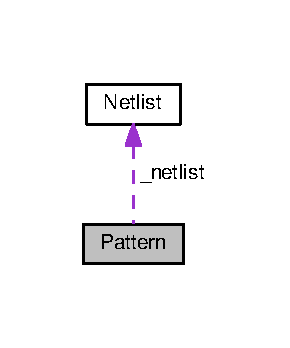
\includegraphics[width=139pt]{classPattern__coll__graph}
\end{center}
\end{figure}
\subsection*{Public Member Functions}
\begin{DoxyCompactItemize}
\item 
\hyperlink{classPattern_a11345fc22f0ff9a01cff037c5a3e5115}{Pattern} (const \hyperlink{classNetlist}{Netlist} \&netlist)
\begin{DoxyCompactList}\small\item\em Constructor. \end{DoxyCompactList}\item 
\hyperlink{type_8h_af19eddb079bfea723256710b029c38e8}{Mos\+Pattern} \hyperlink{classPattern_a1214e024706aff22e44bb4f4266d8e97}{pattern} (\hyperlink{type_8h_a581e8093e28e7362f2b6937296190676}{Index\+Type} mos\+Id1, \hyperlink{type_8h_a581e8093e28e7362f2b6937296190676}{Index\+Type} mos\+Id2) const
\begin{DoxyCompactList}\small\item\em Return pattern for pair of mosfets. \end{DoxyCompactList}\end{DoxyCompactItemize}
\subsection*{Private Member Functions}
\begin{DoxyCompactItemize}
\item 
bool \hyperlink{classPattern_ab7112a78b0ed0c7638f1af9efdf80955}{matched\+Type} (\hyperlink{type_8h_a581e8093e28e7362f2b6937296190676}{Index\+Type} mos\+Id1, \hyperlink{type_8h_a581e8093e28e7362f2b6937296190676}{Index\+Type} mos\+Id2) const
\begin{DoxyCompactList}\small\item\em Return true if \hyperlink{classInst}{Inst} pair have same Inst\+Type. \end{DoxyCompactList}\item 
bool \hyperlink{classPattern_ae25db8902e007a9ab055e64f3347d65d}{matched\+Size} (\hyperlink{type_8h_a581e8093e28e7362f2b6937296190676}{Index\+Type} mos\+Id1, \hyperlink{type_8h_a581e8093e28e7362f2b6937296190676}{Index\+Type} mos\+Id2) const
\begin{DoxyCompactList}\small\item\em Return true if \hyperlink{classInst}{Inst} pair have same size attributes. \end{DoxyCompactList}\item 
bool \hyperlink{classPattern_a8e30aad375e98bbcdeab764705e68045}{diff\+Pair\+Input} (\hyperlink{type_8h_a581e8093e28e7362f2b6937296190676}{Index\+Type} mos\+Id1, \hyperlink{type_8h_a581e8093e28e7362f2b6937296190676}{Index\+Type} mos\+Id2) const
\begin{DoxyCompactList}\small\item\em Return true if fits \hyperlink{type_8h_af19eddb079bfea723256710b029c38e8ad45b64a7d6b85dde1b52dd5a18863933}{Mos\+Pattern\+::\+D\+I\+F\+F\+\_\+\+S\+O\+U\+R\+CE}. \end{DoxyCompactList}\item 
bool \hyperlink{classPattern_ad59ebd9a536a170735daf63126d71dea}{diff\+Pair\+Cascode} (\hyperlink{type_8h_a581e8093e28e7362f2b6937296190676}{Index\+Type} mos\+Id1, \hyperlink{type_8h_a581e8093e28e7362f2b6937296190676}{Index\+Type} mos\+Id2) const
\begin{DoxyCompactList}\small\item\em Return true if fits \hyperlink{type_8h_af19eddb079bfea723256710b029c38e8a1b7b3de4c92d42d8311e04be030655af}{Mos\+Pattern\+::\+D\+I\+F\+F\+\_\+\+C\+A\+S\+C\+O\+DE}. \end{DoxyCompactList}\item 
bool \hyperlink{classPattern_ab1334774aab3ce88b1d2d799e31f3bd9}{valid\+Pair\+Cascode} (\hyperlink{type_8h_a581e8093e28e7362f2b6937296190676}{Index\+Type} mos\+Id1, \hyperlink{type_8h_a581e8093e28e7362f2b6937296190676}{Index\+Type} mos\+Id2) const
\begin{DoxyCompactList}\small\item\em Return true if fits \hyperlink{type_8h_af19eddb079bfea723256710b029c38e8aac50017227efb09ec529757764e5187c}{Mos\+Pattern\+::\+C\+A\+S\+C\+O\+DE}. \end{DoxyCompactList}\item 
bool \hyperlink{classPattern_acae638957d000c1a163f949c369d5ef4}{valid\+Pair\+Load} (\hyperlink{type_8h_a581e8093e28e7362f2b6937296190676}{Index\+Type} mos\+Id1, \hyperlink{type_8h_a581e8093e28e7362f2b6937296190676}{Index\+Type} mos\+Id2) const
\begin{DoxyCompactList}\small\item\em Return true if fits \hyperlink{type_8h_af19eddb079bfea723256710b029c38e8a615d2885ef7576cedd9aafbb2578f028}{Mos\+Pattern\+::\+L\+O\+AD}. \end{DoxyCompactList}\item 
bool \hyperlink{classPattern_a371cef1fc7d0c4d5b291d80dc5c4b777}{cross\+Pair\+Cascode} (\hyperlink{type_8h_a581e8093e28e7362f2b6937296190676}{Index\+Type} mos\+Id1, \hyperlink{type_8h_a581e8093e28e7362f2b6937296190676}{Index\+Type} mos\+Id2) const
\begin{DoxyCompactList}\small\item\em Return true if fits \hyperlink{type_8h_af19eddb079bfea723256710b029c38e8adb952aa3809767bf108688a754ebbf2c}{Mos\+Pattern\+::\+C\+R\+O\+S\+S\+\_\+\+C\+A\+S\+C\+O\+DE}. \end{DoxyCompactList}\item 
bool \hyperlink{classPattern_afe6e5456a639417112340f5f9d164b32}{cross\+Pair\+Load} (\hyperlink{type_8h_a581e8093e28e7362f2b6937296190676}{Index\+Type} mos\+Id1, \hyperlink{type_8h_a581e8093e28e7362f2b6937296190676}{Index\+Type} mos\+Id2) const
\begin{DoxyCompactList}\small\item\em Return true if fits \hyperlink{type_8h_af19eddb079bfea723256710b029c38e8a19ddbfeab78ac1a4bbe1a186828c5d8d}{Mos\+Pattern\+::\+C\+R\+O\+S\+S\+\_\+\+L\+O\+AD}. \end{DoxyCompactList}\item 
bool \hyperlink{classPattern_acbeabf067e49ed1ea743d647f541a3f4}{cap\+Mos} (\hyperlink{type_8h_a581e8093e28e7362f2b6937296190676}{Index\+Type} mos\+Id1, \hyperlink{type_8h_a581e8093e28e7362f2b6937296190676}{Index\+Type} mos\+Id2) const
\begin{DoxyCompactList}\small\item\em Return true if Mosfets are forming matched cap. \end{DoxyCompactList}\end{DoxyCompactItemize}
\subsection*{Private Attributes}
\begin{DoxyCompactItemize}
\item 
const \hyperlink{classNetlist}{Netlist} \& \hyperlink{classPattern_a71ec4e16ee6088587cece41cb7b027a3}{\+\_\+netlist}
\end{DoxyCompactItemize}


\subsection{Detailed Description}
\hyperlink{classPattern}{Pattern} class. 

\subsection{Constructor \& Destructor Documentation}
\mbox{\Hypertarget{classPattern_a11345fc22f0ff9a01cff037c5a3e5115}\label{classPattern_a11345fc22f0ff9a01cff037c5a3e5115}} 
\index{Pattern@{Pattern}!Pattern@{Pattern}}
\index{Pattern@{Pattern}!Pattern@{Pattern}}
\subsubsection{\texorpdfstring{Pattern()}{Pattern()}}
{\footnotesize\ttfamily Pattern\+::\+Pattern (\begin{DoxyParamCaption}\item[{const \hyperlink{classNetlist}{Netlist} \&}]{netlist }\end{DoxyParamCaption})\hspace{0.3cm}{\ttfamily [inline]}, {\ttfamily [explicit]}}



Constructor. 


\begin{DoxyParams}{Parameters}
{\em netlist} & \hyperlink{classNetlist}{Netlist} for pattern search. \\
\hline
\end{DoxyParams}


\subsection{Member Function Documentation}
\mbox{\Hypertarget{classPattern_acbeabf067e49ed1ea743d647f541a3f4}\label{classPattern_acbeabf067e49ed1ea743d647f541a3f4}} 
\index{Pattern@{Pattern}!cap\+Mos@{cap\+Mos}}
\index{cap\+Mos@{cap\+Mos}!Pattern@{Pattern}}
\subsubsection{\texorpdfstring{cap\+Mos()}{capMos()}}
{\footnotesize\ttfamily bool Pattern\+::cap\+Mos (\begin{DoxyParamCaption}\item[{\hyperlink{type_8h_a581e8093e28e7362f2b6937296190676}{Index\+Type}}]{mos\+Id1,  }\item[{\hyperlink{type_8h_a581e8093e28e7362f2b6937296190676}{Index\+Type}}]{mos\+Id2 }\end{DoxyParamCaption}) const\hspace{0.3cm}{\ttfamily [private]}}



Return true if Mosfets are forming matched cap. 

\mbox{\Hypertarget{classPattern_a371cef1fc7d0c4d5b291d80dc5c4b777}\label{classPattern_a371cef1fc7d0c4d5b291d80dc5c4b777}} 
\index{Pattern@{Pattern}!cross\+Pair\+Cascode@{cross\+Pair\+Cascode}}
\index{cross\+Pair\+Cascode@{cross\+Pair\+Cascode}!Pattern@{Pattern}}
\subsubsection{\texorpdfstring{cross\+Pair\+Cascode()}{crossPairCascode()}}
{\footnotesize\ttfamily bool Pattern\+::cross\+Pair\+Cascode (\begin{DoxyParamCaption}\item[{\hyperlink{type_8h_a581e8093e28e7362f2b6937296190676}{Index\+Type}}]{mos\+Id1,  }\item[{\hyperlink{type_8h_a581e8093e28e7362f2b6937296190676}{Index\+Type}}]{mos\+Id2 }\end{DoxyParamCaption}) const\hspace{0.3cm}{\ttfamily [private]}}



Return true if fits \hyperlink{type_8h_af19eddb079bfea723256710b029c38e8adb952aa3809767bf108688a754ebbf2c}{Mos\+Pattern\+::\+C\+R\+O\+S\+S\+\_\+\+C\+A\+S\+C\+O\+DE}. 

\mbox{\Hypertarget{classPattern_afe6e5456a639417112340f5f9d164b32}\label{classPattern_afe6e5456a639417112340f5f9d164b32}} 
\index{Pattern@{Pattern}!cross\+Pair\+Load@{cross\+Pair\+Load}}
\index{cross\+Pair\+Load@{cross\+Pair\+Load}!Pattern@{Pattern}}
\subsubsection{\texorpdfstring{cross\+Pair\+Load()}{crossPairLoad()}}
{\footnotesize\ttfamily bool Pattern\+::cross\+Pair\+Load (\begin{DoxyParamCaption}\item[{\hyperlink{type_8h_a581e8093e28e7362f2b6937296190676}{Index\+Type}}]{mos\+Id1,  }\item[{\hyperlink{type_8h_a581e8093e28e7362f2b6937296190676}{Index\+Type}}]{mos\+Id2 }\end{DoxyParamCaption}) const\hspace{0.3cm}{\ttfamily [private]}}



Return true if fits \hyperlink{type_8h_af19eddb079bfea723256710b029c38e8a19ddbfeab78ac1a4bbe1a186828c5d8d}{Mos\+Pattern\+::\+C\+R\+O\+S\+S\+\_\+\+L\+O\+AD}. 

\mbox{\Hypertarget{classPattern_ad59ebd9a536a170735daf63126d71dea}\label{classPattern_ad59ebd9a536a170735daf63126d71dea}} 
\index{Pattern@{Pattern}!diff\+Pair\+Cascode@{diff\+Pair\+Cascode}}
\index{diff\+Pair\+Cascode@{diff\+Pair\+Cascode}!Pattern@{Pattern}}
\subsubsection{\texorpdfstring{diff\+Pair\+Cascode()}{diffPairCascode()}}
{\footnotesize\ttfamily bool Pattern\+::diff\+Pair\+Cascode (\begin{DoxyParamCaption}\item[{\hyperlink{type_8h_a581e8093e28e7362f2b6937296190676}{Index\+Type}}]{mos\+Id1,  }\item[{\hyperlink{type_8h_a581e8093e28e7362f2b6937296190676}{Index\+Type}}]{mos\+Id2 }\end{DoxyParamCaption}) const\hspace{0.3cm}{\ttfamily [private]}}



Return true if fits \hyperlink{type_8h_af19eddb079bfea723256710b029c38e8a1b7b3de4c92d42d8311e04be030655af}{Mos\+Pattern\+::\+D\+I\+F\+F\+\_\+\+C\+A\+S\+C\+O\+DE}. 

\mbox{\Hypertarget{classPattern_a8e30aad375e98bbcdeab764705e68045}\label{classPattern_a8e30aad375e98bbcdeab764705e68045}} 
\index{Pattern@{Pattern}!diff\+Pair\+Input@{diff\+Pair\+Input}}
\index{diff\+Pair\+Input@{diff\+Pair\+Input}!Pattern@{Pattern}}
\subsubsection{\texorpdfstring{diff\+Pair\+Input()}{diffPairInput()}}
{\footnotesize\ttfamily bool Pattern\+::diff\+Pair\+Input (\begin{DoxyParamCaption}\item[{\hyperlink{type_8h_a581e8093e28e7362f2b6937296190676}{Index\+Type}}]{mos\+Id1,  }\item[{\hyperlink{type_8h_a581e8093e28e7362f2b6937296190676}{Index\+Type}}]{mos\+Id2 }\end{DoxyParamCaption}) const\hspace{0.3cm}{\ttfamily [private]}}



Return true if fits \hyperlink{type_8h_af19eddb079bfea723256710b029c38e8ad45b64a7d6b85dde1b52dd5a18863933}{Mos\+Pattern\+::\+D\+I\+F\+F\+\_\+\+S\+O\+U\+R\+CE}. 

\mbox{\Hypertarget{classPattern_ae25db8902e007a9ab055e64f3347d65d}\label{classPattern_ae25db8902e007a9ab055e64f3347d65d}} 
\index{Pattern@{Pattern}!matched\+Size@{matched\+Size}}
\index{matched\+Size@{matched\+Size}!Pattern@{Pattern}}
\subsubsection{\texorpdfstring{matched\+Size()}{matchedSize()}}
{\footnotesize\ttfamily bool Pattern\+::matched\+Size (\begin{DoxyParamCaption}\item[{\hyperlink{type_8h_a581e8093e28e7362f2b6937296190676}{Index\+Type}}]{mos\+Id1,  }\item[{\hyperlink{type_8h_a581e8093e28e7362f2b6937296190676}{Index\+Type}}]{mos\+Id2 }\end{DoxyParamCaption}) const\hspace{0.3cm}{\ttfamily [private]}}



Return true if \hyperlink{classInst}{Inst} pair have same size attributes. 

\mbox{\Hypertarget{classPattern_ab7112a78b0ed0c7638f1af9efdf80955}\label{classPattern_ab7112a78b0ed0c7638f1af9efdf80955}} 
\index{Pattern@{Pattern}!matched\+Type@{matched\+Type}}
\index{matched\+Type@{matched\+Type}!Pattern@{Pattern}}
\subsubsection{\texorpdfstring{matched\+Type()}{matchedType()}}
{\footnotesize\ttfamily \hyperlink{namespace_8h_ae48726a24dab2034454cf6d79e531eb8}{P\+R\+O\+J\+E\+C\+T\+\_\+\+N\+A\+M\+E\+S\+P\+A\+C\+E\+\_\+\+B\+E\+G\+IN} bool Pattern\+::matched\+Type (\begin{DoxyParamCaption}\item[{\hyperlink{type_8h_a581e8093e28e7362f2b6937296190676}{Index\+Type}}]{mos\+Id1,  }\item[{\hyperlink{type_8h_a581e8093e28e7362f2b6937296190676}{Index\+Type}}]{mos\+Id2 }\end{DoxyParamCaption}) const\hspace{0.3cm}{\ttfamily [private]}}



Return true if \hyperlink{classInst}{Inst} pair have same Inst\+Type. 

\mbox{\Hypertarget{classPattern_a1214e024706aff22e44bb4f4266d8e97}\label{classPattern_a1214e024706aff22e44bb4f4266d8e97}} 
\index{Pattern@{Pattern}!pattern@{pattern}}
\index{pattern@{pattern}!Pattern@{Pattern}}
\subsubsection{\texorpdfstring{pattern()}{pattern()}}
{\footnotesize\ttfamily \hyperlink{type_8h_af19eddb079bfea723256710b029c38e8}{Mos\+Pattern} Pattern\+::pattern (\begin{DoxyParamCaption}\item[{\hyperlink{type_8h_a581e8093e28e7362f2b6937296190676}{Index\+Type}}]{mos\+Id1,  }\item[{\hyperlink{type_8h_a581e8093e28e7362f2b6937296190676}{Index\+Type}}]{mos\+Id2 }\end{DoxyParamCaption}) const}



Return pattern for pair of mosfets. 

Valid patterns have same Inst\+Type. Currently they also have same size attribute.

T\+O\+DO Add ratio pair detection in future. \begin{DoxySeeAlso}{See also}
\hyperlink{type_8h_af19eddb079bfea723256710b029c38e8}{Mos\+Pattern}. 
\end{DoxySeeAlso}

\begin{DoxyParams}{Parameters}
{\em mos\+Id1} & Id for mosfet. \\
\hline
{\em mos\+Id2} & Id for mosfet. \\
\hline
\end{DoxyParams}
\mbox{\Hypertarget{classPattern_ab1334774aab3ce88b1d2d799e31f3bd9}\label{classPattern_ab1334774aab3ce88b1d2d799e31f3bd9}} 
\index{Pattern@{Pattern}!valid\+Pair\+Cascode@{valid\+Pair\+Cascode}}
\index{valid\+Pair\+Cascode@{valid\+Pair\+Cascode}!Pattern@{Pattern}}
\subsubsection{\texorpdfstring{valid\+Pair\+Cascode()}{validPairCascode()}}
{\footnotesize\ttfamily bool Pattern\+::valid\+Pair\+Cascode (\begin{DoxyParamCaption}\item[{\hyperlink{type_8h_a581e8093e28e7362f2b6937296190676}{Index\+Type}}]{mos\+Id1,  }\item[{\hyperlink{type_8h_a581e8093e28e7362f2b6937296190676}{Index\+Type}}]{mos\+Id2 }\end{DoxyParamCaption}) const\hspace{0.3cm}{\ttfamily [private]}}



Return true if fits \hyperlink{type_8h_af19eddb079bfea723256710b029c38e8aac50017227efb09ec529757764e5187c}{Mos\+Pattern\+::\+C\+A\+S\+C\+O\+DE}. 

\mbox{\Hypertarget{classPattern_acae638957d000c1a163f949c369d5ef4}\label{classPattern_acae638957d000c1a163f949c369d5ef4}} 
\index{Pattern@{Pattern}!valid\+Pair\+Load@{valid\+Pair\+Load}}
\index{valid\+Pair\+Load@{valid\+Pair\+Load}!Pattern@{Pattern}}
\subsubsection{\texorpdfstring{valid\+Pair\+Load()}{validPairLoad()}}
{\footnotesize\ttfamily bool Pattern\+::valid\+Pair\+Load (\begin{DoxyParamCaption}\item[{\hyperlink{type_8h_a581e8093e28e7362f2b6937296190676}{Index\+Type}}]{mos\+Id1,  }\item[{\hyperlink{type_8h_a581e8093e28e7362f2b6937296190676}{Index\+Type}}]{mos\+Id2 }\end{DoxyParamCaption}) const\hspace{0.3cm}{\ttfamily [private]}}



Return true if fits \hyperlink{type_8h_af19eddb079bfea723256710b029c38e8a615d2885ef7576cedd9aafbb2578f028}{Mos\+Pattern\+::\+L\+O\+AD}. 



\subsection{Member Data Documentation}
\mbox{\Hypertarget{classPattern_a71ec4e16ee6088587cece41cb7b027a3}\label{classPattern_a71ec4e16ee6088587cece41cb7b027a3}} 
\index{Pattern@{Pattern}!\+\_\+netlist@{\+\_\+netlist}}
\index{\+\_\+netlist@{\+\_\+netlist}!Pattern@{Pattern}}
\subsubsection{\texorpdfstring{\+\_\+netlist}{\_netlist}}
{\footnotesize\ttfamily const \hyperlink{classNetlist}{Netlist}\& Pattern\+::\+\_\+netlist\hspace{0.3cm}{\ttfamily [private]}}



The documentation for this class was generated from the following files\+:\begin{DoxyCompactItemize}
\item 
src/sym\+\_\+detect/\hyperlink{Pattern_8h}{Pattern.\+h}\item 
src/sym\+\_\+detect/\hyperlink{Pattern_8cpp}{Pattern.\+cpp}\end{DoxyCompactItemize}

\hypertarget{classPin}{}\section{Pin Class Reference}
\label{classPin}\index{Pin@{Pin}}


\hyperlink{classPin}{Pin} class.  




{\ttfamily \#include $<$Pin.\+h$>$}

\subsection*{Public Member Functions}
\begin{DoxyCompactItemize}
\item 
\hyperlink{classPin_a6fbd67b1c9ed59f0af668f675bbc561f}{Pin} ()=default
\item 
\hyperlink{classPin_aa8987e1d2ee361faa8929c98953a03f2}{Pin} (\hyperlink{type_8h_a581e8093e28e7362f2b6937296190676}{Index\+Type} \hyperlink{classPin_a36da1568fe78213394b67a5a470ffb00}{id}, \hyperlink{type_8h_a581e8093e28e7362f2b6937296190676}{Index\+Type} \hyperlink{classPin_a8ddc3b130a28cbc1781b155dea8c333e}{inst\+Id}, \hyperlink{type_8h_a581e8093e28e7362f2b6937296190676}{Index\+Type} \hyperlink{classPin_a5bcc2c816d52b915690738820c4042b3}{net\+Id}, \hyperlink{type_8h_afaab50027002ecbb6c8ac27e727d1bb4}{Pin\+Type} \hyperlink{classPin_a788397e41a9a4fa196b36f8076eb6d6c}{type})
\begin{DoxyCompactList}\small\item\em Constructor for \hyperlink{classPin}{Pin}. \end{DoxyCompactList}\item 
\hyperlink{type_8h_a581e8093e28e7362f2b6937296190676}{Index\+Type} \hyperlink{classPin_a36da1568fe78213394b67a5a470ffb00}{id} () const
\item 
\hyperlink{type_8h_a581e8093e28e7362f2b6937296190676}{Index\+Type} \hyperlink{classPin_a8ddc3b130a28cbc1781b155dea8c333e}{inst\+Id} () const
\item 
\hyperlink{type_8h_a581e8093e28e7362f2b6937296190676}{Index\+Type} \hyperlink{classPin_a5bcc2c816d52b915690738820c4042b3}{net\+Id} () const
\item 
\hyperlink{type_8h_afaab50027002ecbb6c8ac27e727d1bb4}{Pin\+Type} \hyperlink{classPin_a788397e41a9a4fa196b36f8076eb6d6c}{type} () const
\begin{DoxyCompactList}\small\item\em Return type of \hyperlink{classPin}{Pin}. \end{DoxyCompactList}\end{DoxyCompactItemize}
\subsection*{Static Public Member Functions}
\begin{DoxyCompactItemize}
\item 
static \hyperlink{type_8h_afaab50027002ecbb6c8ac27e727d1bb4}{Pin\+Type} \hyperlink{classPin_a86313ccf5cf94894c0d6cece183cb25d}{next\+Pin\+Type} (\hyperlink{type_8h_afaab50027002ecbb6c8ac27e727d1bb4}{Pin\+Type} \hyperlink{classPin_a788397e41a9a4fa196b36f8076eb6d6c}{type})
\begin{DoxyCompactList}\small\item\em Return the next search Pin\+Type for D\+FS. \end{DoxyCompactList}\end{DoxyCompactItemize}
\subsection*{Private Attributes}
\begin{DoxyCompactItemize}
\item 
\hyperlink{type_8h_a581e8093e28e7362f2b6937296190676}{Index\+Type} \hyperlink{classPin_ad40a8453e8fa16e12e17f661bfc36f69}{\+\_\+id}
\item 
\hyperlink{type_8h_a581e8093e28e7362f2b6937296190676}{Index\+Type} \hyperlink{classPin_aa9bd5211cedd081a572476545f5bf498}{\+\_\+inst\+Id}
\item 
\hyperlink{type_8h_a581e8093e28e7362f2b6937296190676}{Index\+Type} \hyperlink{classPin_a703ff6aea39f28b40e7d5d4dfb708a67}{\+\_\+net\+Id}
\item 
\hyperlink{type_8h_afaab50027002ecbb6c8ac27e727d1bb4}{Pin\+Type} \hyperlink{classPin_a0a660d777203aca04685f4cdf6623f72}{\+\_\+type}
\end{DoxyCompactItemize}


\subsection{Detailed Description}
\hyperlink{classPin}{Pin} class. 

\subsection{Constructor \& Destructor Documentation}
\mbox{\Hypertarget{classPin_a6fbd67b1c9ed59f0af668f675bbc561f}\label{classPin_a6fbd67b1c9ed59f0af668f675bbc561f}} 
\index{Pin@{Pin}!Pin@{Pin}}
\index{Pin@{Pin}!Pin@{Pin}}
\subsubsection{\texorpdfstring{Pin()}{Pin()}\hspace{0.1cm}{\footnotesize\ttfamily [1/2]}}
{\footnotesize\ttfamily Pin\+::\+Pin (\begin{DoxyParamCaption}{ }\end{DoxyParamCaption})\hspace{0.3cm}{\ttfamily [explicit]}, {\ttfamily [default]}}

Default Constructor. \mbox{\Hypertarget{classPin_aa8987e1d2ee361faa8929c98953a03f2}\label{classPin_aa8987e1d2ee361faa8929c98953a03f2}} 
\index{Pin@{Pin}!Pin@{Pin}}
\index{Pin@{Pin}!Pin@{Pin}}
\subsubsection{\texorpdfstring{Pin()}{Pin()}\hspace{0.1cm}{\footnotesize\ttfamily [2/2]}}
{\footnotesize\ttfamily Pin\+::\+Pin (\begin{DoxyParamCaption}\item[{\hyperlink{type_8h_a581e8093e28e7362f2b6937296190676}{Index\+Type}}]{id,  }\item[{\hyperlink{type_8h_a581e8093e28e7362f2b6937296190676}{Index\+Type}}]{inst\+Id,  }\item[{\hyperlink{type_8h_a581e8093e28e7362f2b6937296190676}{Index\+Type}}]{net\+Id,  }\item[{\hyperlink{type_8h_afaab50027002ecbb6c8ac27e727d1bb4}{Pin\+Type}}]{type }\end{DoxyParamCaption})\hspace{0.3cm}{\ttfamily [inline]}, {\ttfamily [explicit]}}



Constructor for \hyperlink{classPin}{Pin}. 


\begin{DoxyParams}{Parameters}
{\em id} & Id of \hyperlink{classPin}{Pin}. \\
\hline
{\em inst\+Id} & Id of connected \hyperlink{classInst}{Inst}. \\
\hline
{\em net\+Id} & Id of connected \hyperlink{classNet}{Net}. \\
\hline
{\em type} & Type of \hyperlink{classPin}{Pin}. \\
\hline
\end{DoxyParams}


\subsection{Member Function Documentation}
\mbox{\Hypertarget{classPin_a36da1568fe78213394b67a5a470ffb00}\label{classPin_a36da1568fe78213394b67a5a470ffb00}} 
\index{Pin@{Pin}!id@{id}}
\index{id@{id}!Pin@{Pin}}
\subsubsection{\texorpdfstring{id()}{id()}}
{\footnotesize\ttfamily \hyperlink{type_8h_a581e8093e28e7362f2b6937296190676}{Index\+Type} Pin\+::id (\begin{DoxyParamCaption}{ }\end{DoxyParamCaption}) const\hspace{0.3cm}{\ttfamily [inline]}}

Return id of \hyperlink{classPin}{Pin}. \mbox{\Hypertarget{classPin_a8ddc3b130a28cbc1781b155dea8c333e}\label{classPin_a8ddc3b130a28cbc1781b155dea8c333e}} 
\index{Pin@{Pin}!inst\+Id@{inst\+Id}}
\index{inst\+Id@{inst\+Id}!Pin@{Pin}}
\subsubsection{\texorpdfstring{inst\+Id()}{instId()}}
{\footnotesize\ttfamily \hyperlink{type_8h_a581e8093e28e7362f2b6937296190676}{Index\+Type} Pin\+::inst\+Id (\begin{DoxyParamCaption}{ }\end{DoxyParamCaption}) const\hspace{0.3cm}{\ttfamily [inline]}}

Return id of connected \hyperlink{classInst}{Inst}. \mbox{\Hypertarget{classPin_a5bcc2c816d52b915690738820c4042b3}\label{classPin_a5bcc2c816d52b915690738820c4042b3}} 
\index{Pin@{Pin}!net\+Id@{net\+Id}}
\index{net\+Id@{net\+Id}!Pin@{Pin}}
\subsubsection{\texorpdfstring{net\+Id()}{netId()}}
{\footnotesize\ttfamily \hyperlink{type_8h_a581e8093e28e7362f2b6937296190676}{Index\+Type} Pin\+::net\+Id (\begin{DoxyParamCaption}{ }\end{DoxyParamCaption}) const\hspace{0.3cm}{\ttfamily [inline]}}

Return id of connected \hyperlink{classNet}{Net}. \mbox{\Hypertarget{classPin_a86313ccf5cf94894c0d6cece183cb25d}\label{classPin_a86313ccf5cf94894c0d6cece183cb25d}} 
\index{Pin@{Pin}!next\+Pin\+Type@{next\+Pin\+Type}}
\index{next\+Pin\+Type@{next\+Pin\+Type}!Pin@{Pin}}
\subsubsection{\texorpdfstring{next\+Pin\+Type()}{nextPinType()}}
{\footnotesize\ttfamily \hyperlink{namespace_8h_ae48726a24dab2034454cf6d79e531eb8}{P\+R\+O\+J\+E\+C\+T\+\_\+\+N\+A\+M\+E\+S\+P\+A\+C\+E\+\_\+\+B\+E\+G\+IN} \hyperlink{type_8h_afaab50027002ecbb6c8ac27e727d1bb4}{Pin\+Type} Pin\+::next\+Pin\+Type (\begin{DoxyParamCaption}\item[{\hyperlink{type_8h_afaab50027002ecbb6c8ac27e727d1bb4}{Pin\+Type}}]{type }\end{DoxyParamCaption})\hspace{0.3cm}{\ttfamily [static]}}



Return the next search Pin\+Type for D\+FS. 


\begin{DoxyParams}{Parameters}
{\em type} & Querry the next search Pin\+Type. \\
\hline
\end{DoxyParams}
\begin{DoxySeeAlso}{See also}
\hyperlink{type_8h_afaab50027002ecbb6c8ac27e727d1bb4}{Pin\+Type}
\end{DoxySeeAlso}
The D\+FS search for symmetry relys on \hyperlink{classPin_a86313ccf5cf94894c0d6cece183cb25d}{Pin\+::next\+Pin\+Type} to define the search path direction. For example, if a Mosfet was reached through a source then the D\+FS algorithm would search for connected \hyperlink{classInst}{Inst} of the drain. Currently supported search paths\+: \tabulinesep=1mm
\begin{longtabu} spread 0pt [c]{*{2}{|X[-1]}|}
\hline
\rowcolor{\tableheadbgcolor}\textbf{ Input Pin\+Type }&\textbf{ next\+Pin\+Type  }\\\cline{1-2}
\endfirsthead
\hline
\endfoot
\hline
\rowcolor{\tableheadbgcolor}\textbf{ Input Pin\+Type }&\textbf{ next\+Pin\+Type  }\\\cline{1-2}
\endhead
S\+O\+U\+R\+CE &D\+R\+A\+IN \\\cline{1-2}
D\+R\+A\+IN &S\+O\+U\+R\+CE \\\cline{1-2}
T\+H\+IS &T\+H\+AT \\\cline{1-2}
T\+H\+AT &T\+H\+IS \\\cline{1-2}
\end{longtabu}
\mbox{\Hypertarget{classPin_a788397e41a9a4fa196b36f8076eb6d6c}\label{classPin_a788397e41a9a4fa196b36f8076eb6d6c}} 
\index{Pin@{Pin}!type@{type}}
\index{type@{type}!Pin@{Pin}}
\subsubsection{\texorpdfstring{type()}{type()}}
{\footnotesize\ttfamily \hyperlink{type_8h_afaab50027002ecbb6c8ac27e727d1bb4}{Pin\+Type} Pin\+::type (\begin{DoxyParamCaption}{ }\end{DoxyParamCaption}) const\hspace{0.3cm}{\ttfamily [inline]}}



Return type of \hyperlink{classPin}{Pin}. 

\begin{DoxySeeAlso}{See also}
\hyperlink{type_8h_afaab50027002ecbb6c8ac27e727d1bb4}{Pin\+Type} 
\end{DoxySeeAlso}


\subsection{Member Data Documentation}
\mbox{\Hypertarget{classPin_ad40a8453e8fa16e12e17f661bfc36f69}\label{classPin_ad40a8453e8fa16e12e17f661bfc36f69}} 
\index{Pin@{Pin}!\+\_\+id@{\+\_\+id}}
\index{\+\_\+id@{\+\_\+id}!Pin@{Pin}}
\subsubsection{\texorpdfstring{\+\_\+id}{\_id}}
{\footnotesize\ttfamily \hyperlink{type_8h_a581e8093e28e7362f2b6937296190676}{Index\+Type} Pin\+::\+\_\+id\hspace{0.3cm}{\ttfamily [private]}}

\mbox{\Hypertarget{classPin_aa9bd5211cedd081a572476545f5bf498}\label{classPin_aa9bd5211cedd081a572476545f5bf498}} 
\index{Pin@{Pin}!\+\_\+inst\+Id@{\+\_\+inst\+Id}}
\index{\+\_\+inst\+Id@{\+\_\+inst\+Id}!Pin@{Pin}}
\subsubsection{\texorpdfstring{\+\_\+inst\+Id}{\_instId}}
{\footnotesize\ttfamily \hyperlink{type_8h_a581e8093e28e7362f2b6937296190676}{Index\+Type} Pin\+::\+\_\+inst\+Id\hspace{0.3cm}{\ttfamily [private]}}

\mbox{\Hypertarget{classPin_a703ff6aea39f28b40e7d5d4dfb708a67}\label{classPin_a703ff6aea39f28b40e7d5d4dfb708a67}} 
\index{Pin@{Pin}!\+\_\+net\+Id@{\+\_\+net\+Id}}
\index{\+\_\+net\+Id@{\+\_\+net\+Id}!Pin@{Pin}}
\subsubsection{\texorpdfstring{\+\_\+net\+Id}{\_netId}}
{\footnotesize\ttfamily \hyperlink{type_8h_a581e8093e28e7362f2b6937296190676}{Index\+Type} Pin\+::\+\_\+net\+Id\hspace{0.3cm}{\ttfamily [private]}}

\mbox{\Hypertarget{classPin_a0a660d777203aca04685f4cdf6623f72}\label{classPin_a0a660d777203aca04685f4cdf6623f72}} 
\index{Pin@{Pin}!\+\_\+type@{\+\_\+type}}
\index{\+\_\+type@{\+\_\+type}!Pin@{Pin}}
\subsubsection{\texorpdfstring{\+\_\+type}{\_type}}
{\footnotesize\ttfamily \hyperlink{type_8h_afaab50027002ecbb6c8ac27e727d1bb4}{Pin\+Type} Pin\+::\+\_\+type\hspace{0.3cm}{\ttfamily [private]}}



The documentation for this class was generated from the following files\+:\begin{DoxyCompactItemize}
\item 
src/db/\hyperlink{Pin_8h}{Pin.\+h}\item 
src/db/\hyperlink{Pin_8cpp}{Pin.\+cpp}\end{DoxyCompactItemize}

\hypertarget{classSymDetect}{}\section{Sym\+Detect Class Reference}
\label{classSymDetect}\index{Sym\+Detect@{Sym\+Detect}}


\hyperlink{classSymDetect}{Sym\+Detect} class.  




{\ttfamily \#include $<$Sym\+Detect.\+h$>$}



Collaboration diagram for Sym\+Detect\+:\nopagebreak
\begin{figure}[H]
\begin{center}
\leavevmode
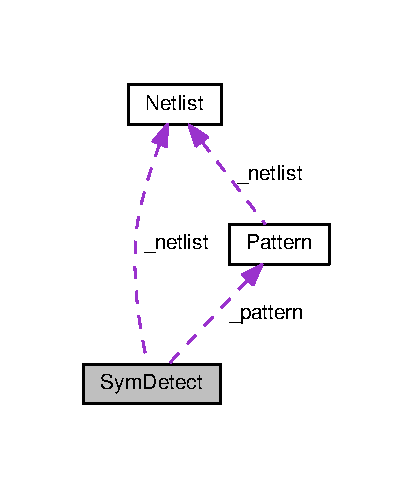
\includegraphics[width=198pt]{classSymDetect__coll__graph}
\end{center}
\end{figure}
\subsection*{Public Member Functions}
\begin{DoxyCompactItemize}
\item 
\hyperlink{classSymDetect_aaf0ca6563b2168db22cfd313ec773c23}{Sym\+Detect} (const \hyperlink{classNetlist}{Netlist} \&netlist)
\begin{DoxyCompactList}\small\item\em Constructor Only needs netlist as input. \hyperlink{classPattern}{Pattern} class inherently constructed. \end{DoxyCompactList}\item 
void \hyperlink{classSymDetect_a3e0354c4c11fe698377a4688c52fd533}{print} () const
\begin{DoxyCompactList}\small\item\em Print sym\+Group for netlist. \end{DoxyCompactList}\item 
void \hyperlink{classSymDetect_a12ab74214af31ed8fc5608e958e74786}{dump\+Sym} (const std\+::string file) const
\begin{DoxyCompactList}\small\item\em Dump symmetry constraint to file. \end{DoxyCompactList}\item 
void \hyperlink{classSymDetect_afe5e834e590ac2e055a17b6c951098d0}{dump\+Net} (const std\+::string file) const
\begin{DoxyCompactList}\small\item\em Dump symmetry net to file. \end{DoxyCompactList}\end{DoxyCompactItemize}
\subsection*{Private Member Functions}
\begin{DoxyCompactItemize}
\item 
\hyperlink{type_8h_af19eddb079bfea723256710b029c38e8}{Mos\+Pattern} \hyperlink{classSymDetect_aa832e51051f0ed9d3643c72b1d738684}{Mos\+Pair\+Ptrn} (\hyperlink{classMosPair}{Mos\+Pair} \&obj) const
\begin{DoxyCompactList}\small\item\em Return pattern of \hyperlink{classMosPair}{Mos\+Pair}. \end{DoxyCompactList}\item 
bool \hyperlink{classSymDetect_a58ba284bb8522714804a192b2720cae3}{exist\+Pair} (const std\+::vector$<$ \hyperlink{classMosPair}{Mos\+Pair} $>$ \&library, \hyperlink{type_8h_a581e8093e28e7362f2b6937296190676}{Index\+Type} inst\+Id1, \hyperlink{type_8h_a581e8093e28e7362f2b6937296190676}{Index\+Type} inst\+Id2) const
\begin{DoxyCompactList}\small\item\em Check if pair already reached. \end{DoxyCompactList}\item 
bool \hyperlink{classSymDetect_a72b24ce0ad3992c207f5023250dd1d5a}{exist\+Pair} (std\+::vector$<$ \hyperlink{classMosPair}{Mos\+Pair} $>$ \&library, \hyperlink{type_8h_a581e8093e28e7362f2b6937296190676}{Index\+Type} inst\+Id) const
\item 
bool \hyperlink{classSymDetect_a0e73f6d9d0b83b0c42c569fc42f8ecd2}{exist\+Net\+Pair} (std\+::vector$<$ \hyperlink{classNetPair}{Net\+Pair} $>$ \&library, \hyperlink{type_8h_a581e8093e28e7362f2b6937296190676}{Index\+Type} net\+Id1, \hyperlink{type_8h_a581e8093e28e7362f2b6937296190676}{Index\+Type} net\+Id2) const
\begin{DoxyCompactList}\small\item\em Check if already contains \hyperlink{classNetPair}{Net\+Pair} in library. \end{DoxyCompactList}\item 
bool \hyperlink{classSymDetect_a04b449b545fe7d175e4733b3f602c41c}{exist\+Net\+Pair} (std\+::vector$<$ \hyperlink{classNetPair}{Net\+Pair} $>$ \&library, \hyperlink{type_8h_a581e8093e28e7362f2b6937296190676}{Index\+Type} net\+Id) const
\begin{DoxyCompactList}\small\item\em Check if self symmetry \hyperlink{classNet}{Net} in library. \end{DoxyCompactList}\item 
bool \hyperlink{classSymDetect_ac46824a93f71489b6c9f1aec961a0f8d}{end\+Srch} (\hyperlink{classMosPair}{Mos\+Pair} \&obj) const
\begin{DoxyCompactList}\small\item\em Return true if end of search path. \end{DoxyCompactList}\item 
bool \hyperlink{classSymDetect_ad4636f69ae0cad2fc23be2472c59ff4c}{valid\+Srch\+Obj} (\hyperlink{type_8h_a581e8093e28e7362f2b6937296190676}{Index\+Type} inst\+Id1, \hyperlink{type_8h_a581e8093e28e7362f2b6937296190676}{Index\+Type} inst\+Id2, \hyperlink{type_8h_a581e8093e28e7362f2b6937296190676}{Index\+Type} srch\+Pin\+Id1, \hyperlink{type_8h_a581e8093e28e7362f2b6937296190676}{Index\+Type} srch\+Pin\+Id2) const
\begin{DoxyCompactList}\small\item\em Return true if a valid pair. \end{DoxyCompactList}\item 
bool \hyperlink{classSymDetect_a1153c5f98df1f6dde97ed3335367bb66}{valid\+Diff\+Pair} (\hyperlink{type_8h_a581e8093e28e7362f2b6937296190676}{Index\+Type} inst\+Id1, \hyperlink{type_8h_a581e8093e28e7362f2b6937296190676}{Index\+Type} inst\+Id2, \hyperlink{type_8h_a581e8093e28e7362f2b6937296190676}{Index\+Type} srch\+Pin\+Id1, \hyperlink{type_8h_a581e8093e28e7362f2b6937296190676}{Index\+Type} srch\+Pin\+Id2) const
\begin{DoxyCompactList}\small\item\em Return true if a valid D\+I\+F\+F\+\_\+\+S\+O\+U\+R\+CE gate connected. \end{DoxyCompactList}\item 
bool \hyperlink{classSymDetect_a455e5f585e60c484e2d093a44775faf5}{valid\+Net\+Pair} (\hyperlink{type_8h_a581e8093e28e7362f2b6937296190676}{Index\+Type} net\+Id1, \hyperlink{type_8h_a581e8093e28e7362f2b6937296190676}{Index\+Type} net\+Id2, std\+::vector$<$ \hyperlink{classNetPair}{Net\+Pair} $>$ \&net\+Pair) const
\begin{DoxyCompactList}\small\item\em Return true if a valid symmetry \hyperlink{classNetPair}{Net\+Pair}. \end{DoxyCompactList}\item 
bool \hyperlink{classSymDetect_a6672756986d958695756a1fa2c76577d}{check\+Net\+Sym} (\hyperlink{type_8h_a581e8093e28e7362f2b6937296190676}{Index\+Type} net\+Id1, \hyperlink{type_8h_a581e8093e28e7362f2b6937296190676}{Index\+Type} net\+Id2) const
\begin{DoxyCompactList}\small\item\em Check every pin of nets for symmetry. \end{DoxyCompactList}\item 
void \hyperlink{classSymDetect_a7f4cd1010a21da88d35abb89c6f33f00}{push\+Next\+Srch\+Obj} (std\+::vector$<$ \hyperlink{classMosPair}{Mos\+Pair} $>$ \&dfs\+Vst\+Pair, std\+::vector$<$ \hyperlink{classMosPair}{Mos\+Pair} $>$ \&dfs\+Stack, \hyperlink{classMosPair}{Mos\+Pair} \&curr\+Obj, std\+::vector$<$ \hyperlink{classMosPair}{Mos\+Pair} $>$ \&diff\+Pair\+Src) const
\begin{DoxyCompactList}\small\item\em Push next valid \hyperlink{classMosPair}{Mos\+Pair} to dfs\+Stack. \end{DoxyCompactList}\item 
bool \hyperlink{classSymDetect_a13ddc56c5e937097178352eb00d71cf3}{com\+Bias} (\hyperlink{classMosPair}{Mos\+Pair} \&curr\+Obj) const
\begin{DoxyCompactList}\small\item\em Return true if curr\+Obj have common gate connection. \end{DoxyCompactList}\item 
void \hyperlink{classSymDetect_a79b9b8042087a413df53daf4e5600728}{add\+Bias\+Sym} (std\+::vector$<$ \hyperlink{classMosPair}{Mos\+Pair} $>$ \&dfs\+Vst\+Pair, \hyperlink{classMosPair}{Mos\+Pair} \&curr\+Obj) const
\begin{DoxyCompactList}\small\item\em A special case where a symmetry pair is formed in the bias group. \end{DoxyCompactList}\item 
void \hyperlink{classSymDetect_aa6d2ec13048f8f7e18e659bf8ac31dee}{get\+Patrn\+Net\+Conn} (std\+::vector$<$ \hyperlink{classMosPair}{Mos\+Pair} $>$ \&diff\+Pair, \hyperlink{type_8h_a581e8093e28e7362f2b6937296190676}{Index\+Type} net\+Id, \hyperlink{type_8h_af19eddb079bfea723256710b029c38e8}{Mos\+Pattern} srch\+Patrn) const
\begin{DoxyCompactList}\small\item\em Get srch\+Patrn \hyperlink{classMosPair}{Mos\+Pair} connected to net\+Id. \end{DoxyCompactList}\item 
void \hyperlink{classSymDetect_af04b93dac7e090cef8e741d8d1812485}{get\+Diff\+Pair} (std\+::vector$<$ \hyperlink{classMosPair}{Mos\+Pair} $>$ \&diff\+Pair) const
\begin{DoxyCompactList}\small\item\em Get valid D\+FS source of netlist. \end{DoxyCompactList}\item 
void \hyperlink{classSymDetect_acd33a2c834493240fc4e8840819d676c}{dfs\+Diff\+Pair} (std\+::vector$<$ \hyperlink{classMosPair}{Mos\+Pair} $>$ \&dfs\+Vst\+Pair, \hyperlink{classMosPair}{Mos\+Pair} \&diff\+Pair, std\+::vector$<$ \hyperlink{classMosPair}{Mos\+Pair} $>$ \&diff\+Pair\+Srch) const
\begin{DoxyCompactList}\small\item\em D\+FS search with given source. Visited \hyperlink{classMosPair}{Mos\+Pair} are stored. \end{DoxyCompactList}\item 
void \hyperlink{classSymDetect_ae6a1ba27f6768f215cba0623b6e2ce08}{in\+Vld\+Diff\+Pair\+Srch} (std\+::vector$<$ \hyperlink{classMosPair}{Mos\+Pair} $>$ \&diff\+Pair\+Srch, \hyperlink{classMosPair}{Mos\+Pair} \&curr\+Pair) const
\begin{DoxyCompactList}\small\item\em Invalidate visited pairs from sources. \end{DoxyCompactList}\item 
void \hyperlink{classSymDetect_a48c23173bf5e56c3aa11ac306715cba2}{get\+Vld\+Drain\+Mos} (std\+::vector$<$ \hyperlink{type_8h_a581e8093e28e7362f2b6937296190676}{Index\+Type} $>$ \&vld\+Mos, \hyperlink{type_8h_a581e8093e28e7362f2b6937296190676}{Index\+Type} net\+Id) const
\begin{DoxyCompactList}\small\item\em Get valid drain connected mosfet to net\+Id. \end{DoxyCompactList}\item 
void \hyperlink{classSymDetect_ab6f286024b013fa257295111016da18b}{self\+Sym\+Srch} (std\+::vector$<$ \hyperlink{classMosPair}{Mos\+Pair} $>$ \&dfs\+Vst\+Pair, \hyperlink{classMosPair}{Mos\+Pair} \&diff\+Pair) const
\begin{DoxyCompactList}\small\item\em Iteratively search for self symmetry given diff\+Pair. \end{DoxyCompactList}\item 
void \hyperlink{classSymDetect_ac3075fde17fa6c33093a683b18f17086}{add\+Self\+Sym} (std\+::vector$<$ \hyperlink{classMosPair}{Mos\+Pair} $>$ \&dfs\+Vst\+Pair) const
\begin{DoxyCompactList}\small\item\em Top function to call to add self symmetry to already searched symmetry group. \end{DoxyCompactList}\item 
void \hyperlink{classSymDetect_a3d47390c92f0bd31d1ab84f1a62d66e3}{add\+Sym\+Net} (std\+::vector$<$ \hyperlink{classNetPair}{Net\+Pair} $>$ \&net\+Pair, \hyperlink{classMosPair}{Mos\+Pair} \&curr\+Obj) const
\begin{DoxyCompactList}\small\item\em Based on curr\+Obj symmetry \hyperlink{classInst}{Inst} pair, valid symmetry nets are appended to net\+Pair. \end{DoxyCompactList}\item 
void \hyperlink{classSymDetect_a4c50f078fd01ab52e8f50b0507b69556}{flatten\+Sym\+Group} (std\+::vector$<$ std\+::vector$<$ \hyperlink{classMosPair}{Mos\+Pair} $>$$>$ \&sym\+Group, std\+::vector$<$ \hyperlink{classMosPair}{Mos\+Pair} $>$ \&flat\+Pair) const
\begin{DoxyCompactList}\small\item\em Flatten symmetry group hierarchy into a single vector. \end{DoxyCompactList}\item 
void \hyperlink{classSymDetect_a1f9fc68f67c56771e6b9b613b53c821f}{bias\+Group} (std\+::vector$<$ \hyperlink{classMosPair}{Mos\+Pair} $>$ \&flat\+Pair, std\+::vector$<$ \hyperlink{classBias}{Bias} $>$ \&bias\+Group, std\+::vector$<$ \hyperlink{classNetPair}{Net\+Pair} $>$ \&net\+Pair) const
\begin{DoxyCompactList}\small\item\em Find all bias groups. \end{DoxyCompactList}\item 
void \hyperlink{classSymDetect_a4c7109dd0519c1c11765fe00f4a21fe2}{bias\+Match} (std\+::vector$<$ \hyperlink{classBias}{Bias} $>$ \&\hyperlink{classSymDetect_a1f9fc68f67c56771e6b9b613b53c821f}{bias\+Group}, std\+::vector$<$ std\+::vector$<$ \hyperlink{classMosPair}{Mos\+Pair} $>$$>$ \&sym\+Group, std\+::vector$<$ \hyperlink{classMosPair}{Mos\+Pair} $>$ \&flat\+Pair) const
\begin{DoxyCompactList}\small\item\em Search for symmetry pairs in each group. \end{DoxyCompactList}\item 
void \hyperlink{classSymDetect_a81ec317ab0f508b3e0af483ef8a2c1ac}{hi\+Sym\+Detect} (std\+::vector$<$ std\+::vector$<$ \hyperlink{classMosPair}{Mos\+Pair} $>$$>$ \&sym\+Group) const
\begin{DoxyCompactList}\small\item\em Hierarchy symmetry detection. \end{DoxyCompactList}\end{DoxyCompactItemize}
\subsection*{Private Attributes}
\begin{DoxyCompactItemize}
\item 
const \hyperlink{classNetlist}{Netlist} \& \hyperlink{classSymDetect_aaa007c5c446ad65879c91e258542c9f3}{\+\_\+netlist}
\item 
\hyperlink{classPattern}{Pattern} \hyperlink{classSymDetect_a77937a3591871874553ea30e7d78fc2e}{\+\_\+pattern}
\item 
std\+::vector$<$ \hyperlink{classNetPair}{Net\+Pair} $>$ \hyperlink{classSymDetect_a09a99c8eef474364f9fe2e27603ea686}{\+\_\+sym\+Net}
\begin{DoxyCompactList}\small\item\em Symmetry nets of netlist. \end{DoxyCompactList}\item 
std\+::vector$<$ std\+::vector$<$ \hyperlink{classMosPair}{Mos\+Pair} $>$ $>$ \hyperlink{classSymDetect_a40ce15f1c812ec3d3338d82cbbffb029}{\+\_\+sym\+Group}
\begin{DoxyCompactList}\small\item\em Symmetry groups of netlist. \end{DoxyCompactList}\item 
std\+::vector$<$ \hyperlink{classMosPair}{Mos\+Pair} $>$ \hyperlink{classSymDetect_acc727357719b1e8c5fbb03007dc88ce9}{\+\_\+flat\+Pair}
\item 
std\+::vector$<$ \hyperlink{classBias}{Bias} $>$ \hyperlink{classSymDetect_ad6b079274a3c6ec5b1e275c14e319ab6}{\+\_\+bias\+Group}
\end{DoxyCompactItemize}


\subsection{Detailed Description}
\hyperlink{classSymDetect}{Sym\+Detect} class. 

\subsection{Constructor \& Destructor Documentation}
\mbox{\Hypertarget{classSymDetect_aaf0ca6563b2168db22cfd313ec773c23}\label{classSymDetect_aaf0ca6563b2168db22cfd313ec773c23}} 
\index{Sym\+Detect@{Sym\+Detect}!Sym\+Detect@{Sym\+Detect}}
\index{Sym\+Detect@{Sym\+Detect}!Sym\+Detect@{Sym\+Detect}}
\subsubsection{\texorpdfstring{Sym\+Detect()}{SymDetect()}}
{\footnotesize\ttfamily Sym\+Detect\+::\+Sym\+Detect (\begin{DoxyParamCaption}\item[{const \hyperlink{classNetlist}{Netlist} \&}]{netlist }\end{DoxyParamCaption})\hspace{0.3cm}{\ttfamily [inline]}, {\ttfamily [explicit]}}



Constructor Only needs netlist as input. \hyperlink{classPattern}{Pattern} class inherently constructed. 


\begin{DoxyParams}{Parameters}
{\em netlist} & \hyperlink{classNetlist}{Netlist} class. \\
\hline
\end{DoxyParams}


\subsection{Member Function Documentation}
\mbox{\Hypertarget{classSymDetect_a79b9b8042087a413df53daf4e5600728}\label{classSymDetect_a79b9b8042087a413df53daf4e5600728}} 
\index{Sym\+Detect@{Sym\+Detect}!add\+Bias\+Sym@{add\+Bias\+Sym}}
\index{add\+Bias\+Sym@{add\+Bias\+Sym}!Sym\+Detect@{Sym\+Detect}}
\subsubsection{\texorpdfstring{add\+Bias\+Sym()}{addBiasSym()}}
{\footnotesize\ttfamily void Sym\+Detect\+::add\+Bias\+Sym (\begin{DoxyParamCaption}\item[{std\+::vector$<$ \hyperlink{classMosPair}{Mos\+Pair} $>$ \&}]{dfs\+Vst\+Pair,  }\item[{\hyperlink{classMosPair}{Mos\+Pair} \&}]{curr\+Obj }\end{DoxyParamCaption}) const\hspace{0.3cm}{\ttfamily [private]}}



A special case where a symmetry pair is formed in the bias group. 

\mbox{\Hypertarget{classSymDetect_ac3075fde17fa6c33093a683b18f17086}\label{classSymDetect_ac3075fde17fa6c33093a683b18f17086}} 
\index{Sym\+Detect@{Sym\+Detect}!add\+Self\+Sym@{add\+Self\+Sym}}
\index{add\+Self\+Sym@{add\+Self\+Sym}!Sym\+Detect@{Sym\+Detect}}
\subsubsection{\texorpdfstring{add\+Self\+Sym()}{addSelfSym()}}
{\footnotesize\ttfamily void Sym\+Detect\+::add\+Self\+Sym (\begin{DoxyParamCaption}\item[{std\+::vector$<$ \hyperlink{classMosPair}{Mos\+Pair} $>$ \&}]{dfs\+Vst\+Pair }\end{DoxyParamCaption}) const\hspace{0.3cm}{\ttfamily [private]}}



Top function to call to add self symmetry to already searched symmetry group. 

Iteratively searches for self symmetry instances for \hyperlink{type_8h_af19eddb079bfea723256710b029c38e8ad45b64a7d6b85dde1b52dd5a18863933}{Mos\+Pattern\+::\+D\+I\+F\+F\+\_\+\+S\+O\+U\+R\+CE} pairs in dfs\+Vst\+Pair. Valid self symmetry instances will be appended. This function is called at the end of every D\+FS search for symmetry pairs.


\begin{DoxyParams}{Parameters}
{\em dfs\+Vst\+Pair} & Symmetry group.\\
\hline
\end{DoxyParams}
\begin{DoxySeeAlso}{See also}
\hyperlink{classSymDetect_ab6f286024b013fa257295111016da18b}{self\+Sym\+Srch} 

\hyperlink{classSymDetect_a81ec317ab0f508b3e0af483ef8a2c1ac}{hi\+Sym\+Detect} 
\end{DoxySeeAlso}
\mbox{\Hypertarget{classSymDetect_a3d47390c92f0bd31d1ab84f1a62d66e3}\label{classSymDetect_a3d47390c92f0bd31d1ab84f1a62d66e3}} 
\index{Sym\+Detect@{Sym\+Detect}!add\+Sym\+Net@{add\+Sym\+Net}}
\index{add\+Sym\+Net@{add\+Sym\+Net}!Sym\+Detect@{Sym\+Detect}}
\subsubsection{\texorpdfstring{add\+Sym\+Net()}{addSymNet()}}
{\footnotesize\ttfamily void Sym\+Detect\+::add\+Sym\+Net (\begin{DoxyParamCaption}\item[{std\+::vector$<$ \hyperlink{classNetPair}{Net\+Pair} $>$ \&}]{net\+Pair,  }\item[{\hyperlink{classMosPair}{Mos\+Pair} \&}]{curr\+Obj }\end{DoxyParamCaption}) const\hspace{0.3cm}{\ttfamily [private]}}



Based on curr\+Obj symmetry \hyperlink{classInst}{Inst} pair, valid symmetry nets are appended to net\+Pair. 

Valid symmetry net that are connected to symmetry \hyperlink{classInst}{Inst} pair curr\+Obj would be added to vector.

\begin{DoxySeeAlso}{See also}
\hyperlink{classSymDetect_a455e5f585e60c484e2d093a44775faf5}{valid\+Net\+Pair} 
\end{DoxySeeAlso}

\begin{DoxyParams}{Parameters}
{\em net\+Pair} & Symmetry \hyperlink{classNet}{Net} appended to this vector. \\
\hline
{\em curr\+Obj} & Current symmetry \hyperlink{classInst}{Inst} pair. \\
\hline
\end{DoxyParams}
\mbox{\Hypertarget{classSymDetect_a1f9fc68f67c56771e6b9b613b53c821f}\label{classSymDetect_a1f9fc68f67c56771e6b9b613b53c821f}} 
\index{Sym\+Detect@{Sym\+Detect}!bias\+Group@{bias\+Group}}
\index{bias\+Group@{bias\+Group}!Sym\+Detect@{Sym\+Detect}}
\subsubsection{\texorpdfstring{bias\+Group()}{biasGroup()}}
{\footnotesize\ttfamily void Sym\+Detect\+::bias\+Group (\begin{DoxyParamCaption}\item[{std\+::vector$<$ \hyperlink{classMosPair}{Mos\+Pair} $>$ \&}]{flat\+Pair,  }\item[{std\+::vector$<$ \hyperlink{classBias}{Bias} $>$ \&}]{bias\+Group,  }\item[{std\+::vector$<$ \hyperlink{classNetPair}{Net\+Pair} $>$ \&}]{net\+Pair }\end{DoxyParamCaption}) const\hspace{0.3cm}{\ttfamily [private]}}



Find all bias groups. 

All \hyperlink{classMosPair}{Mos\+Pair} in flattened symmetry group are first searched as source. For all valid bias search source that is com\+Bias, bias groups would be saved to bias\+Group.

Symmetry nets would be appended to net\+Pair vector.

\begin{DoxySeeAlso}{See also}
\hyperlink{classSymDetect_a13ddc56c5e937097178352eb00d71cf3}{com\+Bias} 
\end{DoxySeeAlso}

\begin{DoxyParams}{Parameters}
{\em flat\+Pair} & Input flattened symmetry group. \\
\hline
{\em bias\+Group} & Saved bias groups to vector. \\
\hline
{\em net\+Pair} & Saved symmetry nets. \\
\hline
\end{DoxyParams}
\mbox{\Hypertarget{classSymDetect_a4c7109dd0519c1c11765fe00f4a21fe2}\label{classSymDetect_a4c7109dd0519c1c11765fe00f4a21fe2}} 
\index{Sym\+Detect@{Sym\+Detect}!bias\+Match@{bias\+Match}}
\index{bias\+Match@{bias\+Match}!Sym\+Detect@{Sym\+Detect}}
\subsubsection{\texorpdfstring{bias\+Match()}{biasMatch()}}
{\footnotesize\ttfamily void Sym\+Detect\+::bias\+Match (\begin{DoxyParamCaption}\item[{std\+::vector$<$ \hyperlink{classBias}{Bias} $>$ \&}]{bias\+Group,  }\item[{std\+::vector$<$ std\+::vector$<$ \hyperlink{classMosPair}{Mos\+Pair} $>$$>$ \&}]{sym\+Group,  }\item[{std\+::vector$<$ \hyperlink{classMosPair}{Mos\+Pair} $>$ \&}]{flat\+Pair }\end{DoxyParamCaption}) const\hspace{0.3cm}{\ttfamily [private]}}



Search for symmetry pairs in each group. 

New symmetry pairs are searched in the bias\+Group.


\begin{DoxyParams}{Parameters}
{\em bias\+Group} & A vector of bias group. \\
\hline
{\em sym\+Group} & Results appended to sym\+Group. \\
\hline
{\em flat\+Pair} & Used to check for redundancy. \\
\hline
\end{DoxyParams}
\mbox{\Hypertarget{classSymDetect_a6672756986d958695756a1fa2c76577d}\label{classSymDetect_a6672756986d958695756a1fa2c76577d}} 
\index{Sym\+Detect@{Sym\+Detect}!check\+Net\+Sym@{check\+Net\+Sym}}
\index{check\+Net\+Sym@{check\+Net\+Sym}!Sym\+Detect@{Sym\+Detect}}
\subsubsection{\texorpdfstring{check\+Net\+Sym()}{checkNetSym()}}
{\footnotesize\ttfamily bool Sym\+Detect\+::check\+Net\+Sym (\begin{DoxyParamCaption}\item[{\hyperlink{type_8h_a581e8093e28e7362f2b6937296190676}{Index\+Type}}]{net\+Id1,  }\item[{\hyperlink{type_8h_a581e8093e28e7362f2b6937296190676}{Index\+Type}}]{net\+Id2 }\end{DoxyParamCaption}) const\hspace{0.3cm}{\ttfamily [private]}}



Check every pin of nets for symmetry. 

\mbox{\Hypertarget{classSymDetect_a13ddc56c5e937097178352eb00d71cf3}\label{classSymDetect_a13ddc56c5e937097178352eb00d71cf3}} 
\index{Sym\+Detect@{Sym\+Detect}!com\+Bias@{com\+Bias}}
\index{com\+Bias@{com\+Bias}!Sym\+Detect@{Sym\+Detect}}
\subsubsection{\texorpdfstring{com\+Bias()}{comBias()}}
{\footnotesize\ttfamily bool Sym\+Detect\+::com\+Bias (\begin{DoxyParamCaption}\item[{\hyperlink{classMosPair}{Mos\+Pair} \&}]{curr\+Obj }\end{DoxyParamCaption}) const\hspace{0.3cm}{\ttfamily [private]}}



Return true if curr\+Obj have common gate connection. 

This function is used to check if a \hyperlink{classMosPair}{Mos\+Pair} needs to search for a bias group. \hyperlink{classMosPair}{Mos\+Pair} should have following attributes\+: (1) \hyperlink{type_8h_af19eddb079bfea723256710b029c38e8a615d2885ef7576cedd9aafbb2578f028}{Mos\+Pattern\+::\+L\+O\+AD} or C\+A\+S\+C\+O\+DE (2) Both mos\+Id are of \hyperlink{type_8h_a34a6a66323cfecf83dfe00bc8fd96333aa2e1ec2dd3d8195d238c5494f0ac5578}{Mos\+Type\+::\+D\+I\+FF} (3) Have common gate connection \mbox{\Hypertarget{classSymDetect_acd33a2c834493240fc4e8840819d676c}\label{classSymDetect_acd33a2c834493240fc4e8840819d676c}} 
\index{Sym\+Detect@{Sym\+Detect}!dfs\+Diff\+Pair@{dfs\+Diff\+Pair}}
\index{dfs\+Diff\+Pair@{dfs\+Diff\+Pair}!Sym\+Detect@{Sym\+Detect}}
\subsubsection{\texorpdfstring{dfs\+Diff\+Pair()}{dfsDiffPair()}}
{\footnotesize\ttfamily void Sym\+Detect\+::dfs\+Diff\+Pair (\begin{DoxyParamCaption}\item[{std\+::vector$<$ \hyperlink{classMosPair}{Mos\+Pair} $>$ \&}]{dfs\+Vst\+Pair,  }\item[{\hyperlink{classMosPair}{Mos\+Pair} \&}]{diff\+Pair,  }\item[{std\+::vector$<$ \hyperlink{classMosPair}{Mos\+Pair} $>$ \&}]{diff\+Pair\+Srch }\end{DoxyParamCaption}) const\hspace{0.3cm}{\ttfamily [private]}}



D\+FS search with given source. Visited \hyperlink{classMosPair}{Mos\+Pair} are stored. 

Search for symmetry patterns in D\+FS manner with search source as diff\+Pair. Store visited valid \hyperlink{classMosPair}{Mos\+Pair} at dfs\+Vst\+Pair. diff\+Pair\+Srch are needed as input to invalidate reached sources. dfs\+Vst\+Pair would be in the same hierarchy symmetry group. All symmetry nets would be appended to net\+Pair vector.

\begin{DoxySeeAlso}{See also}
\hyperlink{classSymDetect_a7f4cd1010a21da88d35abb89c6f33f00}{push\+Next\+Srch\+Obj} 
\end{DoxySeeAlso}

\begin{DoxyParams}[1]{Parameters}
\mbox{\tt out}  & {\em dfs\+Vst\+Pair} & Vector to store all visited \hyperlink{classMosPair}{Mos\+Pair} \\
\hline
\mbox{\tt in}  & {\em diff\+Pair} & D\+FS search source \\
\hline
\mbox{\tt in}  & {\em diff\+Pair\+Srch} & Vector of all stored D\+FS search source \\
\hline
\end{DoxyParams}
\mbox{\Hypertarget{classSymDetect_afe5e834e590ac2e055a17b6c951098d0}\label{classSymDetect_afe5e834e590ac2e055a17b6c951098d0}} 
\index{Sym\+Detect@{Sym\+Detect}!dump\+Net@{dump\+Net}}
\index{dump\+Net@{dump\+Net}!Sym\+Detect@{Sym\+Detect}}
\subsubsection{\texorpdfstring{dump\+Net()}{dumpNet()}}
{\footnotesize\ttfamily void Sym\+Detect\+::dump\+Net (\begin{DoxyParamCaption}\item[{const std\+::string}]{file }\end{DoxyParamCaption}) const}



Dump symmetry net to file. 

\mbox{\Hypertarget{classSymDetect_a12ab74214af31ed8fc5608e958e74786}\label{classSymDetect_a12ab74214af31ed8fc5608e958e74786}} 
\index{Sym\+Detect@{Sym\+Detect}!dump\+Sym@{dump\+Sym}}
\index{dump\+Sym@{dump\+Sym}!Sym\+Detect@{Sym\+Detect}}
\subsubsection{\texorpdfstring{dump\+Sym()}{dumpSym()}}
{\footnotesize\ttfamily \hyperlink{namespace_8h_ae48726a24dab2034454cf6d79e531eb8}{P\+R\+O\+J\+E\+C\+T\+\_\+\+N\+A\+M\+E\+S\+P\+A\+C\+E\+\_\+\+B\+E\+G\+IN} void Sym\+Detect\+::dump\+Sym (\begin{DoxyParamCaption}\item[{const std\+::string}]{file }\end{DoxyParamCaption}) const}



Dump symmetry constraint to file. 

\mbox{\Hypertarget{classSymDetect_ac46824a93f71489b6c9f1aec961a0f8d}\label{classSymDetect_ac46824a93f71489b6c9f1aec961a0f8d}} 
\index{Sym\+Detect@{Sym\+Detect}!end\+Srch@{end\+Srch}}
\index{end\+Srch@{end\+Srch}!Sym\+Detect@{Sym\+Detect}}
\subsubsection{\texorpdfstring{end\+Srch()}{endSrch()}}
{\footnotesize\ttfamily bool Sym\+Detect\+::end\+Srch (\begin{DoxyParamCaption}\item[{\hyperlink{classMosPair}{Mos\+Pair} \&}]{obj }\end{DoxyParamCaption}) const\hspace{0.3cm}{\ttfamily [private]}}



Return true if end of search path. 

Current end search terminations\+: (1) Connected P\+A\+S\+S\+I\+VE (2) D\+I\+F\+F\+\_\+\+S\+O\+U\+R\+CE reached through D\+R\+A\+IN (3) L\+O\+AD, C\+R\+O\+S\+S\+\_\+\+L\+O\+AD (4) gate connected pairs \mbox{\Hypertarget{classSymDetect_a0e73f6d9d0b83b0c42c569fc42f8ecd2}\label{classSymDetect_a0e73f6d9d0b83b0c42c569fc42f8ecd2}} 
\index{Sym\+Detect@{Sym\+Detect}!exist\+Net\+Pair@{exist\+Net\+Pair}}
\index{exist\+Net\+Pair@{exist\+Net\+Pair}!Sym\+Detect@{Sym\+Detect}}
\subsubsection{\texorpdfstring{exist\+Net\+Pair()}{existNetPair()}\hspace{0.1cm}{\footnotesize\ttfamily [1/2]}}
{\footnotesize\ttfamily bool Sym\+Detect\+::exist\+Net\+Pair (\begin{DoxyParamCaption}\item[{std\+::vector$<$ \hyperlink{classNetPair}{Net\+Pair} $>$ \&}]{library,  }\item[{\hyperlink{type_8h_a581e8093e28e7362f2b6937296190676}{Index\+Type}}]{net\+Id1,  }\item[{\hyperlink{type_8h_a581e8093e28e7362f2b6937296190676}{Index\+Type}}]{net\+Id2 }\end{DoxyParamCaption}) const\hspace{0.3cm}{\ttfamily [private]}}



Check if already contains \hyperlink{classNetPair}{Net\+Pair} in library. 

\mbox{\Hypertarget{classSymDetect_a04b449b545fe7d175e4733b3f602c41c}\label{classSymDetect_a04b449b545fe7d175e4733b3f602c41c}} 
\index{Sym\+Detect@{Sym\+Detect}!exist\+Net\+Pair@{exist\+Net\+Pair}}
\index{exist\+Net\+Pair@{exist\+Net\+Pair}!Sym\+Detect@{Sym\+Detect}}
\subsubsection{\texorpdfstring{exist\+Net\+Pair()}{existNetPair()}\hspace{0.1cm}{\footnotesize\ttfamily [2/2]}}
{\footnotesize\ttfamily bool Sym\+Detect\+::exist\+Net\+Pair (\begin{DoxyParamCaption}\item[{std\+::vector$<$ \hyperlink{classNetPair}{Net\+Pair} $>$ \&}]{library,  }\item[{\hyperlink{type_8h_a581e8093e28e7362f2b6937296190676}{Index\+Type}}]{net\+Id }\end{DoxyParamCaption}) const\hspace{0.3cm}{\ttfamily [private]}}



Check if self symmetry \hyperlink{classNet}{Net} in library. 

\mbox{\Hypertarget{classSymDetect_a58ba284bb8522714804a192b2720cae3}\label{classSymDetect_a58ba284bb8522714804a192b2720cae3}} 
\index{Sym\+Detect@{Sym\+Detect}!exist\+Pair@{exist\+Pair}}
\index{exist\+Pair@{exist\+Pair}!Sym\+Detect@{Sym\+Detect}}
\subsubsection{\texorpdfstring{exist\+Pair()}{existPair()}\hspace{0.1cm}{\footnotesize\ttfamily [1/2]}}
{\footnotesize\ttfamily bool Sym\+Detect\+::exist\+Pair (\begin{DoxyParamCaption}\item[{const std\+::vector$<$ \hyperlink{classMosPair}{Mos\+Pair} $>$ \&}]{library,  }\item[{\hyperlink{type_8h_a581e8093e28e7362f2b6937296190676}{Index\+Type}}]{inst\+Id1,  }\item[{\hyperlink{type_8h_a581e8093e28e7362f2b6937296190676}{Index\+Type}}]{inst\+Id2 }\end{DoxyParamCaption}) const\hspace{0.3cm}{\ttfamily [private]}}



Check if pair already reached. 

\mbox{\Hypertarget{classSymDetect_a72b24ce0ad3992c207f5023250dd1d5a}\label{classSymDetect_a72b24ce0ad3992c207f5023250dd1d5a}} 
\index{Sym\+Detect@{Sym\+Detect}!exist\+Pair@{exist\+Pair}}
\index{exist\+Pair@{exist\+Pair}!Sym\+Detect@{Sym\+Detect}}
\subsubsection{\texorpdfstring{exist\+Pair()}{existPair()}\hspace{0.1cm}{\footnotesize\ttfamily [2/2]}}
{\footnotesize\ttfamily bool Sym\+Detect\+::exist\+Pair (\begin{DoxyParamCaption}\item[{std\+::vector$<$ \hyperlink{classMosPair}{Mos\+Pair} $>$ \&}]{library,  }\item[{\hyperlink{type_8h_a581e8093e28e7362f2b6937296190676}{Index\+Type}}]{inst\+Id }\end{DoxyParamCaption}) const\hspace{0.3cm}{\ttfamily [private]}}

Check if self symmetry pair already reached. \mbox{\Hypertarget{classSymDetect_a4c50f078fd01ab52e8f50b0507b69556}\label{classSymDetect_a4c50f078fd01ab52e8f50b0507b69556}} 
\index{Sym\+Detect@{Sym\+Detect}!flatten\+Sym\+Group@{flatten\+Sym\+Group}}
\index{flatten\+Sym\+Group@{flatten\+Sym\+Group}!Sym\+Detect@{Sym\+Detect}}
\subsubsection{\texorpdfstring{flatten\+Sym\+Group()}{flattenSymGroup()}}
{\footnotesize\ttfamily void Sym\+Detect\+::flatten\+Sym\+Group (\begin{DoxyParamCaption}\item[{std\+::vector$<$ std\+::vector$<$ \hyperlink{classMosPair}{Mos\+Pair} $>$$>$ \&}]{sym\+Group,  }\item[{std\+::vector$<$ \hyperlink{classMosPair}{Mos\+Pair} $>$ \&}]{flat\+Pair }\end{DoxyParamCaption}) const\hspace{0.3cm}{\ttfamily [private]}}



Flatten symmetry group hierarchy into a single vector. 

\mbox{\Hypertarget{classSymDetect_af04b93dac7e090cef8e741d8d1812485}\label{classSymDetect_af04b93dac7e090cef8e741d8d1812485}} 
\index{Sym\+Detect@{Sym\+Detect}!get\+Diff\+Pair@{get\+Diff\+Pair}}
\index{get\+Diff\+Pair@{get\+Diff\+Pair}!Sym\+Detect@{Sym\+Detect}}
\subsubsection{\texorpdfstring{get\+Diff\+Pair()}{getDiffPair()}}
{\footnotesize\ttfamily void Sym\+Detect\+::get\+Diff\+Pair (\begin{DoxyParamCaption}\item[{std\+::vector$<$ \hyperlink{classMosPair}{Mos\+Pair} $>$ \&}]{diff\+Pair }\end{DoxyParamCaption}) const\hspace{0.3cm}{\ttfamily [private]}}



Get valid D\+FS source of netlist. 

Iterate all signal nets for get\+Patrn\+Net\+Conn. Commonly srch\+Patrn are D\+I\+F\+F\+\_\+\+S\+O\+U\+R\+CE and C\+R\+O\+S\+S\+\_\+\+L\+O\+AD. This would return all D\+FS sources.

\begin{DoxySeeAlso}{See also}
get\+Diff\+Pair\+Net\+Conn 
\end{DoxySeeAlso}

\begin{DoxyParams}{Parameters}
{\em diff\+Pair} & Store the output vector \\
\hline
\end{DoxyParams}
\mbox{\Hypertarget{classSymDetect_aa6d2ec13048f8f7e18e659bf8ac31dee}\label{classSymDetect_aa6d2ec13048f8f7e18e659bf8ac31dee}} 
\index{Sym\+Detect@{Sym\+Detect}!get\+Patrn\+Net\+Conn@{get\+Patrn\+Net\+Conn}}
\index{get\+Patrn\+Net\+Conn@{get\+Patrn\+Net\+Conn}!Sym\+Detect@{Sym\+Detect}}
\subsubsection{\texorpdfstring{get\+Patrn\+Net\+Conn()}{getPatrnNetConn()}}
{\footnotesize\ttfamily void Sym\+Detect\+::get\+Patrn\+Net\+Conn (\begin{DoxyParamCaption}\item[{std\+::vector$<$ \hyperlink{classMosPair}{Mos\+Pair} $>$ \&}]{diff\+Pair,  }\item[{\hyperlink{type_8h_a581e8093e28e7362f2b6937296190676}{Index\+Type}}]{net\+Id,  }\item[{\hyperlink{type_8h_af19eddb079bfea723256710b029c38e8}{Mos\+Pattern}}]{srch\+Patrn }\end{DoxyParamCaption}) const\hspace{0.3cm}{\ttfamily [private]}}



Get srch\+Patrn \hyperlink{classMosPair}{Mos\+Pair} connected to net\+Id. 

Find \hyperlink{classMosPair}{Mos\+Pair} that follow srch\+Patrn. These \hyperlink{classMosPair}{Mos\+Pair} are appended to diff\+Pair. Used to get valid D\+FS source. srch\+Patrn inputs commonly are D\+I\+F\+F\+\_\+\+S\+O\+U\+R\+CE and C\+R\+O\+S\+S\+\_\+\+L\+O\+AD. Currently pairs should follow\+: (1) Have Mos\+Pattern srch\+Patrn (2) source connected to net\+Id (3) \hyperlink{type_8h_a34a6a66323cfecf83dfe00bc8fd96333aa2e1ec2dd3d8195d238c5494f0ac5578}{Mos\+Type\+::\+D\+I\+FF}


\begin{DoxyParams}{Parameters}
{\em net\+Id} & Source should be connected to net\+Id. \\
\hline
{\em diff\+Pair} & Stored output vector. \\
\hline
\end{DoxyParams}
\mbox{\Hypertarget{classSymDetect_a48c23173bf5e56c3aa11ac306715cba2}\label{classSymDetect_a48c23173bf5e56c3aa11ac306715cba2}} 
\index{Sym\+Detect@{Sym\+Detect}!get\+Vld\+Drain\+Mos@{get\+Vld\+Drain\+Mos}}
\index{get\+Vld\+Drain\+Mos@{get\+Vld\+Drain\+Mos}!Sym\+Detect@{Sym\+Detect}}
\subsubsection{\texorpdfstring{get\+Vld\+Drain\+Mos()}{getVldDrainMos()}}
{\footnotesize\ttfamily void Sym\+Detect\+::get\+Vld\+Drain\+Mos (\begin{DoxyParamCaption}\item[{std\+::vector$<$ \hyperlink{type_8h_a581e8093e28e7362f2b6937296190676}{Index\+Type} $>$ \&}]{vld\+Mos,  }\item[{\hyperlink{type_8h_a581e8093e28e7362f2b6937296190676}{Index\+Type}}]{net\+Id }\end{DoxyParamCaption}) const\hspace{0.3cm}{\ttfamily [private]}}



Get valid drain connected mosfet to net\+Id. 

Valid Mosfets must be connected to net\+Id through \hyperlink{type_8h_afaab50027002ecbb6c8ac27e727d1bb4ad22e8f7ce637479aeffe9dab9ee7337d}{Pin\+Type\+::\+D\+R\+A\+IN}, it should also have \hyperlink{type_8h_a34a6a66323cfecf83dfe00bc8fd96333aa2e1ec2dd3d8195d238c5494f0ac5578}{Mos\+Type\+::\+D\+I\+FF}. This is used to search self symmetric pairs connected to \hyperlink{type_8h_af19eddb079bfea723256710b029c38e8ad45b64a7d6b85dde1b52dd5a18863933}{Mos\+Pattern\+::\+D\+I\+F\+F\+\_\+\+S\+O\+U\+R\+CE}.


\begin{DoxyParams}{Parameters}
{\em vld\+Mos} & Vector to store valid Mosfet. \\
\hline
{\em net\+Id} & Id of connected net. \\
\hline
\end{DoxyParams}
\mbox{\Hypertarget{classSymDetect_a81ec317ab0f508b3e0af483ef8a2c1ac}\label{classSymDetect_a81ec317ab0f508b3e0af483ef8a2c1ac}} 
\index{Sym\+Detect@{Sym\+Detect}!hi\+Sym\+Detect@{hi\+Sym\+Detect}}
\index{hi\+Sym\+Detect@{hi\+Sym\+Detect}!Sym\+Detect@{Sym\+Detect}}
\subsubsection{\texorpdfstring{hi\+Sym\+Detect()}{hiSymDetect()}}
{\footnotesize\ttfamily void Sym\+Detect\+::hi\+Sym\+Detect (\begin{DoxyParamCaption}\item[{std\+::vector$<$ std\+::vector$<$ \hyperlink{classMosPair}{Mos\+Pair} $>$$>$ \&}]{sym\+Group }\end{DoxyParamCaption}) const\hspace{0.3cm}{\ttfamily [private]}}



Hierarchy symmetry detection. 

Output would contain 2 levels of hierarchy. sym\+Group is a vector of std\+::vector$<$\+Mos\+Pair$>$ one\+Group. Where one\+Group is a group of \hyperlink{classMosPair}{Mos\+Pair} in the same symmetry group. Each \hyperlink{classMosPair}{Mos\+Pair} should follow a Mos\+Pattern, or it should be of self symmetry. This funtion has been also updated to contain basic passive pair symmetry.


\begin{DoxyParams}{Parameters}
{\em sym\+Group} & Detected symmetry groups of netlist. \\
\hline
\end{DoxyParams}
\begin{DoxySeeAlso}{See also}
\hyperlink{type_8h_af19eddb079bfea723256710b029c38e8}{Mos\+Pattern} 

\hyperlink{classMosPair}{Mos\+Pair} 
\end{DoxySeeAlso}
\mbox{\Hypertarget{classSymDetect_ae6a1ba27f6768f215cba0623b6e2ce08}\label{classSymDetect_ae6a1ba27f6768f215cba0623b6e2ce08}} 
\index{Sym\+Detect@{Sym\+Detect}!in\+Vld\+Diff\+Pair\+Srch@{in\+Vld\+Diff\+Pair\+Srch}}
\index{in\+Vld\+Diff\+Pair\+Srch@{in\+Vld\+Diff\+Pair\+Srch}!Sym\+Detect@{Sym\+Detect}}
\subsubsection{\texorpdfstring{in\+Vld\+Diff\+Pair\+Srch()}{inVldDiffPairSrch()}}
{\footnotesize\ttfamily void Sym\+Detect\+::in\+Vld\+Diff\+Pair\+Srch (\begin{DoxyParamCaption}\item[{std\+::vector$<$ \hyperlink{classMosPair}{Mos\+Pair} $>$ \&}]{diff\+Pair\+Srch,  }\item[{\hyperlink{classMosPair}{Mos\+Pair} \&}]{curr\+Pair }\end{DoxyParamCaption}) const\hspace{0.3cm}{\ttfamily [private]}}



Invalidate visited pairs from sources. 

If a \hyperlink{classMosPair}{Mos\+Pair} have already been visited and is a D\+FS source, it should be invalidated as a D\+FS search source to avoid revisiting.


\begin{DoxyParams}{Parameters}
{\em diff\+Pair\+Srch} & Vector of all D\+FS sources. \\
\hline
{\em curr\+Pair} & \hyperlink{classMosPair}{Mos\+Pair} to invalidate. \\
\hline
\end{DoxyParams}
\mbox{\Hypertarget{classSymDetect_aa832e51051f0ed9d3643c72b1d738684}\label{classSymDetect_aa832e51051f0ed9d3643c72b1d738684}} 
\index{Sym\+Detect@{Sym\+Detect}!Mos\+Pair\+Ptrn@{Mos\+Pair\+Ptrn}}
\index{Mos\+Pair\+Ptrn@{Mos\+Pair\+Ptrn}!Sym\+Detect@{Sym\+Detect}}
\subsubsection{\texorpdfstring{Mos\+Pair\+Ptrn()}{MosPairPtrn()}}
{\footnotesize\ttfamily \hyperlink{type_8h_af19eddb079bfea723256710b029c38e8}{Mos\+Pattern} Sym\+Detect\+::\+Mos\+Pair\+Ptrn (\begin{DoxyParamCaption}\item[{\hyperlink{classMosPair}{Mos\+Pair} \&}]{obj }\end{DoxyParamCaption}) const\hspace{0.3cm}{\ttfamily [private]}}



Return pattern of \hyperlink{classMosPair}{Mos\+Pair}. 

\mbox{\Hypertarget{classSymDetect_a3e0354c4c11fe698377a4688c52fd533}\label{classSymDetect_a3e0354c4c11fe698377a4688c52fd533}} 
\index{Sym\+Detect@{Sym\+Detect}!print@{print}}
\index{print@{print}!Sym\+Detect@{Sym\+Detect}}
\subsubsection{\texorpdfstring{print()}{print()}}
{\footnotesize\ttfamily void Sym\+Detect\+::print (\begin{DoxyParamCaption}{ }\end{DoxyParamCaption}) const}



Print sym\+Group for netlist. 

\mbox{\Hypertarget{classSymDetect_a7f4cd1010a21da88d35abb89c6f33f00}\label{classSymDetect_a7f4cd1010a21da88d35abb89c6f33f00}} 
\index{Sym\+Detect@{Sym\+Detect}!push\+Next\+Srch\+Obj@{push\+Next\+Srch\+Obj}}
\index{push\+Next\+Srch\+Obj@{push\+Next\+Srch\+Obj}!Sym\+Detect@{Sym\+Detect}}
\subsubsection{\texorpdfstring{push\+Next\+Srch\+Obj()}{pushNextSrchObj()}}
{\footnotesize\ttfamily void Sym\+Detect\+::push\+Next\+Srch\+Obj (\begin{DoxyParamCaption}\item[{std\+::vector$<$ \hyperlink{classMosPair}{Mos\+Pair} $>$ \&}]{dfs\+Vst\+Pair,  }\item[{std\+::vector$<$ \hyperlink{classMosPair}{Mos\+Pair} $>$ \&}]{dfs\+Stack,  }\item[{\hyperlink{classMosPair}{Mos\+Pair} \&}]{curr\+Obj,  }\item[{std\+::vector$<$ \hyperlink{classMosPair}{Mos\+Pair} $>$ \&}]{diff\+Pair\+Src }\end{DoxyParamCaption}) const\hspace{0.3cm}{\ttfamily [private]}}



Push next valid \hyperlink{classMosPair}{Mos\+Pair} to dfs\+Stack. 

This function push valid pairs that could be reached from curr\+Obj to dfs\+Stack. It also removes reached D\+I\+F\+F\+\_\+\+S\+O\+U\+R\+CE \hyperlink{classMosPair}{Mos\+Pair} from diff\+Pair\+Src. A pair is valid either a valid load or a valid second stage input D\+I\+F\+F\+\_\+\+S\+O\+U\+R\+CE.

\begin{DoxySeeAlso}{See also}
\hyperlink{classSymDetect_ae6a1ba27f6768f215cba0623b6e2ce08}{in\+Vld\+Diff\+Pair\+Srch} 

\hyperlink{classSymDetect_ad4636f69ae0cad2fc23be2472c59ff4c}{valid\+Srch\+Obj} 

\hyperlink{classSymDetect_a1153c5f98df1f6dde97ed3335367bb66}{valid\+Diff\+Pair} 
\end{DoxySeeAlso}

\begin{DoxyParams}{Parameters}
{\em dfs\+Vst\+Pair} & All current visited \hyperlink{classMosPair}{Mos\+Pair} \\
\hline
{\em dfs\+Stack} & Stack to store to visit \hyperlink{classMosPair}{Mos\+Pair} \\
\hline
{\em curr\+Obj} & Current \hyperlink{classMosPair}{Mos\+Pair} under visit \\
\hline
{\em diff\+Pair\+Src} & All D\+FS sources \\
\hline
\end{DoxyParams}
\mbox{\Hypertarget{classSymDetect_ab6f286024b013fa257295111016da18b}\label{classSymDetect_ab6f286024b013fa257295111016da18b}} 
\index{Sym\+Detect@{Sym\+Detect}!self\+Sym\+Srch@{self\+Sym\+Srch}}
\index{self\+Sym\+Srch@{self\+Sym\+Srch}!Sym\+Detect@{Sym\+Detect}}
\subsubsection{\texorpdfstring{self\+Sym\+Srch()}{selfSymSrch()}}
{\footnotesize\ttfamily void Sym\+Detect\+::self\+Sym\+Srch (\begin{DoxyParamCaption}\item[{std\+::vector$<$ \hyperlink{classMosPair}{Mos\+Pair} $>$ \&}]{dfs\+Vst\+Pair,  }\item[{\hyperlink{classMosPair}{Mos\+Pair} \&}]{diff\+Pair }\end{DoxyParamCaption}) const\hspace{0.3cm}{\ttfamily [private]}}



Iteratively search for self symmetry given diff\+Pair. 

diff\+Pair should be of \hyperlink{type_8h_af19eddb079bfea723256710b029c38e8ad45b64a7d6b85dde1b52dd5a18863933}{Mos\+Pattern\+::\+D\+I\+F\+F\+\_\+\+S\+O\+U\+R\+CE}. Valid self symmetric instances are added to dfs\+Vst\+Pair. Redundancy is also removed from dfs\+Vst\+Pair.


\begin{DoxyParams}{Parameters}
{\em dfs\+Vst\+Pair} & Self symmetric pairs will be added to this vector. \\
\hline
{\em diff\+Pair} & \hyperlink{type_8h_af19eddb079bfea723256710b029c38e8ad45b64a7d6b85dde1b52dd5a18863933}{Mos\+Pattern\+::\+D\+I\+F\+F\+\_\+\+S\+O\+U\+R\+CE} pair to begin self symmetry search.\\
\hline
\end{DoxyParams}
\begin{DoxySeeAlso}{See also}
\hyperlink{classSymDetect_a48c23173bf5e56c3aa11ac306715cba2}{get\+Vld\+Drain\+Mos} 
\end{DoxySeeAlso}
\mbox{\Hypertarget{classSymDetect_a1153c5f98df1f6dde97ed3335367bb66}\label{classSymDetect_a1153c5f98df1f6dde97ed3335367bb66}} 
\index{Sym\+Detect@{Sym\+Detect}!valid\+Diff\+Pair@{valid\+Diff\+Pair}}
\index{valid\+Diff\+Pair@{valid\+Diff\+Pair}!Sym\+Detect@{Sym\+Detect}}
\subsubsection{\texorpdfstring{valid\+Diff\+Pair()}{validDiffPair()}}
{\footnotesize\ttfamily bool Sym\+Detect\+::valid\+Diff\+Pair (\begin{DoxyParamCaption}\item[{\hyperlink{type_8h_a581e8093e28e7362f2b6937296190676}{Index\+Type}}]{inst\+Id1,  }\item[{\hyperlink{type_8h_a581e8093e28e7362f2b6937296190676}{Index\+Type}}]{inst\+Id2,  }\item[{\hyperlink{type_8h_a581e8093e28e7362f2b6937296190676}{Index\+Type}}]{srch\+Pin\+Id1,  }\item[{\hyperlink{type_8h_a581e8093e28e7362f2b6937296190676}{Index\+Type}}]{srch\+Pin\+Id2 }\end{DoxyParamCaption}) const\hspace{0.3cm}{\ttfamily [private]}}



Return true if a valid D\+I\+F\+F\+\_\+\+S\+O\+U\+R\+CE gate connected. 

This funtion is used to expand symmetry groups through D\+R\+A\+IN to G\+A\+TE connections like searching for 2 stage O\+T\+As. Since valid\+Srch\+Obj funtion blocks all gate connections, this funtion is used to check for D\+I\+F\+F\+\_\+\+S\+O\+U\+R\+CE second stage \char`\"{}input\char`\"{} pairs.

Valid pairs have following attributes\+: (1) Reached through gate (2) D\+I\+F\+F\+\_\+\+S\+O\+U\+R\+CE pattern type.

\begin{DoxySeeAlso}{See also}
\hyperlink{classSymDetect_ad4636f69ae0cad2fc23be2472c59ff4c}{valid\+Srch\+Obj} 
\end{DoxySeeAlso}

\begin{DoxyParams}{Parameters}
{\em inst\+Id1} & Reached pair inst\+Id1 \\
\hline
{\em inst\+Id2} & Reached pair inst\+Id2 \\
\hline
{\em srch\+Pin\+Id1} & inst\+Id1 reached by srch\+Pin\+Id1. \\
\hline
{\em srch\+Pin\+Id2} & inst\+Id2 reached by srch\+Pin\+Id2. \\
\hline
\end{DoxyParams}
\mbox{\Hypertarget{classSymDetect_a455e5f585e60c484e2d093a44775faf5}\label{classSymDetect_a455e5f585e60c484e2d093a44775faf5}} 
\index{Sym\+Detect@{Sym\+Detect}!valid\+Net\+Pair@{valid\+Net\+Pair}}
\index{valid\+Net\+Pair@{valid\+Net\+Pair}!Sym\+Detect@{Sym\+Detect}}
\subsubsection{\texorpdfstring{valid\+Net\+Pair()}{validNetPair()}}
{\footnotesize\ttfamily bool Sym\+Detect\+::valid\+Net\+Pair (\begin{DoxyParamCaption}\item[{\hyperlink{type_8h_a581e8093e28e7362f2b6937296190676}{Index\+Type}}]{net\+Id1,  }\item[{\hyperlink{type_8h_a581e8093e28e7362f2b6937296190676}{Index\+Type}}]{net\+Id2,  }\item[{std\+::vector$<$ \hyperlink{classNetPair}{Net\+Pair} $>$ \&}]{net\+Pair }\end{DoxyParamCaption}) const\hspace{0.3cm}{\ttfamily [private]}}



Return true if a valid symmetry \hyperlink{classNetPair}{Net\+Pair}. 

A \hyperlink{classNetPair}{Net\+Pair} is a pair of symmetry nets. Symmetry nets connected \hyperlink{classInst}{Inst} need to be all grouped into symmetry pairs. The current implementation is very naive and only checks that pin numbers are equal.

\begin{DoxySeeAlso}{See also}
\hyperlink{classNetPair}{Net\+Pair} 

\hyperlink{classSymDetect_a6672756986d958695756a1fa2c76577d}{check\+Net\+Sym} 
\end{DoxySeeAlso}

\begin{DoxyParams}{Parameters}
{\em net\+Id1} & Id of Net1. \\
\hline
{\em net\+Id2} & Id of Net2. \\
\hline
{\em net\+Pair} & Library for symmetry nets. \\
\hline
\end{DoxyParams}
\mbox{\Hypertarget{classSymDetect_ad4636f69ae0cad2fc23be2472c59ff4c}\label{classSymDetect_ad4636f69ae0cad2fc23be2472c59ff4c}} 
\index{Sym\+Detect@{Sym\+Detect}!valid\+Srch\+Obj@{valid\+Srch\+Obj}}
\index{valid\+Srch\+Obj@{valid\+Srch\+Obj}!Sym\+Detect@{Sym\+Detect}}
\subsubsection{\texorpdfstring{valid\+Srch\+Obj()}{validSrchObj()}}
{\footnotesize\ttfamily bool Sym\+Detect\+::valid\+Srch\+Obj (\begin{DoxyParamCaption}\item[{\hyperlink{type_8h_a581e8093e28e7362f2b6937296190676}{Index\+Type}}]{inst\+Id1,  }\item[{\hyperlink{type_8h_a581e8093e28e7362f2b6937296190676}{Index\+Type}}]{inst\+Id2,  }\item[{\hyperlink{type_8h_a581e8093e28e7362f2b6937296190676}{Index\+Type}}]{srch\+Pin\+Id1,  }\item[{\hyperlink{type_8h_a581e8093e28e7362f2b6937296190676}{Index\+Type}}]{srch\+Pin\+Id2 }\end{DoxyParamCaption}) const\hspace{0.3cm}{\ttfamily [private]}}



Return true if a valid pair. 

Valid pairs have following attributes\+: (1) Any mosfet pairs not reached by P\+A\+S\+S\+I\+VE (2) Reached through same Pin\+Type (3) Not reached through gate (4) Valid Mos\+Pattern


\begin{DoxyParams}{Parameters}
{\em inst\+Id1} & Reached pair inst\+Id1 \\
\hline
{\em inst\+Id2} & Reached pair inst\+Id2 \\
\hline
{\em srch\+Pin\+Id1} & inst\+Id1 reached by srch\+Pin\+Id1. \\
\hline
{\em srch\+Pin\+Id2} & inst\+Id2 reached by srch\+Pin\+Id2. \\
\hline
\end{DoxyParams}


\subsection{Member Data Documentation}
\mbox{\Hypertarget{classSymDetect_ad6b079274a3c6ec5b1e275c14e319ab6}\label{classSymDetect_ad6b079274a3c6ec5b1e275c14e319ab6}} 
\index{Sym\+Detect@{Sym\+Detect}!\+\_\+bias\+Group@{\+\_\+bias\+Group}}
\index{\+\_\+bias\+Group@{\+\_\+bias\+Group}!Sym\+Detect@{Sym\+Detect}}
\subsubsection{\texorpdfstring{\+\_\+bias\+Group}{\_biasGroup}}
{\footnotesize\ttfamily std\+::vector$<$\hyperlink{classBias}{Bias}$>$ Sym\+Detect\+::\+\_\+bias\+Group\hspace{0.3cm}{\ttfamily [private]}}

\mbox{\Hypertarget{classSymDetect_acc727357719b1e8c5fbb03007dc88ce9}\label{classSymDetect_acc727357719b1e8c5fbb03007dc88ce9}} 
\index{Sym\+Detect@{Sym\+Detect}!\+\_\+flat\+Pair@{\+\_\+flat\+Pair}}
\index{\+\_\+flat\+Pair@{\+\_\+flat\+Pair}!Sym\+Detect@{Sym\+Detect}}
\subsubsection{\texorpdfstring{\+\_\+flat\+Pair}{\_flatPair}}
{\footnotesize\ttfamily std\+::vector$<$\hyperlink{classMosPair}{Mos\+Pair}$>$ Sym\+Detect\+::\+\_\+flat\+Pair\hspace{0.3cm}{\ttfamily [private]}}

\mbox{\Hypertarget{classSymDetect_aaa007c5c446ad65879c91e258542c9f3}\label{classSymDetect_aaa007c5c446ad65879c91e258542c9f3}} 
\index{Sym\+Detect@{Sym\+Detect}!\+\_\+netlist@{\+\_\+netlist}}
\index{\+\_\+netlist@{\+\_\+netlist}!Sym\+Detect@{Sym\+Detect}}
\subsubsection{\texorpdfstring{\+\_\+netlist}{\_netlist}}
{\footnotesize\ttfamily const \hyperlink{classNetlist}{Netlist}\& Sym\+Detect\+::\+\_\+netlist\hspace{0.3cm}{\ttfamily [private]}}

\mbox{\Hypertarget{classSymDetect_a77937a3591871874553ea30e7d78fc2e}\label{classSymDetect_a77937a3591871874553ea30e7d78fc2e}} 
\index{Sym\+Detect@{Sym\+Detect}!\+\_\+pattern@{\+\_\+pattern}}
\index{\+\_\+pattern@{\+\_\+pattern}!Sym\+Detect@{Sym\+Detect}}
\subsubsection{\texorpdfstring{\+\_\+pattern}{\_pattern}}
{\footnotesize\ttfamily \hyperlink{classPattern}{Pattern} Sym\+Detect\+::\+\_\+pattern\hspace{0.3cm}{\ttfamily [private]}}

\mbox{\Hypertarget{classSymDetect_a40ce15f1c812ec3d3338d82cbbffb029}\label{classSymDetect_a40ce15f1c812ec3d3338d82cbbffb029}} 
\index{Sym\+Detect@{Sym\+Detect}!\+\_\+sym\+Group@{\+\_\+sym\+Group}}
\index{\+\_\+sym\+Group@{\+\_\+sym\+Group}!Sym\+Detect@{Sym\+Detect}}
\subsubsection{\texorpdfstring{\+\_\+sym\+Group}{\_symGroup}}
{\footnotesize\ttfamily std\+::vector$<$std\+::vector$<$\hyperlink{classMosPair}{Mos\+Pair}$>$ $>$ Sym\+Detect\+::\+\_\+sym\+Group\hspace{0.3cm}{\ttfamily [private]}}



Symmetry groups of netlist. 

\mbox{\Hypertarget{classSymDetect_a09a99c8eef474364f9fe2e27603ea686}\label{classSymDetect_a09a99c8eef474364f9fe2e27603ea686}} 
\index{Sym\+Detect@{Sym\+Detect}!\+\_\+sym\+Net@{\+\_\+sym\+Net}}
\index{\+\_\+sym\+Net@{\+\_\+sym\+Net}!Sym\+Detect@{Sym\+Detect}}
\subsubsection{\texorpdfstring{\+\_\+sym\+Net}{\_symNet}}
{\footnotesize\ttfamily std\+::vector$<$\hyperlink{classNetPair}{Net\+Pair}$>$ Sym\+Detect\+::\+\_\+sym\+Net\hspace{0.3cm}{\ttfamily [private]}}



Symmetry nets of netlist. 



The documentation for this class was generated from the following files\+:\begin{DoxyCompactItemize}
\item 
src/sym\+\_\+detect/\hyperlink{SymDetect_8h}{Sym\+Detect.\+h}\item 
src/sym\+\_\+detect/\hyperlink{SymDetect_8cpp}{Sym\+Detect.\+cpp}\end{DoxyCompactItemize}

\chapter{File Documentation}
\hypertarget{Bias_8cpp}{}\section{src/db/\+Bias.cpp File Reference}
\label{Bias_8cpp}\index{src/db/\+Bias.\+cpp@{src/db/\+Bias.\+cpp}}


\hyperlink{classBias}{Bias} implementation.  


{\ttfamily \#include \char`\"{}db/\+Bias.\+h\char`\"{}}\newline
Include dependency graph for Bias.\+cpp\+:\nopagebreak
\begin{figure}[H]
\begin{center}
\leavevmode
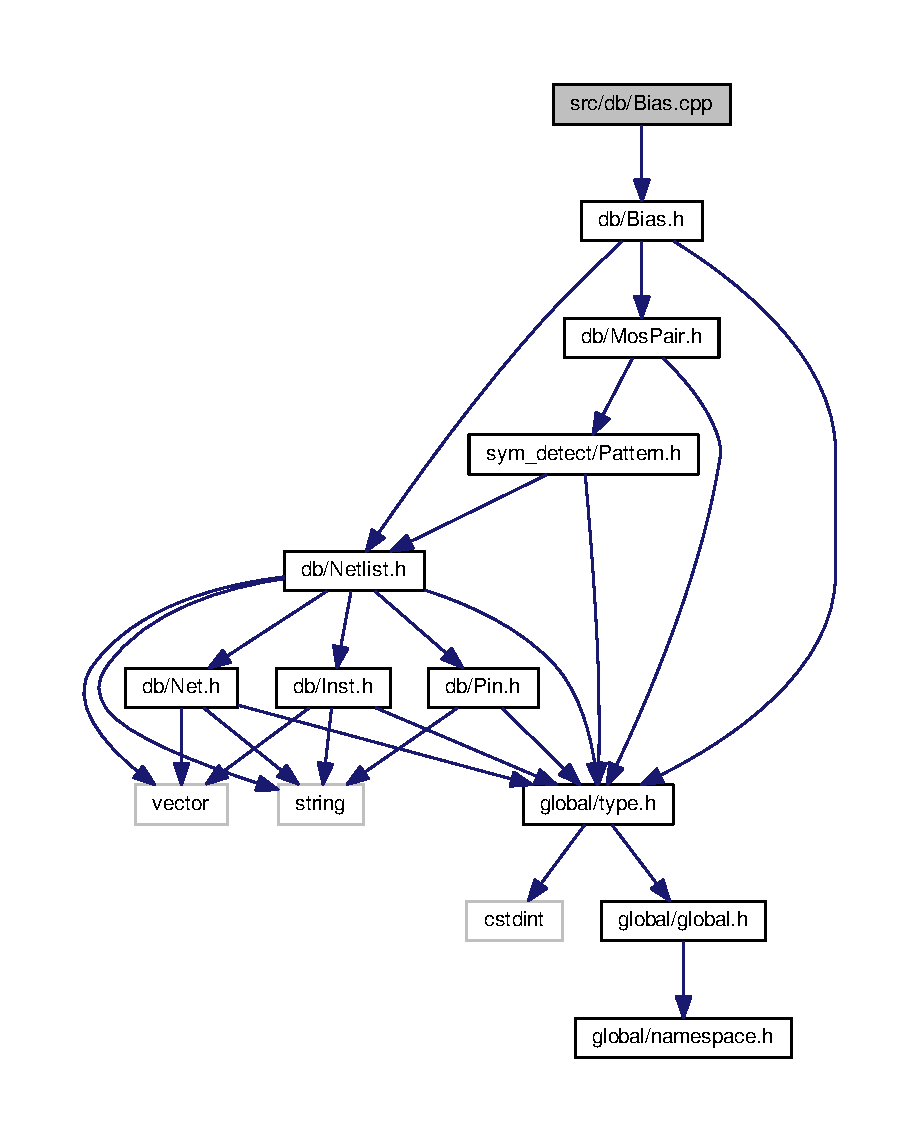
\includegraphics[width=350pt]{Bias_8cpp__incl}
\end{center}
\end{figure}


\subsection{Detailed Description}
\hyperlink{classBias}{Bias} implementation. 

\begin{DoxyAuthor}{Author}
Mingjie Liu 
\end{DoxyAuthor}
\begin{DoxyDate}{Date}
12/11/2018 
\end{DoxyDate}

\hypertarget{Bias_8h}{}\section{src/db/\+Bias.h File Reference}
\label{Bias_8h}\index{src/db/\+Bias.\+h@{src/db/\+Bias.\+h}}


A vector of Mosfet \hyperlink{classBias}{Bias}.  


{\ttfamily \#include \char`\"{}global/type.\+h\char`\"{}}\newline
{\ttfamily \#include \char`\"{}db/\+Netlist.\+h\char`\"{}}\newline
{\ttfamily \#include \char`\"{}db/\+Mos\+Pair.\+h\char`\"{}}\newline
Include dependency graph for Bias.\+h\+:\nopagebreak
\begin{figure}[H]
\begin{center}
\leavevmode
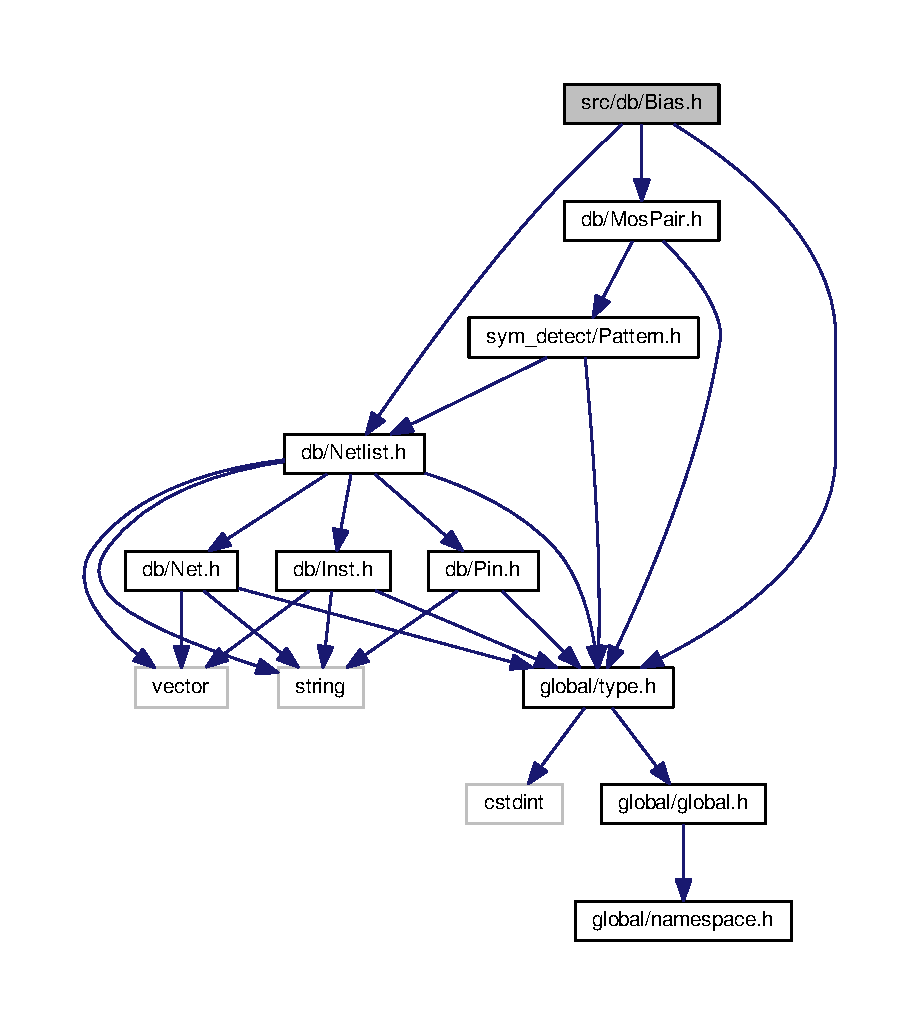
\includegraphics[width=350pt]{Bias_8h__incl}
\end{center}
\end{figure}
This graph shows which files directly or indirectly include this file\+:\nopagebreak
\begin{figure}[H]
\begin{center}
\leavevmode
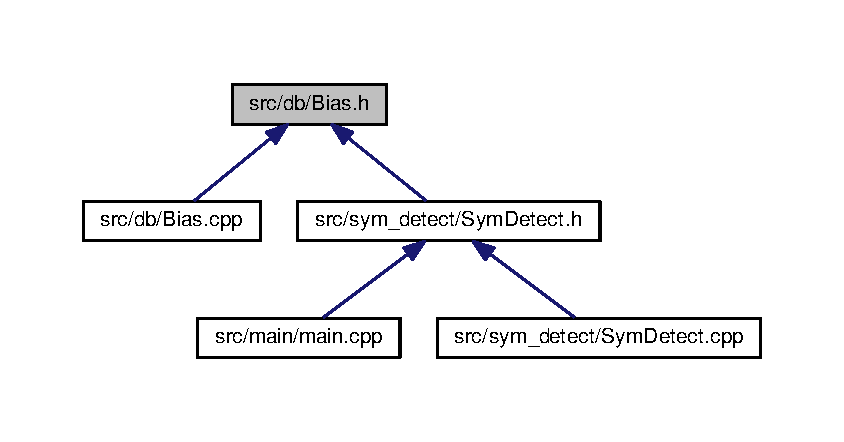
\includegraphics[width=350pt]{Bias_8h__dep__incl}
\end{center}
\end{figure}
\subsection*{Classes}
\begin{DoxyCompactItemize}
\item 
class \hyperlink{classBias}{Bias}
\begin{DoxyCompactList}\small\item\em A vector of Mosfet. \end{DoxyCompactList}\end{DoxyCompactItemize}


\subsection{Detailed Description}
A vector of Mosfet \hyperlink{classBias}{Bias}. 

\begin{DoxyAuthor}{Author}
Mingjie Liu 
\end{DoxyAuthor}
\begin{DoxyDate}{Date}
12/11/2018 
\end{DoxyDate}

\hypertarget{Inst_8h}{}\section{src/db/\+Inst.h File Reference}
\label{Inst_8h}\index{src/db/\+Inst.\+h@{src/db/\+Inst.\+h}}


Instance class.  


{\ttfamily \#include $<$string$>$}\newline
{\ttfamily \#include $<$vector$>$}\newline
{\ttfamily \#include \char`\"{}global/type.\+h\char`\"{}}\newline
Include dependency graph for Inst.\+h\+:\nopagebreak
\begin{figure}[H]
\begin{center}
\leavevmode
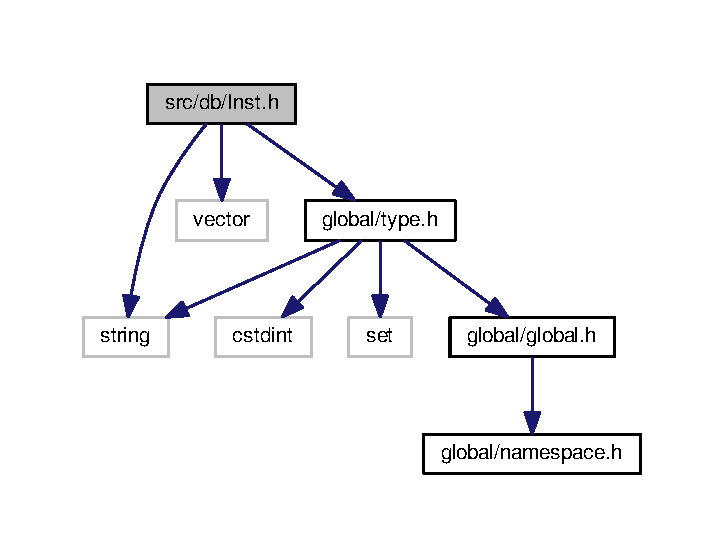
\includegraphics[width=330pt]{Inst_8h__incl}
\end{center}
\end{figure}
This graph shows which files directly or indirectly include this file\+:
\nopagebreak
\begin{figure}[H]
\begin{center}
\leavevmode
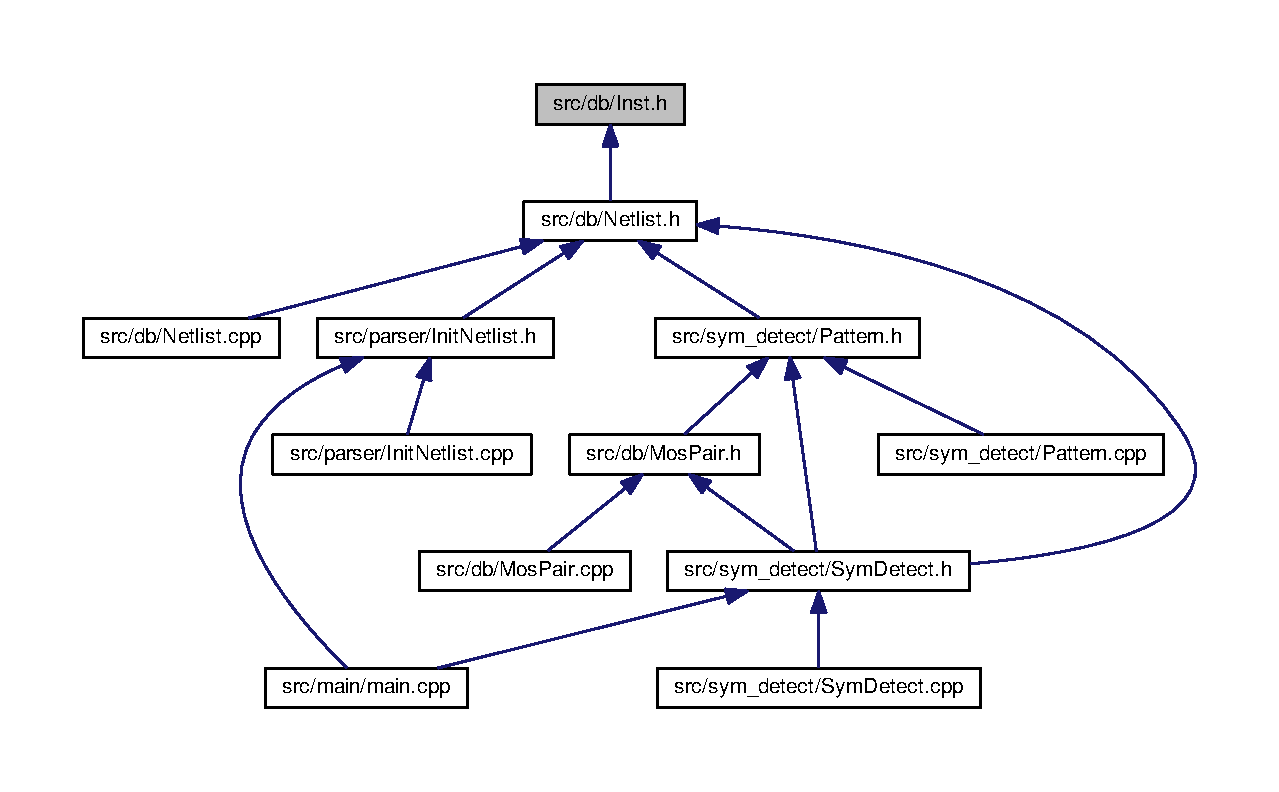
\includegraphics[width=350pt]{Inst_8h__dep__incl}
\end{center}
\end{figure}
\subsection*{Classes}
\begin{DoxyCompactItemize}
\item 
class \hyperlink{classInst}{Inst}
\begin{DoxyCompactList}\small\item\em \hyperlink{classInst}{Inst} class. \end{DoxyCompactList}\end{DoxyCompactItemize}


\subsection{Detailed Description}
Instance class. 

\begin{DoxyAuthor}{Author}
Mingjie Liu 
\end{DoxyAuthor}
\begin{DoxyDate}{Date}
11/24/2018 
\end{DoxyDate}

\hypertarget{MosPair_8cpp}{}\section{src/db/\+Mos\+Pair.cpp File Reference}
\label{MosPair_8cpp}\index{src/db/\+Mos\+Pair.\+cpp@{src/db/\+Mos\+Pair.\+cpp}}


\hyperlink{classMosPair}{Mos\+Pair} implementation.  


{\ttfamily \#include \char`\"{}db/\+Mos\+Pair.\+h\char`\"{}}\newline
Include dependency graph for Mos\+Pair.\+cpp\+:
\nopagebreak
\begin{figure}[H]
\begin{center}
\leavevmode
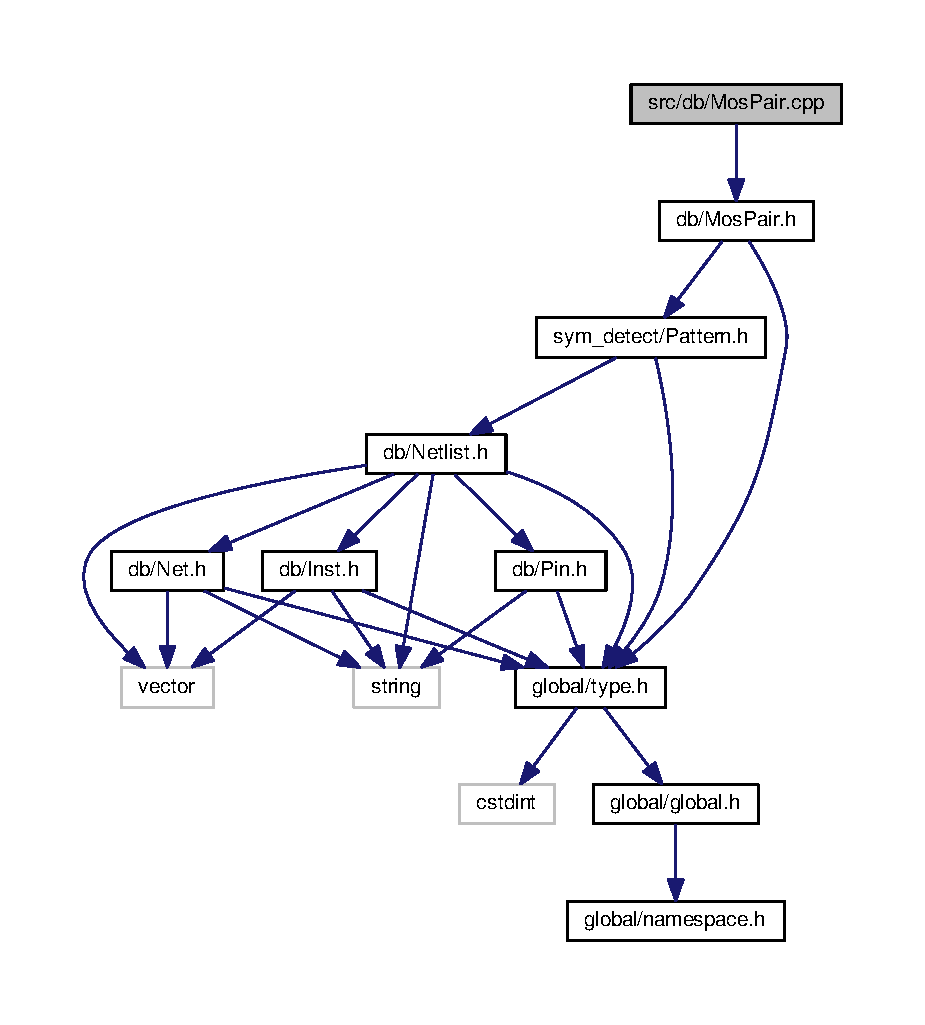
\includegraphics[width=350pt]{MosPair_8cpp__incl}
\end{center}
\end{figure}


\subsection{Detailed Description}
\hyperlink{classMosPair}{Mos\+Pair} implementation. 

\begin{DoxyAuthor}{Author}
Mingjie Liu 
\end{DoxyAuthor}
\begin{DoxyDate}{Date}
11/27/2018 
\end{DoxyDate}

\hypertarget{MosPair_8h}{}\section{src/db/\+Mos\+Pair.h File Reference}
\label{MosPair_8h}\index{src/db/\+Mos\+Pair.\+h@{src/db/\+Mos\+Pair.\+h}}


A pair of Mosfet with Mos\+Pattern.  


{\ttfamily \#include \char`\"{}global/type.\+h\char`\"{}}\newline
{\ttfamily \#include \char`\"{}sym\+\_\+detect/\+Pattern.\+h\char`\"{}}\newline
Include dependency graph for Mos\+Pair.\+h\+:
\nopagebreak
\begin{figure}[H]
\begin{center}
\leavevmode
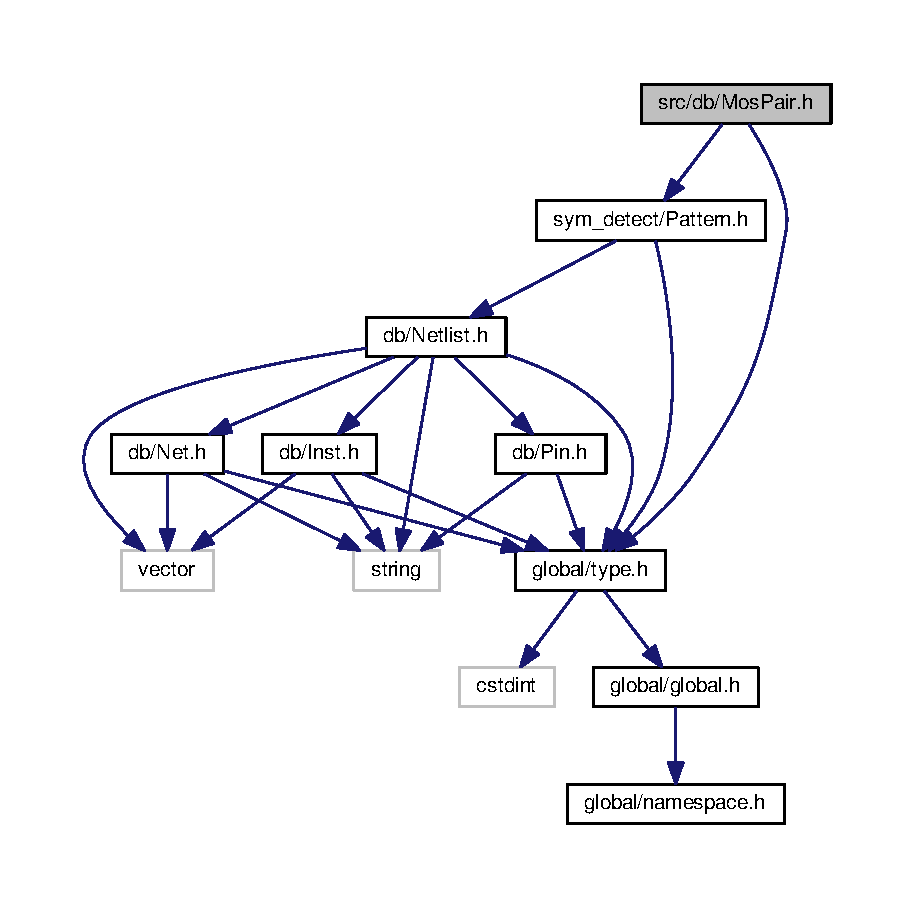
\includegraphics[width=350pt]{MosPair_8h__incl}
\end{center}
\end{figure}
This graph shows which files directly or indirectly include this file\+:
\nopagebreak
\begin{figure}[H]
\begin{center}
\leavevmode
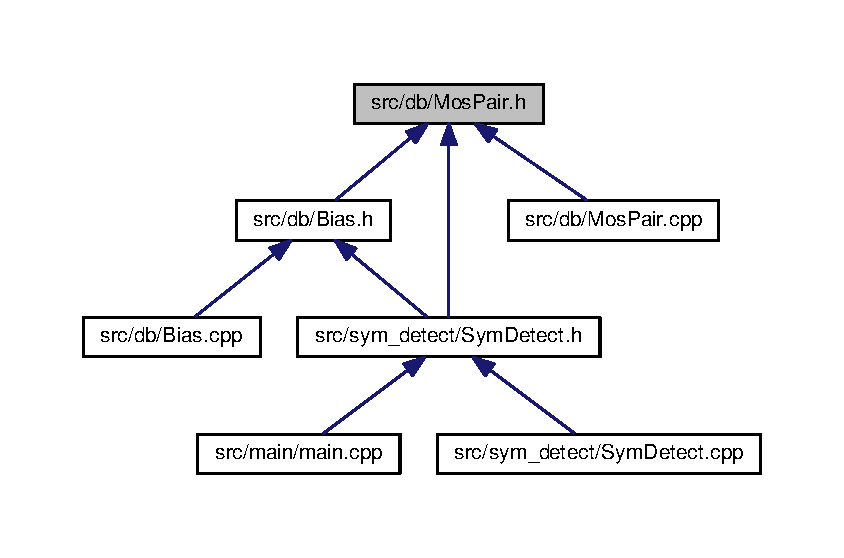
\includegraphics[width=350pt]{MosPair_8h__dep__incl}
\end{center}
\end{figure}
\subsection*{Classes}
\begin{DoxyCompactItemize}
\item 
struct \hyperlink{classMosPair}{Mos\+Pair}
\begin{DoxyCompactList}\small\item\em A pair of Mosfet with Mos\+Pattern. \end{DoxyCompactList}\end{DoxyCompactItemize}


\subsection{Detailed Description}
A pair of Mosfet with Mos\+Pattern. 

\begin{DoxyAuthor}{Author}
Mingjie Liu 
\end{DoxyAuthor}
\begin{DoxyDate}{Date}
11/27/2018 
\end{DoxyDate}

\hypertarget{Net_8cpp}{}\section{src/db/\+Net.cpp File Reference}
\label{Net_8cpp}\index{src/db/\+Net.\+cpp@{src/db/\+Net.\+cpp}}


\hyperlink{classNet}{Net} class implementation.  


{\ttfamily \#include \char`\"{}db/\+Net.\+h\char`\"{}}\newline
{\ttfamily \#include $<$set$>$}\newline
Include dependency graph for Net.\+cpp\+:
\nopagebreak
\begin{figure}[H]
\begin{center}
\leavevmode
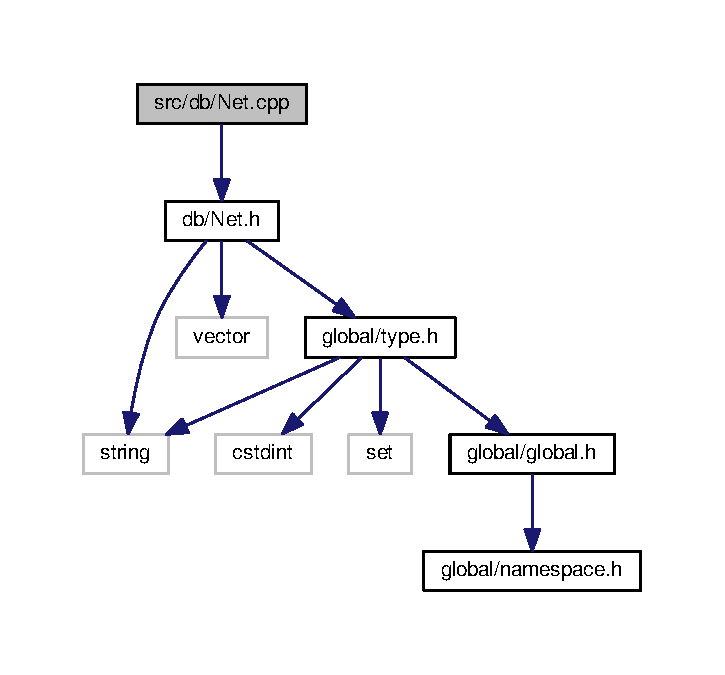
\includegraphics[width=330pt]{Net_8cpp__incl}
\end{center}
\end{figure}
\subsection*{Variables}
\begin{DoxyCompactItemize}
\item 
static \hyperlink{namespace_8h_ae48726a24dab2034454cf6d79e531eb8}{P\+R\+O\+J\+E\+C\+T\+\_\+\+N\+A\+M\+E\+S\+P\+A\+C\+E\+\_\+\+B\+E\+G\+IN} const std\+::set$<$ std\+::string $>$ \hyperlink{Net_8cpp_a0017b2d7dc1a3e4b679679d8d3a07093}{P\+O\+W\+E\+R\+\_\+\+N\+E\+T\+\_\+\+N\+A\+M\+ES} = \{\char`\"{}vdd\char`\"{}, \char`\"{}V\+DD\char`\"{}, \char`\"{}Vdd\char`\"{}, \char`\"{}V\+D\+DA\char`\"{}, \char`\"{}vdda\char`\"{}, \char`\"{}Vdda\char`\"{}\}
\item 
static const std\+::set$<$ std\+::string $>$ \hyperlink{Net_8cpp_ac01f404bd0554d27057520b5637f68b1}{G\+R\+O\+U\+N\+D\+\_\+\+N\+E\+T\+\_\+\+N\+A\+M\+ES} = \{\char`\"{}vss\char`\"{}, \char`\"{}V\+SS\char`\"{}, \char`\"{}Vss\char`\"{}, \char`\"{}V\+S\+SA\char`\"{}, \char`\"{}vssa\char`\"{}, \char`\"{}Vssa\char`\"{}, \char`\"{}gnd\char`\"{}, \char`\"{}Gnd\char`\"{}, \char`\"{}G\+ND\char`\"{}\}
\end{DoxyCompactItemize}


\subsection{Detailed Description}
\hyperlink{classNet}{Net} class implementation. 

\begin{DoxyAuthor}{Author}
Mingjie Liu 
\end{DoxyAuthor}
\begin{DoxyDate}{Date}
11/24/2018 
\end{DoxyDate}


\subsection{Variable Documentation}
\mbox{\Hypertarget{Net_8cpp_ac01f404bd0554d27057520b5637f68b1}\label{Net_8cpp_ac01f404bd0554d27057520b5637f68b1}} 
\index{Net.\+cpp@{Net.\+cpp}!G\+R\+O\+U\+N\+D\+\_\+\+N\+E\+T\+\_\+\+N\+A\+M\+ES@{G\+R\+O\+U\+N\+D\+\_\+\+N\+E\+T\+\_\+\+N\+A\+M\+ES}}
\index{G\+R\+O\+U\+N\+D\+\_\+\+N\+E\+T\+\_\+\+N\+A\+M\+ES@{G\+R\+O\+U\+N\+D\+\_\+\+N\+E\+T\+\_\+\+N\+A\+M\+ES}!Net.\+cpp@{Net.\+cpp}}
\subsubsection{\texorpdfstring{G\+R\+O\+U\+N\+D\+\_\+\+N\+E\+T\+\_\+\+N\+A\+M\+ES}{GROUND\_NET\_NAMES}}
{\footnotesize\ttfamily const std\+::set$<$std\+::string$>$ G\+R\+O\+U\+N\+D\+\_\+\+N\+E\+T\+\_\+\+N\+A\+M\+ES = \{\char`\"{}vss\char`\"{}, \char`\"{}V\+SS\char`\"{}, \char`\"{}Vss\char`\"{}, \char`\"{}V\+S\+SA\char`\"{}, \char`\"{}vssa\char`\"{}, \char`\"{}Vssa\char`\"{}, \char`\"{}gnd\char`\"{}, \char`\"{}Gnd\char`\"{}, \char`\"{}G\+ND\char`\"{}\}\hspace{0.3cm}{\ttfamily [static]}}

A set of possible ground net names. \mbox{\Hypertarget{Net_8cpp_a0017b2d7dc1a3e4b679679d8d3a07093}\label{Net_8cpp_a0017b2d7dc1a3e4b679679d8d3a07093}} 
\index{Net.\+cpp@{Net.\+cpp}!P\+O\+W\+E\+R\+\_\+\+N\+E\+T\+\_\+\+N\+A\+M\+ES@{P\+O\+W\+E\+R\+\_\+\+N\+E\+T\+\_\+\+N\+A\+M\+ES}}
\index{P\+O\+W\+E\+R\+\_\+\+N\+E\+T\+\_\+\+N\+A\+M\+ES@{P\+O\+W\+E\+R\+\_\+\+N\+E\+T\+\_\+\+N\+A\+M\+ES}!Net.\+cpp@{Net.\+cpp}}
\subsubsection{\texorpdfstring{P\+O\+W\+E\+R\+\_\+\+N\+E\+T\+\_\+\+N\+A\+M\+ES}{POWER\_NET\_NAMES}}
{\footnotesize\ttfamily \hyperlink{namespace_8h_ae48726a24dab2034454cf6d79e531eb8}{P\+R\+O\+J\+E\+C\+T\+\_\+\+N\+A\+M\+E\+S\+P\+A\+C\+E\+\_\+\+B\+E\+G\+IN} const std\+::set$<$std\+::string$>$ P\+O\+W\+E\+R\+\_\+\+N\+E\+T\+\_\+\+N\+A\+M\+ES = \{\char`\"{}vdd\char`\"{}, \char`\"{}V\+DD\char`\"{}, \char`\"{}Vdd\char`\"{}, \char`\"{}V\+D\+DA\char`\"{}, \char`\"{}vdda\char`\"{}, \char`\"{}Vdda\char`\"{}\}\hspace{0.3cm}{\ttfamily [static]}}

A set of possible power net names. 
\hypertarget{Net_8h}{}\section{src/db/\+Net.h File Reference}
\label{Net_8h}\index{src/db/\+Net.\+h@{src/db/\+Net.\+h}}


\hyperlink{classNet}{Net} class.  


{\ttfamily \#include $<$string$>$}\newline
{\ttfamily \#include $<$vector$>$}\newline
{\ttfamily \#include \char`\"{}global/type.\+h\char`\"{}}\newline
Include dependency graph for Net.\+h\+:\nopagebreak
\begin{figure}[H]
\begin{center}
\leavevmode
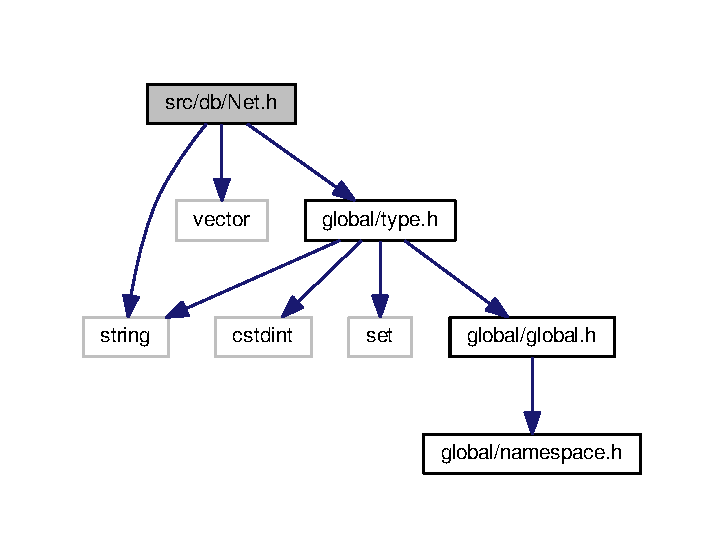
\includegraphics[width=330pt]{Net_8h__incl}
\end{center}
\end{figure}
This graph shows which files directly or indirectly include this file\+:
\nopagebreak
\begin{figure}[H]
\begin{center}
\leavevmode
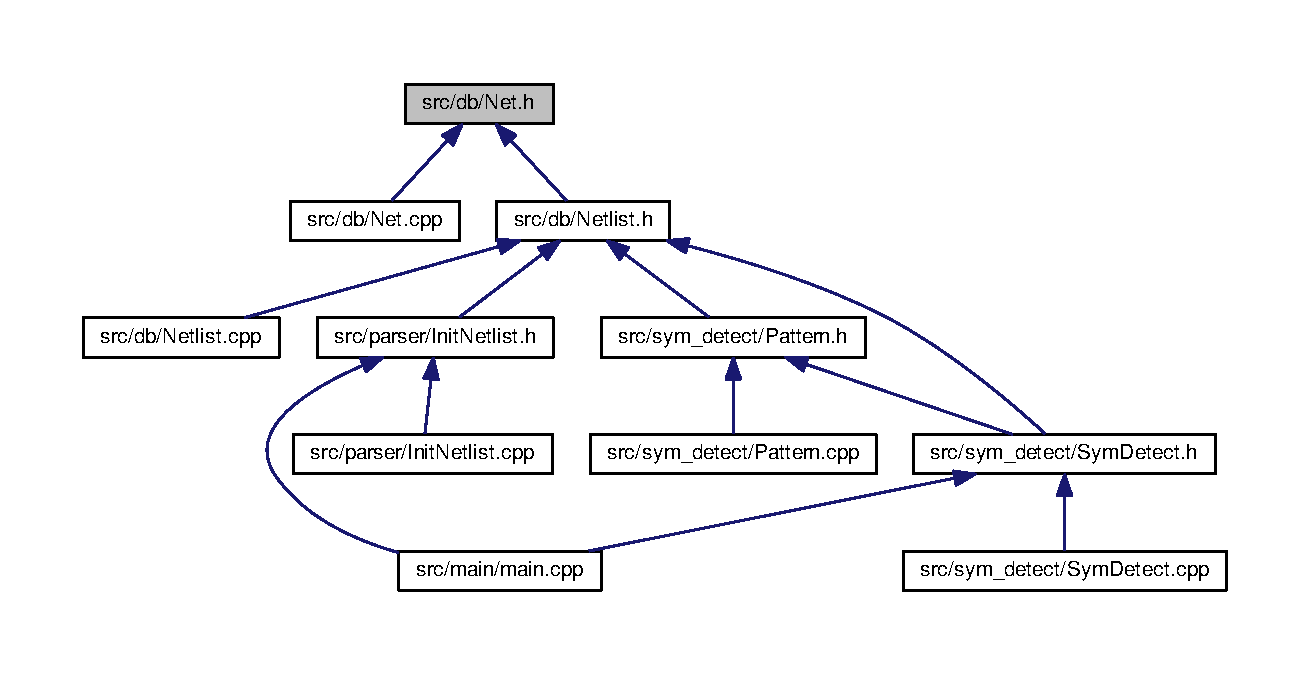
\includegraphics[width=350pt]{Net_8h__dep__incl}
\end{center}
\end{figure}
\subsection*{Classes}
\begin{DoxyCompactItemize}
\item 
class \hyperlink{classNet}{Net}
\begin{DoxyCompactList}\small\item\em \hyperlink{classNet}{Net} class. \end{DoxyCompactList}\end{DoxyCompactItemize}


\subsection{Detailed Description}
\hyperlink{classNet}{Net} class. 

\begin{DoxyAuthor}{Author}
Mingjie L\+Iu 
\end{DoxyAuthor}
\begin{DoxyDate}{Date}
11/24/2018 
\end{DoxyDate}

\hypertarget{Netlist_8cpp}{}\section{src/db/\+Netlist.cpp File Reference}
\label{Netlist_8cpp}\index{src/db/\+Netlist.\+cpp@{src/db/\+Netlist.\+cpp}}


\hyperlink{classNetlist}{Netlist} class implementation.  


{\ttfamily \#include \char`\"{}db/\+Netlist.\+h\char`\"{}}\newline
{\ttfamily \#include $<$algorithm$>$}\newline
Include dependency graph for Netlist.\+cpp\+:
\nopagebreak
\begin{figure}[H]
\begin{center}
\leavevmode
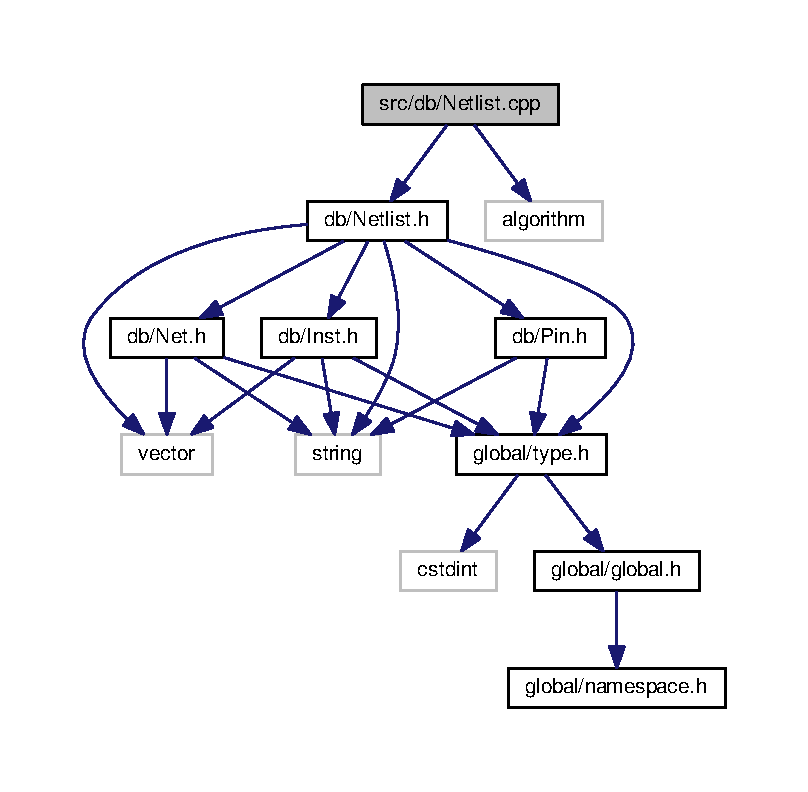
\includegraphics[width=350pt]{Netlist_8cpp__incl}
\end{center}
\end{figure}
\subsection*{Variables}
\begin{DoxyCompactItemize}
\item 
static \hyperlink{namespace_8h_ae48726a24dab2034454cf6d79e531eb8}{P\+R\+O\+J\+E\+C\+T\+\_\+\+N\+A\+M\+E\+S\+P\+A\+C\+E\+\_\+\+B\+E\+G\+IN} const \hyperlink{type_8h_afaab50027002ecbb6c8ac27e727d1bb4}{Pin\+Type} \hyperlink{Netlist_8cpp_a118f5925cbfa27226f61a4af77a208dd}{M\+O\+S\+\_\+\+P\+I\+N\+\_\+\+T\+Y\+PE} \mbox{[}4\mbox{]} = \{\hyperlink{type_8h_afaab50027002ecbb6c8ac27e727d1bb4ad22e8f7ce637479aeffe9dab9ee7337d}{Pin\+Type\+::\+D\+R\+A\+IN}, \hyperlink{type_8h_afaab50027002ecbb6c8ac27e727d1bb4a1818cedf1c2bed8c63664cc8313b443c}{Pin\+Type\+::\+G\+A\+TE}, \hyperlink{type_8h_afaab50027002ecbb6c8ac27e727d1bb4ae60b4854b44ccfb2d92aa6f035171bb4}{Pin\+Type\+::\+S\+O\+U\+R\+CE}, \hyperlink{type_8h_afaab50027002ecbb6c8ac27e727d1bb4a6d5b457ed4205e7f1144ef21b944e552}{Pin\+Type\+::\+B\+U\+LK}\}
\begin{DoxyCompactList}\small\item\em Mos \hyperlink{classPin}{Pin} Types. \end{DoxyCompactList}\item 
static const \hyperlink{type_8h_afaab50027002ecbb6c8ac27e727d1bb4}{Pin\+Type} \hyperlink{Netlist_8cpp_a636b0df3557ae3ac206f153c77ad4e54}{R\+E\+S\+\_\+\+P\+I\+N\+\_\+\+T\+Y\+PE} \mbox{[}3\mbox{]} = \{\hyperlink{type_8h_afaab50027002ecbb6c8ac27e727d1bb4ac9f869114804f0a61ce9b03def9d71f5}{Pin\+Type\+::\+T\+H\+IS}, \hyperlink{type_8h_afaab50027002ecbb6c8ac27e727d1bb4a13d613e84b1e7d08d869695a750caf23}{Pin\+Type\+::\+T\+H\+AT}, \hyperlink{type_8h_a53644c687d6bc203d9d3d3ee70075f61a03570470bad94692ce93e32700d2e1cb}{Pin\+Type\+::\+O\+T\+H\+ER}\}
\begin{DoxyCompactList}\small\item\em Res/\+Cap \hyperlink{classPin}{Pin} Types. \end{DoxyCompactList}\end{DoxyCompactItemize}


\subsection{Detailed Description}
\hyperlink{classNetlist}{Netlist} class implementation. 

\begin{DoxyAuthor}{Author}
Mingjie Liu 
\end{DoxyAuthor}
\begin{DoxyDate}{Date}
11/24/2018 
\end{DoxyDate}


\subsection{Variable Documentation}
\mbox{\Hypertarget{Netlist_8cpp_a118f5925cbfa27226f61a4af77a208dd}\label{Netlist_8cpp_a118f5925cbfa27226f61a4af77a208dd}} 
\index{Netlist.\+cpp@{Netlist.\+cpp}!M\+O\+S\+\_\+\+P\+I\+N\+\_\+\+T\+Y\+PE@{M\+O\+S\+\_\+\+P\+I\+N\+\_\+\+T\+Y\+PE}}
\index{M\+O\+S\+\_\+\+P\+I\+N\+\_\+\+T\+Y\+PE@{M\+O\+S\+\_\+\+P\+I\+N\+\_\+\+T\+Y\+PE}!Netlist.\+cpp@{Netlist.\+cpp}}
\subsubsection{\texorpdfstring{M\+O\+S\+\_\+\+P\+I\+N\+\_\+\+T\+Y\+PE}{MOS\_PIN\_TYPE}}
{\footnotesize\ttfamily \hyperlink{namespace_8h_ae48726a24dab2034454cf6d79e531eb8}{P\+R\+O\+J\+E\+C\+T\+\_\+\+N\+A\+M\+E\+S\+P\+A\+C\+E\+\_\+\+B\+E\+G\+IN} const \hyperlink{type_8h_afaab50027002ecbb6c8ac27e727d1bb4}{Pin\+Type} M\+O\+S\+\_\+\+P\+I\+N\+\_\+\+T\+Y\+PE\mbox{[}4\mbox{]} = \{\hyperlink{type_8h_afaab50027002ecbb6c8ac27e727d1bb4ad22e8f7ce637479aeffe9dab9ee7337d}{Pin\+Type\+::\+D\+R\+A\+IN}, \hyperlink{type_8h_afaab50027002ecbb6c8ac27e727d1bb4a1818cedf1c2bed8c63664cc8313b443c}{Pin\+Type\+::\+G\+A\+TE}, \hyperlink{type_8h_afaab50027002ecbb6c8ac27e727d1bb4ae60b4854b44ccfb2d92aa6f035171bb4}{Pin\+Type\+::\+S\+O\+U\+R\+CE}, \hyperlink{type_8h_afaab50027002ecbb6c8ac27e727d1bb4a6d5b457ed4205e7f1144ef21b944e552}{Pin\+Type\+::\+B\+U\+LK}\}\hspace{0.3cm}{\ttfamily [static]}}



Mos \hyperlink{classPin}{Pin} Types. 

\mbox{\Hypertarget{Netlist_8cpp_a636b0df3557ae3ac206f153c77ad4e54}\label{Netlist_8cpp_a636b0df3557ae3ac206f153c77ad4e54}} 
\index{Netlist.\+cpp@{Netlist.\+cpp}!R\+E\+S\+\_\+\+P\+I\+N\+\_\+\+T\+Y\+PE@{R\+E\+S\+\_\+\+P\+I\+N\+\_\+\+T\+Y\+PE}}
\index{R\+E\+S\+\_\+\+P\+I\+N\+\_\+\+T\+Y\+PE@{R\+E\+S\+\_\+\+P\+I\+N\+\_\+\+T\+Y\+PE}!Netlist.\+cpp@{Netlist.\+cpp}}
\subsubsection{\texorpdfstring{R\+E\+S\+\_\+\+P\+I\+N\+\_\+\+T\+Y\+PE}{RES\_PIN\_TYPE}}
{\footnotesize\ttfamily const \hyperlink{type_8h_afaab50027002ecbb6c8ac27e727d1bb4}{Pin\+Type} R\+E\+S\+\_\+\+P\+I\+N\+\_\+\+T\+Y\+PE\mbox{[}3\mbox{]} = \{\hyperlink{type_8h_afaab50027002ecbb6c8ac27e727d1bb4ac9f869114804f0a61ce9b03def9d71f5}{Pin\+Type\+::\+T\+H\+IS}, \hyperlink{type_8h_afaab50027002ecbb6c8ac27e727d1bb4a13d613e84b1e7d08d869695a750caf23}{Pin\+Type\+::\+T\+H\+AT}, \hyperlink{type_8h_a53644c687d6bc203d9d3d3ee70075f61a03570470bad94692ce93e32700d2e1cb}{Pin\+Type\+::\+O\+T\+H\+ER}\}\hspace{0.3cm}{\ttfamily [static]}}



Res/\+Cap \hyperlink{classPin}{Pin} Types. 


\hypertarget{Netlist_8h}{}\section{src/db/\+Netlist.h File Reference}
\label{Netlist_8h}\index{src/db/\+Netlist.\+h@{src/db/\+Netlist.\+h}}


\hyperlink{classNetlist}{Netlist} class.  


{\ttfamily \#include $<$vector$>$}\newline
{\ttfamily \#include $<$string$>$}\newline
{\ttfamily \#include \char`\"{}global/type.\+h\char`\"{}}\newline
{\ttfamily \#include \char`\"{}db/\+Net.\+h\char`\"{}}\newline
{\ttfamily \#include \char`\"{}db/\+Pin.\+h\char`\"{}}\newline
{\ttfamily \#include \char`\"{}db/\+Inst.\+h\char`\"{}}\newline
Include dependency graph for Netlist.\+h\+:\nopagebreak
\begin{figure}[H]
\begin{center}
\leavevmode
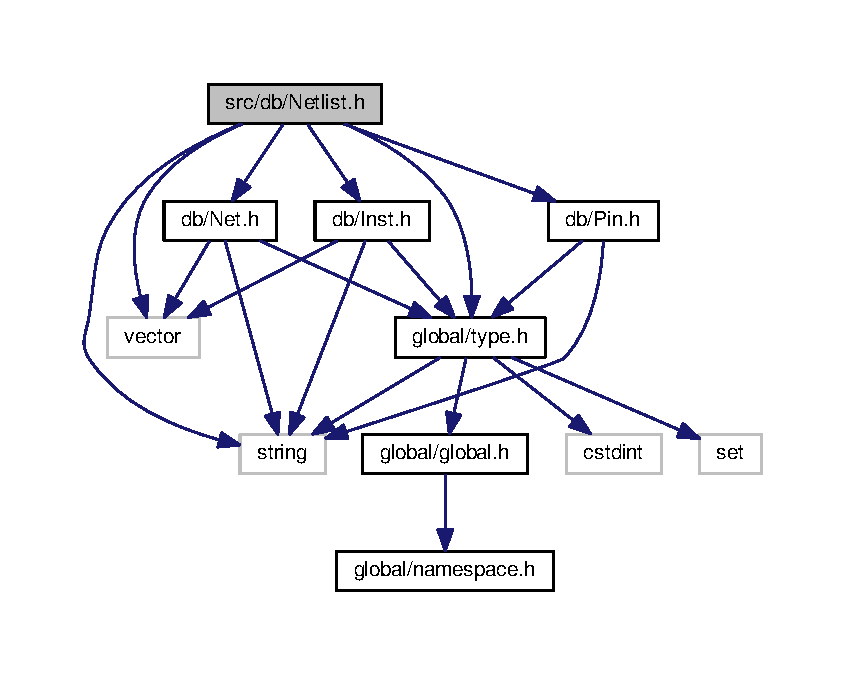
\includegraphics[width=350pt]{Netlist_8h__incl}
\end{center}
\end{figure}
This graph shows which files directly or indirectly include this file\+:
\nopagebreak
\begin{figure}[H]
\begin{center}
\leavevmode
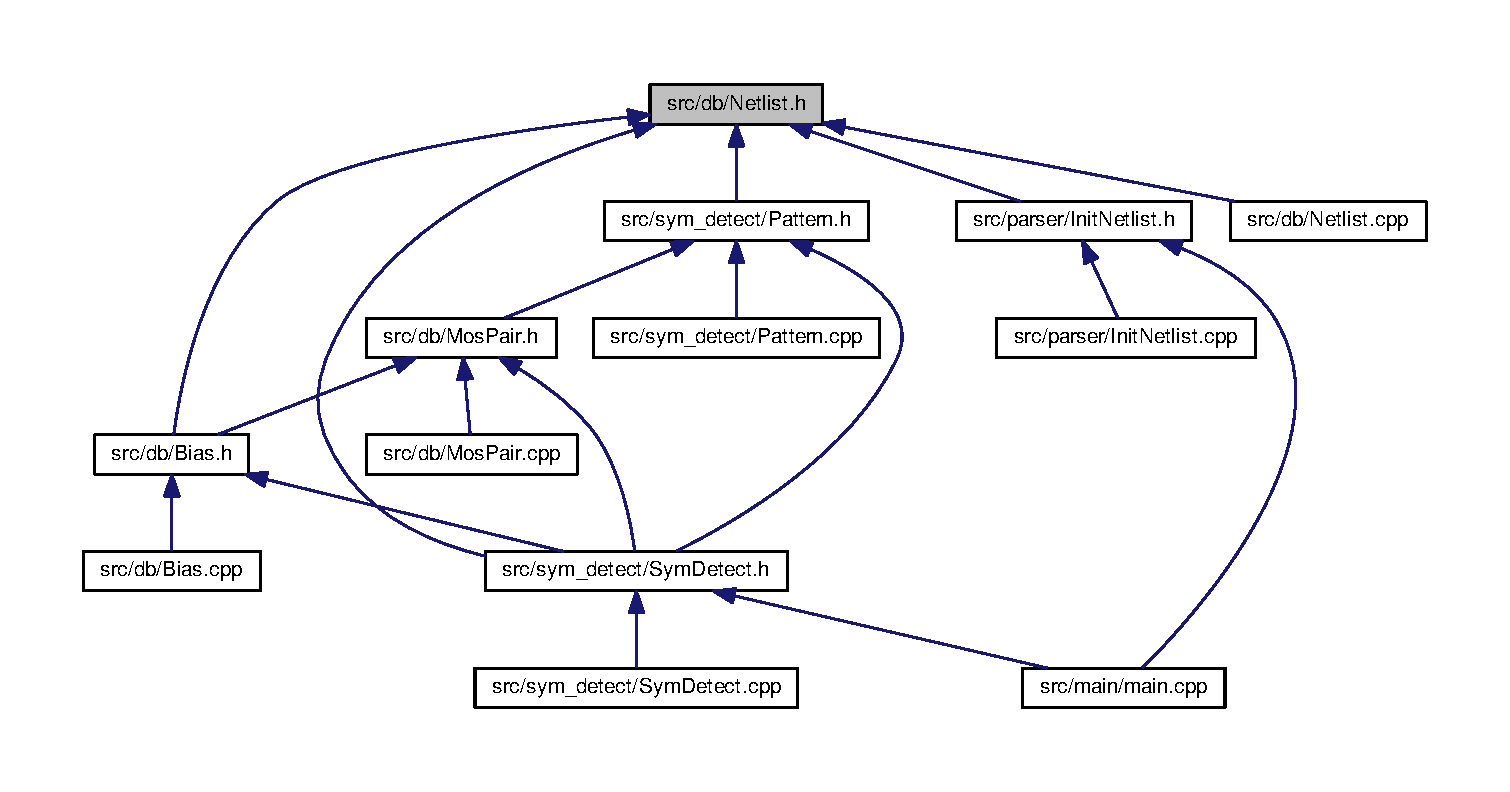
\includegraphics[width=350pt]{Netlist_8h__dep__incl}
\end{center}
\end{figure}
\subsection*{Classes}
\begin{DoxyCompactItemize}
\item 
class \hyperlink{classNetlist}{Netlist}
\begin{DoxyCompactList}\small\item\em \hyperlink{classNetlist}{Netlist} class. \end{DoxyCompactList}\item 
struct \hyperlink{structNetlist_1_1InitNet}{Netlist\+::\+Init\+Net}
\begin{DoxyCompactList}\small\item\em \hyperlink{classNet}{Net} for instantiation. \end{DoxyCompactList}\item 
struct \hyperlink{structNetlist_1_1InitInst}{Netlist\+::\+Init\+Inst}
\begin{DoxyCompactList}\small\item\em \hyperlink{classInst}{Inst} for instantiation. \end{DoxyCompactList}\item 
struct \hyperlink{structNetlist_1_1InitDataObj}{Netlist\+::\+Init\+Data\+Obj}
\begin{DoxyCompactList}\small\item\em Instantiate \hyperlink{classNetlist}{Netlist} class. \end{DoxyCompactList}\end{DoxyCompactItemize}


\subsection{Detailed Description}
\hyperlink{classNetlist}{Netlist} class. 

\begin{DoxyAuthor}{Author}
Mingjie Liu 
\end{DoxyAuthor}
\begin{DoxyDate}{Date}
11/24/2018 
\end{DoxyDate}

\hypertarget{NetPair_8h}{}\section{src/db/\+Net\+Pair.h File Reference}
\label{NetPair_8h}\index{src/db/\+Net\+Pair.\+h@{src/db/\+Net\+Pair.\+h}}


A pair of symmetry nets.  


{\ttfamily \#include \char`\"{}global/type.\+h\char`\"{}}\newline
Include dependency graph for Net\+Pair.\+h\+:\nopagebreak
\begin{figure}[H]
\begin{center}
\leavevmode
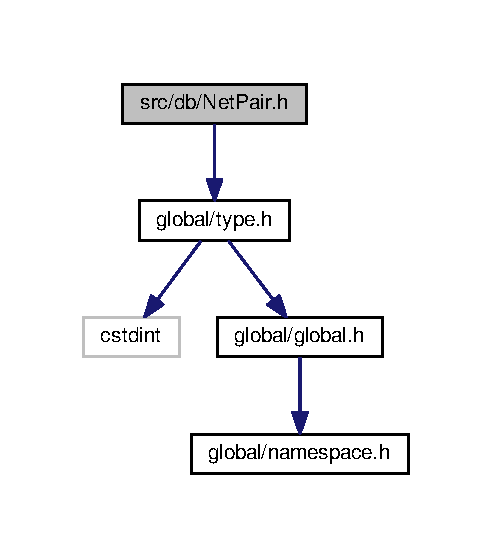
\includegraphics[width=236pt]{NetPair_8h__incl}
\end{center}
\end{figure}
This graph shows which files directly or indirectly include this file\+:\nopagebreak
\begin{figure}[H]
\begin{center}
\leavevmode
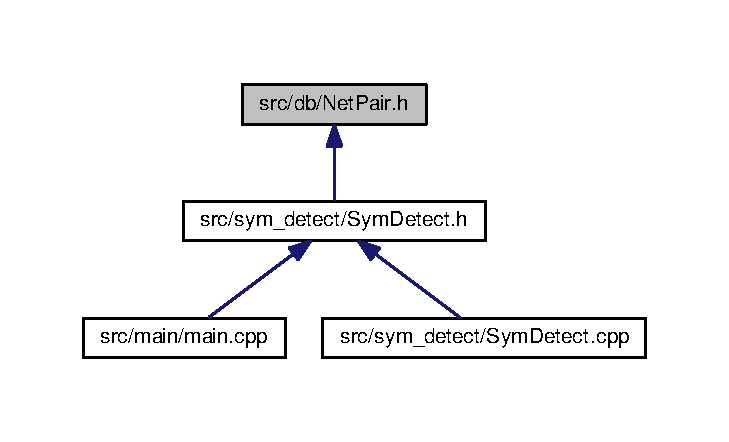
\includegraphics[width=350pt]{NetPair_8h__dep__incl}
\end{center}
\end{figure}
\subsection*{Classes}
\begin{DoxyCompactItemize}
\item 
class \hyperlink{classNetPair}{Net\+Pair}
\begin{DoxyCompactList}\small\item\em A pair of \hyperlink{classNet}{Net} that are symmetric. \end{DoxyCompactList}\end{DoxyCompactItemize}


\subsection{Detailed Description}
A pair of symmetry nets. 

\begin{DoxyAuthor}{Author}
Mingjie Liu 
\end{DoxyAuthor}
\begin{DoxyDate}{Date}
12/06/2018 
\end{DoxyDate}

\hypertarget{Pin_8cpp}{}\section{src/db/\+Pin.cpp File Reference}
\label{Pin_8cpp}\index{src/db/\+Pin.\+cpp@{src/db/\+Pin.\+cpp}}


\hyperlink{classNet}{Net} class implementation.  


{\ttfamily \#include \char`\"{}db/\+Pin.\+h\char`\"{}}\newline
Include dependency graph for Pin.\+cpp\+:\nopagebreak
\begin{figure}[H]
\begin{center}
\leavevmode
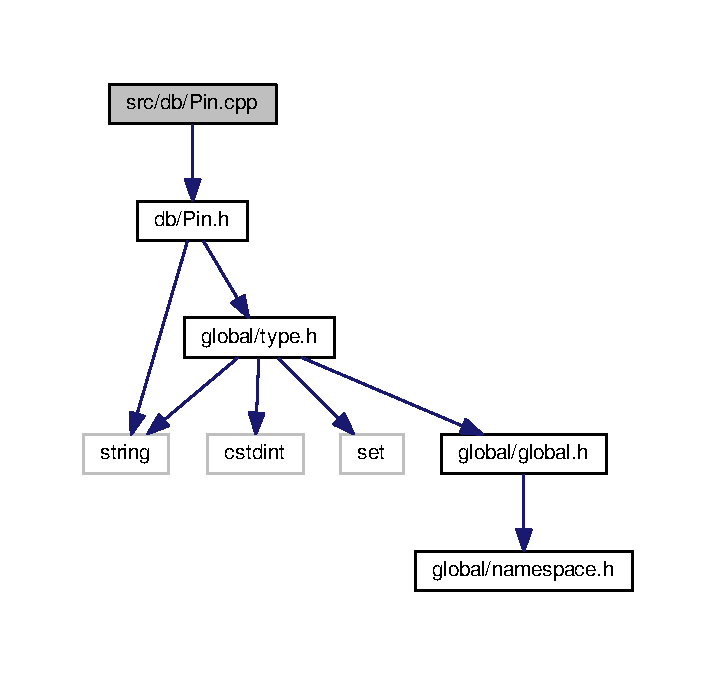
\includegraphics[width=269pt]{Pin_8cpp__incl}
\end{center}
\end{figure}


\subsection{Detailed Description}
\hyperlink{classNet}{Net} class implementation. 

\begin{DoxyAuthor}{Author}
Mingjie Liu 
\end{DoxyAuthor}
\begin{DoxyDate}{Date}
11/24/2018 
\end{DoxyDate}

\hypertarget{Pin_8h}{}\section{src/db/\+Pin.h File Reference}
\label{Pin_8h}\index{src/db/\+Pin.\+h@{src/db/\+Pin.\+h}}


\hyperlink{classPin}{Pin} class.  


{\ttfamily \#include $<$string$>$}\newline
{\ttfamily \#include \char`\"{}global/type.\+h\char`\"{}}\newline
Include dependency graph for Pin.\+h\+:\nopagebreak
\begin{figure}[H]
\begin{center}
\leavevmode
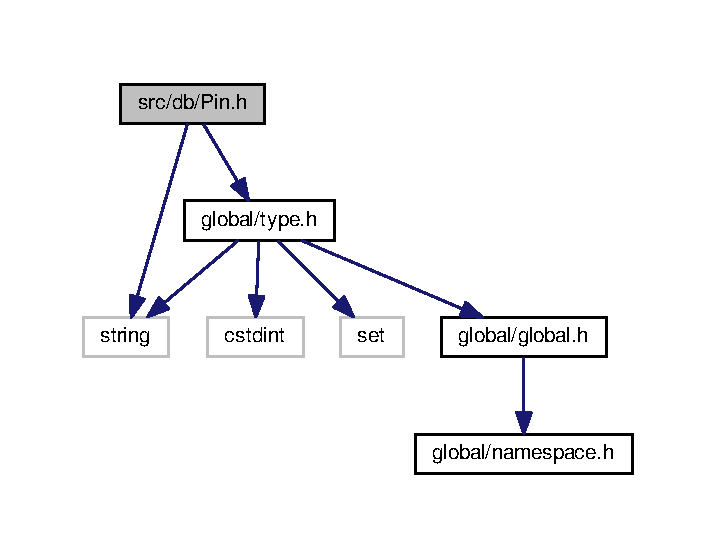
\includegraphics[width=269pt]{Pin_8h__incl}
\end{center}
\end{figure}
This graph shows which files directly or indirectly include this file\+:\nopagebreak
\begin{figure}[H]
\begin{center}
\leavevmode
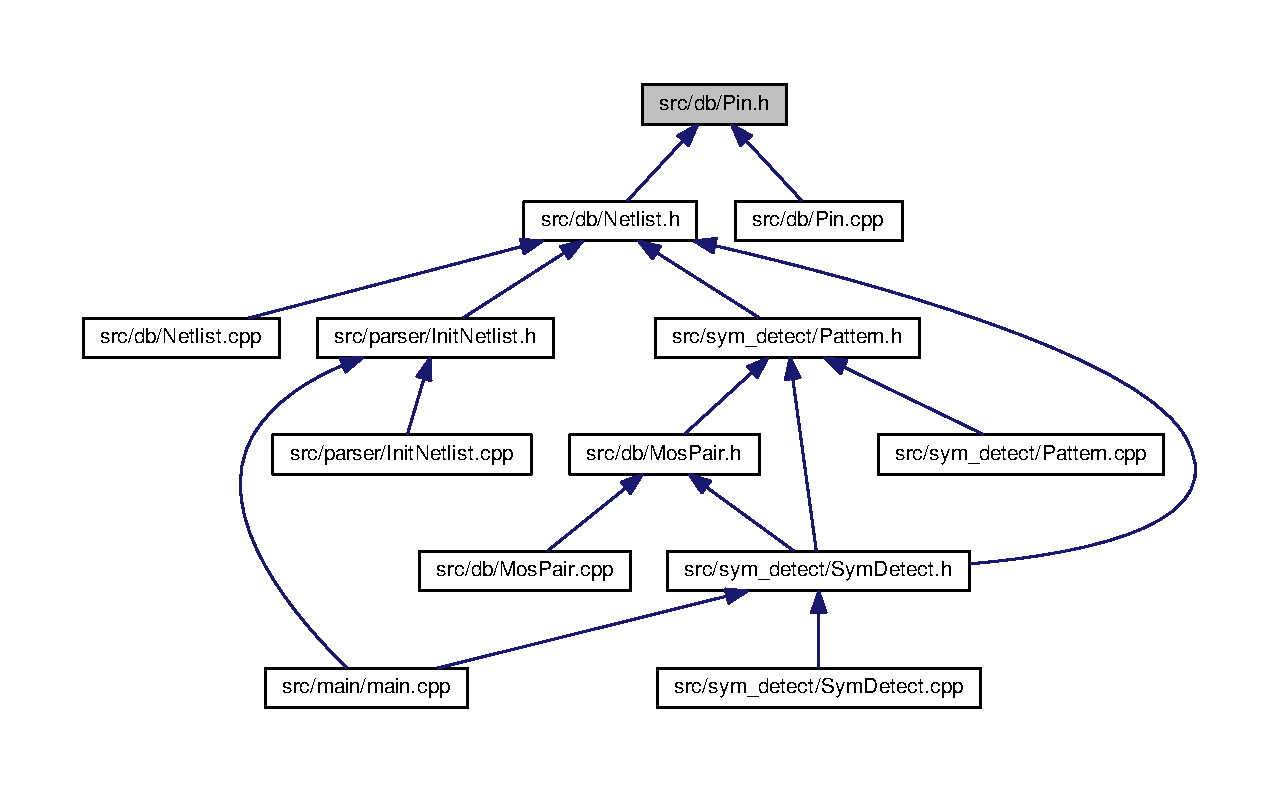
\includegraphics[width=350pt]{Pin_8h__dep__incl}
\end{center}
\end{figure}
\subsection*{Classes}
\begin{DoxyCompactItemize}
\item 
class \hyperlink{classPin}{Pin}
\begin{DoxyCompactList}\small\item\em \hyperlink{classPin}{Pin} class. \end{DoxyCompactList}\end{DoxyCompactItemize}


\subsection{Detailed Description}
\hyperlink{classPin}{Pin} class. 

\begin{DoxyAuthor}{Author}
Mingjie Liu 
\end{DoxyAuthor}
\begin{DoxyDate}{Date}
11/24/2018 
\end{DoxyDate}

\hypertarget{global_8h}{}\section{src/global/global.h File Reference}
\label{global_8h}\index{src/global/global.\+h@{src/global/global.\+h}}


Global header file.  


{\ttfamily \#include \char`\"{}global/namespace.\+h\char`\"{}}\newline
Include dependency graph for global.\+h\+:\nopagebreak
\begin{figure}[H]
\begin{center}
\leavevmode
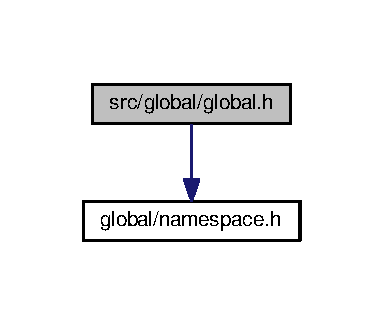
\includegraphics[width=184pt]{global_8h__incl}
\end{center}
\end{figure}
This graph shows which files directly or indirectly include this file\+:\nopagebreak
\begin{figure}[H]
\begin{center}
\leavevmode
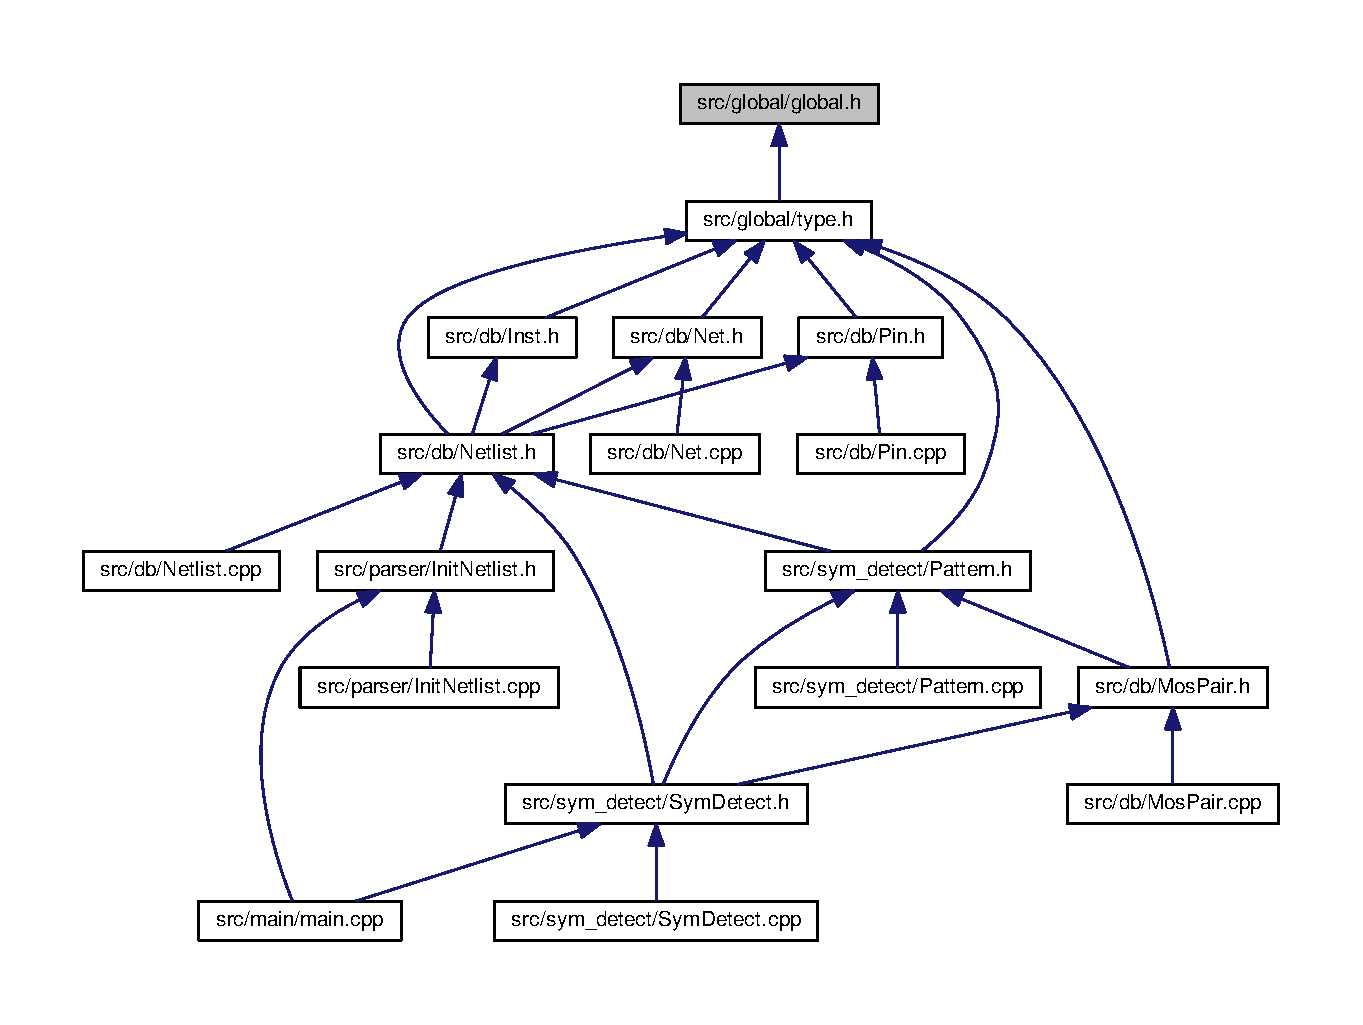
\includegraphics[width=350pt]{global_8h__dep__incl}
\end{center}
\end{figure}


\subsection{Detailed Description}
Global header file. 

\begin{DoxyAuthor}{Author}
Mingjie Liu 
\end{DoxyAuthor}
\begin{DoxyDate}{Date}
11/24/2018 
\end{DoxyDate}

\hypertarget{namespace_8h}{}\section{src/global/namespace.h File Reference}
\label{namespace_8h}\index{src/global/namespace.\+h@{src/global/namespace.\+h}}


Namespace header file.  


This graph shows which files directly or indirectly include this file\+:\nopagebreak
\begin{figure}[H]
\begin{center}
\leavevmode
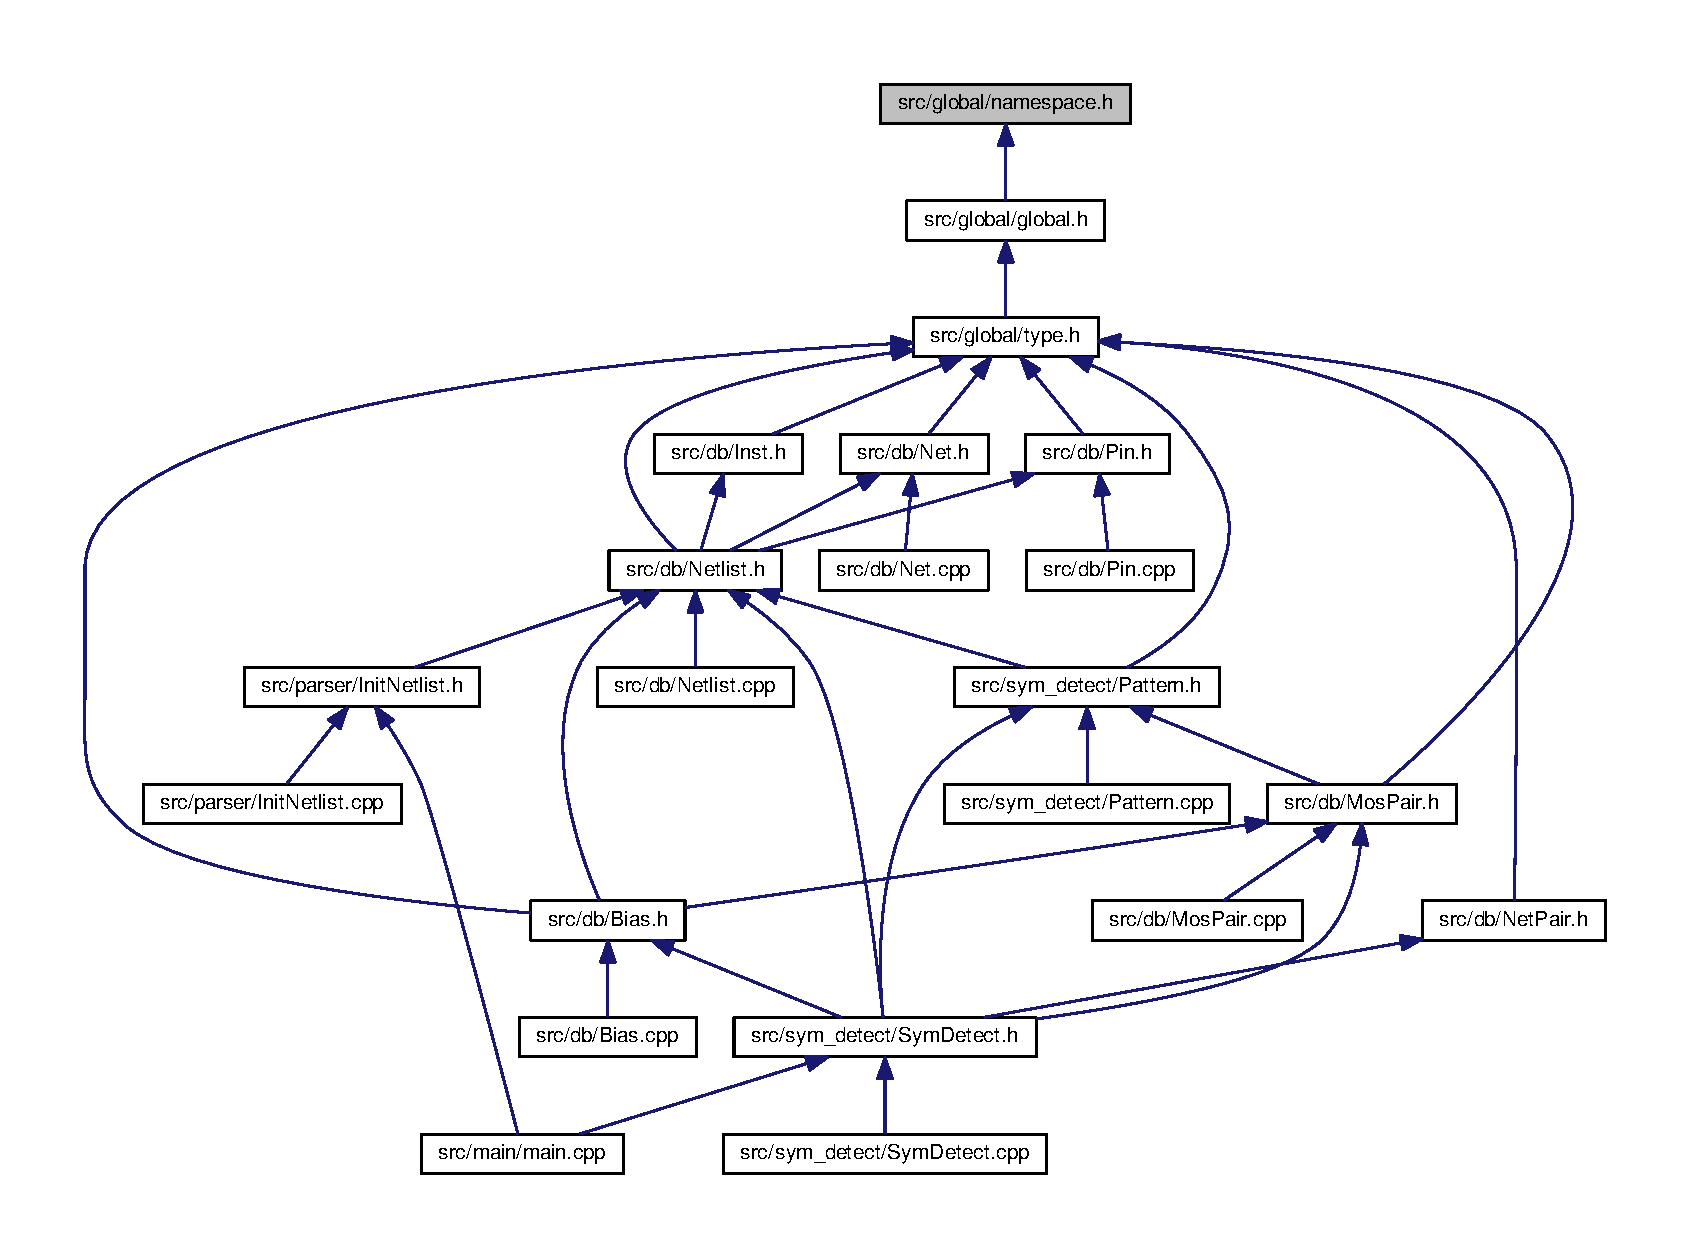
\includegraphics[width=350pt]{namespace_8h__dep__incl}
\end{center}
\end{figure}
\subsection*{Macros}
\begin{DoxyCompactItemize}
\item 
\#define \hyperlink{namespace_8h_ab0be54b8d51fc692e52e8e97f8d01b54}{P\+R\+O\+J\+E\+C\+T\+\_\+\+N\+A\+M\+E\+S\+P\+A\+CE}~S\+FA
\item 
\#define \hyperlink{namespace_8h_ae48726a24dab2034454cf6d79e531eb8}{P\+R\+O\+J\+E\+C\+T\+\_\+\+N\+A\+M\+E\+S\+P\+A\+C\+E\+\_\+\+B\+E\+G\+IN}~namespace \hyperlink{namespace_8h_ab0be54b8d51fc692e52e8e97f8d01b54}{P\+R\+O\+J\+E\+C\+T\+\_\+\+N\+A\+M\+E\+S\+P\+A\+CE} \{
\item 
\#define \hyperlink{namespace_8h_a59165a6be02fced393ec446a4cb22bc7}{P\+R\+O\+J\+E\+C\+T\+\_\+\+N\+A\+M\+E\+S\+P\+A\+C\+E\+\_\+\+E\+ND}~\}
\end{DoxyCompactItemize}


\subsection{Detailed Description}
Namespace header file. 

\begin{DoxyAuthor}{Author}
Mingjie Liu 
\end{DoxyAuthor}
\begin{DoxyDate}{Date}
11/24/2018 
\end{DoxyDate}


\subsection{Macro Definition Documentation}
\mbox{\Hypertarget{namespace_8h_ab0be54b8d51fc692e52e8e97f8d01b54}\label{namespace_8h_ab0be54b8d51fc692e52e8e97f8d01b54}} 
\index{namespace.\+h@{namespace.\+h}!P\+R\+O\+J\+E\+C\+T\+\_\+\+N\+A\+M\+E\+S\+P\+A\+CE@{P\+R\+O\+J\+E\+C\+T\+\_\+\+N\+A\+M\+E\+S\+P\+A\+CE}}
\index{P\+R\+O\+J\+E\+C\+T\+\_\+\+N\+A\+M\+E\+S\+P\+A\+CE@{P\+R\+O\+J\+E\+C\+T\+\_\+\+N\+A\+M\+E\+S\+P\+A\+CE}!namespace.\+h@{namespace.\+h}}
\subsubsection{\texorpdfstring{P\+R\+O\+J\+E\+C\+T\+\_\+\+N\+A\+M\+E\+S\+P\+A\+CE}{PROJECT\_NAMESPACE}}
{\footnotesize\ttfamily \#define P\+R\+O\+J\+E\+C\+T\+\_\+\+N\+A\+M\+E\+S\+P\+A\+CE~S\+FA}

\mbox{\Hypertarget{namespace_8h_ae48726a24dab2034454cf6d79e531eb8}\label{namespace_8h_ae48726a24dab2034454cf6d79e531eb8}} 
\index{namespace.\+h@{namespace.\+h}!P\+R\+O\+J\+E\+C\+T\+\_\+\+N\+A\+M\+E\+S\+P\+A\+C\+E\+\_\+\+B\+E\+G\+IN@{P\+R\+O\+J\+E\+C\+T\+\_\+\+N\+A\+M\+E\+S\+P\+A\+C\+E\+\_\+\+B\+E\+G\+IN}}
\index{P\+R\+O\+J\+E\+C\+T\+\_\+\+N\+A\+M\+E\+S\+P\+A\+C\+E\+\_\+\+B\+E\+G\+IN@{P\+R\+O\+J\+E\+C\+T\+\_\+\+N\+A\+M\+E\+S\+P\+A\+C\+E\+\_\+\+B\+E\+G\+IN}!namespace.\+h@{namespace.\+h}}
\subsubsection{\texorpdfstring{P\+R\+O\+J\+E\+C\+T\+\_\+\+N\+A\+M\+E\+S\+P\+A\+C\+E\+\_\+\+B\+E\+G\+IN}{PROJECT\_NAMESPACE\_BEGIN}}
{\footnotesize\ttfamily \#define P\+R\+O\+J\+E\+C\+T\+\_\+\+N\+A\+M\+E\+S\+P\+A\+C\+E\+\_\+\+B\+E\+G\+IN~namespace \hyperlink{namespace_8h_ab0be54b8d51fc692e52e8e97f8d01b54}{P\+R\+O\+J\+E\+C\+T\+\_\+\+N\+A\+M\+E\+S\+P\+A\+CE} \{}

\mbox{\Hypertarget{namespace_8h_a59165a6be02fced393ec446a4cb22bc7}\label{namespace_8h_a59165a6be02fced393ec446a4cb22bc7}} 
\index{namespace.\+h@{namespace.\+h}!P\+R\+O\+J\+E\+C\+T\+\_\+\+N\+A\+M\+E\+S\+P\+A\+C\+E\+\_\+\+E\+ND@{P\+R\+O\+J\+E\+C\+T\+\_\+\+N\+A\+M\+E\+S\+P\+A\+C\+E\+\_\+\+E\+ND}}
\index{P\+R\+O\+J\+E\+C\+T\+\_\+\+N\+A\+M\+E\+S\+P\+A\+C\+E\+\_\+\+E\+ND@{P\+R\+O\+J\+E\+C\+T\+\_\+\+N\+A\+M\+E\+S\+P\+A\+C\+E\+\_\+\+E\+ND}!namespace.\+h@{namespace.\+h}}
\subsubsection{\texorpdfstring{P\+R\+O\+J\+E\+C\+T\+\_\+\+N\+A\+M\+E\+S\+P\+A\+C\+E\+\_\+\+E\+ND}{PROJECT\_NAMESPACE\_END}}
{\footnotesize\ttfamily \#define P\+R\+O\+J\+E\+C\+T\+\_\+\+N\+A\+M\+E\+S\+P\+A\+C\+E\+\_\+\+E\+ND~\}}


\hypertarget{type_8h}{}\section{src/global/type.h File Reference}
\label{type_8h}\index{src/global/type.\+h@{src/global/type.\+h}}


Type header file.  


{\ttfamily \#include $<$cstdint$>$}\newline
{\ttfamily \#include \char`\"{}global/global.\+h\char`\"{}}\newline
Include dependency graph for type.\+h\+:\nopagebreak
\begin{figure}[H]
\begin{center}
\leavevmode
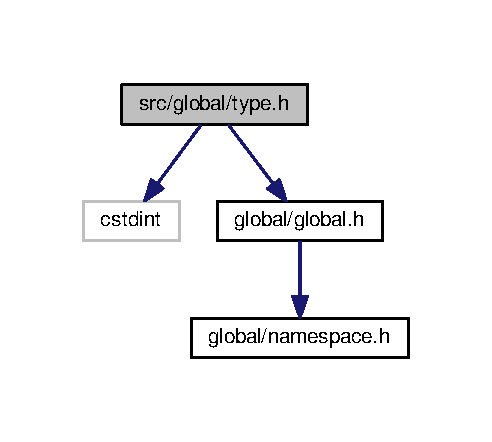
\includegraphics[width=236pt]{type_8h__incl}
\end{center}
\end{figure}
This graph shows which files directly or indirectly include this file\+:
\nopagebreak
\begin{figure}[H]
\begin{center}
\leavevmode
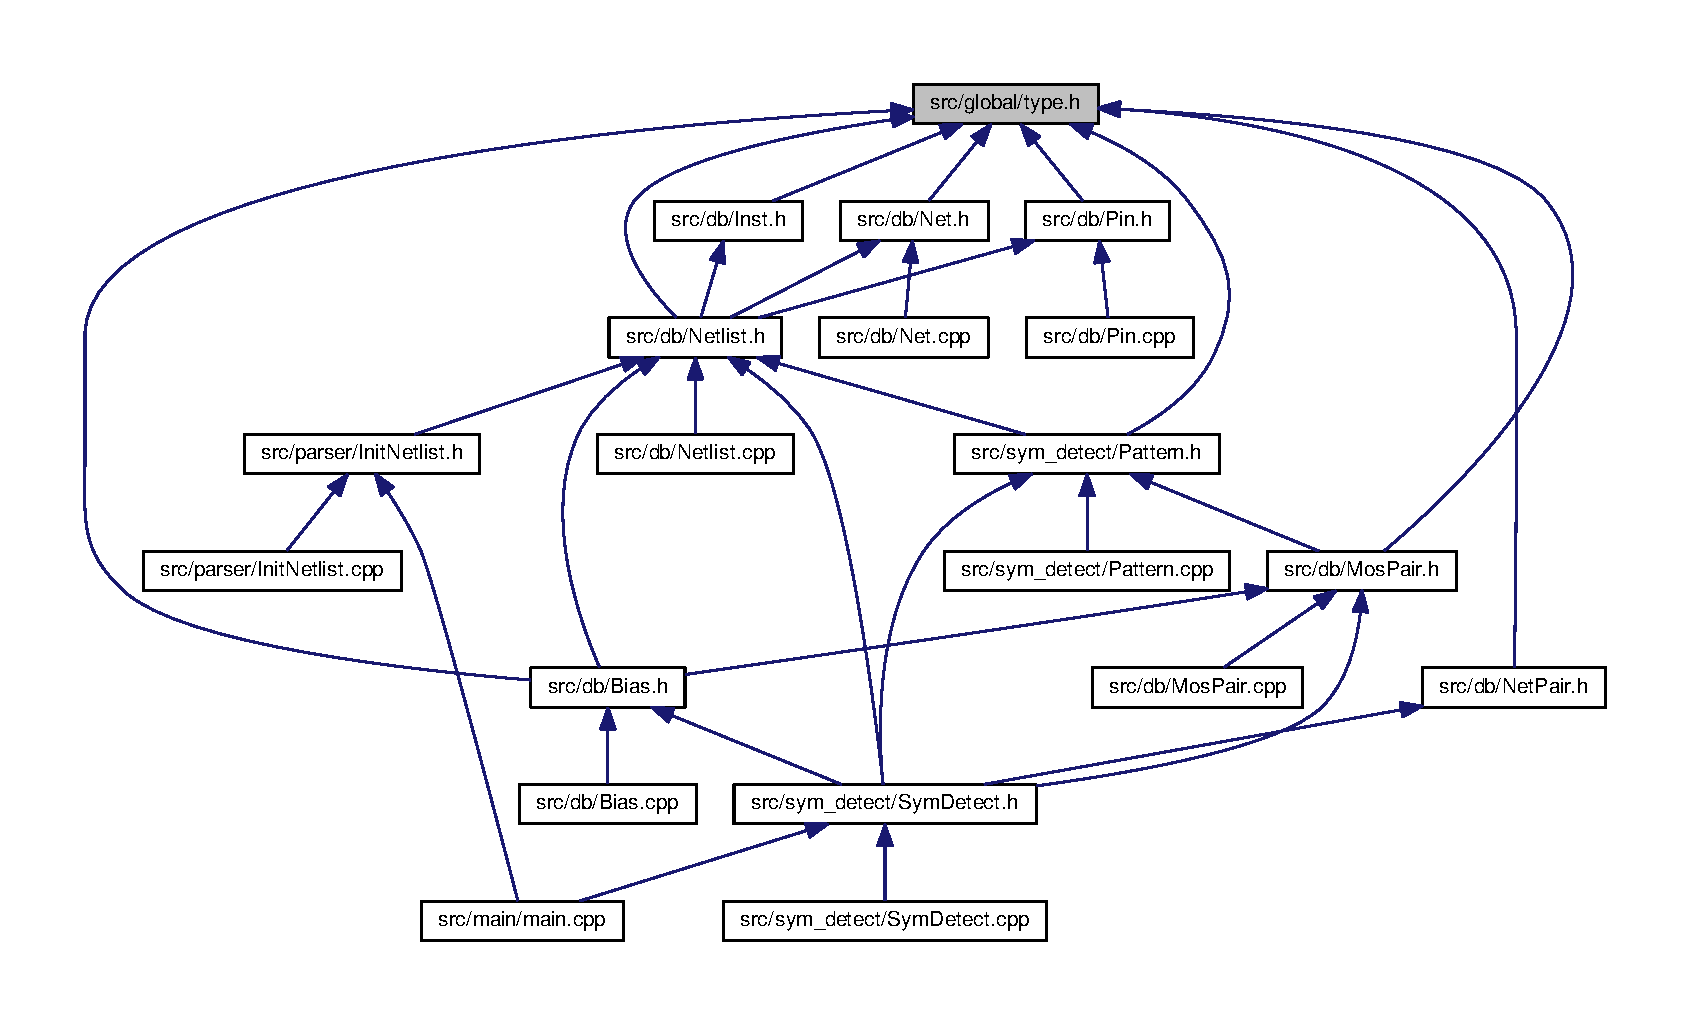
\includegraphics[width=350pt]{type_8h__dep__incl}
\end{center}
\end{figure}
\subsection*{Typedefs}
\begin{DoxyCompactItemize}
\item 
using \hyperlink{type_8h_a581e8093e28e7362f2b6937296190676}{Index\+Type} = std\+::uint32\+\_\+t
\item 
using \hyperlink{type_8h_a2db224c368d26648b9a810adaaab4123}{Int\+Type} = std\+::int32\+\_\+t
\item 
using \hyperlink{type_8h_a51898ad9e46b1265f3fab67f7d4b04a2}{Real\+Type} = double
\item 
using \hyperlink{type_8h_adb8cabc4ac5b90ae59717ab14b0c9d7f}{Byte} = std\+::uint8\+\_\+t
\end{DoxyCompactItemize}
\subsection*{Enumerations}
\begin{DoxyCompactItemize}
\item 
enum \hyperlink{type_8h_a53644c687d6bc203d9d3d3ee70075f61}{Inst\+Type} \+: Byte \{ \newline
\hyperlink{type_8h_a53644c687d6bc203d9d3d3ee70075f61af8af55aaebfbde59fb3954b42cedcf60}{Inst\+Type\+::\+R\+ES}, 
\hyperlink{type_8h_a53644c687d6bc203d9d3d3ee70075f61a24e337dfeaa2e154ab5ac12e8eca5609}{Inst\+Type\+::\+P\+M\+OS}, 
\hyperlink{type_8h_a53644c687d6bc203d9d3d3ee70075f61a032a04390cdce604754d59728e3cccfb}{Inst\+Type\+::\+N\+M\+OS}, 
\hyperlink{type_8h_a53644c687d6bc203d9d3d3ee70075f61adb5ce5cb1b12edacae4584e881e1451f}{Inst\+Type\+::\+C\+AP}, 
\newline
\hyperlink{type_8h_a53644c687d6bc203d9d3d3ee70075f61a03570470bad94692ce93e32700d2e1cb}{Inst\+Type\+::\+O\+T\+H\+ER}
 \}\begin{DoxyCompactList}\small\item\em Type of \hyperlink{classInst}{Inst}. \end{DoxyCompactList}
\item 
enum \hyperlink{type_8h_a24f31c8c9240242bd5fa9a415806eabf}{Net\+Type} \+: Byte \{ \hyperlink{type_8h_a24f31c8c9240242bd5fa9a415806eabfac9c9c146c630ca5ef9197c73c032f4a6}{Net\+Type\+::\+P\+O\+W\+ER}, 
\hyperlink{type_8h_a24f31c8c9240242bd5fa9a415806eabfadedcb56e75fe1488e20865e0ea36d0b9}{Net\+Type\+::\+G\+R\+O\+U\+ND}, 
\hyperlink{type_8h_a24f31c8c9240242bd5fa9a415806eabfac023ee28e6cb71d64feec71f0cbac067}{Net\+Type\+::\+S\+I\+G\+N\+AL}
 \}\begin{DoxyCompactList}\small\item\em Type of \hyperlink{classNet}{Net}. \end{DoxyCompactList}
\item 
enum \hyperlink{type_8h_afaab50027002ecbb6c8ac27e727d1bb4}{Pin\+Type} \+: Byte \{ \newline
\hyperlink{type_8h_afaab50027002ecbb6c8ac27e727d1bb4ae60b4854b44ccfb2d92aa6f035171bb4}{Pin\+Type\+::\+S\+O\+U\+R\+CE}, 
\hyperlink{type_8h_afaab50027002ecbb6c8ac27e727d1bb4ad22e8f7ce637479aeffe9dab9ee7337d}{Pin\+Type\+::\+D\+R\+A\+IN}, 
\hyperlink{type_8h_afaab50027002ecbb6c8ac27e727d1bb4a1818cedf1c2bed8c63664cc8313b443c}{Pin\+Type\+::\+G\+A\+TE}, 
\hyperlink{type_8h_afaab50027002ecbb6c8ac27e727d1bb4a6d5b457ed4205e7f1144ef21b944e552}{Pin\+Type\+::\+B\+U\+LK}, 
\newline
\hyperlink{type_8h_afaab50027002ecbb6c8ac27e727d1bb4ac9f869114804f0a61ce9b03def9d71f5}{Pin\+Type\+::\+T\+H\+IS}, 
\hyperlink{type_8h_afaab50027002ecbb6c8ac27e727d1bb4a13d613e84b1e7d08d869695a750caf23}{Pin\+Type\+::\+T\+H\+AT}, 
\hyperlink{type_8h_afaab50027002ecbb6c8ac27e727d1bb4a03570470bad94692ce93e32700d2e1cb}{Pin\+Type\+::\+O\+T\+H\+ER}
 \}\begin{DoxyCompactList}\small\item\em Type of \hyperlink{classPin}{Pin}. \end{DoxyCompactList}
\item 
enum \hyperlink{type_8h_a34a6a66323cfecf83dfe00bc8fd96333}{Mos\+Type} \+: Byte \{ \hyperlink{type_8h_a34a6a66323cfecf83dfe00bc8fd96333aa2e1ec2dd3d8195d238c5494f0ac5578}{Mos\+Type\+::\+D\+I\+FF}, 
\hyperlink{type_8h_a34a6a66323cfecf83dfe00bc8fd96333a27a3be7c1707f2fc3e9df9054eed8b4e}{Mos\+Type\+::\+D\+I\+O\+DE}, 
\hyperlink{type_8h_a34a6a66323cfecf83dfe00bc8fd96333adb5ce5cb1b12edacae4584e881e1451f}{Mos\+Type\+::\+C\+AP}, 
\hyperlink{type_8h_a34a6a66323cfecf83dfe00bc8fd96333abd2103035a8021942390a78a431ba0c4}{Mos\+Type\+::\+D\+U\+M\+MY}
 \}\begin{DoxyCompactList}\small\item\em Connection type of Mosfet. \end{DoxyCompactList}
\item 
enum \hyperlink{type_8h_af19eddb079bfea723256710b029c38e8}{Mos\+Pattern} \+: Byte \{ \newline
\hyperlink{type_8h_af19eddb079bfea723256710b029c38e8ad45b64a7d6b85dde1b52dd5a18863933}{Mos\+Pattern\+::\+D\+I\+F\+F\+\_\+\+S\+O\+U\+R\+CE}, 
\hyperlink{type_8h_af19eddb079bfea723256710b029c38e8a1b7b3de4c92d42d8311e04be030655af}{Mos\+Pattern\+::\+D\+I\+F\+F\+\_\+\+C\+A\+S\+C\+O\+DE}, 
\hyperlink{type_8h_af19eddb079bfea723256710b029c38e8aac50017227efb09ec529757764e5187c}{Mos\+Pattern\+::\+C\+A\+S\+C\+O\+DE}, 
\hyperlink{type_8h_af19eddb079bfea723256710b029c38e8a615d2885ef7576cedd9aafbb2578f028}{Mos\+Pattern\+::\+L\+O\+AD}, 
\newline
\hyperlink{type_8h_af19eddb079bfea723256710b029c38e8adb952aa3809767bf108688a754ebbf2c}{Mos\+Pattern\+::\+C\+R\+O\+S\+S\+\_\+\+C\+A\+S\+C\+O\+DE}, 
\hyperlink{type_8h_af19eddb079bfea723256710b029c38e8a19ddbfeab78ac1a4bbe1a186828c5d8d}{Mos\+Pattern\+::\+C\+R\+O\+S\+S\+\_\+\+L\+O\+AD}, 
\hyperlink{type_8h_af19eddb079bfea723256710b029c38e8ade1c70a20d797811b2fd32facf64bbd4}{Mos\+Pattern\+::\+P\+A\+S\+S\+I\+VE}, 
\hyperlink{type_8h_af19eddb079bfea723256710b029c38e8abe5470eb0ca5e3845ed08a1b358a5fb9}{Mos\+Pattern\+::\+S\+E\+LF}, 
\newline
\hyperlink{type_8h_af19eddb079bfea723256710b029c38e8ab8d9b53a9ce0cd78a9c3813faa792bbf}{Mos\+Pattern\+::\+B\+I\+AS}, 
\hyperlink{type_8h_af19eddb079bfea723256710b029c38e8accc0377a8afbf50e7094f5c23a8af223}{Mos\+Pattern\+::\+I\+N\+V\+A\+L\+ID}
 \}\begin{DoxyCompactList}\small\item\em \hyperlink{classPattern}{Pattern} for pair of Mosfet. \end{DoxyCompactList}
\end{DoxyCompactItemize}
\subsection*{Variables}
\begin{DoxyCompactItemize}
\item 
constexpr \hyperlink{type_8h_a581e8093e28e7362f2b6937296190676}{Index\+Type} \hyperlink{type_8h_a11591ec4ef05af2b0f48545966a61500}{I\+N\+D\+E\+X\+\_\+\+T\+Y\+P\+E\+\_\+\+M\+AX} = 1000000000
\item 
constexpr \hyperlink{type_8h_a2db224c368d26648b9a810adaaab4123}{Int\+Type} \hyperlink{type_8h_a7153b937cb94620c55b52fd559d1073e}{I\+N\+T\+\_\+\+T\+Y\+P\+E\+\_\+\+M\+AX} = 1000000000
\item 
constexpr \hyperlink{type_8h_a2db224c368d26648b9a810adaaab4123}{Int\+Type} \hyperlink{type_8h_ab6731eb941a9db9a459729271b27199e}{I\+N\+T\+\_\+\+T\+Y\+P\+E\+\_\+\+M\+IN} = -\/1000000000
\item 
constexpr \hyperlink{type_8h_a51898ad9e46b1265f3fab67f7d4b04a2}{Real\+Type} \hyperlink{type_8h_a68e54c8b6af80e1289b13eccd51be234}{R\+E\+A\+L\+\_\+\+T\+Y\+P\+E\+\_\+\+M\+AX} = 1e100
\item 
constexpr \hyperlink{type_8h_a51898ad9e46b1265f3fab67f7d4b04a2}{Real\+Type} \hyperlink{type_8h_aa2991a1c8de5bff9c42fc634a5839df1}{R\+E\+A\+L\+\_\+\+T\+Y\+P\+E\+\_\+\+M\+IN} = -\/1e100
\item 
constexpr \hyperlink{type_8h_a51898ad9e46b1265f3fab67f7d4b04a2}{Real\+Type} \hyperlink{type_8h_abe9e9223b325a4a377d3d6a2c752d199}{R\+E\+A\+L\+\_\+\+T\+Y\+P\+E\+\_\+\+T\+OL} = 1e-\/6
\end{DoxyCompactItemize}


\subsection{Detailed Description}
Type header file. 

\begin{DoxyAuthor}{Author}
Mingjie Liu 
\end{DoxyAuthor}
\begin{DoxyDate}{Date}
11/24/2018 
\end{DoxyDate}


\subsection{Typedef Documentation}
\mbox{\Hypertarget{type_8h_adb8cabc4ac5b90ae59717ab14b0c9d7f}\label{type_8h_adb8cabc4ac5b90ae59717ab14b0c9d7f}} 
\index{type.\+h@{type.\+h}!Byte@{Byte}}
\index{Byte@{Byte}!type.\+h@{type.\+h}}
\subsubsection{\texorpdfstring{Byte}{Byte}}
{\footnotesize\ttfamily using \hyperlink{type_8h_adb8cabc4ac5b90ae59717ab14b0c9d7f}{Byte} =  std\+::uint8\+\_\+t}

\mbox{\Hypertarget{type_8h_a581e8093e28e7362f2b6937296190676}\label{type_8h_a581e8093e28e7362f2b6937296190676}} 
\index{type.\+h@{type.\+h}!Index\+Type@{Index\+Type}}
\index{Index\+Type@{Index\+Type}!type.\+h@{type.\+h}}
\subsubsection{\texorpdfstring{Index\+Type}{IndexType}}
{\footnotesize\ttfamily using \hyperlink{type_8h_a581e8093e28e7362f2b6937296190676}{Index\+Type} =  std\+::uint32\+\_\+t}

\mbox{\Hypertarget{type_8h_a2db224c368d26648b9a810adaaab4123}\label{type_8h_a2db224c368d26648b9a810adaaab4123}} 
\index{type.\+h@{type.\+h}!Int\+Type@{Int\+Type}}
\index{Int\+Type@{Int\+Type}!type.\+h@{type.\+h}}
\subsubsection{\texorpdfstring{Int\+Type}{IntType}}
{\footnotesize\ttfamily using \hyperlink{type_8h_a2db224c368d26648b9a810adaaab4123}{Int\+Type} =  std\+::int32\+\_\+t}

\mbox{\Hypertarget{type_8h_a51898ad9e46b1265f3fab67f7d4b04a2}\label{type_8h_a51898ad9e46b1265f3fab67f7d4b04a2}} 
\index{type.\+h@{type.\+h}!Real\+Type@{Real\+Type}}
\index{Real\+Type@{Real\+Type}!type.\+h@{type.\+h}}
\subsubsection{\texorpdfstring{Real\+Type}{RealType}}
{\footnotesize\ttfamily using \hyperlink{type_8h_a51898ad9e46b1265f3fab67f7d4b04a2}{Real\+Type} =  double}



\subsection{Enumeration Type Documentation}
\mbox{\Hypertarget{type_8h_a53644c687d6bc203d9d3d3ee70075f61}\label{type_8h_a53644c687d6bc203d9d3d3ee70075f61}} 
\index{type.\+h@{type.\+h}!Inst\+Type@{Inst\+Type}}
\index{Inst\+Type@{Inst\+Type}!type.\+h@{type.\+h}}
\subsubsection{\texorpdfstring{Inst\+Type}{InstType}}
{\footnotesize\ttfamily enum \hyperlink{type_8h_a53644c687d6bc203d9d3d3ee70075f61}{Inst\+Type} \+: \hyperlink{type_8h_adb8cabc4ac5b90ae59717ab14b0c9d7f}{Byte}\hspace{0.3cm}{\ttfamily [strong]}}



Type of \hyperlink{classInst}{Inst}. 

\begin{DoxyEnumFields}{Enumerator}
\raisebox{\heightof{T}}[0pt][0pt]{\index{R\+ES@{R\+ES}!type.\+h@{type.\+h}}\index{type.\+h@{type.\+h}!R\+ES@{R\+ES}}}\mbox{\Hypertarget{type_8h_a53644c687d6bc203d9d3d3ee70075f61af8af55aaebfbde59fb3954b42cedcf60}\label{type_8h_a53644c687d6bc203d9d3d3ee70075f61af8af55aaebfbde59fb3954b42cedcf60}} 
R\+ES&Resistor \\
\hline

\raisebox{\heightof{T}}[0pt][0pt]{\index{P\+M\+OS@{P\+M\+OS}!type.\+h@{type.\+h}}\index{type.\+h@{type.\+h}!P\+M\+OS@{P\+M\+OS}}}\mbox{\Hypertarget{type_8h_a53644c687d6bc203d9d3d3ee70075f61a24e337dfeaa2e154ab5ac12e8eca5609}\label{type_8h_a53644c687d6bc203d9d3d3ee70075f61a24e337dfeaa2e154ab5ac12e8eca5609}} 
P\+M\+OS&P\+Mos \\
\hline

\raisebox{\heightof{T}}[0pt][0pt]{\index{N\+M\+OS@{N\+M\+OS}!type.\+h@{type.\+h}}\index{type.\+h@{type.\+h}!N\+M\+OS@{N\+M\+OS}}}\mbox{\Hypertarget{type_8h_a53644c687d6bc203d9d3d3ee70075f61a032a04390cdce604754d59728e3cccfb}\label{type_8h_a53644c687d6bc203d9d3d3ee70075f61a032a04390cdce604754d59728e3cccfb}} 
N\+M\+OS&N\+Mos \\
\hline

\raisebox{\heightof{T}}[0pt][0pt]{\index{C\+AP@{C\+AP}!type.\+h@{type.\+h}}\index{type.\+h@{type.\+h}!C\+AP@{C\+AP}}}\mbox{\Hypertarget{type_8h_a53644c687d6bc203d9d3d3ee70075f61adb5ce5cb1b12edacae4584e881e1451f}\label{type_8h_a53644c687d6bc203d9d3d3ee70075f61adb5ce5cb1b12edacae4584e881e1451f}} 
C\+AP&Capacitor \\
\hline

\raisebox{\heightof{T}}[0pt][0pt]{\index{O\+T\+H\+ER@{O\+T\+H\+ER}!type.\+h@{type.\+h}}\index{type.\+h@{type.\+h}!O\+T\+H\+ER@{O\+T\+H\+ER}}}\mbox{\Hypertarget{type_8h_a53644c687d6bc203d9d3d3ee70075f61a03570470bad94692ce93e32700d2e1cb}\label{type_8h_a53644c687d6bc203d9d3d3ee70075f61a03570470bad94692ce93e32700d2e1cb}} 
O\+T\+H\+ER&Other \\
\hline

\end{DoxyEnumFields}
\mbox{\Hypertarget{type_8h_af19eddb079bfea723256710b029c38e8}\label{type_8h_af19eddb079bfea723256710b029c38e8}} 
\index{type.\+h@{type.\+h}!Mos\+Pattern@{Mos\+Pattern}}
\index{Mos\+Pattern@{Mos\+Pattern}!type.\+h@{type.\+h}}
\subsubsection{\texorpdfstring{Mos\+Pattern}{MosPattern}}
{\footnotesize\ttfamily enum \hyperlink{type_8h_af19eddb079bfea723256710b029c38e8}{Mos\+Pattern} \+: \hyperlink{type_8h_adb8cabc4ac5b90ae59717ab14b0c9d7f}{Byte}\hspace{0.3cm}{\ttfamily [strong]}}



\hyperlink{classPattern}{Pattern} for pair of Mosfet. 

The patterns have been augmented to also handle self symmetry pairs and passive devices. The name retains as legacy.

\begin{DoxySeeAlso}{See also}
\hyperlink{classPattern_a1214e024706aff22e44bb4f4266d8e97}{Pattern\+::pattern()} 
\end{DoxySeeAlso}
\begin{DoxyEnumFields}{Enumerator}
\raisebox{\heightof{T}}[0pt][0pt]{\index{D\+I\+F\+F\+\_\+\+S\+O\+U\+R\+CE@{D\+I\+F\+F\+\_\+\+S\+O\+U\+R\+CE}!type.\+h@{type.\+h}}\index{type.\+h@{type.\+h}!D\+I\+F\+F\+\_\+\+S\+O\+U\+R\+CE@{D\+I\+F\+F\+\_\+\+S\+O\+U\+R\+CE}}}\mbox{\Hypertarget{type_8h_af19eddb079bfea723256710b029c38e8ad45b64a7d6b85dde1b52dd5a18863933}\label{type_8h_af19eddb079bfea723256710b029c38e8ad45b64a7d6b85dde1b52dd5a18863933}} 
D\+I\+F\+F\+\_\+\+S\+O\+U\+R\+CE&Source connected diff pair. \\
\hline

\raisebox{\heightof{T}}[0pt][0pt]{\index{D\+I\+F\+F\+\_\+\+C\+A\+S\+C\+O\+DE@{D\+I\+F\+F\+\_\+\+C\+A\+S\+C\+O\+DE}!type.\+h@{type.\+h}}\index{type.\+h@{type.\+h}!D\+I\+F\+F\+\_\+\+C\+A\+S\+C\+O\+DE@{D\+I\+F\+F\+\_\+\+C\+A\+S\+C\+O\+DE}}}\mbox{\Hypertarget{type_8h_af19eddb079bfea723256710b029c38e8a1b7b3de4c92d42d8311e04be030655af}\label{type_8h_af19eddb079bfea723256710b029c38e8a1b7b3de4c92d42d8311e04be030655af}} 
D\+I\+F\+F\+\_\+\+C\+A\+S\+C\+O\+DE&Cascode diff pair. \\
\hline

\raisebox{\heightof{T}}[0pt][0pt]{\index{C\+A\+S\+C\+O\+DE@{C\+A\+S\+C\+O\+DE}!type.\+h@{type.\+h}}\index{type.\+h@{type.\+h}!C\+A\+S\+C\+O\+DE@{C\+A\+S\+C\+O\+DE}}}\mbox{\Hypertarget{type_8h_af19eddb079bfea723256710b029c38e8aac50017227efb09ec529757764e5187c}\label{type_8h_af19eddb079bfea723256710b029c38e8aac50017227efb09ec529757764e5187c}} 
C\+A\+S\+C\+O\+DE&Gate connected cascode pair. \\
\hline

\raisebox{\heightof{T}}[0pt][0pt]{\index{L\+O\+AD@{L\+O\+AD}!type.\+h@{type.\+h}}\index{type.\+h@{type.\+h}!L\+O\+AD@{L\+O\+AD}}}\mbox{\Hypertarget{type_8h_af19eddb079bfea723256710b029c38e8a615d2885ef7576cedd9aafbb2578f028}\label{type_8h_af19eddb079bfea723256710b029c38e8a615d2885ef7576cedd9aafbb2578f028}} 
L\+O\+AD&Cascode pair with source connected to Power/\+Ground. \\
\hline

\raisebox{\heightof{T}}[0pt][0pt]{\index{C\+R\+O\+S\+S\+\_\+\+C\+A\+S\+C\+O\+DE@{C\+R\+O\+S\+S\+\_\+\+C\+A\+S\+C\+O\+DE}!type.\+h@{type.\+h}}\index{type.\+h@{type.\+h}!C\+R\+O\+S\+S\+\_\+\+C\+A\+S\+C\+O\+DE@{C\+R\+O\+S\+S\+\_\+\+C\+A\+S\+C\+O\+DE}}}\mbox{\Hypertarget{type_8h_af19eddb079bfea723256710b029c38e8adb952aa3809767bf108688a754ebbf2c}\label{type_8h_af19eddb079bfea723256710b029c38e8adb952aa3809767bf108688a754ebbf2c}} 
C\+R\+O\+S\+S\+\_\+\+C\+A\+S\+C\+O\+DE&Cross coupled cascode pair. \\
\hline

\raisebox{\heightof{T}}[0pt][0pt]{\index{C\+R\+O\+S\+S\+\_\+\+L\+O\+AD@{C\+R\+O\+S\+S\+\_\+\+L\+O\+AD}!type.\+h@{type.\+h}}\index{type.\+h@{type.\+h}!C\+R\+O\+S\+S\+\_\+\+L\+O\+AD@{C\+R\+O\+S\+S\+\_\+\+L\+O\+AD}}}\mbox{\Hypertarget{type_8h_af19eddb079bfea723256710b029c38e8a19ddbfeab78ac1a4bbe1a186828c5d8d}\label{type_8h_af19eddb079bfea723256710b029c38e8a19ddbfeab78ac1a4bbe1a186828c5d8d}} 
C\+R\+O\+S\+S\+\_\+\+L\+O\+AD&Cross coupled load. \\
\hline

\raisebox{\heightof{T}}[0pt][0pt]{\index{P\+A\+S\+S\+I\+VE@{P\+A\+S\+S\+I\+VE}!type.\+h@{type.\+h}}\index{type.\+h@{type.\+h}!P\+A\+S\+S\+I\+VE@{P\+A\+S\+S\+I\+VE}}}\mbox{\Hypertarget{type_8h_af19eddb079bfea723256710b029c38e8ade1c70a20d797811b2fd32facf64bbd4}\label{type_8h_af19eddb079bfea723256710b029c38e8ade1c70a20d797811b2fd32facf64bbd4}} 
P\+A\+S\+S\+I\+VE&Matched passive device. \\
\hline

\raisebox{\heightof{T}}[0pt][0pt]{\index{S\+E\+LF@{S\+E\+LF}!type.\+h@{type.\+h}}\index{type.\+h@{type.\+h}!S\+E\+LF@{S\+E\+LF}}}\mbox{\Hypertarget{type_8h_af19eddb079bfea723256710b029c38e8abe5470eb0ca5e3845ed08a1b358a5fb9}\label{type_8h_af19eddb079bfea723256710b029c38e8abe5470eb0ca5e3845ed08a1b358a5fb9}} 
S\+E\+LF&Self symmetry \hyperlink{classInst}{Inst}. \\
\hline

\raisebox{\heightof{T}}[0pt][0pt]{\index{B\+I\+AS@{B\+I\+AS}!type.\+h@{type.\+h}}\index{type.\+h@{type.\+h}!B\+I\+AS@{B\+I\+AS}}}\mbox{\Hypertarget{type_8h_af19eddb079bfea723256710b029c38e8ab8d9b53a9ce0cd78a9c3813faa792bbf}\label{type_8h_af19eddb079bfea723256710b029c38e8ab8d9b53a9ce0cd78a9c3813faa792bbf}} 
B\+I\+AS&\hyperlink{classBias}{Bias} symmetry pair. \\
\hline

\raisebox{\heightof{T}}[0pt][0pt]{\index{I\+N\+V\+A\+L\+ID@{I\+N\+V\+A\+L\+ID}!type.\+h@{type.\+h}}\index{type.\+h@{type.\+h}!I\+N\+V\+A\+L\+ID@{I\+N\+V\+A\+L\+ID}}}\mbox{\Hypertarget{type_8h_af19eddb079bfea723256710b029c38e8accc0377a8afbf50e7094f5c23a8af223}\label{type_8h_af19eddb079bfea723256710b029c38e8accc0377a8afbf50e7094f5c23a8af223}} 
I\+N\+V\+A\+L\+ID&No pattern detected. \\
\hline

\end{DoxyEnumFields}
\mbox{\Hypertarget{type_8h_a34a6a66323cfecf83dfe00bc8fd96333}\label{type_8h_a34a6a66323cfecf83dfe00bc8fd96333}} 
\index{type.\+h@{type.\+h}!Mos\+Type@{Mos\+Type}}
\index{Mos\+Type@{Mos\+Type}!type.\+h@{type.\+h}}
\subsubsection{\texorpdfstring{Mos\+Type}{MosType}}
{\footnotesize\ttfamily enum \hyperlink{type_8h_a34a6a66323cfecf83dfe00bc8fd96333}{Mos\+Type} \+: \hyperlink{type_8h_adb8cabc4ac5b90ae59717ab14b0c9d7f}{Byte}\hspace{0.3cm}{\ttfamily [strong]}}



Connection type of Mosfet. 

\begin{DoxySeeAlso}{See also}
\hyperlink{classNetlist_a3dba84b8588a528e42b066083744958f}{Netlist\+::mos\+Type()}. 
\end{DoxySeeAlso}
\begin{DoxyEnumFields}{Enumerator}
\raisebox{\heightof{T}}[0pt][0pt]{\index{D\+I\+FF@{D\+I\+FF}!type.\+h@{type.\+h}}\index{type.\+h@{type.\+h}!D\+I\+FF@{D\+I\+FF}}}\mbox{\Hypertarget{type_8h_a34a6a66323cfecf83dfe00bc8fd96333aa2e1ec2dd3d8195d238c5494f0ac5578}\label{type_8h_a34a6a66323cfecf83dfe00bc8fd96333aa2e1ec2dd3d8195d238c5494f0ac5578}} 
D\+I\+FF&D/\+G/S diff \\
\hline

\raisebox{\heightof{T}}[0pt][0pt]{\index{D\+I\+O\+DE@{D\+I\+O\+DE}!type.\+h@{type.\+h}}\index{type.\+h@{type.\+h}!D\+I\+O\+DE@{D\+I\+O\+DE}}}\mbox{\Hypertarget{type_8h_a34a6a66323cfecf83dfe00bc8fd96333a27a3be7c1707f2fc3e9df9054eed8b4e}\label{type_8h_a34a6a66323cfecf83dfe00bc8fd96333a27a3be7c1707f2fc3e9df9054eed8b4e}} 
D\+I\+O\+DE&G/D connected \\
\hline

\raisebox{\heightof{T}}[0pt][0pt]{\index{C\+AP@{C\+AP}!type.\+h@{type.\+h}}\index{type.\+h@{type.\+h}!C\+AP@{C\+AP}}}\mbox{\Hypertarget{type_8h_a34a6a66323cfecf83dfe00bc8fd96333adb5ce5cb1b12edacae4584e881e1451f}\label{type_8h_a34a6a66323cfecf83dfe00bc8fd96333adb5ce5cb1b12edacae4584e881e1451f}} 
C\+AP&G/S connected \\
\hline

\raisebox{\heightof{T}}[0pt][0pt]{\index{D\+U\+M\+MY@{D\+U\+M\+MY}!type.\+h@{type.\+h}}\index{type.\+h@{type.\+h}!D\+U\+M\+MY@{D\+U\+M\+MY}}}\mbox{\Hypertarget{type_8h_a34a6a66323cfecf83dfe00bc8fd96333abd2103035a8021942390a78a431ba0c4}\label{type_8h_a34a6a66323cfecf83dfe00bc8fd96333abd2103035a8021942390a78a431ba0c4}} 
D\+U\+M\+MY&D/S connected \\
\hline

\end{DoxyEnumFields}
\mbox{\Hypertarget{type_8h_a24f31c8c9240242bd5fa9a415806eabf}\label{type_8h_a24f31c8c9240242bd5fa9a415806eabf}} 
\index{type.\+h@{type.\+h}!Net\+Type@{Net\+Type}}
\index{Net\+Type@{Net\+Type}!type.\+h@{type.\+h}}
\subsubsection{\texorpdfstring{Net\+Type}{NetType}}
{\footnotesize\ttfamily enum \hyperlink{type_8h_a24f31c8c9240242bd5fa9a415806eabf}{Net\+Type} \+: \hyperlink{type_8h_adb8cabc4ac5b90ae59717ab14b0c9d7f}{Byte}\hspace{0.3cm}{\ttfamily [strong]}}



Type of \hyperlink{classNet}{Net}. 

\begin{DoxyEnumFields}{Enumerator}
\raisebox{\heightof{T}}[0pt][0pt]{\index{P\+O\+W\+ER@{P\+O\+W\+ER}!type.\+h@{type.\+h}}\index{type.\+h@{type.\+h}!P\+O\+W\+ER@{P\+O\+W\+ER}}}\mbox{\Hypertarget{type_8h_a24f31c8c9240242bd5fa9a415806eabfac9c9c146c630ca5ef9197c73c032f4a6}\label{type_8h_a24f31c8c9240242bd5fa9a415806eabfac9c9c146c630ca5ef9197c73c032f4a6}} 
P\+O\+W\+ER&Power \\
\hline

\raisebox{\heightof{T}}[0pt][0pt]{\index{G\+R\+O\+U\+ND@{G\+R\+O\+U\+ND}!type.\+h@{type.\+h}}\index{type.\+h@{type.\+h}!G\+R\+O\+U\+ND@{G\+R\+O\+U\+ND}}}\mbox{\Hypertarget{type_8h_a24f31c8c9240242bd5fa9a415806eabfadedcb56e75fe1488e20865e0ea36d0b9}\label{type_8h_a24f31c8c9240242bd5fa9a415806eabfadedcb56e75fe1488e20865e0ea36d0b9}} 
G\+R\+O\+U\+ND&Ground \\
\hline

\raisebox{\heightof{T}}[0pt][0pt]{\index{S\+I\+G\+N\+AL@{S\+I\+G\+N\+AL}!type.\+h@{type.\+h}}\index{type.\+h@{type.\+h}!S\+I\+G\+N\+AL@{S\+I\+G\+N\+AL}}}\mbox{\Hypertarget{type_8h_a24f31c8c9240242bd5fa9a415806eabfac023ee28e6cb71d64feec71f0cbac067}\label{type_8h_a24f31c8c9240242bd5fa9a415806eabfac023ee28e6cb71d64feec71f0cbac067}} 
S\+I\+G\+N\+AL&Signal \\
\hline

\end{DoxyEnumFields}
\mbox{\Hypertarget{type_8h_afaab50027002ecbb6c8ac27e727d1bb4}\label{type_8h_afaab50027002ecbb6c8ac27e727d1bb4}} 
\index{type.\+h@{type.\+h}!Pin\+Type@{Pin\+Type}}
\index{Pin\+Type@{Pin\+Type}!type.\+h@{type.\+h}}
\subsubsection{\texorpdfstring{Pin\+Type}{PinType}}
{\footnotesize\ttfamily enum \hyperlink{type_8h_afaab50027002ecbb6c8ac27e727d1bb4}{Pin\+Type} \+: \hyperlink{type_8h_adb8cabc4ac5b90ae59717ab14b0c9d7f}{Byte}\hspace{0.3cm}{\ttfamily [strong]}}



Type of \hyperlink{classPin}{Pin}. 

\begin{DoxyEnumFields}{Enumerator}
\raisebox{\heightof{T}}[0pt][0pt]{\index{S\+O\+U\+R\+CE@{S\+O\+U\+R\+CE}!type.\+h@{type.\+h}}\index{type.\+h@{type.\+h}!S\+O\+U\+R\+CE@{S\+O\+U\+R\+CE}}}\mbox{\Hypertarget{type_8h_afaab50027002ecbb6c8ac27e727d1bb4ae60b4854b44ccfb2d92aa6f035171bb4}\label{type_8h_afaab50027002ecbb6c8ac27e727d1bb4ae60b4854b44ccfb2d92aa6f035171bb4}} 
S\+O\+U\+R\+CE&\hyperlink{classInst}{Inst} is Mosfet \\
\hline

\raisebox{\heightof{T}}[0pt][0pt]{\index{D\+R\+A\+IN@{D\+R\+A\+IN}!type.\+h@{type.\+h}}\index{type.\+h@{type.\+h}!D\+R\+A\+IN@{D\+R\+A\+IN}}}\mbox{\Hypertarget{type_8h_afaab50027002ecbb6c8ac27e727d1bb4ad22e8f7ce637479aeffe9dab9ee7337d}\label{type_8h_afaab50027002ecbb6c8ac27e727d1bb4ad22e8f7ce637479aeffe9dab9ee7337d}} 
D\+R\+A\+IN&\hyperlink{classInst}{Inst} is Mosfet \\
\hline

\raisebox{\heightof{T}}[0pt][0pt]{\index{G\+A\+TE@{G\+A\+TE}!type.\+h@{type.\+h}}\index{type.\+h@{type.\+h}!G\+A\+TE@{G\+A\+TE}}}\mbox{\Hypertarget{type_8h_afaab50027002ecbb6c8ac27e727d1bb4a1818cedf1c2bed8c63664cc8313b443c}\label{type_8h_afaab50027002ecbb6c8ac27e727d1bb4a1818cedf1c2bed8c63664cc8313b443c}} 
G\+A\+TE&\hyperlink{classInst}{Inst} is Mosfet \\
\hline

\raisebox{\heightof{T}}[0pt][0pt]{\index{B\+U\+LK@{B\+U\+LK}!type.\+h@{type.\+h}}\index{type.\+h@{type.\+h}!B\+U\+LK@{B\+U\+LK}}}\mbox{\Hypertarget{type_8h_afaab50027002ecbb6c8ac27e727d1bb4a6d5b457ed4205e7f1144ef21b944e552}\label{type_8h_afaab50027002ecbb6c8ac27e727d1bb4a6d5b457ed4205e7f1144ef21b944e552}} 
B\+U\+LK&\hyperlink{classInst}{Inst} is Mosfet \\
\hline

\raisebox{\heightof{T}}[0pt][0pt]{\index{T\+H\+IS@{T\+H\+IS}!type.\+h@{type.\+h}}\index{type.\+h@{type.\+h}!T\+H\+IS@{T\+H\+IS}}}\mbox{\Hypertarget{type_8h_afaab50027002ecbb6c8ac27e727d1bb4ac9f869114804f0a61ce9b03def9d71f5}\label{type_8h_afaab50027002ecbb6c8ac27e727d1bb4ac9f869114804f0a61ce9b03def9d71f5}} 
T\+H\+IS&\hyperlink{classInst}{Inst} is Passive \\
\hline

\raisebox{\heightof{T}}[0pt][0pt]{\index{T\+H\+AT@{T\+H\+AT}!type.\+h@{type.\+h}}\index{type.\+h@{type.\+h}!T\+H\+AT@{T\+H\+AT}}}\mbox{\Hypertarget{type_8h_afaab50027002ecbb6c8ac27e727d1bb4a13d613e84b1e7d08d869695a750caf23}\label{type_8h_afaab50027002ecbb6c8ac27e727d1bb4a13d613e84b1e7d08d869695a750caf23}} 
T\+H\+AT&\hyperlink{classInst}{Inst} is Passive \\
\hline

\raisebox{\heightof{T}}[0pt][0pt]{\index{O\+T\+H\+ER@{O\+T\+H\+ER}!type.\+h@{type.\+h}}\index{type.\+h@{type.\+h}!O\+T\+H\+ER@{O\+T\+H\+ER}}}\mbox{\Hypertarget{type_8h_afaab50027002ecbb6c8ac27e727d1bb4a03570470bad94692ce93e32700d2e1cb}\label{type_8h_afaab50027002ecbb6c8ac27e727d1bb4a03570470bad94692ce93e32700d2e1cb}} 
O\+T\+H\+ER&Other \\
\hline

\end{DoxyEnumFields}


\subsection{Variable Documentation}
\mbox{\Hypertarget{type_8h_a11591ec4ef05af2b0f48545966a61500}\label{type_8h_a11591ec4ef05af2b0f48545966a61500}} 
\index{type.\+h@{type.\+h}!I\+N\+D\+E\+X\+\_\+\+T\+Y\+P\+E\+\_\+\+M\+AX@{I\+N\+D\+E\+X\+\_\+\+T\+Y\+P\+E\+\_\+\+M\+AX}}
\index{I\+N\+D\+E\+X\+\_\+\+T\+Y\+P\+E\+\_\+\+M\+AX@{I\+N\+D\+E\+X\+\_\+\+T\+Y\+P\+E\+\_\+\+M\+AX}!type.\+h@{type.\+h}}
\subsubsection{\texorpdfstring{I\+N\+D\+E\+X\+\_\+\+T\+Y\+P\+E\+\_\+\+M\+AX}{INDEX\_TYPE\_MAX}}
{\footnotesize\ttfamily constexpr \hyperlink{type_8h_a581e8093e28e7362f2b6937296190676}{Index\+Type} I\+N\+D\+E\+X\+\_\+\+T\+Y\+P\+E\+\_\+\+M\+AX = 1000000000}

\mbox{\Hypertarget{type_8h_a7153b937cb94620c55b52fd559d1073e}\label{type_8h_a7153b937cb94620c55b52fd559d1073e}} 
\index{type.\+h@{type.\+h}!I\+N\+T\+\_\+\+T\+Y\+P\+E\+\_\+\+M\+AX@{I\+N\+T\+\_\+\+T\+Y\+P\+E\+\_\+\+M\+AX}}
\index{I\+N\+T\+\_\+\+T\+Y\+P\+E\+\_\+\+M\+AX@{I\+N\+T\+\_\+\+T\+Y\+P\+E\+\_\+\+M\+AX}!type.\+h@{type.\+h}}
\subsubsection{\texorpdfstring{I\+N\+T\+\_\+\+T\+Y\+P\+E\+\_\+\+M\+AX}{INT\_TYPE\_MAX}}
{\footnotesize\ttfamily constexpr \hyperlink{type_8h_a2db224c368d26648b9a810adaaab4123}{Int\+Type} I\+N\+T\+\_\+\+T\+Y\+P\+E\+\_\+\+M\+AX = 1000000000}

\mbox{\Hypertarget{type_8h_ab6731eb941a9db9a459729271b27199e}\label{type_8h_ab6731eb941a9db9a459729271b27199e}} 
\index{type.\+h@{type.\+h}!I\+N\+T\+\_\+\+T\+Y\+P\+E\+\_\+\+M\+IN@{I\+N\+T\+\_\+\+T\+Y\+P\+E\+\_\+\+M\+IN}}
\index{I\+N\+T\+\_\+\+T\+Y\+P\+E\+\_\+\+M\+IN@{I\+N\+T\+\_\+\+T\+Y\+P\+E\+\_\+\+M\+IN}!type.\+h@{type.\+h}}
\subsubsection{\texorpdfstring{I\+N\+T\+\_\+\+T\+Y\+P\+E\+\_\+\+M\+IN}{INT\_TYPE\_MIN}}
{\footnotesize\ttfamily constexpr \hyperlink{type_8h_a2db224c368d26648b9a810adaaab4123}{Int\+Type} I\+N\+T\+\_\+\+T\+Y\+P\+E\+\_\+\+M\+IN = -\/1000000000}

\mbox{\Hypertarget{type_8h_a68e54c8b6af80e1289b13eccd51be234}\label{type_8h_a68e54c8b6af80e1289b13eccd51be234}} 
\index{type.\+h@{type.\+h}!R\+E\+A\+L\+\_\+\+T\+Y\+P\+E\+\_\+\+M\+AX@{R\+E\+A\+L\+\_\+\+T\+Y\+P\+E\+\_\+\+M\+AX}}
\index{R\+E\+A\+L\+\_\+\+T\+Y\+P\+E\+\_\+\+M\+AX@{R\+E\+A\+L\+\_\+\+T\+Y\+P\+E\+\_\+\+M\+AX}!type.\+h@{type.\+h}}
\subsubsection{\texorpdfstring{R\+E\+A\+L\+\_\+\+T\+Y\+P\+E\+\_\+\+M\+AX}{REAL\_TYPE\_MAX}}
{\footnotesize\ttfamily constexpr \hyperlink{type_8h_a51898ad9e46b1265f3fab67f7d4b04a2}{Real\+Type} R\+E\+A\+L\+\_\+\+T\+Y\+P\+E\+\_\+\+M\+AX = 1e100}

\mbox{\Hypertarget{type_8h_aa2991a1c8de5bff9c42fc634a5839df1}\label{type_8h_aa2991a1c8de5bff9c42fc634a5839df1}} 
\index{type.\+h@{type.\+h}!R\+E\+A\+L\+\_\+\+T\+Y\+P\+E\+\_\+\+M\+IN@{R\+E\+A\+L\+\_\+\+T\+Y\+P\+E\+\_\+\+M\+IN}}
\index{R\+E\+A\+L\+\_\+\+T\+Y\+P\+E\+\_\+\+M\+IN@{R\+E\+A\+L\+\_\+\+T\+Y\+P\+E\+\_\+\+M\+IN}!type.\+h@{type.\+h}}
\subsubsection{\texorpdfstring{R\+E\+A\+L\+\_\+\+T\+Y\+P\+E\+\_\+\+M\+IN}{REAL\_TYPE\_MIN}}
{\footnotesize\ttfamily constexpr \hyperlink{type_8h_a51898ad9e46b1265f3fab67f7d4b04a2}{Real\+Type} R\+E\+A\+L\+\_\+\+T\+Y\+P\+E\+\_\+\+M\+IN = -\/1e100}

\mbox{\Hypertarget{type_8h_abe9e9223b325a4a377d3d6a2c752d199}\label{type_8h_abe9e9223b325a4a377d3d6a2c752d199}} 
\index{type.\+h@{type.\+h}!R\+E\+A\+L\+\_\+\+T\+Y\+P\+E\+\_\+\+T\+OL@{R\+E\+A\+L\+\_\+\+T\+Y\+P\+E\+\_\+\+T\+OL}}
\index{R\+E\+A\+L\+\_\+\+T\+Y\+P\+E\+\_\+\+T\+OL@{R\+E\+A\+L\+\_\+\+T\+Y\+P\+E\+\_\+\+T\+OL}!type.\+h@{type.\+h}}
\subsubsection{\texorpdfstring{R\+E\+A\+L\+\_\+\+T\+Y\+P\+E\+\_\+\+T\+OL}{REAL\_TYPE\_TOL}}
{\footnotesize\ttfamily constexpr \hyperlink{type_8h_a51898ad9e46b1265f3fab67f7d4b04a2}{Real\+Type} R\+E\+A\+L\+\_\+\+T\+Y\+P\+E\+\_\+\+T\+OL = 1e-\/6}


\hypertarget{main_8cpp}{}\section{src/main/main.cpp File Reference}
\label{main_8cpp}\index{src/main/main.\+cpp@{src/main/main.\+cpp}}


\hyperlink{main_8cpp}{main.\+cpp}  


{\ttfamily \#include $<$string$>$}\newline
{\ttfamily \#include $<$iostream$>$}\newline
{\ttfamily \#include $<$vector$>$}\newline
{\ttfamily \#include \char`\"{}parser/\+Init\+Netlist.\+h\char`\"{}}\newline
{\ttfamily \#include \char`\"{}sym\+\_\+detect/\+Sym\+Detect.\+h\char`\"{}}\newline
Include dependency graph for main.\+cpp\+:
\nopagebreak
\begin{figure}[H]
\begin{center}
\leavevmode
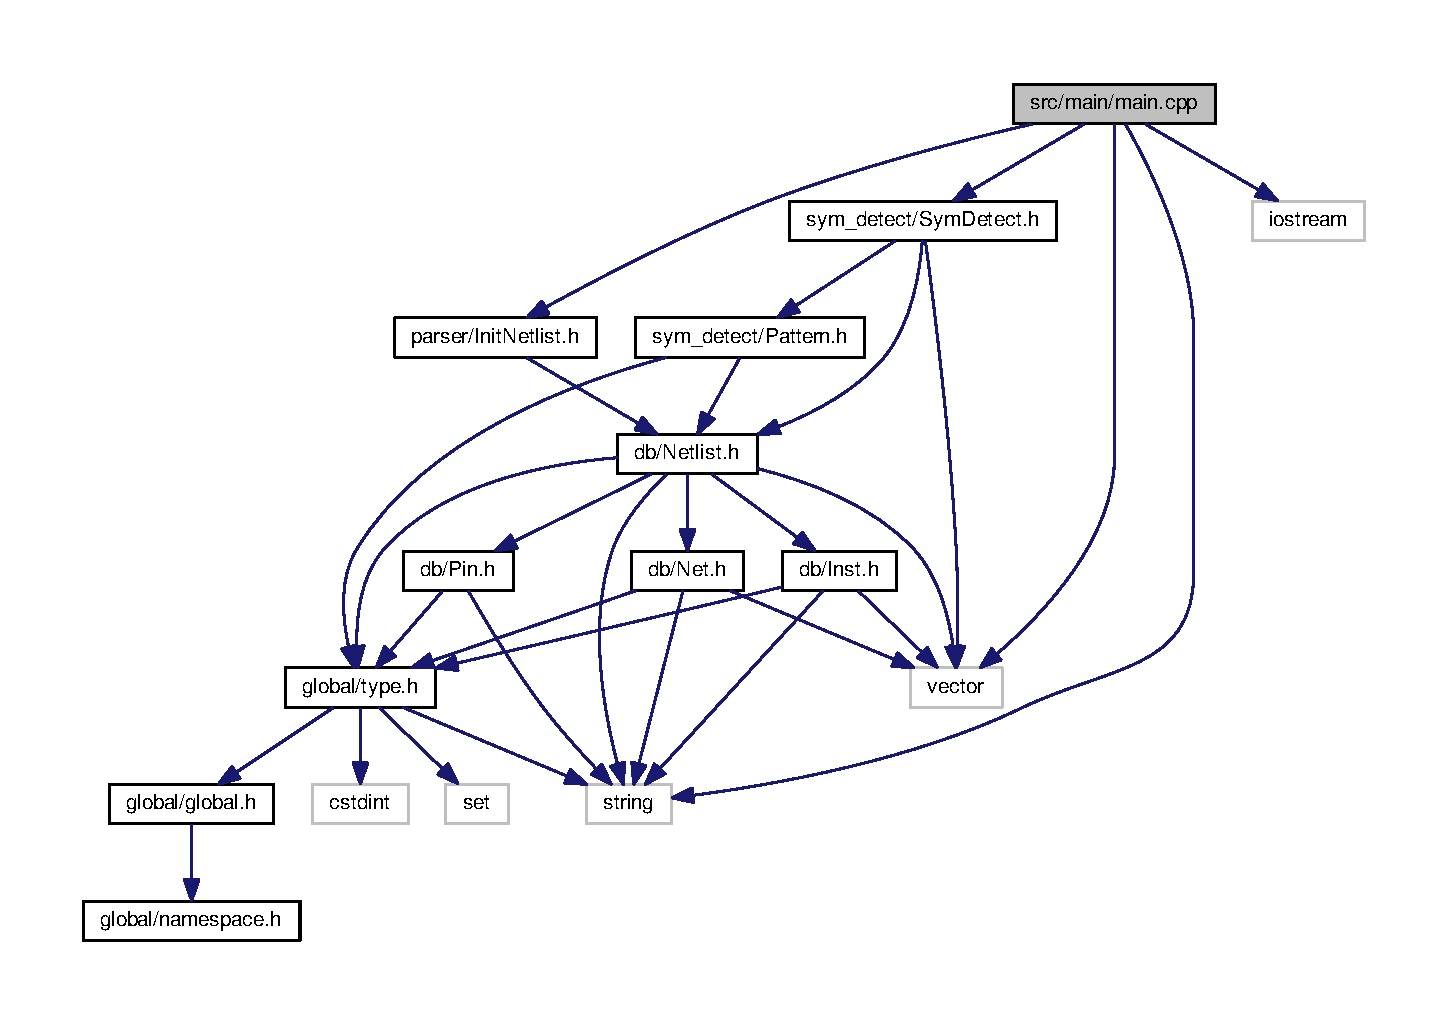
\includegraphics[width=350pt]{main_8cpp__incl}
\end{center}
\end{figure}
\subsection*{Macros}
\begin{DoxyCompactItemize}
\item 
\#define \hyperlink{main_8cpp_af69acb595306f7146bb66498c43ef407}{\+\_\+\+\_\+\+S\+F\+A\+\_\+\+T\+E\+S\+T\+\_\+\+\_\+}
\end{DoxyCompactItemize}
\subsection*{Functions}
\begin{DoxyCompactItemize}
\item 
int \hyperlink{main_8cpp_a0ddf1224851353fc92bfbff6f499fa97}{main} (int argc, char $\ast$argv\mbox{[}$\,$\mbox{]})
\end{DoxyCompactItemize}


\subsection{Detailed Description}
\hyperlink{main_8cpp}{main.\+cpp} 

\begin{DoxyAuthor}{Author}
Mingjie L\+Iu 
\end{DoxyAuthor}
\begin{DoxyDate}{Date}
11/25/2018
\end{DoxyDate}
Takes 1 argument input. Parse the file into \hyperlink{classNetlist}{Netlist}. Detect hierarchy symmetry groups and print to command line. Input file should be of certain format. See \hyperlink{InitNetlist_8h}{parser/\+Init\+Netlist.\+h} for details. 

\subsection{Macro Definition Documentation}
\mbox{\Hypertarget{main_8cpp_af69acb595306f7146bb66498c43ef407}\label{main_8cpp_af69acb595306f7146bb66498c43ef407}} 
\index{main.\+cpp@{main.\+cpp}!\+\_\+\+\_\+\+S\+F\+A\+\_\+\+T\+E\+S\+T\+\_\+\+\_\+@{\+\_\+\+\_\+\+S\+F\+A\+\_\+\+T\+E\+S\+T\+\_\+\+\_\+}}
\index{\+\_\+\+\_\+\+S\+F\+A\+\_\+\+T\+E\+S\+T\+\_\+\+\_\+@{\+\_\+\+\_\+\+S\+F\+A\+\_\+\+T\+E\+S\+T\+\_\+\+\_\+}!main.\+cpp@{main.\+cpp}}
\subsubsection{\texorpdfstring{\+\_\+\+\_\+\+S\+F\+A\+\_\+\+T\+E\+S\+T\+\_\+\+\_\+}{\_\_SFA\_TEST\_\_}}
{\footnotesize\ttfamily \#define \+\_\+\+\_\+\+S\+F\+A\+\_\+\+T\+E\+S\+T\+\_\+\+\_\+}



\subsection{Function Documentation}
\mbox{\Hypertarget{main_8cpp_a0ddf1224851353fc92bfbff6f499fa97}\label{main_8cpp_a0ddf1224851353fc92bfbff6f499fa97}} 
\index{main.\+cpp@{main.\+cpp}!main@{main}}
\index{main@{main}!main.\+cpp@{main.\+cpp}}
\subsubsection{\texorpdfstring{main()}{main()}}
{\footnotesize\ttfamily int main (\begin{DoxyParamCaption}\item[{int}]{argc,  }\item[{char $\ast$}]{argv\mbox{[}$\,$\mbox{]} }\end{DoxyParamCaption})}


\hypertarget{InitNetlist_8cpp}{}\section{src/parser/\+Init\+Netlist.cpp File Reference}
\label{InitNetlist_8cpp}\index{src/parser/\+Init\+Netlist.\+cpp@{src/parser/\+Init\+Netlist.\+cpp}}


Parser implementation.  


{\ttfamily \#include $<$cstdio$>$}\newline
{\ttfamily \#include $<$fstream$>$}\newline
{\ttfamily \#include \char`\"{}Init\+Netlist.\+h\char`\"{}}\newline
Include dependency graph for Init\+Netlist.\+cpp\+:
\nopagebreak
\begin{figure}[H]
\begin{center}
\leavevmode
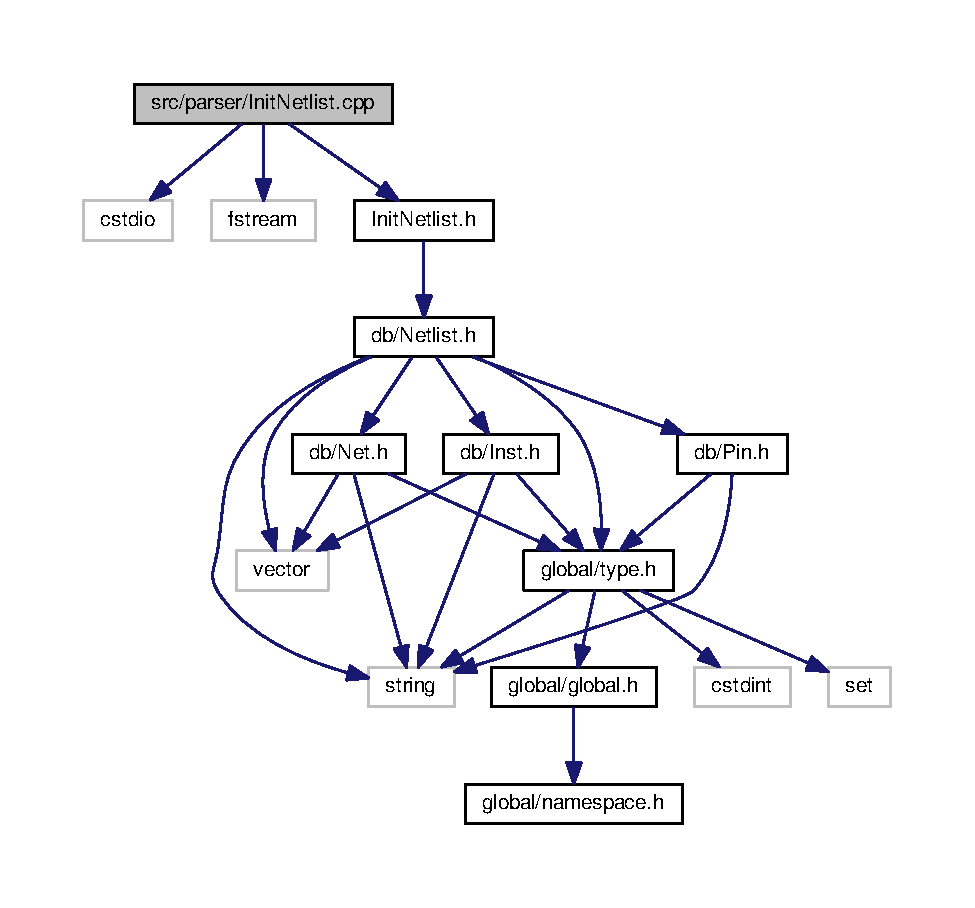
\includegraphics[width=350pt]{InitNetlist_8cpp__incl}
\end{center}
\end{figure}


\subsection{Detailed Description}
Parser implementation. 

\begin{DoxyAuthor}{Author}
Mingjie Liu 
\end{DoxyAuthor}
\begin{DoxyDate}{Date}
11/24/2018 
\end{DoxyDate}

\hypertarget{InitNetlist_8h}{}\section{src/parser/\+Init\+Netlist.h File Reference}
\label{InitNetlist_8h}\index{src/parser/\+Init\+Netlist.\+h@{src/parser/\+Init\+Netlist.\+h}}


Parser to initialize netlist.  


{\ttfamily \#include \char`\"{}db/\+Netlist.\+h\char`\"{}}\newline
Include dependency graph for Init\+Netlist.\+h\+:\nopagebreak
\begin{figure}[H]
\begin{center}
\leavevmode
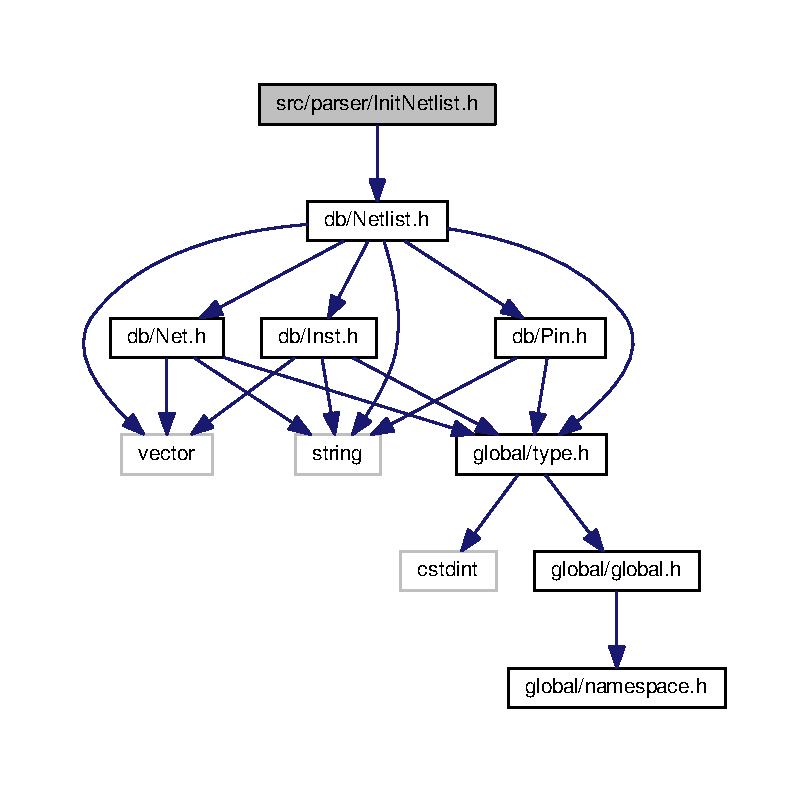
\includegraphics[width=350pt]{InitNetlist_8h__incl}
\end{center}
\end{figure}
This graph shows which files directly or indirectly include this file\+:\nopagebreak
\begin{figure}[H]
\begin{center}
\leavevmode
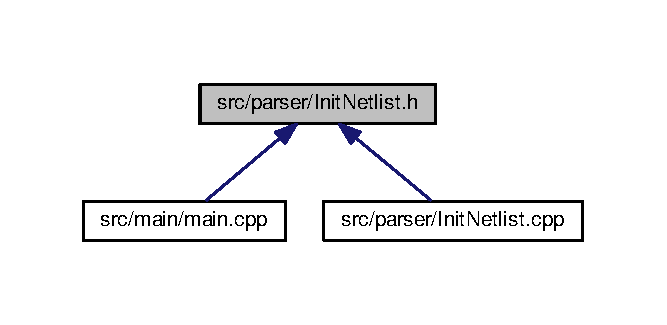
\includegraphics[width=320pt]{InitNetlist_8h__dep__incl}
\end{center}
\end{figure}
\subsection*{Classes}
\begin{DoxyCompactItemize}
\item 
class \hyperlink{classInitNetlist}{Init\+Netlist}
\begin{DoxyCompactList}\small\item\em \hyperlink{classInitNetlist}{Init\+Netlist} class. \end{DoxyCompactList}\end{DoxyCompactItemize}


\subsection{Detailed Description}
Parser to initialize netlist. 

\begin{DoxyAuthor}{Author}
Mingjie Liu 
\end{DoxyAuthor}
\begin{DoxyDate}{Date}
11/24/2018
\end{DoxyDate}
Input file should follow same format generated through scripts/create\+\_\+init\+\_\+obj.\+py. The python scripts take standardized hspice/spectre netlist files as inputs. Sample input files for c++ are under benchmarks. 
\hypertarget{Pattern_8cpp}{}\section{src/sym\+\_\+detect/\+Pattern.cpp File Reference}
\label{Pattern_8cpp}\index{src/sym\+\_\+detect/\+Pattern.\+cpp@{src/sym\+\_\+detect/\+Pattern.\+cpp}}


\hyperlink{classPattern}{Pattern} definitions.  


{\ttfamily \#include \char`\"{}sym\+\_\+detect/\+Pattern.\+h\char`\"{}}\newline
Include dependency graph for Pattern.\+cpp\+:\nopagebreak
\begin{figure}[H]
\begin{center}
\leavevmode
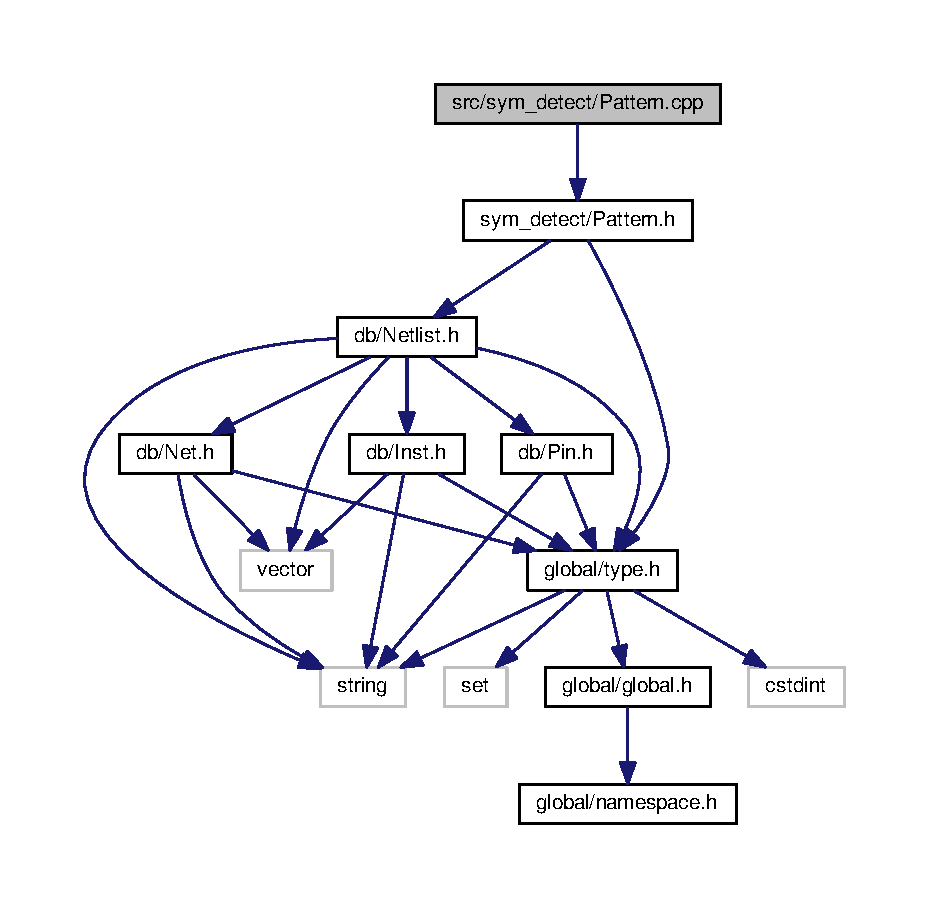
\includegraphics[width=350pt]{Pattern_8cpp__incl}
\end{center}
\end{figure}


\subsection{Detailed Description}
\hyperlink{classPattern}{Pattern} definitions. 

\begin{DoxyAuthor}{Author}
Mingjie Liu 
\end{DoxyAuthor}
\begin{DoxyDate}{Date}
11/24/2018 
\end{DoxyDate}

\hypertarget{Pattern_8h}{}\section{src/sym\+\_\+detect/\+Pattern.h File Reference}
\label{Pattern_8h}\index{src/sym\+\_\+detect/\+Pattern.\+h@{src/sym\+\_\+detect/\+Pattern.\+h}}


Mosfet pair patterns.  


{\ttfamily \#include \char`\"{}db/\+Netlist.\+h\char`\"{}}\newline
{\ttfamily \#include \char`\"{}global/type.\+h\char`\"{}}\newline
Include dependency graph for Pattern.\+h\+:\nopagebreak
\begin{figure}[H]
\begin{center}
\leavevmode
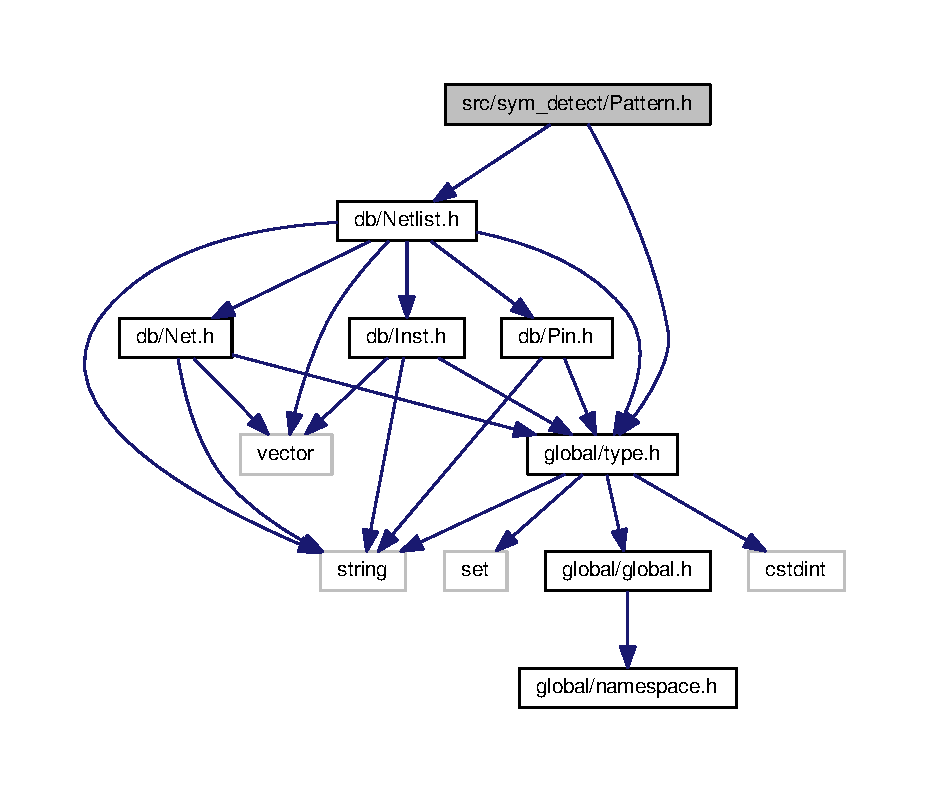
\includegraphics[width=350pt]{Pattern_8h__incl}
\end{center}
\end{figure}
This graph shows which files directly or indirectly include this file\+:
\nopagebreak
\begin{figure}[H]
\begin{center}
\leavevmode
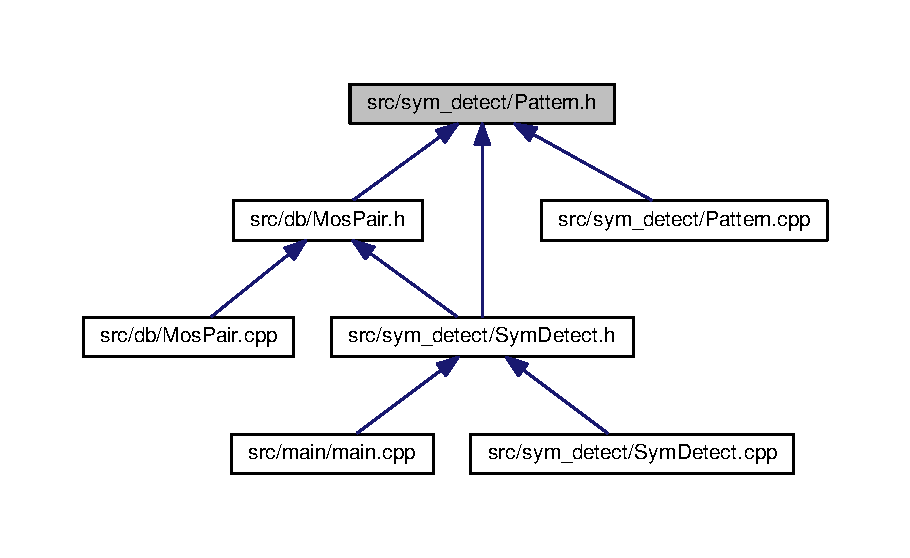
\includegraphics[width=350pt]{Pattern_8h__dep__incl}
\end{center}
\end{figure}
\subsection*{Classes}
\begin{DoxyCompactItemize}
\item 
class \hyperlink{classPattern}{Pattern}
\begin{DoxyCompactList}\small\item\em \hyperlink{classPattern}{Pattern} class. \end{DoxyCompactList}\end{DoxyCompactItemize}


\subsection{Detailed Description}
Mosfet pair patterns. 

This class has been augmented also to handle passive device matching and self symmetry mosfets. The name remains as legacy.

\begin{DoxyAuthor}{Author}
Mingjie Liu 
\end{DoxyAuthor}
\begin{DoxyDate}{Date}
11/24/2018 
\end{DoxyDate}

\hypertarget{SymDetect_8cpp}{}\section{src/sym\+\_\+detect/\+Sym\+Detect.cpp File Reference}
\label{SymDetect_8cpp}\index{src/sym\+\_\+detect/\+Sym\+Detect.\+cpp@{src/sym\+\_\+detect/\+Sym\+Detect.\+cpp}}


Detect symmetric patterns.  


{\ttfamily \#include \char`\"{}sym\+\_\+detect/\+Sym\+Detect.\+h\char`\"{}}\newline
Include dependency graph for Sym\+Detect.\+cpp\+:
\nopagebreak
\begin{figure}[H]
\begin{center}
\leavevmode
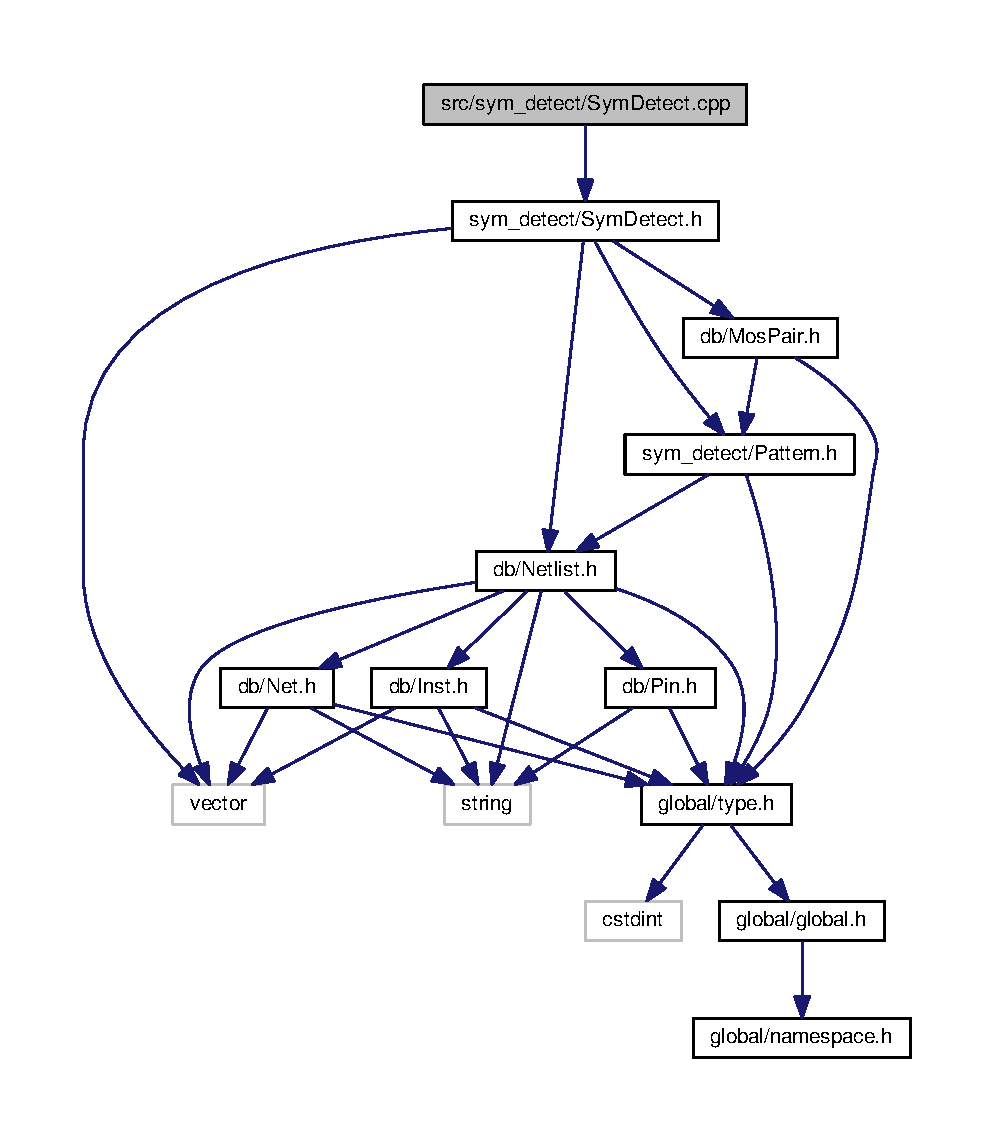
\includegraphics[width=350pt]{SymDetect_8cpp__incl}
\end{center}
\end{figure}


\subsection{Detailed Description}
Detect symmetric patterns. 

\begin{DoxyAuthor}{Author}
Mingjie Liu 
\end{DoxyAuthor}
\begin{DoxyDate}{Date}
11/24/2018 
\end{DoxyDate}

\hypertarget{SymDetect_8h}{}\section{src/sym\+\_\+detect/\+Sym\+Detect.h File Reference}
\label{SymDetect_8h}\index{src/sym\+\_\+detect/\+Sym\+Detect.\+h@{src/sym\+\_\+detect/\+Sym\+Detect.\+h}}


Detect symmetric patterns.  


{\ttfamily \#include \char`\"{}db/\+Netlist.\+h\char`\"{}}\newline
{\ttfamily \#include \char`\"{}db/\+Mos\+Pair.\+h\char`\"{}}\newline
{\ttfamily \#include \char`\"{}db/\+Net\+Pair.\+h\char`\"{}}\newline
{\ttfamily \#include \char`\"{}db/\+Bias.\+h\char`\"{}}\newline
{\ttfamily \#include \char`\"{}sym\+\_\+detect/\+Pattern.\+h\char`\"{}}\newline
{\ttfamily \#include $<$vector$>$}\newline
{\ttfamily \#include $<$string$>$}\newline
Include dependency graph for Sym\+Detect.\+h\+:
\nopagebreak
\begin{figure}[H]
\begin{center}
\leavevmode
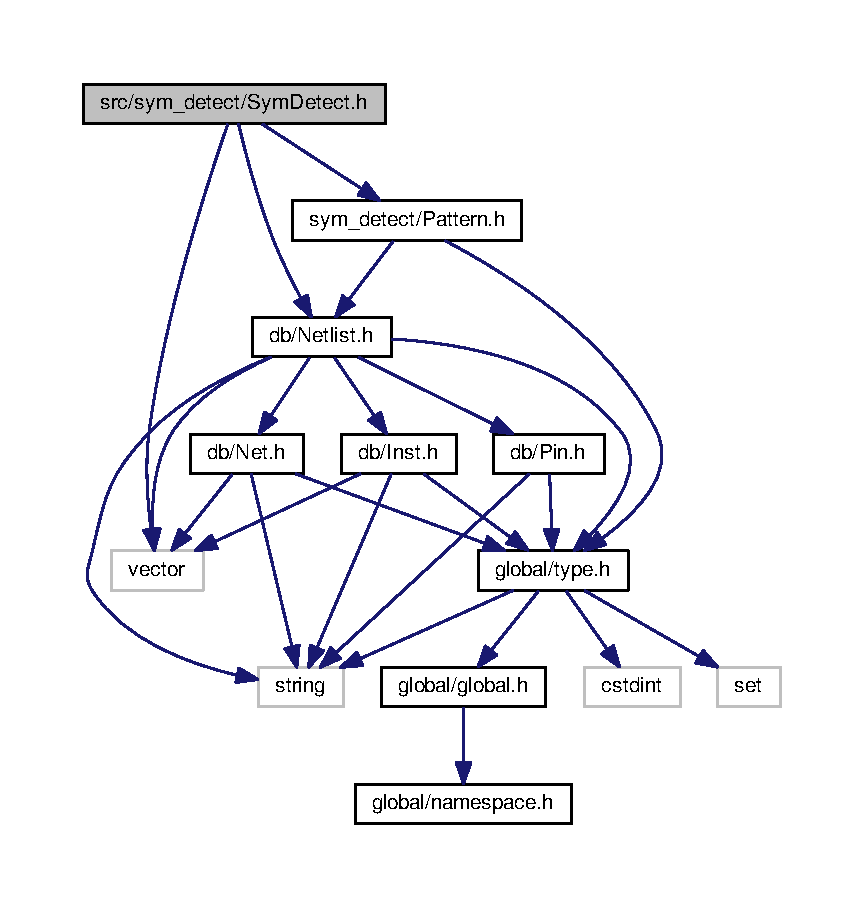
\includegraphics[width=350pt]{SymDetect_8h__incl}
\end{center}
\end{figure}
This graph shows which files directly or indirectly include this file\+:
\nopagebreak
\begin{figure}[H]
\begin{center}
\leavevmode
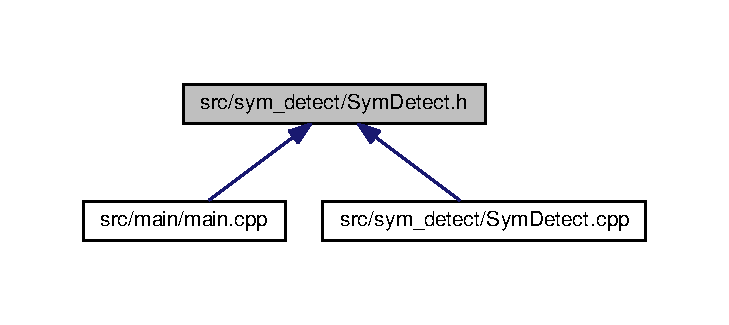
\includegraphics[width=350pt]{SymDetect_8h__dep__incl}
\end{center}
\end{figure}
\subsection*{Classes}
\begin{DoxyCompactItemize}
\item 
class \hyperlink{classSymDetect}{Sym\+Detect}
\begin{DoxyCompactList}\small\item\em \hyperlink{classSymDetect}{Sym\+Detect} class. \end{DoxyCompactList}\end{DoxyCompactItemize}


\subsection{Detailed Description}
Detect symmetric patterns. 

\begin{DoxyAuthor}{Author}
Mingjie Liu 
\end{DoxyAuthor}
\begin{DoxyDate}{Date}
11/24/2018 
\end{DoxyDate}

%--- End generated contents ---

% Index
\backmatter
\newpage
\phantomsection
\clearemptydoublepage
\addcontentsline{toc}{chapter}{Index}
\printindex

\end{document}
